\documentclass{book}

\usepackage{graphicx}
\usepackage{epstopdf}
\usepackage{url} % this package doesn't make proper clickable links, but
% \usepackage{hyperref} % this package breaks the build.
\usepackage{microtype}
\usepackage{amssymb}
\usepackage{framed} % for sidebars
\usepackage[includefoot]{geometry} % for margins
\usepackage{tocloft}  % to typeset table of contents
\usepackage{titlesec} % to format chapter title pages
\usepackage{fancyhdr} % to format headers/footers
\pagestyle{fancy}
\usepackage{sectsty}
\usepackage{wrapfig}

\usepackage[T1]{fontenc}
\usepackage{tgtermes}    % body font
\usepackage{inconsolata} % fixed width font
\usepackage{tgheros}     % sans-serif font

\author{Amy Brown \& Greg Wilson}

% define page size and margins etc
\geometry{paperwidth=18.91cm,paperheight=24.589cm,
          vmargin=1.9cm, % top and bottom margins
          inner=1.9cm, % inside margin
          outer=2.29cm, % outside margin
          bindingoffset=0.89cm % gutter
         } 

% define headers (empty) and footers
% fiddle with chaptermark so we can make it not all caps
\renewcommand{\chaptermark}[1]{\markboth{#1}{}}
\renewcommand{\sectionmark}[1]{\markright{#1}{}}

% next get rid of existing header and footer and header rule
\fancyhead{}
\fancyfoot{}
\renewcommand{\headrulewidth}{0pt}

% now make the footer the way we want it:
% page number on right side of footer for odd pages 
\rfoot[]{\small{\textsf{\chapterauthor \hspace{0.25cm} \thepage}}}
\fancyhfoffset[EL]{0cm} % this looks like it doesn't do anything, but
                        % it seems to remind it to line up headers with the
                        % rest of the text

% page number and chapter name on left side of footer for even pages 
\lfoot[\small{\textsf{\thepage \hspace{0.25cm} \leftmark}}]{}

% make plain pages have no headers or footers
\fancypagestyle{plain}{\fancyhf{}}

% set all section headers to be sans serif
\allsectionsfont{\normalfont\sffamily}

% format the table of contents
\renewcommand{\cftchapfont}{\sffamily}     % set TOC entries to sserif
\renewcommand{\cftchappagefont}{\sffamily} % set TOC page numbers to sserif

% make all verbatim (code blocks) text smaller, just because it was bugging me
\let\oldverbatim\verbatim
\renewcommand\verbatim{\small\oldverbatim}


% format title of TOC: make sure this matches chapter head format as set below
\renewcommand{\cfttoctitlefont}{\hfill\Huge\sffamily} 

\setcounter{tocdepth}{0} % sets what level of header is shown in the TOC
\setcounter{secnumdepth}{1} % sets what level of subsect. are numbered

% introduce penalty for widows and orphans (can increase to 10 000, although
% not recommended)
\widowpenalty=300
\clubpenalty=300

\title{The Architecture of Open Source Applications}
\date{}

\newcommand{\chapterauthor}{}

\newcommand{\chapterauthortoc}{}

\newenvironment{aosachapter}[3]
{ \renewcommand{\chapterauthor}{#3} \chapter{#1} \label{#2} 
   \addtocontents{toc}{\hspace{1cm}\textit{\textsf{by \chapterauthor}}\protect\par} } {  }

\newenvironment{aosachaptertoc}[4]
{ \renewcommand{\chapterauthor}{#3}
  \renewcommand{\chapterauthortoc}{#4}
  \chapter{#1} \label{#2} 
  \addtocontents{toc}{\hspace{1cm}\textit{\textsf{by \chapterauthortoc}}\protect\par} } {  }

\newenvironment{aosasect1}[1]{\section{#1}}{}
\newenvironment{aosasect2}[1]{\subsection{#1}}{}
\newenvironment{aosasect3}[1]{\subsubsection*{#1}}{}

\newenvironment{aosabox}[1]
{ \begin{figure}[h!]\vspace{-0.7cm}\centering \rule[-.7cm]{12.82cm}{0.75pt} \begin{minipage}[t]{12.82cm}\begin{framed}\centerline{{\textbf{#1}}} }
{ \end{framed}\end{minipage} \rule{12.82cm}{0.75pt} \end{figure} }

\newenvironment{aosadescription}
{\begin{description}\addtolength{\itemsep}{-0.6\baselineskip}}
{\end{description}}

\newenvironment{aosaenumerate}
{\begin{enumerate}\addtolength{\itemsep}{-0.6\baselineskip}}
{\end{enumerate}}

\newenvironment{aosaitemize}
{\begin{itemize}\addtolength{\itemsep}{-0.6\baselineskip}}
{\end{itemize}}

\newcommand{\aosaboxref}[1]{Box~\ref{#1}}
\newcommand{\aosachapref}[1]{Chapter~\ref{#1}}
\newcommand{\aosafigref}[1]{Figure~\ref{#1}}
\newcommand{\aosasecref}[1]{Section~\ref{#1}}
\newcommand{\aosatblref}[1]{Table~\ref{#1}}

\newcommand{\aosafigure}[4][375pt]{\begin{figure}[h!]\centering\includegraphics[width={#1}]{#2}\caption{#3}\label{#4}\end{figure}}
\newcommand{\aosafigureTop}[4][375pt]{\begin{figure}[t]\centering\includegraphics[width={#1}]{#2}\caption{#3}\label{#4}\end{figure}}

\newcommand{\aosagraphics}[2][375pt]{\includegraphics[width={#1}]{#2}}
\newcommand{\aosaquestion}[1]{\begin{textbf}{#1}\end{textbf}}
\newcommand{\code}[1]{\texttt{#1}}

% format chapter title pages
\titleformat{\chapter}
  [display] % shape/type of title
  {\sffamily} % formatting commands applied to both label and title
  {\vspace{-2cm} \hfill \Large Chapter \hspace{-0.2cm} \Huge \thechapter} 
  {2cm} % separation between number and chapter title
  {\Huge} % code preceding title. Last cmd can take arg, which is title
  [  % everything inside [] comes after the title
     % \hspace*{1cm} % indent author name 
     \Large % make text that follows large
     \thispagestyle{plain} % suppress page numbers
     \chapterauthor % insert chapter author name 
  ]% end of what comes after title

\raggedbottom

\begin{document}

% \frontmatter
% \newpage

% half title page
\thispagestyle{empty}
\hspace{-2cm}
% \includegraphics[width=400pt]{../images/frontmatter/title.eps}

\newpage

% Blank page here
\thispagestyle{empty}
\mbox{}    % need to have *something* in here or Latex "helpfully" removes page

\newpage
% title page

\thispagestyle{empty}
\hspace{-2cm}
% \includegraphics[width=400pt]{../images/frontmatter/title.eps}
\\
\vspace{0.5cm}
\hspace{2.8cm}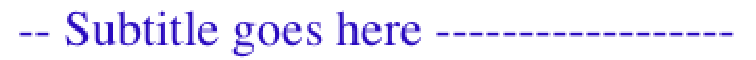
\includegraphics{../images/frontmatter/subtitle.pdf}
\\[13.5cm]
\vspace{0.5cm}
\hspace{6.5cm}
%\includegraphics{../images/frontmatter/eds.eps}

\newpage
% copyright page

\thispagestyle{empty}

\small
\noindent \textbf{The Architecture of Open Source Applications, Volume 2} \\
Edited by Amy Brown and Greg Wilson

\vspace{0.15cm}

\noindent
This work is licensed under the Creative Commons Attribution 3.0
Unported license (CC~BY~3.0).  You are free:

\begin{aosaitemize}
  \item to Share---to copy, distribute and transmit the work
  \item to Remix---to adapt the work
\end{aosaitemize}

\noindent
under the following conditions:

\begin{aosaitemize}
  \item Attribution---you must attribute the work in the manner
    specified by the author or licensor (but not in any way that
    suggests that they endorse you or your use of the work).
\end{aosaitemize}

\noindent
with the understanding that:

\begin{aosaitemize}

  \item Waiver---Any of the above conditions can be waived if you get
    permission from the copyright holder.

  \item Public Domain---Where the work or any of its elements is in
    the public domain under applicable law, that status is in no way
    affected by the license.

  \item Other Rights---In no way are any of the following rights
    affected by the license:
    \begin{aosaitemize}

      \item Your fair dealing or fair use rights, or other applicable
        copyright exceptions and limitations;

      \item The author's moral rights;

      \item Rights other persons may have either in the work itself or
        in how the work is used, such as publicity or privacy rights.

    \end{aosaitemize}

  \item Notice---For any reuse or distribution, you must make clear to
    others the license terms of this work. The best way to do this is
    with a link to \url{http://creativecommons.org/licenses/by/3.0/}.

\end{aosaitemize}

\noindent To view a copy of this license, visit
\url{http://creativecommons.org/licenses/by/3.0/} or send a letter to Creative
Commons, 444 Castro Street, Suite 900, Mountain View, California,
94041, USA.\\

\vspace{0.15cm}

\noindent
The full text of this book is available online at \url{http://www.aosabook.org/}.\\
All royalties from its sale will be donated to Amnesty International.\\

\vfill

\noindent Product and company names mentioned herein may be the trademarks of
their respective owners.\\

\vspace{0.15cm}

\noindent While every precaution has been taken in the preparation of this
book, the editors and authors assume no responsibility for errors or omissions,
or for damages resulting from the use of the information contained herein.\\

\vspace{0.15cm}

\noindent Attribution and license for cover photo goes here. FIXME

\vspace{1cm}

\noindent Revision Date: \today \\

\noindent ISBN: New ISBN goes here - FIXME
\normalsize

\newpage
% Dedication page

\thispagestyle{empty}

\vspace*{5cm}
\begin{center}
\hspace{0cm}Dedication goes here. FIXME
\end{center}

\newpage

% Blank page here
\thispagestyle{empty}
\mbox{}    % need to have *something* in here or Latex "helpfully" removes page



\tableofcontents

\begin{aosachapter}{Introduction}{s:intro}{Amy Brown and Greg Wilson}

Mention \cite{bib:aosa1}.

\section*{Contributors}

\emph{Andrey Alexeev (nginx)}: FIXME

\emph{Chris AtLee (Firefox Release Engineering)}: FIXME

\emph{Michael Bayer (SQLAlchemy)}: FIXME

\emph{Lukas Blakk (Firefox Release Engineering)}: FIXME

\emph{Amy Brown (editorial)}: Amy worked in the software industry for
ten years before decamping to create a freelance editing and book production
business. She has an underused degree in Math, two small children, a
husband and a cat. She can be found online at \url{http://www.arbrown.ca/}

\emph{Sheeri Cabral (Database Evolution)}: FIXME

\emph{Jon Cruz (Inkscape)}: FIXME

\emph{Selena Deckelmann (PostgreSQL)}: FIXME

\emph{Michael Droettboom (matplotlib)}: FIXME

\emph{Tiago Espinha (Apache Derby)}: FIXME

\emph{Elizabeth Flanagan (Yocto)}: FIXME

\emph{Jeff Hardy (Iron Languages)}: FIXME

\emph{Sumana Harihareswara (MediaWiki)}: FIXME

\emph{Elise Huard (Erlang VM)}: FIXME

\emph{Tim Hunt (Moodle)}: FIXME

\emph{John Hunter (matplotlib)}: FIXME

\emph{Luis Ibanez (ITK)}: Luis has worked for 11 years on the development of
the Insight Toolkit (ITK), an open source library for medical imaging analysis.
Luis is a strong supporter of open access and the revival of reproducibiliy
verification in scientific publishing. Luis has been teaching a course on Open
Source Software Practices at Rensselaer since 2007.

\emph{Mike Kamermans (Processing.js)}: FIXME

\emph{Luke Kanies (Puppet)}: FIXME

\emph{Nigel Kersten (Puppet)}: FIXME

\emph{Brad King (ITK)}: FIXME

\emph{Simon Marlow (The Glasgow Haskell Compiler)}: FIXME

\emph{Kate Matsudaira ()}: FIXME

\emph{Jessica McKellar (Twisted)}: FIXME

\emph{Sarah Mei (Diaspora)}: FIXME

\emph{John O'Duinn (Firefox Release Engineering)}: FIXME

\emph{Addy Osmani (jQuery)}: FIXME

\emph{Christoph Otto (Parrot)}: FIXME

\emph{Guillaume Paumier (MediaWiki)}: FIXME

\emph{Benjamin Peterson (PyPy)}: FIXME

\emph{Simon Peyton-Jones (The Glasgow Haskell Compiler)}: FIXME

\emph{Susan Potter (Git)}: Susan is a polyglot software developer with
over 14 years of professional experience coding, building, designing,
maintaining and supporting production distributed systems in risk management,
market data and some front office application development for investment
banking, hedge fund and proprietary trading clients. Susan current defines the
system and application architecture, design, coding and testing standards for
a Platform as a Service (PaaS) firm providing hosted front and middle office
applications, web services and APIs.

\emph{Allison Randal (Linux Distribution)}: FIXME

\emph{Eric Raymond (GPSD)}: FIXME

\emph{Jennifer Ruttan (OSCAR)}: FIXME

\emph{Eugene Sandulenko (scummvm)}: FIXME

\emph{Stan Shebs (gdb)}: FIXME

\emph{Michael Snoyman (Yesod)}: FIXME

\emph{Jeff Squyres (Open MPI)}: FIXME

\emph{Martin Sustrik (ZeroMQ)}: FIXME

\emph{Christopher Svec (FreeRTOS)}: FIXME

\emph{James Turnbull (Puppet)}: FIXME

\emph{Jesse Vincent (K-9 Mail)}: FIXME

\emph{Barry Warsaw (Mailman)}: FIXME

\emph{Greg Wilson (editorial)}: Greg has worked over the past 25 years
in high-performance scientific computing, data visualization, and
computer security, and is the author or editor of several computing
books (including the 2008 Jolt Award winner \emph{Beautiful Code}) and
two books for children.  Greg received a Ph.D.\ in Computer Science
from the University of Edinburgh in 1993.

\emph{Harry Wood (OpenStreetMap)}: FIXME

\emph{Armen Zambrano Gasparnian (Firefox Release Engineering)}: FIXME

\section*{Acknowledgments}

FIXME

\section*{Contributing}

Dozens of volunteers worked hard to create this book, but there is
still a lot to do.  You can help by reporting errors, by helping to
translate the content into other languages, or by describing the
architecture of other open source projects.  Please contact us at
\code{aosa@aosabook.org} if you would like to get involved.

\end{aosachapter}


\mainmatter
\include{dbevol}
\include{diaspora}
\begin{aosachapter}{Scalable Web Architecture and Distributed Systems}{s:distsys}{Kate Matsudaira}

Open source software has become a fundamental building block for some
of the biggest websites. And as those websites have grown,
best practices and guiding principles around their architectures have
emerged. This chapter seeks to cover some of the key issues to
consider when designing large websites, as well as some of the
building blocks used to achieve these goals.

This chapter is largely focused on web systems, although some of the
material is applicable to other distributed systems as well.

\begin{aosasect1}{Principles of Web Distributed Systems Design}

What exactly does it mean to build and operate a scalable web site or
application? At a primitive level it's just connecting users with remote
resources via the Internet---the part that makes it scalable is
that the resources, or access to those resources, are distributed
across multiple servers.

Like most things in life, taking the time to plan ahead when building a
web service can help in
the long run; 
understanding some of the considerations and tradeoffs behind big
websites can result in smarter decisions at the creation of
smaller web sites. Below are some of the key principles that influence
the design of large-scale web systems:

\begin{aosadescription}

\item{Availability:} The uptime of a website is absolutely critical to
  the reputation and functional of many companies. For some of the
  larger online retail sites, being unavailable for even minutes can
  result in thousands or millions of dollars in lost revenue, so
  designing their systems to be constantly available and resilient to
  failure is both a fundamental business and a technology
  requirement. High availability in distributed systems requires the
  careful consideration of redundancy for key components, rapid
  recovery in the event of partial system failures, and graceful
  degradation when problems occur.

\item{Performance:} Website performance has become an important
  consideration for most sites. The speed of a website affects
  usage and user satisfaction, as well as search engine rankings, a
  factor that directly correlates to revenue and retention. As a
  result, creating a system that is optimized for fast responses and
  low latency is key.

\item{Reliability:} A system needs to be reliable, such that a request
  for data will consistently return the same data. In the event the
  data changes or is updated, then that same request should return the
  new data. Users need to know that if something is written to the
  system, or stored, it will persist and can be relied on to be in
  place for future retrieval.

\item{Scalability:} When it comes to any large distributed system, 
  size is just one aspect of scale that needs to be considered. Just as
  important is the effort required to increase capacity to handle
  greater amounts of load, commonly referred to as the
  scalability of the system. Scalability can refer to many different
  parameters of the system: how much additional traffic can it
  handle, how easy is it to add more storage capacity, or even how
  many more transactions can be processed.

\item{Manageability:} Designing a system that
  is easy to operate is another important consideration.  The manageability of
  the system equates to the scalability of operations: maintenance and
  updates. Things to consider for manageability are the ease of diagnosing and
  understanding problems when they occur, ease of making updates or
  modifications, and how simple the system is to operate. (I.e., does it
  routinely operate without failure or exceptions?)

\item{Cost:} Cost is an important factor. This obviously
  can include hardware and software costs, but it is also important to
  consider other facets needed to deploy and maintain the
  system. The amount of developer time the system takes to
  build, the amount of operational effort required to run the system,
  and even the amount of training required should all be
  considered. Cost is the total cost of ownership.

\end{aosadescription}

Each of these principles provides the basis for decisions 
in designing a distributed web architecture. However, they also can
be at odds with one another, such that achieving one objective comes
at the cost of another. A basic example: choosing to address
capacity by simply adding more servers (scalability) can come at the
price of manageability (you have to operate an additional server) and
cost (the price of the servers).

When designing any sort of web application it is
important to consider these key principles, even if it is to
acknowledge that a design may sacrifice one or more of them.

\end{aosasect1}

\begin{aosasect1}{The Basics}

When it comes to system architecture there are a few things to
consider: what are the right pieces, how these pieces fit together,
and what are the right tradeoffs. 
Investing in scaling before it is needed is generally not a smart
business proposition; however, some forethought into the design can
save substantial time and resources in the future.

This section is focused on some of the core factors that are central to
almost all large web applications: \emph{services},
\emph{redundancy}, \emph{partitions}, and \emph{handling
failure}. Each of these factors involves choices and compromises,
particularly in the context of the principles described in the
previous section. In order to explain these in detail it is
best to start with an example.

\begin{aosasect2}{Example: Image Hosting Application}

At some point you have probably posted an image online. For big
sites that host and deliver lots of images, there are 
challenges in building an architecture that is cost-effective, highly
available, and has low latency (fast retrieval).

Imagine a system where users are able to upload their images to a
central server, and the images can be requested via a web link or
API, just like Flickr or Picasa. For the sake of simplicity, let's
assume that this application has two key parts: the ability to upload
(write) an image to the server, and the ability to query for an
image. While we certainly want the upload to be efficient, we care 
most about having very fast delivery when someone requests an image
(for example, images could be requested for a web page or other
application). This is very similar functionality to what a web server
or Content Delivery Network (CDN) edge server (a server
CDN uses to store content in many locations so content 
is geographically/physically closer to users, resulting in faster
performance) might provide.

Other important aspects of the system are:

\begin{aosaitemize}

\item There is no limit to the number of images that will be
  stored, so storage scalability, in terms of image count needs to be
  considered.

\item There needs to be low latency for image downloads/requests.

\item If a user uploads an image, the image should always be there
  (data reliability for images).

\item The system should be easy to maintain (manageability).

\item Since image hosting doesn't have high profit margins, the system
  needs to be cost-effective

\end{aosaitemize}

\aosafigref{fig.distsys.1} is a simplified diagram of the functionality.

\aosafigure{../images/distsys/imageHosting1.jpg}{Simplified architecture diagram for image hosting application}{fig.distsys.1}

In this image hosting example, the system must be perceivably fast,
its data stored reliably and all of these attributes highly
scalable. Building a small version of this application would be
trivial and easily hosted on a single server; however, that would not be
interesting for this chapter. Let's assume that we want to build
something that could grow as big as Flickr.

\end{aosasect2}

\begin{aosasect2}{Services}

When considering scalable system design, it helps to decouple
functionality and think about each part of the system as its own
service with a clearly-defined interface. In practice, systems
designed in this way are said to have a Service-Oriented Architecture
(SOA). For these types of systems, each service has its own distinct
functional context, and interaction with anything outside of that
context takes place through an abstract interface, typically the
public-facing API of another service.

Deconstructing a system into a set of complementary services decouples
the operation of those pieces from one another. This abstraction helps
establish clear relationships between the service, its underlying
environment, and the consumers of that service. Creating these
clear delineations can help isolate problems, but also allows each
piece to scale independently of one another. This sort of
service-oriented design for systems is very similar to object-oriented
design for programming.

In our example, all requests to upload and retrieve images are
processed by the same server; however, as the system needs to
scale it makes sense to break out these two functions into
their own services.

Fast-forward and assume that the service is in heavy use; such a
scenario makes it easy to see how longer writes will impact the time it takes
to read the images (since they two functions will be competing for
shared resources). Depending on the architecture this effect can be
substantial. Even if the upload and download speeds are the same
(which is not true of most IP networks, since most are designed for at
least a 3:1 download-speed:upload-speed ratio), read files will typically be read
from cache, and writes will have to go to disk eventually (and perhaps
be written several times in eventually consistent situations).
Even if everything is in memory or read from disks (like SSDs),
database writes will almost always be slower than reads\footnote{Pole
  Position, an open source tool for DB benchmarking,
  \url{http://polepos.org/} and results
  \url{http://polepos.sourceforge.net/results/PolePositionClientServer.pdf}.}.

Another potential problem with this design is that a web server like
Apache or lighttpd typically has an upper limit on the number of
simultaneous connections it can maintain
(defaults are around 500, but can go much higher) and in
high traffic, writes can quickly consume all of those. Since reads can
be asynchronous, or take advantage of other performance optimizations
like gzip compression or chunked transfer encoding, the web server can
switch serve reads faster and switch between clients quickly serving
many more requests per second than the max number of connections (with
Apache and max connections set to 500, it is not uncommon to serve
several thousand read requests per second). Writes, on the other hand,
tend to maintain an open connection for the duration for the upload,
so uploading a 1MB file could take more than 1 second on most home networks,
so that web server could only handle 500 such simultaneous
writes.

Planning for this sort of bottleneck makes a good case
to split out reads and writes of images into their own
services, shown in \aosafigref{fig.distsys.2}. This allows us to scale each of them independently (since it
is likely we will always do more reading than writing), but also helps
clarify what is going on at each point. Finally, this separates future
concerns, which would make it easier to troubleshoot and scale a
problem like slow reads.

\aosafigure{../images/distsys/imageHosting2.png}{Splitting out reads and writes}{fig.distsys.2}

The advantage of this approach is that we are able to solve 
problems independently of one another---we don't have to worry about
writing and retrieving new images in the same context. Both of
these services still leverage the global corpus of images, but they
are free to optimize their own performance with service-appropriate
methods
(for example, queuing up requests, or caching
popular images---more on this below). And from a maintenance and cost
perspective each service can scale independently as needed, which is
great because if they were combined and intermingled, one could
inadvertently impact the performance of the other as in the scenario
discussed above.

Of course, the above example can work well when you have two different
endpoints (in fact this is very similar to several cloud storage
providers' implementations and Content Delivery Networks). There are
lots of ways to address these types of bottlenecks though, and each
has different tradeoffs.

For example, Flickr solves this read/write issue by federating users
%% FIXME make sure "federating" is the right word here - ARB
across different shards such that each shard can only handle a set
number of users, and as users increase more shards are added to the
cluster\footnote{Presentation on Flickr's scaling,
  http://mysqldba.blogspot.com/2008/04/mysql-uc-2007-presentation-file.html}. In
the first example it is easier to scale hardware based on actual usage
(the number of reads and writes across the whole system), whereas
Flickr scales with their user base (but forces the assumption of equal
usage across users so there can be extra capacity). In the former an
outage or issue with one of the services brings down functionality
across the whole system (no-one can write files, for example), whereas
an outage with one of Flickr's shards will only affect those users. In
the first example it is easier to perform operations across the whole
dataset---for example, updating the write service to include new
metadata or searching across all image metadata---whereas with the
Flickr architecture each shard would need to be updated or searched
(or a search service would need to be created to collate that
metadata---which is in fact what they do).

When it comes to these systems there is no right answer, but it helps
to go back to the principles at the start of this chapter, determine
the system needs (heavy reads or writes or both, level of concurrency,
queries across the data set, ranges, sorts, etc.), benchmark different
alternatives, understand how the system will fail, and have a solid plan
for when failure happens.

\end{aosasect2}

\begin{aosasect2}{Redundancy}

In order to handle failure gracefully a web architecture must have
redundancy of its services and data. For example, if there is only one
copy of a file stored on a single server, then losing that server 
means losing that file. Losing data is seldom a good thing, and a
common way of handling it is to create multiple, or redundant, copies.

This same principle also applies to services. If there is a core piece
of functionality for an application, ensuring that multiple copies or
versions are running simultaneously can secure against the failure of
a single node.

Creating redundancy in a system can remove single points of failure
and provide a backup or spare functionality if needed in a crisis. For
example, if there are two instances of the same service running in
production, and one fails or degrades, the system can \emph{failover}
to the healthy copy. Failover can happen
automatically or require manual intervention.

Another key part of service redundancy is creating a \emph{shared-nothing 
architecture}. With this architecture, each node is able to
operate independently of one another and there is no central ``brain''
managing state or coordinating activities for the other nodes. This
helps a lot with scalability since new nodes can be added without
special conditions or knowledge. However, and most importantly, there
is no single point of failure in these systems, so they are much more
resilient to failure.

For example, in our image server application, all images would have
redundant copies on another piece of hardware somewhere (ideally in a
different geographic location in the event of a catastrophe like an
earthquake or fire in the data center), and the services to access the
images would be redundant, all potentially servicing requests. (See 
\aosafigref{fig.distsys.3}.)
(Load balancers are a great way to make this possible, but there is
more on that below).

\aosafigure{../images/distsys/imageHosting3.png}{Image hosting application with redundancy}{fig.distsys.3}

\end{aosasect2}

\begin{aosasect2}{Partitions}

There may be very large data sets that are unable to fit on a single
server. It may also be the case that an operation requires too many
computing resources, diminishing performance and making it
necessary to add capacity. In either case you have two choices: scale
vertically or horizontally.

Scaling vertically means adding more resources to an individual
server. So for a very large data set, this might mean adding more (or
bigger) hard drives so a single server can contain the entire data set. In
the case of the compute operation, this could mean moving the
computation to a bigger server with a faster CPU or more memory. In
each case, vertical scaling is accomplished by making the individual
resource capable of handling more on its own.

To scale horizontally, on the other hand, is to add more nodes. In the
case of the large data set, this might be a second server to store 
parts of the data set, and for the computing resource it
would mean splitting the operation or load across some additional
nodes. To take full advantage of horizontal scaling, it should be
included as an intrinsic design principle of the system
architecture, otherwise it can be quite cumbersome to modify and
separate out the context to make this possible.

When it comes to horizontal scaling, one of the more common
techniques is to break up your services into partitions, or shards. 
The partitions can be federated such
that each logical set of functionality is separate; this could be
done by geographic boundaries, or by another criteria like non-paying versus
paying users. The advantage of these schemes is that they provide a service
or data store with added capacity.

In our image server example, it is possible that the single file
server used to store images could be replaced by multiple file
servers, each containing its own unique set of images. 
(See \aosafigref{fig.distsys.4}.) Such an
architecture would allow the system to fill each file server with
images, adding additional servers as the disks become full. The
design would require a naming scheme that tied an image's filename
to the server containing it. An image's name could be formed from a
consistent hashing scheme mapped across the servers. Or alternatively,
each image could be assigned an incremental ID, so that when a client
makes a request for an image, the image retrieval service only needs
to maintain the range of IDs that are mapped to each of the servers
(like an index).

\aosafigure{../images/distsys/imageHosting4.png}{Image hosting application
with redundancy and partitioning}{fig.distsys.4}

Of course there are challenges distributing data or functionality
across multiple servers. One of the key issues is \emph{data
locality}; in distributed systems the closer the data to the
operation or point of computation, the better the performance of the
system. Therefore it is potentially problematic to have data
spread across multiple servers, as any time it is needed it may not be
local, forcing the servers to perform a costly fetch of the required
information across the network.

Another potential issue comes in the form of
\emph{inconsistency}. When there are different services reading and
writing from a shared resource, potentially another service or data
store, there is the chance for race conditions---where some data is 
supposed to be updated, but the read happens prior to the update---and
in those cases the data is inconsistent. For example, in the image
hosting scenario, a race condition could occur if one client sent a
request to update the dog image with a new title, changing it from
``Dog'' to ``Gizmo'', but at the same time another client was reading
the image. In that circumstance it is unclear which title, ``Dog'' or
``Gizmo'', would be the one received by the second client.

There are certainly some obstacles associated with partitioning data,
but partitioning allows each problem to be split---by data, load, usage
patterns, etc.---into manageable chunks. This can help with scalability
and manageability, but is not without risk.  
There are lots of ways to mitigate risk and handle failures; however,
in the interest of brevity they are not covered in this chapter. If
you are interested in reading more, you can check out my blog post
on fault tolerance and monitoring\footnote{\url{http://katemats.com/2011/11/13/distributed-systems-basics-handling-failure-fault-tolerance-and-monitoring/}}.

\end{aosasect2}

\end{aosasect1}

\begin{aosasect1}{The Building Blocks of Fast and Scalable Data Access}

Having covered some of the core considerations in designing
distributed systems, let's now talk about the hard part: scaling
access to the data.

Most simple web applications, for example, LAMP stack applications,
look something like \aosafigref{fig.distsys.5}.

\aosafigure{../images/distsys/simpleWeb.png}{Simple web applications}{fig.distsys.5}

As they grow, there are two main challenges: scaling access to the
app server and to the database. In a highly scalable application
design, the app (or web) server is typically minimized and often
embodies a shared-nothing architecture. This makes the app server
layer of the system horizontally scalable. As a result of this design,
the heavy lifting is pushed down the stack to the database server and
supporting services; it's at this layer where the real scaling and
performance challenges come into play.

The rest of this chapter is devoted to some of the more common
strategies and methods for making these types of services fast and
scalable by providing fast access to data.

Most systems can be oversimplified to \aosafigref{fig.distsys.6}.

\aosafigure{../images/distsys/overSimpleWeb.png}{Oversimplified web application}{fig.distsys.6}

This is a great place to start. If you have a lot of data, you want
fast and easy access, like keeping a stash of candy in the top drawer
of your desk. Though overly simplified, the previous statement hints
at two hard problems: scalability of storage and fast access of data.

For the sake of this section, let's assume you have many terabytes (TB)
of data and you want to allow users to access small portions 
of that data at random. (See \aosafigref{fig.distsys.7}.) 
This is similar to locating an image file
somewhere on the file server in the image application example.

\aosafigure{../images/distsys/accessingData.png}{Accessing specific data}{fig.distsys.7}

This is particularly challenging because it can be very costly to load
TBs of data into memory; this directly translates to disk IO. Reading
from disk is many times slower than from memory---memory access is
as fast as Chuck Norris, whereas disk access is slower than the
line at the DMV. This speed difference really adds up for large
data sets; in real numbers memory access is as little as 6 times
faster for sequential reads, or 100,000 times faster for random
reads\footnote{The Pathologies of Big Data,
  \url{http://queue.acm.org/detail.cfm?id=1563874}.}, than reading from
disk. Moreover, even with unique IDs, solving the problem of
knowing where to find that little bit of data can be an arduous
task. It's like 
trying to get that last Jolly Rancher from your candy stash without
looking.

Thankfully there are many options that you can employ to make this
easier; four of the more important ones are caches, proxies,
indexes and load balancers. The rest of this section 
discusses how each of these concepts can be used to make data
access a lot faster.

\begin{aosasect2}{Caches}

Caches take advantage of the locality of reference
principle: recently requested data is likely to be requested
again. They are used in almost every layer of computing:
hardware, operating systems, web browsers, web applications and
more. A cache is like short-term memory: it has a limited amount of
space, but is typically faster than the original data source and
contains the most recently accessed items. Caches can exist at all
levels in architecture, but are often found at the level nearest
to the front end, where they are implemented to return data
quickly without taxing downstream levels.

How can a cache be used to make your data access faster in our API example?  
In this case, there are a couple of places you can insert a cache.  One 
option is to insert a cache on your request layer node, as in
\aosafigref{fig.distsys.8}.

\aosafigure{../images/distsys/cache.png}{Inserting a cache on your request layer node}{fig.distsys.8}

Placing a cache directly on a request layer node enables the local
storage of response data. Each time a request is made to the service,
the node will quickly return local, cached data if it exists. If it
is not in the cache, the request node will query the data from disk. The
cache on one request layer node could also be located both in memory
(which is very fast) and on the node's local disk (faster than going
to network storage).


\aosafigure{../images/distsys/multipleCaches.png}{Multiple caches}{fig.distsys.9}

What happens when you expand this to many nodes?
As you can see in \aosafigref{fig.distsys.9}, if the request layer is expanded to multiple nodes, it's still quite
possible to have each node host its own cache. However, if your load
balancer randomly distributes requests across the nodes, the same
request will go to different nodes, thus increasing cache misses. Two
choices for overcoming this hurdle are global caches and distributed
caches. Read on to learn more!

\end{aosasect2}

\begin{aosasect2}{Global Cache}

A global cache is just as it sounds: all the nodes use the same single cache
space. This involves adding a server, or file store of some sort,
faster than your original store and accessible by all the request
layer nodes. Each of the request nodes queries the cache in the same
way it would a local one. This kind of caching scheme can get a bit
complicated because it is very easy to overwhelm a single cache as the
number of clients and requests increase, but is very effective in some
architectures (particularly ones with specialized hardware that make
this global cache very fast, or that have a fixed dataset that needs to be
cached).

\aosafigure{../images/distsys/globalCache1.png}{Global cache where cache is responsible for retrieval}{fig.distsys.10}

\aosafigure{../images/distsys/globalCache2.png}{Global cache where request nodes are responsible for retrieval}{fig.distsys.11}

There are two common forms of global caches depicted in the
diagrams. In \aosafigref{fig.distsys.10}, when a cached response is not found in
the cache, the cache itself becomes responsible for retrieving the
missing piece of data from the underlying store. In \aosafigref{fig.distsys.11}
it is the responsibility of request nodes to retrieve any data that is
not found in the cache.

The majority of applications leveraging global caches tend to use the
first type, where the cache itself manages eviction and fetching data to
prevent a flood of requests for the same data from the
clients. However, there are some cases where the second
implementation makes more sense. For example, if the cache is being
used for very large files, a low cache hit percentage would cause the
cache buffer to become overwhelmed with cache misses; in this
situation it helps to have a large percentage of the total data set
(or hot data set) in the cache. Another example is an architecture where
the files stored in the cache are static and shouldn't be evicted.
(This could be because of application requirements around that data 
latency---certain pieces of data might need to be very fast for large
data sets---where the application logic understands the eviction
strategy or hot spots better than the cache.)

\end{aosasect2}

\begin{aosasect2}{Distributed Cache}

In a distributed cache (\aosafigref{fig.distsys.12}), each of its nodes 
own part of the cached data,
so if a refrigerator acts as a cache to the grocery store, a
distributed cache is like putting your food in several locations---your
fridge, cupboards, \emph{and} lunch box---convenient locations for
retrieving snacks from, without a trip to the store. Typically the cache is divided up
using a consistent hashing function, such that if a request node is
looking for a certain piece of data it can quickly know where to look
within the distributed cache to determine if that data is
available. In this case, each node has a small piece of the cache, and
will then send a request to another node for the data before going to
the origin. Therefore, one of the advantages of a distributed cache is
the increased cache space that can be had just by adding 
nodes to the request pool.

A disadvantage of distributed caching is remedying a missing
node. Some distributed caches get around this by storing multiple
copies of the data on different nodes; however, you can imagine how
this logic can get complicated quickly, especially when you add or
remove nodes from the request layer. Although even if a node
disappears and part of the cache is lost, the requests will just pull
from the origin---so it isn't necessarily catastrophic!

\aosafigure{../images/distsys/distributedCaching.png}{Distributed cache}{fig.distsys.12}

The great thing about caches is that they usually make things much
faster (implemented correctly, of course!) The methodology you choose
just allows you to make it faster for even more requests. However, all
this caching comes at the cost of having to maintain additional
storage space, typically in the form of expensive memory; nothing is
free. Caches are wonderful for making things generally faster, and
moreover provide system functionality under high load conditions when
otherwise there would be complete service degradation.

One example of a popular open source cache is
Memcached\footnote{\url{http://memcached.org/}} (which can work both
as a local cache and distributed cache); however, there are many other
options (including many language- or framework-specific options).

Memcached is used in many large web sites, and even though it can be
very powerful, it is simply an in-memory key value store, optimized
for arbitrary data storage and fast lookups (\code{O(1)}).

Facebook uses several different types of caching to
obtain their site performance\footnote{Facebook caching and
performance, \url{http://sizzo.org/talks/}.}. They use \$GLOBALS and
APC caching at the language level (provided in PHP at the cost of a function call) which helps make intermediate
function calls and results much faster. (Most languages have these
types of libraries to improve web page performance and they should almost
always be used.) Facebook then use a global cache that is
distributed across many servers\footnote{Scaling memcached at
  Facebook,
  \url{http://www.facebook.com/note.php?note_id=39391378919}.}, such
that one function call accessing the cache could make many requests in
parallel for data stored on different Memcached servers. This allows
them to get much higher performance and throughput for their user
profile data, and have one central place to update data (which is
important, since cache invalidation and maintaining consistency can be
challenging when you are running thousands of servers).

Now let's talk about what to do when the data isn't in the cache{\ldots}

\end{aosasect2}

\begin{aosasect2}{Proxies}

At a basic level, a proxy server is an intermediate piece of
hardware/software that receives requests from clients and relays them
to the back end origin servers. Typically, proxies are used to filter
requests, log requests, or sometimes transform requests (by
adding/removing headers, encrypting/decrypting, or compression).

\aosafigure{../images/distsys/proxies.png}{Proxy server}{fig.distsys.13}

Proxies are also immensely helpful when coordinating requests from
multiple servers, providing opportunities to optimize request traffic
from a system-wide perspective. One way to use a proxy to speed up
data access is to collapse the same (or similar) requests together
into one request, and then return the single result to the requesting
clients. This is known as collapsed forwarding.

Imagine there is a request for the same data (let's call it littleB)
across several nodes, and that piece of data is not in the cache. If
that request is routed thought the proxy, then all of those requests
can be collapsed into one, which means we only have to read littleB
off disk once. (See \aosafigref{fig.distsys.14}.) There is some cost associated with this design, since
each request can have slightly higher latency, and some requests may
be slightly delayed to be grouped with similar ones. But it will
improve performance in high load situations, particularly when that
same data is requested over and over. This is similar to a cache, but
instead of storing the data/document like a cache, it is optimizing
the requests or calls for those documents and acting as a proxy for
those clients. 

In a LAN proxy, for example, the clients do not need
their own IPs to connect to the Internet, and the LAN will collapse
calls from the clients for the same content. It is easy to get
confused here though, since many proxies are also caches (as it is a
very logical place to put a cache), but not all caches act as proxies.

\aosafigure{../images/distsys/collapseRequests.png}{Using a proxy server to collapse requests}{fig.distsys.14}

Another great way to use the proxy is to not just collapse requests
for the same data, but also to collapse requests for data that is
spatially close together in the origin store (consecutively on disk).
Employing such a strategy maximizes data locality for the requests,
which can result in decreased request latency. For example, let's say
a bunch of nodes request parts of B: partB1, partB2, etc. We can
set up our proxy to recognize the spatial locality of the individual
requests, collapsing them into a single request and returning only
bigB, greatly minimizing the reads from the data origin. (See \aosafigref{fig.distsys.15}.) This can make
a really big difference in request time when you are randomly
accessing across TBs of data! Proxies are especially helpful under
high load situations, or when you have limited caching, since they
can essentially batch several requests into one.

\aosafigure{../images/distsys/collapseRequestsSpatial.png}{FIXME}{fig.distsys.15}

It is worth noting that you can use proxies and caches together, but
generally it is best to put the cache in front of the proxy,
for the same reason that it is best to let the faster runners start first in a
crowded marathon race. This is because the cache is serving data from
memory, it is very fast, and it doesn't mind multiple requests for the
same result. But if the cache was located on the other side of the
proxy server, then there would be additional latency with every
request before the cache, and this could hinder performance.

If you are looking at adding a proxy to your systems, there are many
options to
consider\footnote{\url{http://en.wikipedia.org/wiki/Web_accelerator}};
Squid\footnote{\url{http://www.squid-cache.org/}} and
Varnish\footnote{\url{https://www.varnish-cache.org/}} have both been
road tested and are widely used in many production web sites. These
proxy solutions offer many optimizations to make the most of
client-server communication. Installing one of these as a reverse
proxy (explained in the load balancer section below) at the web server
layer can improve web server performance considerably, reducing the
amount of work required to handle incoming client requests.

\end{aosasect2}

\begin{aosasect2}{Indexes}

Using an index to access your data quickly is a well-known strategy
for optimizing data access performance; probably the most well known 
when it comes to databases. An index makes the trade-offs of
increased storage overhead and slower writes (since you must both
write the data and update the index) for the benefit of faster reads.

Just as to a traditional relational data store, you can also apply
this concept to larger data sets. The trick with indexes is you must
carefully consider how users will access your data. In the case of
data sets that are many TBs in size, but with very small payloads
(e.g., 1 KB), indexes are a necessity for optimizing data
access. Finding a small payload in such a large data set can be a real
challenge since you can't possibly iterate over that much data in any
reasonable time. Furthermore, it is very likely that such a large data
set is spread over several (or many!) physical devices---this means
you need some way to find the correct physical location of the desired
data. Indexes are the best way to do this. 

An index can be used like a table of contents that directs you to the
location where your data lives. 
For example, let's say you are looking for a
piece of data, part 2 of B---how will you know where to find it? If
you have an index that is sorted by data type---say data A, B, C---it
would tell you the location of data B at the origin. Then you just
have to seek to that location and read the part of B you want. 
(See \aosafigref{fig.distsys.16}.)

\aosafigure{../images/distsys/indexes.jpg}{Indexes}{fig.distsys.16}

These indexes are often stored in memory, or somewhere very local to
the incoming client request. Berkeley DBs (BDBs) and tree-like
data structures are commonly used to store data in ordered lists,
ideal for access with an index.

Often there are many layers of indexes that serve as a
map, moving you from one location to the next, and so forth, until
you get the specific piece of data you want. (See \aosafigref{fig.distsys.17}.)

\aosafigure{../images/distsys/multipleIndexes.jpg}{Many layers of indexes}{fig.distsys.17}

Indexes can also be used to create several different views of the same
data. For large data sets, this is a great way to define different
filters and sorts without resorting to creating many additional copies
of the data.

For example, imagine that the image hosting system from earlier is
actually hosting images of book pages, and the service allows client
queries across the text in those images, searching all the book
content about a topic, in the same way search engines allow you to
search HTML content. In this case, all those book images take many,
many servers to store the files, and finding one page to render to the
user can be a bit involved. First, inverse indexes to
query for arbitrary words and word tuples need to be easily
accessible; then there is the challenge of navigating to the exact
page and location within that book, and retrieving the right image for
the results. So in this case the inverted index would map to a
location (such as book B), and then B may contain an index with all
the words, locations and number of occurrences in each part.

An inverted index, which could represent Index1 in the diagram above,
might look something like the following---each word or tuple of words
provide an index of what books contain them.

\begin{tabular}{|l|l|}
\hline
Word(s) & Book(s) \\
\hline
being awesome & Book B, Book C, Book D \\
always & Book C, Book F \\
believe & Book B \\
\hline
\end{tabular}

The intermediate index would look similar but would contain just the
words, location, and information for book B. This nested index
architecture allows each of these indexes to take up less space than
if all of that info had to be stored into one big inverted index.

And this is key in large-scale systems because even compressed, these
indexes can get quite big and expensive to store. In this system if we
assume we have a lot of the books in the 
world---100,000,000\footnote{Inside Google Books blog post,
  \url{http://booksearch.blogspot.com/2010/08/books-of-world-stand-up-and-be-counted.html}.}---and that each book is only 10 pages long (to make the 
math easier),
with 250 words per page, that means there are 250 billion words. If
we assume an average of 5 characters per word, and each character takes 8 bits (or
1 byte, even though some characters are 2 bytes), so 5 bytes per word,
then an index containing only each word once is over a terabyte of storage.
So you can see creating indexes that have a lot
of other information like tuples of words, locations for the data,
and counts of occurrences, can add up very quickly.

Creating these intermediate indexes and representing the data in
smaller sections makes big data problems tractable. Data can
be spread across many servers and still accessed quickly. Indexes are
a cornerstone of information retrieval, and the basis for today's
modern search engines. Of course, this section only scratched the
surface, and there is a lot of research being done on how to make
indexes smaller, faster, contain more
information (like relevancy), and update seamlessly. (There are some
manageability challenges with race conditions, and with the sheer number of
updates required to add new data or change existing
data, particularly in the event where relevancy or scoring is
involved).

Being able to find your data quickly and easily is important; indexes
are an effective and simple tool to achieve this.

\end{aosasect2}

\begin{aosasect2}{Load Balancers}

Finally, another critical piece of any distributed system is a load
balancer. Load balancers are a principal part of any architecture, as their
role is to distribute load across a set of nodes responsible for
servicing requests. This allows multiple nodes to transparently
service the same function in a system. (See \aosafigref{fig.distsys.18}.) Their main purpose is to handle
a lot of simultaneous connections and route those connections to one
of the request nodes, allowing the system to scale to service more
requests by just adding nodes.

\aosafigure{../images/distsys/loadBalancer.png}{Load balancer}{fig.distsys.18}

There are many different algorithms that can be used to service
requests, including picking a random node, round robin\footnote{\url{http://en.wikipedia.org/wiki/Round-robin}}, or even selecting the node
based on certain criteria, such as memory or CPU utilization. Load balancers can
be implemented as software or hardware appliances. One open source
software load balancer that has received wide adoption is
HAProxy\footnote{\url{http://haproxy.1wt.eu/}}.

In a distributed system, load balancers are often found at the very
front of the system, such that all incoming requests are routed
accordingly. In a complex distributed system, it is not uncommon for a
request to be routed to multiple load balancers as shown in 
\aosafigref{fig.distsys.19}.

\aosafigure{../images/distsys/multipleLoadBalancers.png}{Multiple load balancers}{fig.distsys.19}

Like proxies, some load balancers can also route a request
differently depending on the type of request it is. (Technically these are
also known as reverse proxies.)

One of the challenges with load balancers is managing user-session-specific 
data. In an e-commerce site, when you only have one client it
is very easy to allow users to put things in their shopping cart and
persist those contents between visits (which is important, because it
is much more likely you will sell the product if it is still in the
user's cart when they return). However, if a user is routed to one
node for a session, and then a different node on their next visit,
there can be inconsistencies since the new node may be missing that
user's cart contents. (Wouldn't you be upset if you put a 6 pack of
Mountain Dew in your cart and then came back and it was empty?) One way
around this can be to make sessions sticky so that the user is always
routed to the same node, but then it is very hard to take advantage of
some reliability features like automatic failover. In this case, the
user's shopping cart would always have the contents, but if their
sticky node became unavailable there would need to be a special case
and the assumption of the contents being there would no longer be
valid (although hopefully this assumption wouldn't be built into the
application). Of course, this problem can be solved using other
strategies and tools in this chapter, like services, and many not
covered (like browser caches, cookies, and URL rewriting).

If a system only has a couple of a nodes, systems like round robin DNS
may make more sense since load balancers can be expensive and add an
unneeded layer of complexity. Of course in larger systems there are
all sorts of different scheduling and load-balancing algorithms,
including simple ones like random choice or round robin, and more
sophisticated mechanisms that take things like utilization and
capacity into consideration. All of these algorithms allow traffic and
requests to be distributed, and can provide helpful reliability tools
like automatic failover, or automatic removal of a bad node (such as
when it becomes unresponsive). However, these advanced features can
make problem diagnosis cumbersome. For example, when it comes to high
load situations, load balancers will remove nodes that may be slow or
timing out (because of too many requests), but that only exacerbates
the situation for the other nodes. In these cases extensive monitoring
is important, because overall system traffic and throughput may look
like it is decreasing (since the nodes are serving less requests) but
the individual nodes are becoming maxed out.

Load balancers are an easy way to allow you to expand system capacity, and like
the other techniques in this article, play an essential role in
distributed system architecture. Load balancers also provide the
critical function of being able to test the health of a node, such
that if a node is unresponsive or over-loaded, it can be removed from
the pool handling requests, taking advantage of the redundancy of
different nodes in your system.

\end{aosasect2}

\begin{aosasect2}{Queues}

So far we have covered a lot of ways to read data quickly, but
another important part of scaling the data layer is effective
management of writes. When systems are simple, with minimal
processing loads and small databases, writes can be predictably fast;
however, in more complex systems writes can take an almost
non-deterministically long time. For example, data may have to be
written several places on different servers or indexes, or the system
could just be under high load. In the cases where writes, or any task
for that matter, may take a long time, achieving performance and
availability requires building asynchrony into the system; a
common way to do that is with queues.

Imagine a system where each client is requesting a task to be remotely
serviced. Each of these clients sends their request to the server,
where the server completes the tasks as quickly as possible and
returns the results to their respective clients. In small systems
where one server (or logical service) can service incoming clients
just as fast as they come, this sort of situation should work just
fine. However, when the server receives more requests than it can
handle, then each client is forced to wait for the other clients'
requests to complete before a response can be generated. This is an
example of a synchronous request, depicted in \aosafigref{fig.distsys.20}.

\aosafigure{../images/distsys/synchronousRequest.png}{Synchronous request}{fig.distsys.20}

This kind of synchronous behavior can severely degrade client
performance; the client is forced to wait, effectively performing zero
work, until its request can be answered. Adding additional servers to
address system load does not solve the problem either; even with
effective load balancing in place it is extremely difficult to ensure
the even and fair distribution of work required to maximize client
performance. Further, if the server handling requests is unavailable,
or fails, then the clients upstream will also fail. Solving this
problem effectively requires abstraction between the client's request
and the actual work performed to service it.

Enter queues. A queue is as simple as it sounds: a task comes in, is
added to the queue and then workers pick up the next task as they have
the capacity to process it. (See \aosafigref{fig.distsys.21}.) These tasks 
could represent simple writes to a
database, or something as complex as generating a thumbnail preview
image for a document. When a client submits task requests to a queue
they are no longer forced to wait for the results; instead they need
only acknowledgement that the request was properly received. This
acknowledgement can later serve as a reference for the results of the
work when the client requires it.

Queues enable clients to work in an asynchronous manner, providing a
strategic abstraction of a client's request and its response. On the
other hand, in a synchronous system, there is no differentiation
between request and reply, and they therefore cannot be managed
separately. In an asynchronous system the client requests a task, the
service responds with a message acknowledging the task was received,
and then the client can periodically check the status of the task,
only requesting the result once it has completed. While the client is
waiting for an asynchronous request to be completed it is free to
perform other work, even making asynchronous requests of other
services. The latter is an example of how queues and messages are
leveraged in distributed systems.

Queues also provide some protection from service outages and
failures. For instance, it is quite easy to create a highly robust
queue that can retry service requests that have failed due to transient
server failures. It is more preferable to use a queue to enforce
quality-of-service guarantees than to expose clients directly to
intermittent service outages, requiring complicated and
often-inconsistent client-side error handling.

%% Maybe move this figure? It could go anywhere in the previous few
%% paragraphs. -ARB
\aosafigure{../images/distsys/queues.png}{Using queues to manage requests}{fig.distsys.21}

Queues are fundamental in managing distributed communication between
different parts of any large-scale distributed system, and there are
lots of ways to implement them. There are quite a few open source
queues like RabbitMQ\footnote{\url{http://www.rabbitmq.com/}},
ActiveMQ\footnote{\url{http://activemq.apache.org/}},
BeanstalkD\footnote{\url{http://kr.github.com/beanstalkd/}}, but some
also use services like
Zookeeper\footnote{\url{http://zookeeper.apache.org/}}, or even data
stores like Redis\footnote{\url{http://redis.io/}}.

\end{aosasect2}

\end{aosasect1}

\begin{aosasect1}{Conclusion}

Designing efficient systems with fast access to lots of data is
exciting, and there are lots of great tools that enable all kinds of
new applications. This chapter covered just a few examples, barely
scratching the surface, but there are many more---and there will only
continue to be more innovation in the space.

\end{aosasect1}

\end{aosachapter}

\begin{aosachapter}{Erlang/OTP (EMPTY)}{s:erlang}{Elise Huard}

Your chapter goes here---please look at /volume1/tex/en/wesnoth.tex for 
formatting ideas.

\end{aosachapter}

\begin{aosachapter}{Firefox Release Engineering (EMPTY)}{s:ffreleng}{Chris AtLee, Lukas Blakk, John O'Duinn, and Armen Zambrano Gasparnian}

Your chapter goes here---please look at /volume1/tex/en/wesnoth.tex for 
formatting ideas.

\end{aosachapter}

\begin{aosachapter}{FreeRTOS (EMPTY)}{s:freertos}{Christopher Svec}

Your chapter goes here---please look at /volume1/tex/en/wesnoth.tex for 
formatting ideas.

\end{aosachapter}

\begin{aosachapter}{GDB}{s:gdb}{Stan Shebs}

GDB, the GNU Debugger, was among the first programs to be written for
the Free Software Foundation, and it has been a staple of free and
open-source software systems ever since.  Originally designed as a
plain Unix source-level debugger, it has since been expanded to a wide
range of uses, including with many embedded systems, and has grown from
a few thousand lines of C to over half a million.

This chapter will delve into the overall internal structure of GDB,
showing how it has gradually developed as new user needs and new
features have come in over time.

\begin{aosasect1}{The Goal}

GDB is designed to be a symbolic debugger for programs written in
compiled imperative languages such as C, C++, Ada, Fortran and so
forth.  Using its original command-line interface, a typical usage
looks something like this:

\begin{verbatim}
% gdb myprog
[...]
(gdb) break buggy_function
Breakpoint 1 at 0x12345678: file myprog.c, line 232.
(gdb) run 45 92
Starting program: myprog
Breakpoint 1, buggy_function (arg1=45, arg2=92) at myprog.c:232
232     result = positive_variable * arg1 + arg2;
(gdb) print positive_variable
$$1 = -34
(gdb)
\end{verbatim}

So GDB shows something that is not right, the developer says ``aha''
or ``hmmm'', and then has to decide both what the mistake is and how
to fix it.

The important point for design is that a tool like GDB is basically an
interactive toolbox for poking around in a program, and as such it
needs to be responsive to an unpredictable series of requests.  In
addition, it will be used with programs that have been optimized by
the compiler, and programs that exploit every hardware option for
performance, so it needs to have detailed knowledge down to the lowest
levels of a system.

GDB also needs to be able to debug programs compiled by different
compilers (not just the GNU C compiler), to debug programs compiled
years earlier by long-obsolete versions of compilers, and to debug
programs whose symbolic info is missing, out of date, or simply
incorrect.  So another design consideration is that GDB should
continue to work and be useful even if data about the program is
missing, or corrupted, or simply incomprehensible.

The following sections assume a passing familiarity with using GDB
from the command line; if you're new to GDB, give it a try, and peruse
the manual.\cite{bib:gdb-manual}

\end{aosasect1}

\begin{aosasect1}{Origins of GDB}

GDB is an old program.  It came into existence around 1985, written by
Richard Stallman along with GCC, GNU Emacs, and other early components
of GNU.  (In those days, there were no public source control
repositories, and much of the detailed development history is now
lost.)

The earliest readily-available releases are from 1988, and comparison
with present-day sources shows that only a handful of lines bear much
resemblance; nearly all of GDB has been rewritten at least once.
Another striking thing about early versions of GDB is that the
original goals were rather modest, and much of the work since then has
been extension of GDB into environments and usages that were not part
of the original plan.

\end{aosasect1}

\begin{aosasect1}{Block Diagram}

\aosafigure{../images/gdb/gdb-structure.pdf}{Overall Structure of GDB}{fig.gdb.structure}

At the largest scale, GDB can be said to have two sides to it:

1) The ``symbol side'' is concerned with symbolic information about
the program.  Symbolic information includes function and variable
names and types, line numbers, machine register usage, and so forth.
The symbol side extracts symbolic information from the program's
executable file, parses expressions, finds the memory address of a
given line number, lists source code, and in general works with
the program as the programmer wrote it.

2) The ``target side'' is concerned with the manipulation of the
target system.  It has facilities to start and stop the program, to
read memory and registers, to modify them, to catch signals, and so
on.  The specifics of how this is done can vary drastically between
systems; most Unix-type systems provide a special system call named
\code{ptrace} that gives one process the ability to read and write the
state of a different process, and so on Unix, GDB's target side is
mostly about making \code{ptrace} calls and interpreting the results.
But for cross-debugging an embedded system, the target side constructs
message packets to send over a wire, and waits for response packets in
return.

The two sides are somewhat independent of each other; you can look
around your program's code, display variable types, etc, without
actually running the program.  Conversely, it is possible to do pure
machine-language debugging even if no symbols are available.

In the middle, tying the two sides together, is the command
interpreter and the main execution control loop.

\end{aosasect1}

\begin{aosasect1}{Examples of Operation}

To take a simple case of how it all ties together, consider the print
command from above.  The command interpreter finds the print command
function, which parses the expression into a simple tree structure and
then evaluates it by walking the tree.  At some point the evaluator
will consult the symbol table to find out that
\code{positive\_variable} is an integer global variable that is stored
at, say, memory address \code{0x601028}.  It then calls a target-side
function to read the four bytes of memory at that address, and hands
the bytes to a formatting function that displays them as a decimal
number.

To display source code and its compiled version, GDB does a
combination of reads from the source file and the target system, then
uses compiler-generated line number information to connect the two.
So in the example here, line 232 has the address \code{0x4004be}, line
233 is at \code{0x4004ce}, and so forth.

% this should be a sidebar if possible
\begin{verbatim}
[...]
232  result = positive_variable * arg1 + arg2;
0x4004be <+10>:  mov  0x200b64(%rip),%eax  # 0x601028 <positive_variable>
0x4004c4 <+16>:  imul -0x14(%rbp),%eax
0x4004c8 <+20>:  add  -0x18(%rbp),%eax
0x4004cb <+23>:  mov  %eax,-0x4(%rbp)

233  return result;
0x4004ce <+26>:  mov  -0x4(%rbp),%eax
[...]
\end{verbatim}

The single-stepping command \code{step} conceals a complicated dance
going on behind the scenes.  When the user asks to step to the next
line in the program, the target side is asked to execute only a single
instruction of the program and then stop it again (this is one of the
things that \code{ptrace} can do).  Upon being informed that the
program has stopped, GDB asks for the program counter register
(another target side operation) and then compares it with the range of
addresses that the symbol side says is associated with the current
line.  It the PC is outside that range, then GDB leaves the program
stopped, figures out the new source line, and reports that to the
user.  If the PC is still in the range of the current line, then GDB
steps by another instruction and checks again, repeating until the PC
gets to a different line.  This basic algorithm has the advantage that
it always does the right thing, whether the line has jumps, subroutine
calls, etc, and does not require GDB to interpret all the details of
the machine's instruction set.  A disadvantage is that there are many
interactions with the target for each single-step, which for some
embedded targets results in noticeably slow stepping.

\end{aosasect1}

\begin{aosasect1}{Portability}

As a program needing extensive access all the way down to the physical
registers on a chip, GDB was designed from the beginning to be
portable across a variety of systems.  However, its portability
strategy has changed considerably over the years.

Originally, GDB started out similar to the other GNU programs of the
time; coded in a minimal common subset of C, and using a combination
of preprocessor macros and makefile fragments to adapt to a specific
architecture and operating system.  Although the stated goal of the
GNU project was a self-contained ``GNU operating system'',
bootstrapping would have to be done on a variety of existing systems;
the Linux kernel was still years in the future.  The \code{configure}
shell script is the first key step of the process.  It can do a
variety of things, such as making a symbolic link from a
system-specific file to a generic header name, or constructing files
from pieces, more importantly the makefile used to build the program.

Programs like GCC and GDB have additional portability needs over
something like \code{cat} or \code{diff}, and over time, GDB's
portability bits came to be separated into three classes, each with
its own makefile fragment and header file.

* ``Host'' definitions are for the machine that GDB itself runs on,
and might include things like the sizes of the host's integer types.
Originally done as handwritten header files, it eventually occurred to
people that they could be calculated by having \code{configure} run
little test programs, using the same compiler that was going to be
used to build the tool.  This is what
\code{autoconf}\cite{bib:autoconf} is all about, and today nearly all
GNU tools and many (if not most) Unix programs use
\code{autoconf}-generated configure scripts.

* ``Target'' definitions are specific to the machine running the
program being debugged.  If the target is the same as the host, then
we are doing ``native'' debugging, otherwise it is ``cross''
debugging, using some kind of wire connecting the two systems.  Target
definitions fall in turn into two main classes:

** ``Architecture'' definitions - how to disassemble machine code, how
to walk through the call stack, the trap instruction to insert at
breakpoints.  Originally done with macros, they were migrated to
regular C accessed by via ``gdbarch'' objects, described in more depth
below.

** ``Native'' definitions - these define the specifics of arguments to
\code{ptrace} (which vary considerably between flavors of Unix), how
to find shared libraries that have been loaded, and so forth, which
only apply to the native debugging case.  Native definitions are a
last holdout of 1980s-style macros, although most are now figured out
using \code{autoconf}.

\end{aosasect1}

\begin{aosasect1}{Data Structures}

Before drilling down into the parts of GDB, let's take a look at the
major data structures that GDB works with.  As GDB is a C program,
these are implemented as \code{struct}s rather than as C++-style
objects, but in most cases they are treated as objects, and here we
follow GDBers' frequent practice in calling them objects.

\end{aosasect1}

\begin{aosasect2}{Breakpoints}

A breakpoint is the main kind of object that is directly accessible to
the user.  The user creates a breakpoint with the \code{break}
command, whose argument specifies a {\em location}, which can be a
function name, a source line number, or a machine address.  GDB
assigns a small positive integer to the breakpoint object, which the
user uses subsequently to operate on the breakpoint.  Within GDB, the
breakpoint is a C struct with a number of fields.  The location gets
translated to a machine address, but is also saved in its original
form, since the address may change and need recomputation, for
instance if the program is recompiled and reloaded into a session.

Several kinds of breakpoint-like objects actually share the breakpoint
struct, including watchpoints, catchpoints, and tracepoints.  This
helps ensure that creation, manipulation, and deletion facilities are
consistently available.

The term ``location'' also refers to the memory addresses at which the
breakpoint is to be installed.  In the cases of inline functions and
C++ templates, it may be that a single user-specified breakpoint may
correspond to several addresses; for instance, each inlined copy of a
function entails a separate location for a breakpoint that is set on a
source line in the function's body.

\end{aosasect2}

\begin{aosasect2}{Symbols and Symbol Tables}

Symbol tables are a key data structure to GDB, and can be quite large,
sometimes growing to occupy multiple gigabytes of RAM.  To some
extent, this is unavoidable; a large application in C++ can have
millions of symbols in its own right, and it pulls in system header
files which can have millions more symbols.  Each local variable, each
named type, each value of an enum - all of these are separate symbols.

GDB uses a number of tricks to reduce symbol table space, such as
partial symbol tables (more about those later), bit fields in structs,
etc.

In addition to symbol tables that basically map character strings to
address and type information, GDB builds line tables that support
lookup in two directions; from source lines to addresses, and then
from addresses back to source lines.  (For instance, the
single-stepping algorithm described earlier crucially depends on the
address-to-source mapping.)

\end{aosasect2}

\begin{aosasect2}{Stack frames}

The procedural languages for which GDB was designed share a common
runtime architecture, in that function calls cause the program counter
to be pushed on a stack, along with some combination of function
arguments and local arguments.  The assemblage is called a {\em stack
  frame}, or ``frame'' for short, and at any moment in a program's
execution, the stack consists of a sequence of frames chained
together.  The details of a stack frame vary radically from one chip
architecture to the next, and is also dependent on the operating
system, compiler, and optimization options.

A port of GDB to a new chip may need a considerable volume of code to
analyze the stack, as programs (especially buggy ones, which are the
ones debugger users are mostly interested in!) can stop anywhere, with
frames possibly incomplete, or partly overwritten by the program.
Worse, constructing a stack frame for each function call slows down the
application, and a good optimizing compiler will take every
opportunity to simplify stack frames, or even eliminate then
altogether, such as for tail calls.

The result of GDB's chip-specific stack analysis is recorded in a
series of frame objects.  Originally GDB kept track of frames by using
the literal value of a fixed frame pointer register.  This approach
breaks down for inlined function calls and other kinds of compiler
optimizations, and starting in 2002, GDBers introduced explicit frame
objects that recorded what had been figured out about each frame, and
were linked together, mirroring the program's stack frames.

\end{aosasect2}

\begin{aosasect2}{Expressions}

As with stack frames, GDB assumes a degree of commonality among the
expressions of the various languages it supports, and represents them
all as a tree structure built out of node objects.  The set of node
types is effectively a union of all the types of expressions possible
in all the different languages; unlike in the compiler, there is no
reason to disallow the user from trying to subtract a Fortran variable
from a C variable -- perhaps the difference of the two is an obvious
power of 2, and that gives us the aha moment.

\end{aosasect2}

\begin{aosasect2}{Values}

The result of evaluation may itself be more complex than an integer or
memory address, and GDB also retains evaluation results in a numbered
history list, which can then be referred to in later expressions.  To
make all this work, GDB has a data structures for values.  Value
structs have a number of fields recording various properties;
important ones include an indication of whether the value is an
r-value or l-value (l-values can be assigned to, as in C), and whether
the value is to be constructed lazily.

\end{aosasect2}

\begin{aosasect1}{The Symbol Side}

The symbol side of GDB is mainly responsible for reading the
executable file, extracting any symbolic information it finds, and
building it into a symbol table.

The reading process starts with the BFD library.  BFD is a sort of
universal library for handling binary and object files; running on any
host, it can read and write the original Unix \code{a.out} format,
COFF (used on System V Unix and MS Windows), and ELF (modern Unix,
GNU/Linux, and most embedded systems), and some other file formats.
Internally, the library has a complicated structure of C macros that
expand into code incorporating the arcane details of object file
formats for dozens of different systems.  Introduced in 1990, BFD is
also used by the GNU assembler and linker, and its ability to produce
object files for any target is key to cross-development using GNU
tools.  (Porting BFD is also a key first step in porting the tools to a
a new target.)

GDB only uses BFD to read files, using it to pull blocks of data
from the executable file into GDB's memory.  GDB then has two levels
of reader functions of its own.  The first level is for basic symbols
aka ''minimal symbols'', which are just the names that the linker needs
to do its work.  These are strings with addresses and not much else;
we assume that addresses in text sections are functions, and addresses
in data sections are data, and so forth.

The second level is detailed symbolic information, which typically has
its own format different from the basic executable file format; for
instance, information in the DWARF debug format is contained in
specially-named sections of an ELF file.  By contrast, the old
\code{stabs} debug format of Berkeley Unix used specially-flagged
symbols stored in the general symbol table.

The code for reading symbolic information is somewhat tedious, as the
different symbolic formats encode every kind of type information that
could be in a source program, but each goes about it in its own
idiosyncratic way.  A GDB reader just walks through the format,
constructing GDB symbols that we think correspond to what the symbolic
format intends.

\end{aosasect1}

\begin{aosasect2}{Partial Symbol Tables}

However, for a program of significant size (such as Emacs or Firefox),
construction of the symbol table can take quite a while, maybe even
several minutes.  Measurements consistently show that the time is
{\em not} in file reading as one might expect, but in the in-memory
construction of GDB symbols; there are literally millions of small
interconnected objects involved, and the time adds up.

Most of the symbolic information will never be looked at in a session,
since it is local to functions that the user may never examine.  So
when GDB first pulls in a program's symbols, it does a cursory scan
through the symbolic information, looking for just the
globally-visible symbols and recording only them in the symbol table.
Complete symbolic info for a function or method is filled in only if
the user stops inside it.

Partial symbol tables allow GDB to start up in only a few seconds, even
for large programs.

(Shared library symbols are also dynamically loaded, but the process
is rather different.  Typically GDB uses a system-specific technique
to be notified when the library is loaded, then it builds a symbol
table with functions at the addresses that were decided on by the
dynamic linker.)

\end{aosasect2}

\begin{aosasect2}{Language Support}

Source language support mainly consists of expression parsing and value
printing.

The details of expression parsing are left up to each language, but in
the general the parser is based on a \code{yacc} grammar fed by a
handwritten lexical analyzer.  In keeping with GDB's goal of providing
more flexibility to the interactive user, the parser is not expected
to be especially stringent; for instance, if it can guess at a
reasonable type for an expression, it will simply assume that type,
rather than require the user to add a cast or type conversion.

Also, since the parser need not handle statements or type
declarations, it is much simpler than the full language parser.

Similarly for printing; there are just a handful of types of values
that need to be displayed, and oftentimes the language-specific print
function can call out to generic code to finish the job.

\end{aosasect2}

\begin{aosasect1}{Target Side}

The target side is all about manipulation of program execution and raw
data.

In a sense, the target side is a complete low-level debugger; if you
are content to step by instructions and dump raw memory, you can use
GDB without needing any symbols at all.  (You may end up operating in
this mode anyway, if the program happens to stop in a library whose
symbols have been stripped out.)

\begin{aosasect2}{Target Vectors and the Target Stack}

Originally the target side of GDB was composed of a handful of
platform-specific files that handled the details of calling
\code{ptrace}, launching executables, and so forth.

This is not sufficiently flexible for long-running debugging sessions,
in which the user might switch from local to remote debugging, switch
from files to core dumps to live programs, attach and detach, and so
forth.

So in 1990 John Gilmore redesigned the target side of GDB to send all
target-specific operations through the {\em target vector}, which is
basically a class of objects, each of which defines the the specifics
of a type of target system.  Each target vector is implemented as a
structure of several dozen function pointers (often called
``methods''), whose purposes range from the reading and writing of
memory and registers, to resuming program execution, to setting
parameters for the handling of shared libraries.  There are about 40
target vectors in GDB, ranging from the well-used target vector for
Linux, to obscure vectors such as the one that operates a Xilinx
MicroBlaze.  Core dump support uses a target vector that gets data by
reading a corefile, and there is another target vector that reads data
from the executable.

It is often useful to blend methods from several target vectors.
Consider the printing of an initialized global variable on Unix;
before the program starts running, printing the variable should work,
but at that point there is no process to read, and bytes need to come
from the executable's \code{.data} section.  So GDB uses the target
vector for executables, and reads from the binary file.  But while the
program is running, the bytes should instead come from the process's
address space.  So GDB has a ``target stack'' where the target vector
for live processes is pushed on top of the executable's target vector
when the process starts running, and is then popped when it exits.

In reality, the target stack turns out not to be quite as stack-like
as one might think.  Target vectors are not really orthogonal to each
other; if you have both an executable and a live process in the
session, while it makes sense to have the live process's methods
override the executable's methods, it almost never makes sense to do
the reverse.  So GDB has ended up with a notion of {\em stratum} in
which ``process-like'' target vectors are all at one stratum, while
``file-like'' target vectors get assigned to a lower stratum, and
target vectors can get inserted as well as pushed and popped.

(Although GDB maintainers don't like the target stack much, no one has
proposed -- and prototyped -- any better alternative.)

\end{aosasect2}

\begin{aosasect2}{Gdbarch}

As a program that works directly with the instructions of a CPU, GDB
needs in-depth knowledge about the details of the chip.  It needs to
know about all the registers, the sizes of the different kinds of
data, the size and shape of the address space, how the calling
convention works, what instruction will cause a trap exception, and so
on.  GDB's code for all this typically ranges from 1,000 to over
10,000 lines of C, depending on the architecture's complexity.

Originally this was handled using target-specific preprocessor macros,
but as the debugger became more sophisticated, these got larger and
larger, and over time long macro definitions were made into regular C
functions called from the macros.  While this helped, it did not help
much with architectural variants (Arm vs Thumb, 32-bit vs 64-bit
versions of MIPS or x86, etc), and worse, multiple-architecture
designs were on the horizon, for which macros would not work at all.
In 1995, I proposed solving this with an object-based design, and
starting in 1998 Cygnus Solutions funded Andrew Cagney to start the
changeover.  It took several years, and contributions from dozens of
hackers to finish the job, affecting perhaps 80,000 lines of code in
all.

The introduced constructs are called \code{gdbarch} objects, and at
this point may contain as many as 130 methods and variables defining a
target architecture, although a simple target might only need a dozen
or so of these.

To get a flavor of how the old and new ways compare, here is the
declaration that x86 long doubles are 96 bits in size.  From
\code{gdb/config/i386/tm-i386.h}, circa 2002:

\begin{verbatim}
#define TARGET_LONG_DOUBLE_BIT 96
\end{verbatim}

From \code{gdb/i386-tdep.c}, in 2012:

\begin{verbatim}
i386_gdbarch_init( [...] )
{
  [...]

  set_gdbarch_long_double_bit (gdbarch, 96);

  [...]
}
\end{verbatim}

\end{aosasect2}

\begin{aosasect2}{Execution control}

The heart of GDB is its execution control loop.  We touched on it
earlier when describing single-stepping over a line - the algorithm
entailed looping over multiple instructions until finding one
associated with a different source line.

The loop is called \code{wait\_for\_inferior}, or ``wfi'' for short.

Conceptually it is inside the main command loop, and is only entered
for commands that cause the program to resume execution.  When the
user types \code{continue} or \code{step} and then waits while nothing
seems to be happening, GDB may in fact be quite busy.  In addition to
the single-stepping loop mentioned above, the program may be hitting
trap instructions and reporting the exception to GDB.  If the
exception is due to the trap being a breakpoint inserted by GDB, it
then tests the breakpoint's condition, and if false, it removes the
trap, single-steps the original instruction, re-inserts the trap, and
then lets the program resume.  Similarly, if a signal is raised, GDB
may choose to ignore it, or handle it one of several ways specified in
advance.

All of this activity is managed by \code{wait\_for\_inferior}.
Originally this was a simple loop, waiting for the target to stop and
then deciding what to do about it, but as ports to various systems
needed special handling, it grew to a thousand lines, with goto
statements criss-crossing it for poorly-understood reasons.  For
instance, with the proliferation of Unix variants, there was no one
person who understood all their fine points, nor did we have access to
all of them for regression testing, so there was a strong incentive to
modify the code in a way that exactly preserved behavior for existing
ports--and a goto skipping over part of the loop was an all-too-easy
tactic.

The single big loop was also a problem for any kind of asynchronous
handling or debugging of threaded programs, in which the user wants to
start and stop a single thread, while allowing the rest of the program
to continue running.

The conversion to an event-oriented model took several years.  I broke
up \code{wait\_for\_inferior} in 1999, introducing an execution
control state structure to replace the pile of local and global
variables, and converting the tangle of jumps into smaller independent
functions.  At the same time Elena Zannoni and others introduced event
queues that included both input from the user and notifications from
the inferior.

\end{aosasect2}

\begin{aosasect2}{The Remote Protocol}

Although GDB's target vector architecture allows for a broad variety
of ways to control a program running on a different computer, we have
a single preferred protocol.  It does not have a distinguishing name,
and is typically called just the ``remote protocol'', ``GDB remote
protocol'', ``remote serial protocol'' (abbreviating to ``RSP''),
``remote.c protocol'' (after the source file that implements it), or
sometimes the ``stub protocol'', referring to the target's
implementation of the protocol.

The basic protocol is simple, reflecting the desire to have it work on
small embedded systems of the 1980s, whose memories were measured in
kilobytes.  For instance, the protocol packet \code{\$g} requests all
registers, and expects a reply consisting of all the bytes of all the
registers, all run together - the assumption being that their number,
size, and order will match what GDB knows about.

The protocol expects a single reply to each packet sent, and assumes
the connection is reliable, adding only a checksum to packets sent
(so \code{\$g} is really sent as \code{\$g\#67} over the wire).

Although there are only a handful of required packet types
(corresponding to the half-dozen target vector methods that are most
important), scores of additional optional packets have been added over
the years, to support everything from hardware breakpoints, to
tracepoints, to shared libraries.

On the target itself, the implementation of the remote protocol can
take a wide variety of forms.  The protocol is fully documented in the
GDB manual, which means that it is possible to write an implementation
that is not encumbered with a GNU license, and indeed many equipment
manufacturers have incorporated code that speaks the GDB remote
protocol, both in the lab and in the field.  Cisco's IOS is one
well-known example.

A target's implementation of the protocol is often referred to as a
``debugging stub'', or just ``stub'', connoting that it is not expected
to do very much work on its own.  The GDB sources include a few
example stubs, which are typically about 1,000 lines of low-level C.
On a totally bare board with no OS, the stub must install its own
handlers for hardware exceptions, most importantly to catch trap
instructions.  It will also need serial driver code if the hardware
link is a serial line.  The actual protocol handling is simple, since
all the required packets are single characters that can be decoded
with a switch statement.

Another approach to remote protocol is to build a ``sprite'' that
interfaces between GDB and dedicated debugging hardware, including
JTAG devices, ``wigglers'' and the like.  Oftentimes these devices
have a library that must run on the computer that is physically
connected to a target board, and often the library API is not
architecturally compatible with GDB's internals.  So while versions of
GDB have had hardware control libraries, it's proven simpler to run
the sprite as an independent program that understands remote protocol
and translates the packets into device library calls.

\end{aosasect2}

\begin{aosasect2}{GDBserver}

The GDB sources do include one complete and working implementation of
the target side of the remote protocol -- GDBserver.  GDBserver is a
{\em native} program that runs under the target's operating system,
and controls other programs on the target OS using its native
debugging support, in response to packets received via remote protocol.
In other words, it acts as a sort of proxy for native debugging.

GDBserver doesn't do anything that native GDB can't do; if your target
system can run GDBserver, then theoretically it can run GDB.  However,
GDBserver is 10 times smaller and doesn't need to manage symbol
tables, so it is very convenient for embedded GNU/Linux usages and the
like.

\aosafigure{../images/gdb/gdbserver.pdf}{GDBserver}{fig.gdb.gdbserver}

GDB and GDBserver share some code, but while it is an obvious idea to
encapsulate OS-specific process control, there are practical difficulties
with separating out tacit dependencies in native GDB, and the transition
has gone slowly.

\end{aosasect2}

\end{aosasect1}

\begin{aosasect1}{Interfaces to GDB}

GDB is fundamentally a command-line debugger.  Over time people have
tried various schemes to make it into a graphical windowed debugger,
but despite all the time and effort, none of these are universally
accepted.

\begin{aosasect2}{Command-line Interface}

The command-line interface uses the standard GNU library
\code{readline} to handle the character-by-character interaction with
the user.  Readline takes care of things like line editing and command
completion; the user can do things like use cursor keys to go back in
a line and fix a character.

GDB then takes the command returned by \code{readline} and looks it up
using a cascaded structure of command tables, where each successive
word of the command selects an additional table.  For instance
\code{set print elements 80} involves three tables; the first is the
table of all commands, the second is a table of options that can be
\code{set}, and the third is a table of value printing options, of
which \code{elements} is the one that limits the number of objects
printed from an aggregate like a string or array.  Once the cascaded
tables have called an actual command-handling function, it takes
control, and argument parsing is completely up to the function.  Some
commands, such as \code{run}, handle their arguments similarly to
traditional C \code{argc}/\code{argv} standards, while others, such as
\code{print}, assume that the remainder of the line is a single
programming language expression, and give the entire line over to a
language-specific parser.

\end{aosasect2}

\begin{aosasect2}{Machine Interface}

One way to provide a debugging GUI is to use GDB as a sort of
``backend'' to a graphical interface program, translating mouse clicks
into commands, and formatting print results into windows.  This has
been made to work several times, such as for DDD, but it's not the
ideal approach, because sometimes results are formatted for human
readability, omitting details and relying on human ability to supply
context.

To solve this problem, GDB has an alternate ``user'' interface, known
as the Machine Interface or MI for short.  It is still fundamentally a
command-line interface, but both commands and results have additional
syntax that makes everything explicit--each argument is bounded by
quotes, while complex output has delimiters for subgroups, and
parameter names for component pieces.  In addition, MI commands can be
prefixed with sequence identifiers that are echoed back in results,
ensuring reported results are matched up with the right commands.

To see how the two forms compare, here is a normal step command
and GDB's response:

\begin{verbatim}
(gdb) step

buggy_function (arg1=45, arg2=92) at ex.c:232
232  result = positive_variable * arg1 + arg2;
\end{verbatim}

With the MI, the input and output are more verbose, but easier for
other software to parse accurately:

\begin{verbatim}
4321-exec-step

4321^done,reason="end-stepping-range",
      frame={addr="0x00000000004004be",
             func="buggy_function",
             args=[{name="arg1",value="45"},
                   {name="arg2",value="92"}],
             file="ex.c",
             fullname="/home/sshebs/ex.c",
             line="232"}
\end{verbatim}

The Eclipse\cite{bib:eclipse-home} development environment is the most
notable client of the MI.

\end{aosasect2}

\begin{aosasect2}{Other User Interfaces}

Additional frontends include a tcl/tk-based version called GDBtk or
Insight, and a curses-based interface called the TUI, originally
contributed by Hewlett-Packard.  GDBtk is a conventional multi-paned
graphical interface built using the tk library, while the TUI is a
split-screen interface.

\end{aosasect2}

\end{aosasect1}

\begin{aosasect1}{Development Process}

\begin{aosasect2}{Maintainers}

As an original GNU program, GDB development started out following the
``cathedral'' model of development.  Originally written by Stallman,
GDB then went through a succession of ``maintainers'', each of whom
was a combination architect, patch reviewer, and release manager, with
access to the source repository limited to a handful of Cygnus
employees.

In 1999, GDB migrated to a public source repository, and expanded to a
team of several dozen maintainers, aided by scores of individuals with
commit privileges.  This has accelerated development considerably,
with the 10-odd commits each week growing to 100 or more nowadays.

\end{aosasect2}

\begin{aosasect2}{Testing Testing}

As a program that a) is highly system-specific, b) has a great many
ports to systems ranging from the smallest to the largest in
computerdom, and c) has hundreds of commands, options, and usage
styles, it is difficult for even the experienced GDB hacker to
anticipate all the effects of a change.

This is where the testsuite comes in.  The testsuite consists of a
number of test programs combined with \code{expect} scripts, using a
tcl-based testing framework called DejaGNU.  The basic model is that
each script drives GDB as it debugs a test program, sending commands and
then pattern-matching the output against regular expressions.

The testsuite also has the ability to run cross-debugging to both live
hardware and simulators, and to have tests that are specific to a
single architecture or configuration.

At the end of 2011, the testsuite includes some 18,000 test cases,
which includes basic functionality, language-specific tests,
architecture-specific tests, and MI tests.  Most of these are generic
and are run for any configuration.  GDB contributors are expected to
run the testsuite on patched sources and observe no regressions, and
for new features, new tests are expected to accompany each feature.

However, as no one has access to all platforms that might be affected
by a change, it is rare to get all the way to zero failures; 10-20
failures is usually reasonable for a trunk snapshot configured for
native debugging, and some embedded targets will have more failures.

\end{aosasect2}

\end{aosasect1}

\begin{aosasect1}{Lessons Learned}

\begin{aosasect2}{Open Development Wins}

GDB started out as an exemplar of the ``cathedral'' development
process, in which the maintainer kept close control of the sources,
with the outside world only seeing progress via periodic snapshots.
This was rationalized by the relative infrequence of patch submissions.

But the closed process was actually discouraging patches, and since
the open process has been adopted, the number of patches is much
larger than ever before, and quality is just as good or better.

\end{aosasect2}

\begin{aosasect2}{Make a Plan, but Expect it to Change}

The open-source development process is intrinsically somewhat chaotic,
as different individuals work on the code for awhile, then fall away,
leaving others to continue on.

However, it still makes sense to make a development plan and publish
it.  It helps guide developers as they work on related tasks, it can
be shown to potential funders, volunteers think about what they can do
to advance it.

But don't try to force dates or timeframes!  Even if everyone is
enthusiastic about a direction, it is unlikely that people can
guarantee full-time effort for long enough to finish by a chosen date.

For that matter, don't cling to the plan itself if it has become
outdated.  For a long time, GDB had a plan to restructure as a library
\code{libgdb} with a well-defined API, that could be linked into other
programs (in particular ones with GUIs), and the build process was
even changed to build a \code{libgdb.a} as an intermediate step.
Although the idea came up periodically since then, the primacy of
Eclipse and MI meant that the library's main rationale has been
sidestepped, and as of January 2012 we have abandoned the library
concept and are expunging the now-pointless bits of code.

\end{aosasect2}

\begin{aosasect2}{Things Would Be Great If We Were Infinitely Intelligent}

After seeing some of the changes we did, you might be thinking--why
didn't we do things right in the first place?  Well, we just weren't
smart enough.

Certainly we could have anticipated that GDB was going to be
tremendously popular, and was going to be ported to dozens and dozens
of architectures, both native and cross.  If we had known that, we
could have started with the gdbarch objects, instead spending years
upgrading old macros and global variables.  Ditto for the target
vector!

Certainly we could have anticipated GDB was going to be used with
GUIs, after all in 1986 both the Mac and the X Window System had
already been out for two years!  So instead of designing a traditional
command interface, we could have set it up to handle events
asynchronously.

The real lesson though is that not that GDBers were dumb, but that we
couldn't possibly have been smart enough to anticipate how GDB would
need to evolve.  In 1986 it was not at all clear that the
windows-and-mouse interface was going to become ubiquitous; if the
first version of GDB was perfectly adapted for GUI use, we'd have
looked like geniuses, but it would have been sheer luck.  Instead,
by making GDB useful in a more limited scope, we built a user base
that enabled more extensive development and reengineering later.

\end{aosasect2}

\begin{aosasect2}{Learn to Live with Incomplete Transitions}

Try to complete transitions, but they may take awhile; expect to live
with them being incomplete.

At the GCC Summit in 2003, Zack Weinberg lamented the ``incomplete
transitions'' in GCC, where new infrastructure had been introduced,
but the old infrastructure could not be removed.  GDB has these also,
but we can point to a number of transitions that have been completed,
such as the target vector and gdbarch.  Even so, they can take a
number of years to complete, and in the meantime one has to keep the
debugger running.

\end{aosasect2}

\begin{aosasect2}{Don't Get Too Attached to the Code}

When you spend a long time with a single body of code, and it's an
important program that also pays the bills, it's easy to get attached
to it, and even to mold your thinking to fit the code, rather than the
other way around.

Don't.

Everything in the code originated with a series of conscious
decisions; some inspired, some less so.  The clever space-saving trick
of 1991 is a pointless complexity with the multi-gigabyte RAMs of
2011.

GDB once supported the Gould supercomputer; when they turned off the
last machine, around 2000, there really wasn't any point in keeping
those bits around.  That episode was the genesis of an obsoletion
process for GDB, and most releases now include the retirement of
some piece or another.

In fact, there are a number of radical changes on the table or already
underway, ranging from the adoption of Python for scripting, to
support for debugging of highly-parallel multicore systems, to
recoding into C++.  The changes may take years to complete; all the
more reason to get started on them now!

\end{aosasect2}

\end{aosasect1}

\end{aosachapter}

\begin{aosachapter}{The Glasgow Haskell Compiler (EMPTY)}{s:ghc}{Simon Marlow and Simon Peyton-Jones}

Your chapter goes here---please look at /volume1/tex/en/wesnoth.tex for 
formatting ideas.

\end{aosachapter}

\begin{aosachapter}{Git}{s:git}{Susan Potter}

\begin{aosasect1}{Git in a Nutshell}

Git enables the evolution of a digital body of work (often,
but not limited to, code) with many collaborators
using a peer-to-peer network of collaborating repositories. It
supports distributed workflows to manage a body of work that is
either eventually converging or temporarily diverging.

This chapter will show how various aspects of Git work under the covers
to enable this and how this differs from other VCSes.

\end{aosasect1}

\begin{aosasect1}{Git's Origin}
To understand Git's design philosophy better it is helpful to understand the
circumstances from which the Git project was started in the Linux Kernel
community, which had initially been maintained via tarballs and patches for
years initially.

The Linux kernel was unusual to most commercial software projects at that
time due to the large number of committers and the high variance of
contributors with respect to involvement and knowledge in the existing
codebase. The core development community struggled to find a VCS that
satisfied most of their needs. Initially the version control systems
reviewed were open source projects themselves and they were from the linear
history lineage such as SCCS, RCS, and CVS.

Git is an open source project that was born out of the needs and
frustrations of the Linux Kernel development community in 2005. At that time
the Linux kernel codebase had been managed across two VCS systems (BitKeeper
and CVS) by different core developers. BitKeeper offered a different
view of VCS history lineage to the popular open source VCS projects at this
time.

BitMover, the company that built BitKeeper, provided free licenses and VCS
hosting services to some core developers on the Linux kernel until early 2005
when it announced it would no longer provide free licenses or VCS hosting
services as of mid-2005.

In April 2005, days after this BitMover announcement, Linus Torvalds began
development in haste of what was to become Git as we know it today. He began
by writing a collection of scripts to help him manage email patches to apply
one after the other. The aim of this initial collection of scripts was to
fail merges quickly so the maintainer could modify the codebase mid-patch
stream and continue merging contributed patches once cleanly able to.

Torvald's had one philosphical goal for Git - to embody the anti-CVS - plus
three usability design goals from the outset:
\begin{aosaitemize}
  \item support distributed workflows like those enabled by BitKeeper
  \item offer safeguards against content corruption
  \item offer high performance
\end{aosaitemize}

These design goals have been accomplished and maintained to a degree as I
will attempt to show by dissecting Git's use of DAGs for content storage,
reference pointers for heads, object model representatation, remote protocol
and how it tracks the merging of trees.

Despite BitKeeper influencing the original design of Git, it is implemented
in fundamentally different ways and allows even more distributed plus
local-only workflows, which were not possible with BitKeeper, which requires
a server.

Around this time (circa 2005) three other open source distributed VCS projects
were initiated, including Mercurial, which is a project covered in volume 1
of this title series. All of these dCVS tools offer slightly different ways
to enable distributed workflows, which centralized VCS systems before them
were not capable of handling directly. \emph{Note: Subversion has an
extension maintained by different developers to support server-to-server
synchronization named SVK.}

Open source DVCS projects today include Bazaar, Darcs, Fossil, Git,
Mercurial, and Veracity.

\end{aosasect1}

\begin{aosasect1}{Version Control System (VCS) Design}

Now is a good time to take a step back and look at the alternative VCS
solutions to Git. Understanding these differences will allow us to explore
the architectural choices faced while developing Git.

A version control system usually has three core functional
requirements, namely:
\begin{aosaitemize}
  \item storing content
  \item tracking changes to the content (history including merge metadata)
  \item distributing the content and history with collaborators
\end{aosaitemize}

\emph{Note: The third requirement above is not a functional requirement for
all VCSs.}

\begin{aosasect2}{Content Storage}

The most common design choices for storing content in the VCS world are:
\begin{aosaitemize}
  \item delta based
  \item directed acyclic graph (DAG)
\end{aosaitemize}

Git stores the content as a directed acyclic graph (DAG). Where a hierarchy
mimicking the filesystem's directory structure is created with objects of
different types (see 'Object Database' below).

\end{aosasect2}
\begin{aosasect2}{Commit and Merge Histories}

On the history and change tracking front most VCS software uses one of
the following approaches to solve this:
\begin{aosaitemize}
  \item linear history
  \item directed acyclic graph (DAG) for history
\end{aosaitemize}

Again Git uses a DAG, this time to store its history. Each commit contains
metadata about its ancestors. A commit in Git can have zero or many
(theoretically unlimited) parent commits. For example, the first commit
in a Git repository would have zero parents. The result of a three way merge
would have three parents.

Another primary difference between Git, Subversion and its linear history
ancenstors, is its ability to directly support branching that will record
most merge history cases.

\aosafigure{../images/git/dag-example.png}{Example of a DAG representation
  in Git}{fig.git.dag}

Git enables full branching capability using directed acyclic
graphs (DAG) to store content. The history of a file is linked all the way
up its directory structure (via nodes representing directories) to the root
directory, which is then linked to a commit node. This commit node in turn
can have one or more parents. This affords Git two
properties that allow us to reason about our history and content in
more definite ways than the RCS family. Namely:
\begin{aosaitemize}
  \item When a content (file or directory) node in the graph has the same
  reference identity (the SHA in Git) as that in a different commit, the two
  nodes are guaranteed to contain the same content. Allowing Git to
  short-circuit content diffing efficiently.
  \item When merging two branches we are merging the content of two nodes
  in a DAG. The DAG allows Git to "efficiently" (as compared to the
  RCS family of VCS approach) determine common ancestors.
\end{aosaitemize}

\end{aosasect2}
\begin{aosasect2}{Distribution}

To tackle content distribution of a working copy to collaborators on a
project VCS solutions have handled this in one of three ways:
\begin{aosaitemize}
  \item local-only: this would be for VCS solutions that do not make the
    third functional requirement above
  \item central server: where all changes to the repository must transact
    via one specific repository for it to be recorded in history at all.
  \item distributed model: where there will often be publically accessible
    repositories for collaborators to "push" to but commits can be made
    locally and pushed to these public nodes later. Allowing offline work.
\end{aosaitemize}

\end{aosasect2}

To demonstrate the benefits and limitations of each major design choice
for VCS functional needs, we will consider a Subversion and Git repository
(on a server), content wise they are equivalent (the HEAD of the default
branch in the Git repository has the equivalent content as the Subversion
repository's latest revision on trunk). A developer, named Alex,
has a local checkout of the Subversion repository and a local clone of the
Git repository locally.

Let us say Alex makes a change to a 1MB file in the local Subversion
checkout then commits the change. Locally the checkout of the file mimicks
the latest change and local meta data is updated. In the centralized
Subversion repository, during Alex's commit, a diff is generated between the
previous snapshot of the files and the new changes and this delta is stored
in the repository.

Contrast this with the way Git works.
When Alex makes the same modification to the equivalent file in the local
Git clone, the change will be recorded locally first then Alex can "push"
the local pending commits to a public repository so the work can be shared
more easily with other collaborators on the project. The content changes are
stored identically for each Git repository that the commit exists in. Upon
the local commit (the simplest case), the local Git repository will create a
new object representing a file for the changed file (with all its content
inside). For each directory above the changed file (plus the repository
root directory) a new tree object is created with a new identifier. A DAG
is created starting from the newly created root tree object pointing to
blobs (reusing existing blob references where the files content has not
changed in this commit) and referencing the newly created blob in place
of that file's previous blob object in the previous tree hierarchy. At this
point the commit is still just local to the current Git clone on Alex's
local device. When Alex "pushes" the commit to a publically accessible
Git repository this commit gets sent to that repository. After the public
repository verifies the commit can apply to the branch the same objects
are stored in the public repository as were originally created in the
local Git repository.

There are a lot more moving parts in the Git scenario, both under the
covers and two user interactions with the tool as opposed to just one
to share the commit with others. However, there are benefits to this
model such as:
\begin{aosaitemize}
  \item providing the ability for the collaborators to work offline and
    commit incrementally as they work offline
  \item allowing the collaborator to determine when his/her work is
    ready to share
  \item offer the collaborator history access to the repository when
    offline
\end{aosaitemize}

In the Subversion scenario the collaborator did not have to remember
to push to the public remote repository when ready for others to
view the changes made. When a small modification to a larger file is sent
to the central repository in Subversion the delta stored is much more
efficient than storing the complete file contents for each version.
However, as we will see later there is a work around for this that Git
uses in certain scenarios.

\end{aosasect1}

\begin{aosasect1}{The Toolkit}

Today the Git ecosystem posesses many command-line and UI tools on a number
of operating systems (including Windows, which was originally barely
supported). Most of these tools are mostly built on top of the Git core
toolkit.

Due to the way Git was originally written by Linus and its inception within
the Linux community it was written with a toolkit design philosphy very much
in the Unix tradition of command line tools.

The Git toolkit is divided into two parts: the plumbing and
the porcelain. The plumbing consists of low-level commands that enable
the manipulation of directed acyclic graphs (DAG) and basic content
tracking. The porcelain is the smaller subset of git commands that most
end-users of Git are likely to need to use for maintaining repositories and
communicating between repositories for collaboration.

While the toolkit design has provided enough commands to offer fine grained
access to functionality for many scripters, application developers
complained about the lack of a linkable library for Git. Since the Git binary
calls \code{die()}, it is not reentrant and GUIs, web interfaces or longer
running services would have to fork/exec a call to the Git binary, which can
be slow.

Work is being done to improve the situation for application developers, see
\emph{Current And Future Work} section for more information.
\end{aosasect1}

\begin{aosasect1}{The Repository, Index and Working Areas}

Let us get our hands dirty and dive into using Git locally, if only to
understand a few fundamental concepts.

First to create a new initialized Git repository on our local filesystem
(using a Unix inspired operating system) we can do:
\begin{aosaitemize}
  \item \code{mkdir testgit}
  \item \code{cd testgit}
  \item \code{git init}
\end{aosaitemize}

Now we have an empty, but initialized Git repository sitting in our testgit
directory. We can branch, commit, tag and even communicate with other local
and remote Git repositories. Even communication with other types of VCS
repositories is possible with just a handful of \code{git} commands.

The \code{git init} command creates a .git subdirectory inside of testgit.
Let us have a peak inside of it:
\begin{aosaitemize}
  \item \code{tree .git/}\newline
  \code{
.git/\newline
|-- HEAD\newline
|-- config\newline
|-- description\newline
|-- hooks\newline
|   |-- applypatch-msg.sample\newline
|   |-- commit-msg.sample\newline
|   |-- post-commit.sample\newline
|   |-- post-receive.sample\newline
|   |-- post-update.sample\newline
|   |-- pre-applypatch.sample\newline
|   |-- pre-commit.sample\newline
|   |-- pre-rebase.sample\newline
|   |-- prepare-commit-msg.sample\newline
|   |-- update.sample\newline
|-- info\newline
|   |-- exclude\newline
|-- objects\newline
|   |-- info\newline
|   |-- pack\newline
|-- refs\newline
    |-- heads\newline
    |-- tags\newline
}
\end{aosaitemize}

The .git directory above is by default a subdirectory of the root working
directory, testgit. It contains a few different types of files and
directories:

\begin{aosaitemize}
  \item \emph{Configuration}: the .git/config, .git/description and
  .git/info/exclude files essentially help configure the local repository.
  \item \emph{Hooks}: the .git/hooks directory contains scripts that can
  be run on certain lifecycle events of the repository.
  \item \emph{Staging Area}: the .git/index file (which is not yet
  present in our tree listing above) will provide a staging area for our
  working directory.
  \item \emph{Object Database}: the .git/objects directory is the default
  Git object database, which contains all content or pointers to local
  content. All objects are immutable once created.
  \item \emph{References}: the .git/refs directory is the default location
  for storing reference pointers for both local and remote branches, tags and
  heads. A reference is a pointer to an object, usually of type \emph{tag} or
  \emph{commit}. References are managed outside of the Object Database to
  allow the references to change where they point to as the repository
  evolves. Special cases of references may point to other references, e.g.
  \code{HEAD}.
\end{aosaitemize}

This is the actual repository. The directory that contains the working set
of files is the \emph{working directory}, which is typically the parent of
the .git directory (or \emph{repository}). If you were creating a Git
remote repository that would not have a working directory you could
initialize it using the \code{git init --bare} command. This would create
just the pared down repository files at the root, instead of creating it
as a subdirectory under the working tree.

Another file of great importance is the \emph{Git index}. It provides the
staging area between the local working directory and the local repository.
The index is used to stage specific changes within a file (or more) to
be committed all together. Even if you make changes related to various types
of features, the commits can be made with like changes together to more
logically describe them in the commit message. To selectively stage
specific changes in a file or set of files you can using \code{git add -p}.

The \emph{Git index}, by default, is stored as a single file inside the
repository directory. The paths to these three areas can be customized
using environment variables.

It is helpful to understand the interactions that take place between these
three areas (the repository, index and working areas) during the execution
of a few core Git commands:

\begin{aosaitemize}
  \item \code{git checkout [branch]} \newline
  \small{This will move the HEAD reference of the local repository to branch
  reference path (e.g. \code{refs/heads/master}), populate the index with
  this head data and refresh the working directory to represent the tree
  at that head.}
  \item \code{git add [files]} \newline
  \small{This will cross reference the checksums of the \emph{files}
  specified with the corresponding entries in the Git index to see if the
  index for staged files needs updating with the working directory's
  version. Nothing changes in the Git directory (or repository).}
\end{aosaitemize}

Let us explore what this means more concretely by inspecting the contents of
files under the .git directory (or repository).

\begin{aosaitemize}
  \item \code{GIT\_DIR=\${PWD}/.git}
  \item \code{cat \${GIT\_DIR}/HEAD}
\begin{verbatim}
ref: refs/heads/master
\end{verbatim}
  \item \code{MY\_CURRENT\_BRANCH=\$(cat .git/HEAD | sed 's/ref: //g')}
  \item \code{cat \${GIT\_DIR}/\${MY\_CURRENT\_BRANCH}}
\begin{verbatim}
cat: .git/refs/heads/master: No such file or directory
\end{verbatim}
\end{aosaitemize}

We get an error because, before making any commits to a Git repository at
all, no branches exist, except the default branch in Git is \code{master},
whether it exists yet or not.

Now if we make a new commit then the master branch is created by default for
this commit. Let us do this (continuing in the same shell, retaining
history and context):

\begin{aosaitemize}
  \item \code{git commit -m "Initial empty commit" --allow-empty}
  \item \code{git branch}
\begin{verbatim}
* master
\end{verbatim}
  \item \code{cat \${GIT\_DIR}/\${MY\_CURRENT\_BRANCH}}
\begin{verbatim}
3bce5b130b17b7ce2f98d17b2998e32b1bc29d68
\end{verbatim}
  \item \code{git cat-file -p \$(cat \${GIT\_DIR}/\${MY\_CURRENT\_BRANCH})}
\end{aosaitemize}

What we are starting to see here is the content representation inside Git's
object database.

Let us explore what this means more concretely by inspecting the contents of
files under the .git directory (or repository).

\begin{aosaitemize}
  \item \code{GIT\_DIR=\${PWD}/.git}
  \item \code{cat \${GIT\_DIR}/HEAD}
\begin{verbatim}
ref: refs/heads/master
\end{verbatim}
  \item \code{MY\_CURRENT\_BRANCH=\$(cat .git/HEAD | sed 's/ref: //g')}
  \item \code{cat \${GIT\_DIR}/\${MY\_CURRENT\_BRANCH}}
\begin{verbatim}
cat: .git/refs/heads/master: No such file or directory
\end{verbatim}
\end{aosaitemize}

We get an error because, before making any commits to a Git repository at
all, no branches exist, except the default branch in Git is \code{master},
whether it exists yet or not.

We can verify that no branches exist yet by attempting to list the branches
in our repository with \code{git branch}.

Now if we make a new commit then the master branch is created by default for
this commit. Let us do this (continuing in the same shell, retaining
history and context):

\begin{aosaitemize}
  \item \code{git commit -m "Initial empty commit" --allow-empty}
  \item \code{git branch}
\begin{verbatim}
* master
\end{verbatim}
  \item \code{cat \${GIT\_DIR}/\${MY\_CURRENT\_BRANCH}}
\begin{verbatim}
3bce5b130b17b7ce2f98d17b2998e32b1bc29d68
\end{verbatim}
  \item \code{git cat-file -p \$(cat \${GIT\_DIR}/\${MY\_CURRENT\_BRANCH})}
\end{aosaitemize}

What we are starting to see here is the content representation inside Git's
object database.

\end{aosasect1}

\begin{aosasect1}{The Object Database}

\aosafigure{../images/git/object-hierarchy.png}{Git Objects}{fig.git.objects}

Git has four basic primitive objects that every type of content in the
local repository is built around. Each object type has the following
attributes: \emph{type}, \emph{size} and \emph{content}. The primitive object
types are:
\begin{aosaitemize}
  \item \emph{Tree}: elements in a tree can be another tree or a blob when
  representing a content directory.
  \item \emph{Blob}: a blob represents a file stored in the repository.
  \item \emph{Commit}: a commit points to a tree representing the top level
  directory for that commit as well as parent commits and standard
  attributes.
  \item \emph{Tag}: a tag has a name and points to a commit at the point in
  the repository history that the tag represents
\end{aosaitemize}

All object primitives are referenced by a SHA, a 40-digit object identity,
which has the following properties:
\begin{aosaitemize}
  \item if two objects are identical they will have the same SHA
  \item if two objects are different they will have different SHAs
  \item if an object was only copied partially or another form of data
        corruption occurred, recalculating the SHA of the current object
        will identify such corruption
\end{aosaitemize}

The first two properties of the SHA relating to identity of the objects is
most useful to enable Git's distributed model (the second goal of Git).
The latter property enables some safegaurds against corruption (the third
goal of Git above).

Despite the desirable properties of using DAG based storage for content
storage and merge histories, for many repositories delta storage will be
more space efficient than using \emph{loose} DAG objects.

\end{aosasect1}

\begin{aosasect1}{Storage and Compression Techniques}

Git tackles the storage space problem by "packing" objects in a compressed
format using an index file to point to offsets to specific objects in the
corresponding \emph{packed} file.

\aosafigure{../images/git/packed-format.png}{Diagram of a pack file with
  corresponding index file}{fig.git.pack}

We can count the number of \emph{loose} (or unpacked) objects in the local
Git repository using \code{git count-objects}. Now we can have Git pack
\emph{loose} objects in the object database, remove loose objects already
packed, and find redundant pack files with Git plumbing commands if desired.

There are two versions of pack files as of this writing: version 1 and
version 2. Version 1 being used in versions of Git before version 1.6 of Git
and version 2 of the pack file format being used by default in version 1.6
and above of Git.

In version 1 of the pack file format in Git, only CRC checksums for
the pack file and index file are stored in the index file. This means there
is the possibility of undetectable corruption in the compressed data during
the repacking phase without any further checks. Version 2 of the pack file
format overcomes this problem by including the CRC checksums of each
compressed object in the pack index file. Version 2 also allows packfiles
larger than 4 Gb, which version 1 does not support. As a way to quickly
detect pack file corruption the end of the pack file contains a 20-byte SHA1
sum of the ordered list of all the SHAs in that file.

The emphasis of the newer pack file format is to help fulfill Git second
usability design goal of offering safegaurds against data corruption.

For remote communication Git calculates the commits and content that needs
to be sent over the wire to syncrhonize repositories (or just a branch) and
generates the pack file format on the fly to send back using the desired
protocol of the client (assuming the server supports it).

\end{aosasect1}

\begin{aosasect1}{Merge Histories}

As mentioned previously Git differs fundamentally in merge history approach
than the RCS family of VCSes. Subversion, for example, represents
file or tree history has a linear progression. Whatever has a higher revision
number will supercede anything before it. Branching is not supported directly,
only through an unenforced directory structure within the repository.

Let us first use an example to show how this can be problematic when
maintaining multiple branches of a work. Then we will look at a scenario to
show its limitations.

When working on a "branch" in Subversion at the typical root
\code{branches/branch-name}, we are working on directory subtree adjacent to
the \code{trunk} (typically where the live or \emph{master} equivalent code
resides within). Let us say this branch is to represent parallel development
of the \code{trunk} tree.

As an example,
we might be rewriting a codebase to use a different database. Part of the
way through our rewrite we wish to merge in upstream changes from another
branch subtree (not trunk). We merge in these changes, manually if necessary,
and proceed with our rewrite. Later that day we finish our database vendor
migration code changes on our \code{branches/branch-name} branch and merge
our changes into \code{trunk}. The problem with the way linear history VCSes
like Subversion handle this is that there is no way to know that the
changesets from the other branch are now contained within the trunk.

DAG based merge history VCSes, like Git, handle this case reasonably well.
Assuming the other branch does not contain commits that have not been merged
into our database vendor migration branch (say \code{db-migration} in our
Git repository), we can determine - from the commit object parent
relationships - that a commit on the \code{db-migration} branch contained
the \emph{tip} (or HEAD) of the other upstream branch. Note that a commit
object can have zero or more (bounded by only the abilities of the merger)
parents. Therefore the merge commit on the \code{db-migration} branch
\emph{knows} it merged in the current HEAD of the current branch and the
HEAD of the other upstream branch through the SHA hashes of the parents.
The same is true of the merge commit in the \code{master} (the \code{trunk}
equivalent in Git).

\aosafigure{../images/git/merge-history.png}{Diagram showing merge history
 lineage}{fig.git.merge}

A question that is hard to answer definitively using DAG (and linear) based
merge histories is which commits are contained within each branch. For
example, in the above scenario we assumed we merged in to each branch all
the changes from both branches. This may not be the case.

For simpler cases Git has the ability to \emph{cherry pick} commits from
other branches in to the current branch, assuming the commit can cleanly
be applied to the branch.

\end{aosasect1}

\begin{aosasect1}{What's Next?}

As mentioned previously, Git core as we know it today is based on a toolkit
design philosophy from the Unix world, which is very handy for scripting,
but less useful for embedding inside or linking with longer running
applications or services.

To combat this Shawn Pearce spearheaded an effort to create a linkable Git
library with more permissive licensing that did not inhibit use of the
library. This was called libgit2. It did not find much traction until a
student named, Vincent Marti chose it for his Google Summer of Code project
last year. Since then Vincent and GitHub have continued contributing to the
libgit2 project and created Ruby bindings for it in a project called Rugged.
More recently Python bindings around libgit2 have emerged in an open source
project called pygit2. These three open source projects are maintained
independently of the Git core project.

From this effort another related project that allows Git's object database
to be persisted in a number of different key-value database backends has
emerged such as Memcached, Redis, SQLite and MySQL (at time of writing).

As you can see today there is a wide array of ways to use the Git format.
The face of Git is no longer just the toolkit command line interface of
the Git Core project, rather it is the repository format and protocol to
share between repositories.

As of writing, most of these projects have not reached a stable release
according to their developers, so work in the area still needs to be done,
but the future of Git appears bright.

\end{aosasect1}

\begin{aosasect1}{Lessons Learned}

In software, every design decision is ultimately a trade-off. As a power
user of Git for version control and someone who has developed software
around the Git object database model I have a deep fondness of Git in its
present form. Therefore, these lessons learned are more of a reflection
of common recurring complaints about Git that due to design decisions and
focus of the Git core developers.

One of the most common complaints by developers and managers that evaluate
Git for their project's version control needs has been the lack of IDE
integration on par with other VCS tools. The toolkit design of Git has made
this more challenging than integrating other modern VCS tools into IDE
and related tools.

Earlier in Git's history some of the commands were implemented as shell
scripts. These shell script command
implementations made Git less portable, especially to Windows. I am
sure the Git core developers did not lose sleep over this fact, but it
has impacted adoption of Git in larger organizations negatively due to
portability issues that were prevalent in the early days of Git's
development. Today another project named Git for Windows has been started
by volunteers to ensure new versions of Git are ported to Windows in a
timely manner.

An indirect consequence of designing Git around a toolkit design
with a lot of plumbing commands is that new users get lost quickly from
getting lost in all the available subcommands to not being able to
understand error messages because a low level plumbing task failed. This
has made adopting Git harder for some developer teams.

Even with these complaints about Git, I am excited about the possibilities
of future development on the Git Core project plus all the related open
source projects that have been launched from it.

\end{aosasect1}

\end{aosachapter}

\begin{aosachapter}{GPSD}{s:gpsd}{Eric Raymond}

GPSD is a suite of tools for managing collections of GPSes and other
sensors related to navigation and precision timekeeping, including
marine AIS radios and digital compasses. The main program, a service
daemon named \code{gpsd}, makes reports from all of these available as
a JSON object stream on a well-known TCP/IP port; modular architecture
and careful interface design makes it readily extensible to handle new
sensor types. Other programs in the suite include both demonstration
clients usable as code models and various diagnostic tools.

\aosaquestion{We try to follow the old editorial advice ``Show, don't
tell.''  Rather than telling us that your architcture is modular,
that your interface design is careful, and that your system is
readily extensible, \emph{show} us.  Alternatively, if you want to
keep this claim here in the opening paragraph, tell us that you're
\emph{going} to show us.}

GPSD is widely deployed on laptops, smartphones, and autonomous
vehicles including self-driving automobiles and robot submarines. It
features in embedded systems used for navigation, precision
agriculture, location-sensitive scientific telemetry, and network time
service.

GPSD is a mid-sized project---about 43 KLOC mainly in C and
Python---with a history under its current lead back to 2005 and a
prehistory going back to 1997.  The core team has been stable at about
three developers, with semi-regular contributions from about two dozen
more and the usual one-off patches from hundreds of others.

GPSD has historically had an exceptionally low defect rate, as
measured both by auditing tools such as splint, valgrind, and Coverity
and by the incidence of bug reports on its tracker and elsewhere.
This did not come about by accident; the project has been very
aggressive about incorporating technology for automated testing, and
that effort has paid off handsomely.

\aosaquestion{A claim like ``exceptionally low defect rate'' needs
substantiation, the earlier the better.  How are you measuring it,
what are the numbers, and how do you know this is exceptionally low?}

GPSD is sufficiently good at what it does that it has coopted or
effectively wiped out all of its approximate predecessors and at least
one direct attempt to compete with it.  In 2010 GPSD won the first
Good Code Grant from the Alliance for Code Excellence.  By the time
you finish this chapter you should understand why.

\aosaquestion{``You should understand why'' will strike some readers
as hubris---perhaps rephrase?}

\begin{aosasect1}{Why GPSD Exists}

GPSD exists because the application protocols shipped by GPSes and
other navigation-related sensors are badly designed, poorly
documented, and highly variable by sensor type and model (see
\cite{bib:gps-suck} for a detailed discussion). If applications had to
handle all this messy complexity themselves the result would be huge
amounts of brittle and duplicative code, leading to high rates of
user-visible defects and constant problems as hardware gradually
mutated out from under the applications.

GPSD isolates location-aware applications from hardware interface
details by knowing about all the protocols itself (at time of writing
we support about 20 different ones) and reporting the payload
information in a simple device-independent JSON format.  GPSD further
simplifies life by providing client libraries so client applications
need not even know about that reporting format.  Instead, getting
sensor information becomes a simple procedure call.

GPSD also supports precision timekeeping: it can act as a time source
for \code{ntpd} (the Network Time Protocol Daemon) if any of its
attached sensors have PPS (pulse-per-second) capability. The GPSD
developers cooperate closely with the \code{ntpd} project in improving
the network time service.

We are presently (mid-2011) working on completing support for the AIS
network of marine navigational receivers.  In the future, we expect to
support new kinds of location-aware sensors---such as receivers for
second-generation aircraft transponders---as protocol documentation
and test devices become available.

Functionally, the single most important themes in GPSD's design is
hiding all the device-dependent ugliness behind a simple client
interface talking to a zero-configuration service.

\aosaquestion{Feels like the sentence above is dangling---would it
  work better as a lead-in to the next section?}

\end{aosasect1}

\begin{aosasect1}{The External View}

The main program in the GPSD suite is the \code{gpsd} service daemon.
It can collect the take from a set of attached sensor devices over
RS232, USB, Bluetooth, TCP/IP, and UDP links. Reports are normally
shipped to TCP/IP port 2947, but can also go out via a shared-memory
or D-BUS interface.

\aosaquestion{``collect the take'' in para above?}

The GPSD distribution ships with client libraries for C, C++, and
Python.  It includes sample clients in C, C++, Python, and PHP. A Perl
client binding is available via CPAN.  These client libraries are not
merely a convenience for application developers: they save GPSD's
developers headaches too, by isolating applications from the details
of GPSD's JSON reporting protocol.  Thus, the API exposed to clients
can remain the same even as the protocol grows new features for new
sensor types.

Other programs in the suite include a utility for low-level device
monitoring (\code{gpsmon}), a profiler that produces reports on error
statistics and device timing (\code{gpsprof}), a utility for tweaking
device settings (\code{gpsctl}), and a program for batch-converting
sensor logs into readable JSON (\code{gpsdecode}). Together, they help
technically savvy users look as deeply into the operation of the
attached sensors as they care to.

Of course, these tools also help GPSD's own developers verify the
correct operation of \code{gpsd}. The single most important test tool
is \code{gpsfake}, a test harness for gpsd which can connect it to any
number of sensor logs as though they were live devices.  With
\code{gpsfake}, we can re-run a sensor log shipped with a bug report
to reproduce specific problems.  \code{gpsfake} is also the engine of
our extensive regression-test suite, which lowers the cost of
modifying the software by making it easy to spot changes that break
things.

One of the most important lessons we think we have for future projects
is that it is not enough for a software suite to be correct, it should
also be able to \emph{demonstrate its own correctness}.  We have found that
when this goal is pursued properly it is not a hair shirt but rather a
pair of wings---the time we've take to write test harnesses and
regression tests has paid for itself many times over in the freedom
it gives us to modify code without fearing that we are wreaking
subtle havoc on existing functionality.

\aosaquestion{I think ``hair shirt'' vs. ``pair of wings'' is mixing
metaphors: perhaps ``ball and chain'' vs. ``pair of wings''?}

\end{aosasect1}

\begin{aosasect1}{Zero Configuration, Zero Hassles}

An extremely important feature of \code{gpsd} is that it is a
zero-configuration service\footnote{With one minor exception for
Bluetooth devices with broken firmware.}.  It has no dotfile!  The
daemon deduces the sensor types it's talking to by sniffing the
incoming data.  For RS232 and USB devices \code{gpsd} even autobauds
(i.e., automatically detects data rates), so it is not necessary for
the daemon to know in advance the speed/parity/stopbits at which the
sensor is shipping information.

\aosaquestion{Please check that the ``i.e.'' above is correct.}

When the host operating system has a hotplug capability, hotplug
scripts can ship device-activation and deactivation messages to a
control socket to notify the daemon of the change in its environment.
The GPSD distribution supplies these scripts for Linux.  The result
is that end users can plug a USB GPS into their laptop and expect
it to immediately begin supplying reports that location-aware
applications can read---no muss, no fuss, and no editing a 
dotfile or preferences registry.

The benefits of this ripple all the way up the application stack.
Among other things, it means that location-aware applications don't
have to have a configuration panel dedicated to tweaking the GPS and
port settings until the whole mess works. This saves a lot of effort
for application writers as well as users: they get to treat location
as a service that is nearly as simple as the system clock.

One consequence of the zero-configuration philosophy is that we do not
look favorably on proposals to add a config file or additional
command-line options.  The trouble with this is that configuration
which can be edited, \emph{must} be edited.  This implies adding setup
hassle for end users, which is precisely what a well-designed service
daemon should avoid.

\aosaquestion{I think the paragraph above is redundant given the one
before it and the one following, though I like the statement about
what can be edited must be edited.}

The GPSD developers are Unix hackers working from deep inside the
Unix tradition, in which configurability and having lots of knobs
is close to being a religion.  Nevertheless, we think open-source
projects could be trying a lot harder to throw away their dotfiles
and autoconfigure to what the running environment is actually doing.

\end{aosasect1}

\begin{aosasect1}{The Software Layers}

There is a lot more going on inside GPSD than the ``plug a sensor in
and it just works'' experience might lead people to assume.
\code{gpsd}'s internals break naturally into four pieces: the
\emph{drivers}, the \emph{packet sniffer}, the \emph{core library} and
the \emph{multiplexer}. We'll describe these from the bottom up.

The \emph{drivers} are essentially user-space device drivers for each
kind of sensor chipset we support.  The key entry points are methods
to parse a data packet into time-position-velocity or status
information, change its mode or baud rate, probe for device subtype,
etc.  The entire interface to a driver is a C structure full of data
and method pointers, deliberately modeled on a Unix device driver
structure.

The \emph{packet sniffer} is responsible for mining data packets out
of serial input streams.  It's basically a state machine that watches
for anything that looks like one of our 20 or so known packet types
(most of which are checksummed, so we can have high confidence when we
think we have identified one).  Because devices can hotplug or change
modes, the type of packet that will come up the wire from a serial or
USB port isn't necessarily fixed forever by the first one recognized.

The \emph{core library} manages a session with a sensor device.  The
key entry points are:

\begin{aosaitemize}

  \item starting a session by opening the device and reading data from
    it, hunting through baud rates and parity/stopbit combinations
    until the packet sniffer achieves synchronization lock with a
    known packet type;

  \item polling the device for a packet; and

  \item closing the device and wrapping up the session.

\end{aosaitemize}

A key feature of the core library is that it is responsible for
switching each GPS connection to using the correct device driver
depending on the packet type that the sniffer returns.  This is
\emph{not configured in advance} and may change over time, notably if
the device switches between different reporting protocols.  (Most GPS
chipsets support NMEA and one or more vendor binary protocols, and
devices like AIS receivers may report packets in two different
protocols on the same wire.)

Finally, the \emph{multiplexer} is the part of the daemon that handles
client sessions and device assignment.  It is responsible for passing
reports up to clients, accepting client commands, and responding to
hotplug notifications. It is essentially all contained in one source
file, gpsd.c, and never talks to the device drivers directly.

The first three components (other than the multiplexer) are linked
together in a library called \code{libgpsd} and can be used separately
from the multiplexer. Our other tools that talk to sensors directly,
such as \code{gpsmon} and \code{gpsctl}, do it by calling into the
core library and driver layer directly.

The most complex single component is the packet sniffer at about two
thousand lines of code (2 KLOC).  This is irreducible; a state machine
that can recognize as many different protocols as it does is bound to
be large and gnarly.  Fortunately, the packet sniffer is also easy to
isolate and test; problems in it do not tend to be coupled to other
parts of the code.

The dispatcher layer is about same size, but somewhat less gnarly.
The device drivers make up the bulk of the daemon code at around 15
KLOC.  All the rest of the code---all the support tools and libraries
and test clients together---adds up to about the size of the daemon
(some code, notably the JSON parser, is shared between the daemon and
the client libraries).

The success of this layering approach is demonstrated in a couple of
different ways.  One is that new device drivers are so easy to write
that several have been contributed by people not on the core team: the
driver API is documented, and the individual drivers are coupled to
the core library only via pointers in a master device types table.

Another benefit is that system integrators can drastically reduce
GPSD's footprint for embedded deployment simply by electing not to
compile in unused drivers.  The daemon is not large to begin with, and
a suitably stripped-down build runs quite happily on low-power,
low-speed, small-memory ARM devices.

A third benefit of the layering is that the daemon dispatcher can be
detached from atop the core library and replaced with simpler logic,
such as the straight batch conversion of sensor logfiles to JSON
reports that the \code{gpsdecode} utility does.

There is nothing novel about this part of the GPSD architecture. Its
lesson is that conscious and rigorous application of the design
pattern of Unix device handling is beneficial not just in OS kernels
but also in userspace programs that have similar requirements to deal
with varied hardware and protocols.

\end{aosasect1}

\begin{aosasect1}{The Data-Flow View}

Now we'll consider GPSD's architecture from a dataflow view.  In
normal operation, gpsd spins in a loop waiting for input from one of
these sources:

\begin{aosaenumerate}

  \item A set of clients making requests over a TCP/IP port.

  \item A set of navigation sensors connected via serial or USB
    devices.

  \item The special control socket used by hotplug scripts and some
    configuration tools.

  \item A set of DGPS or NTRIP servers issuing periodic
    differential-GPS updates.  These are handled as though they are
    navigation sensors.

\end{aosaenumerate}

When a USB port goes active with a device that might be a navigation
sensor, a hotplug script (shipped with GPSD) sends a notification to
the control socket.  This is the cue for the dispatcher layer to put
the device on its internal list of sensors.  Conversely, a
device-removal event can remove a device from that list.

When a client issues a watch request, the dispatcher layer opens the
navigation sensors in its list and begins accepting data from them (by
adding their file descriptors to the set in the main select
call). Otherwise all GPS devices are closed (but remain in the list)
and the daemon is quiescent. Devices that stop sending data get timed
out of the device list.

When data comes in from a navigation sensor, it's fed to the packet
sniffer, a finite-state machine that works like the lexical analyzer
in a compiler.  The packet sniffer's job is to accumulate data from
each port (separately), recognizing when it has accumulated a packet
of a known type.

A packet may contain a position fix from a GPS, a Marine AIS datagram,
a sensor reading from a magnetic compass, a DGPS broadcast packet, or any
of several other things.  The packet sniffer doesn't care about the 
content of the packet; all it does is tell the core library when it
has accumulated one and pass back the payload and the packet type.

The core library then hands the packet to the driver associated with
its type.  The driver's job is to mine data out of the packet payload
into a per-device session structure and set some status bits telling
the dispatcher layer what kind data it got.

\aosaquestion{A picture or two 'round about here would help a lot.}

One of those bits is an indication that the daemon has accumulated
enough data to ship a report to its clients.  When this bit is raised
after a data read from a sensor device, it means we've seen the end of
a packet, the end of a packet group (which may be one or more
packets), and the data in the device's session structure should be
passed to one of the exporters.

\aosaquestion{Should ``socket'' in the para below be in code font, or...?}

The main exporter is the ``socket'' one; it generates a report object
in JSON and ships it to all the clients watching the device. There's a
shared-memory exporter that copies the data to a shared-memory segment
instead. In either of these cases, it is expected that a client
library will unmarshal the data into a structure in the client
program's memory space.  A third exporter, which ships position
updates via DBUS, is also available.

The GPSD code is as carefully partitioned horizontally as it
vertically.  The packet sniffer neither knows nor needs to know
anything about packet payloads, and doesn't care whether its input
source is a USB port, an RS232 device, a Bluetooth radio link, a
pseudo-tty, a TCP socket connection, or a UDP packet stream.  The
drivers know how to analyze packet payloads, but know nothing about
either the packet-sniffer internals nor the exporters.  The exporters
look only at the session data structure updated by the drivers.

This sepatation of function has served GPSD very well. For example,
when we got a request in early 2010 to adapt the code to accept sensor
data coming in as UDP packets, it was easy to implement that in a
handful of lines of code without disturbing later stages in the data
pipeline.

\aosaquestion{The kind of example you give int he pararaph above is
exactly what readers liked most about the first volume.}

\end{aosasect1}

\begin{aosasect1}{Defending the Architecture}

As an open source program like \code{gpsd} evolves, one of the
recurring themes is that each contributor will do things solve his or
her particular problem case that gradually leak more information
between layers or stages that were originally designed for clean
separation.

\aosaquestion{Should I connect the previous paragraph and the next one
with a ``For example''?}

One that we're concerned about at time of writing is that some
information about input source type (USB, RS232, pty, Bluetooth, TCP,
UDP) seems to need to be passed up to the dispatcher layer, to tell it
(for example) whether probe strings should be sent to an unidentified
device. Such probes sometimes required to wake up RS232C sensors, but
there are good reasons not to ship them to any more devices than we
have to. Many GPSes and other sensor devices are designed on low
budgets and in a hurry; some can be confused to the point of catatonia
by unexpected control strings.

For a similar reason, the daemomn has a \code{-b} option that prevents 
it from attempting baud-rate changes  during the packet-sniffer
hunt loop.  Some poorly-made Bluetooth devices handle these so poorly
that they brick and have to be power-cycled to function again; in one
extreme case a user actually had to unsolder the backup battery to
unwedge his!

Both these cases are necessary exceptions to the project's design
rules.  Much more usually, though, such exceptions are a bad thing.
For example, we've had some patches contributed to make PPS time
service work better that messed up the vertical layering, making it
impossible for PPS to work properly with more than the one driver they
were intended to help.

\aosaquestion{Presumably you rejected these?  If so, what did you
do about PPS time service?}

On one occasion some years ago, we had a request to support a GPS with
the odd property that the checksums in its NMEA packets may be invalid
when the device doesn't have a location fix.  To support this device,
we would have had to either (a) give up on validating the checksum on
\emph{any} imcoming data that looked like an NMEA packet, risking that
the packet-sniffer would hand garbage to the NMEA driver, or (b) add a
command-line option to force the sensor type.

The project lead (the author of this chapter) refused to do either.
\aosaquestion{So what did you do if not either of the options above?}
Giving up on NMEA packet validation was an obvious bad idea.  But a
switch to force the sensor type would have been an invitation to get
lazy about proper autoconfiguration, which would cause problems all
the way up to GPSD's client applications andd their users.  The next
step down that road paved with good intentions would surely have been
a baud-rate switch.

One of the most important duties of a project's lead architect is to
defend the architecture against expedient ``fixes'' that would break
it and cause functional problems or severe maintainance headaches
further down the road.  Arguments over this can get quite heated,
especially when defending the architecture conflicts with something
that a developer or user considers a must-have feature.  But these
arguments are necessary, because the easiest choice is often the wrong
one for the longer term.

\end{aosasect1}

\begin{aosasect1}{Embedded Constraints Considered Helpful}

Designing for embedded deployment has been a major goal of GPSD since
2005. This was originally because we got a lot of interest from system
integrators working with single-board computers, but it has since paid
off in an unexpected way: deployment on GPS-enabled smartphones. (Our
very favorite embedded-deployment reports are still the ones from the
robot submarines, though.)

Designing for embedded deployment has influenced GPSD in important
ways.  We think a lot about ways to keep memory footprint and CPU
usage low so the code will run well on low-speed, small-memory,
power-constrained systems.

One important attack on this issue, as previously mentioned, is to
ensure that \code{gpsd} builds don't have to carry any deadweight over
the specific set of sensor protocols that a system integrator needs to
support. In June 2011 a minimum static build of \code{gpsd} on an x86
system has a memory footprint of about 69K (that is \emph{with} all
required standard C libraries linked in) on 64-bit x86. For
comparison, the static build with all drivers is about 418K.

Another is that we profile for CPU hotspots with a slightly different
emphasis than most projects. Because location sensors tend to report
only small amounts of data at intervals on the order of 1 second,
performance in the normal sense isn't a GPSD issue---even grossly
inefficient code would be unlikely to introduce enough latency to be
visible at the application level.  Instead, our focus is on decreasing
processor usage and power consumption.  We've been quite successful at
this: even on low-power ARM systems without an FPU, \code{gpsd}'s
fraction of CPU is down around the level of profiler noise.

While designing the core code for low footprint and good power
efficiency is at this point largely a solved problem, there is one
respect in which targeting embedded deployments still produces tension
in the GPSD architecture: use of scripting languages. On the one hand,
we want to minimize defects due to low-level resource management by
moving as much code as possible out of C.  On the other hand, Python
(our preferred scripting language) is simply too heavyweight and slow
for most embedded deployments.

We've split the difference in the obvious way: the \code{gpsd} service
daemon is C, while the test framework and several of the support
utilities are written in Python. Over time, we hope to migrate more of
the auxiliary code out of C and into Python, but embedded deployment
makes those choices a continuing source of controversy and discomfort.

Still, on the whole find the pressures from embedded deployment quite
bracing.  It feels good to write code that is lean, tight, and sparing
of processor resources.  It has been said that art comes from
creativity under constraints; to the extent that's true, GPSD is
better art for the pressure.

That feeling doesn't translate directly into advice for other
projects, but something else definitely does: don't guess, measure!
There is nothing like regular profiling and footprint measurements to
warn you when you're straying into committing bloat---and to reassure
you that you're not.

\end{aosasect1}

\begin{aosasect1}{JSON and the Architecturenauts}

One of the most significant transitions in the history of the project
was when we switched over from the original reporting protocol to
using JSON as a metaprotocol and passing reports up to clients as JSON
objects. The original protocol had used one-letter keys for commands
and responses, and we literally ran out of keyspace as the daemon's
capabilities gradually increased.

Switching to JSON was a big, big win. JSON combines the traditional
Unix virtues of a purely textual format---easy to examine with a Mark
1 Eyeball, easy to edit with standard tools, easy to generate
programmatically---with the ability to pass structured information in
rich and flexibile ways.

By mapping report types to JSON, objects, we ensured that any report
could contain mixes of string, numeric, and boolean data with
structure (a capability the old protocol lacked).  By identifying
report types with a \code{"class"} attribute, we guaranteed that we
would always be able to add new report types without stepping on old
ones.

This decision was not without cost.  A JSON parser is a bit more
computationally expensive than the very simple and limited parser it
replaced, and certainly requires more lines of code (implying more
places for defects to occur). Also, conventional JSON parsers require
dynamic storage allocation in order to cope with the variable-length
arrays and dictionaries that JSON describes, and dynamic storage
allocation is a notorious defect attractor.

We coped with these problems in several ways. The first step was to
write a C parser for a (sufficiently) large subset of JSON that uses
entirely static storage.  This required accepting some minor
restrictions; for example, objects in our dialect cannot contain the
JSON \code{null} value, and arrays always have a fixed maximum length.
Accepting these restrictions allowed us to fit the parser into 600
lines of C.

We then built a comprehensive set of unit tests for the parser 
in order to verify error-free operation. Finally, for very tight
embedded deployments where the overhead of JSON might be too high,
we wrote a shared-memory exporter that bypasses the need to
ship and parse JSON entirely if the daemon and its client have
access to common memory.

JSON isn't just for web applications anymore.  We think anyone
designing an application protocol should consider an approach like
GPSD's.  Of course the idea of building your protocol on top of a
standard metaprotocol is not new; XML fans have been pushing it for
many years, and that makes sense for protocols with a document-like
structure. JSON has the advantages of being lower-overhead than XML
and better fitted to passing around array and record structures.

\end{aosasect1}

\begin{aosasect1}{Designing for Zero Defects}

Because of its use in navigational systems, any software that lives
between the user and a GPS or other location sensors is potentially
life-critical, especially at sea and when airborne.  Open source
navigation software has a tendency to try to evade this problem by
shipping with disclaimers that say, ``Don't rely on this if doing so
might put lives at risk.''

We think such disclaimers are futile and dangerous: futile because
system integrators are quite likely to treat them as pro-forma and
ignore them, and dangerous because they encourage developers to fool
themselves that code defects won't have serious consequences, and that
cutting corners in quality assurance is acceptable.

The GPSD project developers believe that the only acceptable policy is
to design for zero defects. Software complexity being what it is, we
have not quite achieved this---but for a project GPSD's size and age
and complexity we come unusually close.

\aosaquestion{Again, ``unusually'' requires comparative data---could
you use ``very'' instead?}

Our strategy for doing this is a combination of architecture and
coding policies that aim to exclude the possibility of defects in
shipped code.

\aosaquestion{The previous single-sentence paragraph feels like it
ought to be combined with something else.}

One important policy is this: the \code{gpsd} daemon never uses
dynamic storage allocation---no \code{malloc} or \code{calloc}, and no
calls to any functions or libraries that require it.  At a stroke
this banishes the single most notorious defect attractor in C coding.
We have no memory leaks and no double-malloc or double-free bugs, and
we never will.

We get away with this because all of the sensors we handle emit
packets with relatively small fixed maximum lengths, and the daemon's
job is to digest them and ship them to clients with minimal buffering.
Still, banishing \code{malloc} requires coding discipline and some
design compromises, a few of which we previously noted in discussing
the JSON parser. We pay these costs willingly to reduce our defect
rate.

A useful side effect of this policy is that it increases the
effectiveness of static code checkers such as \code{splint},
\code{cppcheck}, and Coverity.  This feeds into another major policy
choice; we make extremely heavy use of both these code-auditing tools
and a custom framework for regression testing.  (We do not know of any
program suite larger than GPSD that is fully \code{splint}-annotated,
and strongly suspect that none such yet exist.)

The highly modular architecture of GPSD aids us here as well. The
module boundaries serve as cut points where we can rig test harnesses,
and we have very systematically done so.  Our normal regression test
checks everything from the floating-point behavior of the host
hardware up through JSON parsing to correct reporting behavior on over
seventy different sensor logs.

Admittedly, we have a bit easier time being rigorous than many
applications would because the daemon has no user-facing interfaces:
the environment around it is just a bunch of serial data streams and
relatively easy to simulate.  Still, as with banishing \code{malloc},
actually exploiting that advantage requires the right attitude, which
very specifically means being willing to spend as much design and
coding time on test tools and harnesses as we do on the production
code.  This is a policy we think other open source projects can and
should emulate.

As I write (July 2011), GPSD's project bug tracker is empty.  It has
been empty for weeks, and on past rates of bug submissions we can
expect it to stay that way for a good many more.  We haven't shipped
code with a crash bug in the last six years.  When we do have bugs,
they tend to be the sort of minor missing feature or mismatch with
specification that is readily fixed in a few minutes of work.

This is not to say that the project has been an uninterrupted idyll.  
Next, we'll review some of our mistakes{\ldots}

\end{aosasect1}

\begin{aosasect1}{Lessons Learned}

Software design is difficult.  Mistakes and blind alleys all too
normal a part of it, and GPSD has been no exception to that rule.  The
largest mistake in this project's history was the design of the
original pre-JSON protocol for requesting and reporting GPS
information.  Recovering from it took years of effort, and there are
lessons in both the original mis-design and the recovery.

There were two serious problems with the original protocol:

\begin{enumerate}

  \item Poor extensibility.  It used requests and response tags
    consisting of a single letter each, case-insensitive. Thus, for
    example, the request to report longitude and latitude was
    \code{"P"} and a response looked like \code{"P -75.32
      40.05"}. Furthermore, the parser interpreted a request like
    \code{"PA"} as a \code{"P"} request followed by an \code{"A"}
    (altitude) request.  As the daemon's capabilities gradually
    broadened, we literally ran out of command space.

  \item A mismatch between the protocol's implicit model of sensor
    behavior and how they actually behave.  The old protocol was
    request/response: send a request for position (or altitude, or
    whatever) get back a report sometime later. In reality, it is
    usually not possible to request a report fom a GPS or other
    navigation-related sensors; they stream out reports, and the best
    a request can do is query a cache.  This mismatch encouraged
    sloppy data-handling from applications; too often, they would ask
    for location data without also requesting a timestamp or any check
    information about the fix quality, a practice which could easily
    result in stale or invalid data getting presented to the user.

\end{enumerate}

It became clear as early as 2006 that the old protocol design was
inadequate, but it took nearly three years of design sketches and 
false starts to design a new one.  The transition took two years
after that, and caused some pain for developers of client applications.
It would have cost a lot more if the project had not shipped client-side
libraries that insulated users from most of the protocol details---but
we didn't get the API of those libraries quite right either at first.

If we had known then what we know now, the JSON-based protocol would
have been introduced five years sooner, and the API design of the
client libraries would have required many fewer revisions. But there
are some kinds of lessons only experience and experiment can teach.

There are at least two design guidelines that future service daemons
could bear in mind to avoid replicating our mistakes:

\begin{enumerate}

  \item Design for extensibility.  If your daemon's application
    protocol can run out of namespace the way our old one did, you're
    doing it wrong. Overestimating the short-term costs and
    underestimating the long-term benefits of metaprotocols like XML
    and JSON is an error that's all too common.

  \item Client-side libraries are a better idea than exposing the
    application protocol details. A library may be able to adapt its
    internals to multiple versions of the application protocol,
    substantially reducing both interface complexity and defect rates
    from the alternative in which each application writer needs to
    develop an ad-hoc binding.  This difference will translate
    directly into fewer bug reports on your project's tracker.

\end{enumerate}

One possibly reply to our emphasis on extensibility, not just in
GPSD's application protocol but in other aspects of the project
architecture like the packet-driver interface, is to dismiss it as an
over-elaboration brought about by mission creep.  Unix programmers
schooled in the tradition of ``do one thing well'' may ask whether
\code{gpsd}'s command set really needs to be larger in 2011 than it
was in 2006, why \code{gpsd} now handles non-GPS sensors like magnetic
compasses and Marine AIS receivers, and why we contemplate
possibilities like ADS-B aircraft tracking.

\aosaquestion{Some sort of editing glitch in the second sentence of
the paragraph below: ``the high the''.}

These are fair questions. We can approach an answer by looking at the
actual complexity cost of adding a new device type.  For very good
reasons, including relatively low data volumes and the high the
electrical-noise levels historically associated with serial wires to
sensors, almost all reporting protocols for GPSes and other
navigation-related sensors look broadly similar: small packets with a
validation checksum of some sort.  Such protocols are fiddly to handle
but not really difficult to distinguish from each other and parse, and
the incremental cost of adding a new one tends to be less than a KLOC
each. Even the most complex of our supported protocols with their own
report generators attached, such as Marine AIS, only cost on the order
of 3 KLOC each. In aggregate, the drivers plus the packet-sniffer and
their associated JSON report generators are about 18 KLOC total.

Comparing this with 43 KLOC for the project as a whole, we see that
most of the complexity cost of GPSD is actually in the framework code
around the drivers---and (importantly) in the test tools and framework
for verifying the daemon's correctness.  Duplicating these would be a
much larger project than writing any individual packet parser.  So
writing a GPSD-equivalent for a packet protocol that GPSD doesn't
handle would be a great deal more work than adding another driver and
test set to GPSD itself.  Conversely, the most economical outcome (and
the one with the lowest expected cumulative rate of defects) is for
GPSD to grow packet drivers for many different sensor types.

The ``one thing'' that GPSD has evolved to do well is handle any
collection of sensors that ship distinguishable checksummed packets.
What looks like mission creep is actually preventing many different
and duplicative handler daemons from having to be written.  Instead,
application developers get one relatively simple API and the benefit
of our hard-won expertise at design and testing across an increasing
range of sensor types.

\aosaquestion{I think the first sentence in the paragraph below is
redundant given everything else you're saying.}

What distinguishes GPSD from a mere mission-creepy pile of features is
not luck or black magic but careful application of known best
practices in software engineering.  The payoff from these begins with
a low defect rate in the present, and continues with the ability to
support new features with little effort or expected impact on defect
rates in the future.

Perhaps the most important lesson we have for other open-source
projects is this: reducing defect rates to near zero is difficult, but
it's not impossible---not even for a project as widely and variously
deployed as GPSD is.  Sound architecture, good coding practice, and a
really determined focus on testing can achieve it---and the most
important prerequisite is the discipline to pursue all three.

\end{aosasect1}

\end{aosachapter}

\include{inkscape}
\begin{aosachapter}{The Dynamic Language Runtime and the Iron Languages}{s:ironlang}{Jeff Hardy}

The Iron languages are an informal group of language implementations
with ``Iron'' in their names, in honour of the first one,
IronPython. All of these languages have one thing in common---they are
dynamic languages running on the Common Language Runtime (CLR), which
is more commonly known as the .NET Framework\footnote{The .NET
Framework is Microsoft's implementation; there is also the
open-source Mono implementation. CLR is the generic term.}. The
Dynamic Language Runtime is a set of libraries for the CLR that
provide much better support for dynamic languages on the CLR.

Architecturally, IronPython, IronRuby, and the DLR are both simple and
devilishly complex---from a high level, the designs are similar to
many other language implementations, with parsers and compilers and
code generators. However, look a little closer and the interesting
details begin to emerge---call sites, binders, adaptive compilation,
and other techniques are used to make dynamic languages perform nearly
as fast as static languages on a platform that was designed for static
languages.

\begin{aosasect1}{History}

The history of the Iron languages begins in 2003. Jim Hugunin had
already written an implementation of Python, called Jython, for the
Java Virtual Machine (JVM). At the time, the then-new .NET Framework
Common Language Runtime (CLR) was considered by some (exactly who, I'm
not sure) to be poorly suited for implementing dynamic languages such
as Python. Having already implemented Python on the JVM, Jim was
curious has to how Microsoft could have made .NET so much worse than
Java:

\begin{quotation}
I wanted to understand how Microsoft could have screwed up so badly
that the CLR was a worse platform for dynamic languages than the JVM.
My plan was to take a couple of weeks to build a prototype
implementation of Python on the CLR and then to use that work to write
a short pithy article called, ``Why the CLR is a terrible platform for
dynamic languages.''  My plans quickly changed as I worked on the
prototype, because I found that Python could run extremely well on the
CLR---in many cases noticeably faster than the C-based implementation.
For the standard pystone benchmark, IronPython on the CLR was about
1.7x faster than the C-based implementation.\\ Jim Huginin,
\url{http://blogs.msdn.com/b/hugunin/archive/2006/09/05/741605.aspx}
\end{quotation}

\noindent
(As an aside, the ``Iron'' part of the name was a play on the name of
Jim's company at the time, ``Want of a Nail Software''.)

Shortly afterwards, Jim was hired by Microsoft to make .NET an even
better platform for dynamic languages; the biggest changes would come
in .NET 4 with the introduction of the Dynamic Language Runtime (DLR),
of which Jim was the lead architect. The DLR was designed to provide a
common core for implementing dynamic languages for .NET.

At the same time as the DLR was announced (April of 2007), Microsoft
also announced that in addition to a new version of IronPython that
used the DLR, they would also be developing IronRuby on top of the DLR
to demonstrate it's adaptability to multiple languages\footnote{In
  October or 2011, Microsoft stopped developing IronPython and
  IronRuby and they became independent open-source projects.}. The DLR
would also be a major part of C\# and Visual Basic, with a new keyword
(\code{dynamic}) that allowed those languages to easily call into any
language implemented on the DLR. The CLR was already a good platform
for implementing static languages, and the DLR makes dynamic languages
a first-class citizen.

\end{aosasect1}

\begin{aosasect1}{Dynamic Language Runtime Principles}

The CLR is designed with statically-typed languages in mind; the
knowledge of types is baked very deeply into the runtime, and one of
its key assumptions is that those types do not change---that a
variable never changes its type, or that a type never has any fields
or members added or removed while the program is running. This is fine
for languages like C\# or Java, but dynamic languages, by definition,
do not follow those rules.

The heart of the DLR is a standard way of implementing \emph{dynamic
  objects} while still allowing an objects' behaviour to be customized
for a particular language by using \emph{binders}. The DLR also
includes a fairly complex mechanism known as \emph{call-site caching}
for ensuring that dynamic operations are as fast as possible, and set
of classes for building \emph{expression trees}, which allow code to
be stored as data and easily manipulated.

The CLR does provide several features that are useful to dynamic
languages, including a sophisticated garbage collector; a Just-in-Time
(JIT) compiler that converts Common Intermediate Language (IL)
bytecode, which is what .NET compilers output, into machine code at
runtime; a common static type system, which allows static languages to
interoperate seamlessly, and allows dynamic to call objects written in
any static language; and finally, dynamic methods (also known as
lightweight code generation) that allow code to be generated at
runtime with only sightly more overhead than a static method
call\footnote{The JVM acquired a similar mechanism with
  \code{invokedynamic} in Java 7.}. The result of the DLR design is
that languages like IronPython and IronRuby can call each other's
objects (and those of any other DLR language), because they have a
common dynamic object model. Support for this object model was also
added to C\# 4 (with the \code{dynamic} keyword) and Visual Basic 10
(in addition to VB's existing method of ``late binding'') so that they
can perform dynamic calls on objects as well. The DLR thus makes
dynamic languages first-class citizens on .NET.

\end{aosasect1}

\begin{aosasect1}{Language Implementation Details}

Every language implementation has two basic stages---\emph{parsing}
(the frontend) and \emph{code generation} (the backend). In the DLR,
each language implements its own frontend, which contains the language
parser and syntax tree generator; the DLR provides a common backend
that takes expression trees to produce Intermediate Language (IL) for
the CLR to consume; the CLR will pass the IL to a Just-In-Time (JIT)
compiler, which produces machine code to run on the processor.

There are a few different way to implement the key pieces of a
language frontend, and while IronPython and IronRuby are very similar
(they were developed side-by-side, after all) they differ in a few key
areas. Both IronPython and IronRuby have fairly standard parser
designs---both use a \emph{tokenizer} (also known as a \emph{lexer})
to split the text into tokens, and then the \emph{parser} turns those
tokens into an \emph{abstract syntax tree} that represents the
program. However, the languages have completely different
implementations of these pieces.

\end{aosasect1}

\begin{aosasect1}{Parsing}

IronPython's tokenizer is in the \code{IronPython.Compiler.Tokenizer}
class and the parser is in the \code{IronPython.Compiler.Parser}
class. The tokenizer is a hand-written state machine that recognizes
Python keywords, operators, and names and produces the corresponding
tokens. Each token also carries with it any additional information
(such as the value of a constant or name), as well as where in the
source the token was found to aid in debugging. The parser then takes
this set of tokens and compares them to the Python grammar to see if
it matches legal Python constructs.

IronPython's parser is an LL(1) \emph{recursive descent parser}. The
parser will look at the incoming token and call a function if the
token is allowed and return an error if it is not. A recursive descent
parser is built from a set of mutually recursive functions; these
functions ultimately implement a state machine, with each new token
triggering a state transition. Like the tokenizer, IronPython's parser
is written by hand.

IronRuby, on the other hand, has a tokenizer and parser generated by
the Gardens Point Parser Generator (GPPG). The parser is is described
in the \code{Parser.y} file, which is a \code{yacc}-format file that
describes the grammar of IronRuby at a high level using \emph{rules}
that describe the grammar. GPPG then takes \code{Parser.y} and creates
the actual parser functions and tables; the result is a
\emph{table-based} LALR(1) parser. The generated tables are long
arrays of integers, where each integer represents a state; based on
the current state and the current token, the tables determine which
state should be transitioned to next. While IronPython's recursive
descent parser is quite easy to read, IronRuby`s generated parser is
not. The transition table is enormous (540 distinct states and over
45,000 transitions) and it is next to impossible to modify it by hand.

Ultimately, this is an engineering tradeoff---IronPython's parser is
simple enough to modify by hand, but complex enough that it obscures
the structure of the language. The IronRuby parser, on the other hand,
makes it much easier to understand the structure of the language in
the Parser.y file, but it is now dependent on a third-party tool that
uses a custom (albeit well-known) domain-specific language and may
have its own bugs or quirks. There is no clear winner in the debate
over hand-written vs. generated parsers, and the argument will
probably continue until the end of time.

What is clear, however, is how important state machines are to
parsing, at every phase. For any parsing task, no matter how simple, a
state machine is always the right answer.

The output of the parser for either language is an abstract syntax
tree. This describes the structure of the program at a high level,
with each node mapping directly to a language construct---a statement
or expression.  These trees can be manipulated at runtime, often to
make optimizations to the program before compilation. However, a
language's AST is tied to the language; the DLR needs to operate on
trees that do not contain any language specific constructs, only
general ones.

\end{aosasect1}

\begin{aosasect1}{Expression Trees}

An \emph{expression tree} is also a representation of a program that
can be manipulated at runtime, but in a lower-level,
language-independent form. In .NET, the node types are in the
\code{System.Linq.Expressions} namespace, and all of the node types
are derived from the abstract \code{Expression} class. These
expression trees cover more than just expressions, however, as there
are nodes types for \code{if} statements, \code{try} blocks, and loops
as well; in some languages (Ruby, for one) these are expressions and
not statements.

There are nodes to cover almost every feature a programming language
could want. However, they tend to be defined at a fairly low
level---instead of having \code{ForExpression},
\code{WhileExpression}, etc. there is a single \code{LoopExpression}
which, when combined with a \code{GotoExpression}, can describe any
type of loop. To describe a language at a higher level, languages can
define their own node types by deriving from \code{Expression} and
overriding the \code{Reduce()} method, which returns another
expression tree. In IronPython, the parse tree is also a DLR
expression tree, but it contains many custom nodes that the DLR would
not normally understand (such as \code{ForStatement}). These custom
nodes can be reduced to expression trees that the DLR does understand
(such as a combination of \code{LoopExpression}s and
\code{GotoExpression}s). A custom expression node can reduce to other
custom expression nodes, so the reduction proceeds recursively until
only the intrinsic DLR nodes remain. One key difference between
IronPython and IronRuby is that while IronPython's AST is also an
expression tree, IronRuby's is not. Instead, IronRuby's AST is
transformed into an expression tree before moving onto the next
stage. It's arguable whether having the AST also be an expression tree
is actually useful, so IronRuby did not implement it that way.

Each node type knows how to reduce itself, and it can usually only be
reduced in one way. For transformations that come from code outside
the tree---optimizations such as constant folding, for example, or
IronPython's implementation of Python generators---a subclass of the
\code{ExpressionVisitor} class is used. \code{ExpressionVisitor} has a
\code{Visit()} method that calls the \code{Accept()} method on
\code{Expression}, and subclasses of \code{Expression} override
\code{Accept()} tocall a specific \code{Visit()} method on
\code{ExpressionVisitor}, such as \code{VisitBinary()}. This is a
textbook implementation of the \emph{Visitor pattern} from Gamma et
al.---there's a fixed set of node types to visit, and an infinite
number of operations that could be performed upon them. When the
expression visitor visits a node, it usually recursively visits its
children as well, and its children, and so on down the tree. However,
an \code{ExpressionVisitor} can't actually modify the expression tree
it is visiting, because expression trees are immutable. If the
expression visitor needs to modify a node (such removing children), it
must produce a new node that replaces the old one instead.

Once an expression tree has been created, reduced, and visited, it
ultimately needs to be executed. While expression trees can be
compiled directly to IL code, IronPython and IronRuby pass them to an
interpreter first, because compiling directly to IL is expensive for
code that may only be executed a handful of times.

\end{aosasect1}

\begin{aosasect1}{Interpreting and Compilation}

One of the downsides to using a JIT compiler like .NET does is that it
imposes a time penalty when starting up because it takes time to
convert the IL bytecode into machine code that the processor can
run. JIT compilation makes the code much faster while running than
using an interpreter, but the initial cost can be prohibitive,
depending on what is being done. For example, a long-lived server
process such as a web application will benefit from the JIT because
the startup time is mostly irrelevant but the per-request time is
critical, and it tends to run the same code repeatedly. On the other
hand, a program that is run often but only for short periods of time
(such as the Mercurial command-line client) would be better off with a
short startup time because it likely only runs each chunk of code once
and the fact that the JIT'd code is faster doesn't overcome the fact
that it takes longer to start running.

.NET can't execute IL code directly; it always gets JIT compiled into
machine code, and this takes time. In particular, program startup
times are one of the weak spots of the .NET Framework because much of
the code needs to be JIT compiled. While there are ways to avoid the
JIT penalty in static .NET programs, such Native Image Generation, or
NGEN\footnote{\url{http://msdn.microsoft.com/en-us/library/6t9t5wcf.aspx}},
they don't work for dynamic programs. Rather than always compile
directly to IL, IronRuby and IronPython will use their own interpreter
(found in \code{Microsoft.Scripting.Interpreter}) that isn't as fast
as JIT-compiled code but takes much less time to get started. The
interpreter is also useful in situations where dynamic code generation
is not allowed, such as on mobile platforms; otherwise the DLR
languages would not be able to run at all.

Before execution, the entire expression tree must be wrapped in a
function so that it can be executed. In the DLR, functions are
represented as \code{LambdaExpression} nodes. While in most languages
a lambda is an anonymous function, the DLR has no concept of names;
all functions are anonymous. The \code{LambdaExpression} is unique in
that it is the only node type that can be converted to a
\emph{delegate}, which is what .NET calls first-class functions, using
its \code{Compile()} method. A delegate is similar to a C function
pointer---it is simply a handle to a piece of code that can be called.

Initially, the expression tree is wrapped in a
\code{LightLambdaExpression}, which can also produce a delegate that
can be executed, but rather than generate IL code (which would then
invoke the JIT), it instead compiles the expression tree to a list of
instructions that are then executed on the interpreter's simple
VM. The interpreter is a simple stack-based one; instructions pop
values off of the stack, perform an operation, and then push the
result back on the stack. Each instruction is an instance of a class
derived from \code{Microsoft.Scripting.Interpreter.Instruction} such
as \code{AddInstruction} or \code{BranchTrueInstruction} that has
properties describing how many items it takes off of the stack and how
many it will put o,n and a \code{Run()} method that actually executes
by popping and pushing values on the stack and returning the offset of
the next instruction. The interpreter takes the list of instructions
and executes them one by one, jumping forward or backwards depending
on the return value of the \code{Run()} method.

Once a a piece of code has been executed a certain number of times, it
will be converted to a full \code{LambdaExpression} by calling
\code{LightLambdaExpression.Reduce()}, compiled to a
\code{DynamicMethod} delegate (on a background thread for a bit of
parallelism), and the old delegate call site will be replaced with the
newer, faster one. This greatly reduces the cost of executing
functions that may only be called a few times, such as the main
function of a program, while making commonly-called function fun as
fast as possible. By default, the compilation threshold is set at 32
executions, but this can be changed with a command-line option or by
the host program, including disabling either compilation or the
interpreter entirely.

Whether running through the interpreter or compiled to IL, the
language's operations are not hardcoded by the expression tree
compiler. Instead, the compiler generates call sites for each
operation that may be dynamic (which is nearly all of them). These
call sites give the objects a chance to implement dynamic behaviour
while still keeping performance high.

\end{aosasect1}

\begin{aosasect1}{Dynamic Call Sites}

In a static .NET language, all of the decisions about what code should
be called are made at compile time. For example, consider the
following line of C\#:

\begin{verbatim}
var z = x + y;
\end{verbatim}

The compiler knows what the types of 'x' and 'y' are and whether or
not they can be added. The compiler can emit the proper code for
handling overloaded operators, type conversions, or whatever else
might be needed to make the code run properly, based solely on the
static information it knows about the types involved. Now, consider
the following line of Python code:

\begin{verbatim}
z = x + y
\end{verbatim}

The IronPython compiler has \emph{no idea} what this might do when it
encounters it, because it doesn't know what the types of \code{x} and
\code{y} are\footnote{In principle it could, but neither IronPython
  nor IronRuby do type inference.}, and even if it did know, the
ability of \code{x} and \code{y} to be added could change at runtime
anyway. Instead of emitting the IL code for adding numbers, the
IronPython emits a \emph{call site} that will be resolved at runtime.

A call site is a placeholder for an operation to be determined at
runtime; they are implemented as instances of the
\code{System.Runtime.CompilerServices.CallSite} class. In a dynamic
language like Ruby or Python, just about every operation has a dynamic
component; these dynamic operations are represented in the expression
trees as \code{DynamicExpression} nodes, which the expression tree
compiler knows to convert to a call site. When a call site is created,
it is does not yet know how to perform the desired operation; however,
it is created with an instance of the proper \emph{call site binder}
that is specific to the language in use, and contains all of the
necessary information about how to perform the operation.

\aosafigure{../images/ironlang/callsiteclasses.png}{CallSite Classes}{fig.ironlang.callsiteclasses}

Each language will have a different call site binder for each
operation, and the binders often know many different ways to perform
an operation depending on the arguments given to the call
site. However, generating these rules is expensive (in particular,
compiling them to a delegate for execution, which involves invoking
the .NET JIT), so the call site has a multi-level \emph{call site
  cache} that stores the rules that have already been created for
later use.

\aosafigure{../images/ironlang/callsites.png}{CallSite Flow Chart}{fig.ironlang.callsiteflowchart}

The first level, L0, is the \code{CallSite.Target} property on the
call site instance itself. This stores the most-recently-used rule for
this call site; for a vast number of call sites, this is all that will
ever be needed as they are only ever called with one set of argument
types. The call site also has another cache, L1, that stores a further
10 rules. If \code{Target} is not valid for this call (for example, if
the arguments types are different), the call site first checks its
rules cache to see if it has already created the proper delegate from
a previous call, and reuses that rule instead of creating a new one.

Storing rules in the cache is driven by the time it takes to actually
compile a new rule compared to the time it takes to check the existing
rules. Roughly speaking, it takes about 10 ns for .NET to execute a
type check on a variable (checking a binary function takes 20 ns,
etc.), which is the most common type of rule predicate. Compiling a
simple method to add doubles, on the other hand, takes about 80 µs, or
three orders of magnitude longer. The size of the caches is limited to
prevent wasting memory storing every rule that gets used at a call
site; for a simple addition, each variation requires about 1 kB of
memory. However, profiling showed that very few call sites ever had
more than 10 variations.

Finally, there is the L2 cache, which is stored on the binder instance
itself. The binder instance that is associated with a call site may
store some extra information with it that makes it specific to a call
site, but a large number of call sites aren't unique in any way and
can share the same binder instance. For example, in Python, the basic
rules for addition are the same throughout the program; it depends on
the two types on the either side of the \code{+}, and that's it. All
of the addition operations in the program can share the same binder,
and if both the L0 and L1 caches miss, the L2 cache contains a much
larger number of recent rules (128) collected from across the entire
program. Even if a call site is on its first execution, there's a good
chance it might already find an appropriate rule in the L2 cache. To
ensure that this works most effectively, IronPython and IronRuby both
have a set of canonical binder instances that are used for common
operations like addition.

If the L2 cache misses, the binder is asked to create a
\emph{implementation} for the call site, taking into account the types
(and possibly even the values) of the arguments. In the above example,
if \code{x} and \code{y} are doubles (or another native type), then
the implementation simply casts them to doubles and calls the IL
\code{add} instruction. The binder also produces a test that checks
the arguments and ensures they are valid for the
implementation. Together, the implementation and the test make a
rule. In most cases, both the implementation and the test are created
and stored as expression trees\footnote{The call site infrastructure
  does not depend on expression trees, however; it can be used with
  delegates alone.}.

If the expression trees were expressed in C\#, the code would be
similar to:

\begin{verbatim}
if (x is double && y is double) {   // check for doubles
    return (double)x + (double)y;   // execute if doubles
}
return site.Update(site, x, y);     // not doubles, so find/create another rule for these types
\end{verbatim}

The binder then produces a \emph{delegate} from the expression trees,
which means the rule is compiled to IL and then to machine code. In
the case of adding two numbers, this will likely become a quick type
check and then a machine instruction to add the numbers. Even with all
of the machinery involved, the ultimate end result is only marginally
slower than static code. IronPython also includes a bunch of
precompiled rules for common operations like addition of primitive
types, which saves time because they don't have to be created at
runtime.

\end{aosasect1}

\begin{aosasect1}{Meta-Object Protocol}

Besides the language infrastructure, the other key part of the DLR is
the ability for a language (the \emph{host language}) to make dynamic
calls on objects defined in another language (the \emph{source
  language}). To make this possible, the DLR must be able to
understand what operations are valid on an object, no matter the
language it was written in. Python and Ruby have fairly similar object
models, but JavaScript has a radically different prototype-based (as
opposed class-based) type system. Instead of trying to unify the
various type systems, the DLR treats them all as if they were based on
Smalltalk-style \emph{message passing}. In a message-passing
object-oriented system, objects send messages to other objects (with
parameters, usually), and the object can return another object as a
result. Thus, while each language has its own idea of what an object
is, they can almost all be made equivalent by viewing method calls as
messages that are sent between objects. Of course, even static OO
languages fit this model; what makes dynamic languages unique is that
the objects usually have the chance to intercept the message and
process it differently if necessary.

The DLR defines the following messages:

\begin{aosaitemize}

\item \code{{Get|Set|Delete}Member}: operations for manipulating an
  object's members

\item \code{{Get|Set|Delete}Index}: operations for indexed objects
  (such as arrays or dictionaries)

\item \code{Invoke}, \code{InvokeMember}: invoke an object or member
  of an object

\item \code{CreateInstance}: create an instance of an object

\item \code{Convert}: convert an object from one type to another

\item \code{UnaryOperation}, \code{BinaryOperation}: perform
  operator-based operations, such as negate (\code{!}) or add
  (\code{+})

\end{aosaitemize}

Taken together, these operations should be sufficient for implementing
just about any language's object model.

Because the CLR is inherently statically-typed, dynamic language
objects must still be represented by static classes. The usual
technique is to have a static class such as \code{PythonObject} and
have the actual Python objects be instances of this class or its
subclasses. For reasons of interoperability and performance, the DLR's
mechanism is a lot more complicated. Instead of dealing with
language-specific objects the DLR deals with \emph{meta-objects},
which are subclasses of \code{System.Dynamic.DynamicMetaObject} and
have methods for handling all of the above messages. Each language has
its own subclasses of \code{DynamicMetaObject} that implement the
language's object model, such as IronPython's
\code{MetaPythonObject}. The meta classes also have corresponding
concrete classes that implement the
\code{System.Dynamic.IDynamicMetaObjectProtocol} interface, which is
how the DLR identifies dynamic objects.

\aosafigure{../images/ironlang/idmop.png}{IDMOP Class Diagram}{fig.ironlang.idmop}

From a class that implements \code{IDynamicMetaObjectProtocol}, the
DLR can get a \code{DynamicMetaObject} by calling
\code{GetMetaObject()}. This \code{DynamicMetaObject} is provided by
the language and implements the binding functions as required by that
object. Each \code{DynamicMetaObject} also has the value and type, if
available, of the underlying object. Finally, a
\code{DynamicMetaObject} stores an expression tree representing the
call site so far and any restrictions on that expression, similar to
the call site binders.

When the DLR is compiling a call to a method on an IronPython
function, it first creates a call site (i.e. an instance of the
CallSite class). The call site initiates the binding process as
described above, which results in it eventually calling
\code{GetMetaObject()} (on an instance of \code{PythonFunction} in
this case). This returns an instance of \code{MetaPythonFunction},
which is a subclass of \code{DynamicMetaObject} through
\code{MetaPythonObject}; its value is the \code{PythonFunction}
instance it was created from, and its expression tree is a placeholder
for the value. Next, a binder is called
(\code{PythonInvokeBinder.Bind()} in this case, which derives from
\code{DynamicMetaObjectBinder} and ultimately from
\code{CallSiteBinder}) which calls
\code{MetaPythonFunction.BindInvoke()}. \code{BindInvoke()} returns a
new \code{DynamicMetaObject} that wraps the old one's expression tree
with the a new expression tree representing how to call the function.

Once the final \code{DynamicMetaObject} in an expression has been
built, its expression tree and restrictions are used to build a
delegate wich is then returned to the call site that initiated the
binding. From there the code can be stored in the call site caches,
making operations on objects as fast as dynamic function calls.

Host languages that want to perform dynamic operations on dynamic
languages must derive their binders from
\code{DynamicMetaObjectBinder}. The \code{DynamicMetaObjectBinder}
will first ask the target object to bind the operation (by calling
\code{GetMetaObject()} and going through the binding process described
above) before falling back on the host language's binding
semantics. As a result, if an IronRuby object is accessed from an
IronPython program, the binding is first attempted with Ruby (target
language) semantics; if that fails, the \code{DynamicMetaObjectBinder}
will fall back on the Python (host language) semantics. If the object
being bound is not dynamic (i.e., it does not implement
\code{IDynamicMetaObjectProvider}), such as classes from the .NET base
class library, then it is accessed with the host language's semantics
using .NET reflection.

Languages do have some freedom in how they implement this;
IronPython's \code{PythonInvokeBinder} does not derive from
\code{InvokeBinder} because it needs to do some extra processing
specific to Python objects. As long as it only deals with Python
objects, there are no issues; if it encounters an object that
implements \code{IDynamicMetaObjectProvider} but is not a Python
object, it forwards to a \code{CompatibilityInvokeBinder} class that
does inherit from \code{InvokeBinder} and can handle foreign objects
correctly.

If the fallback cannot bind the operation, it doesn't throw an
exception---instead, it returns a \code{DynamicMetaObject}
representing the error. The host language's binder will then handle
this in an appropriate manner for the host language---for example,
accessing a missing member on an IronPython object from JavaScript
will return \code{undefined}, while doing the same to a JavaScript
object from IronPython will raise an \code{AttributeError}.

The ability for languages to work with dynamic objects is rather
useless without the ability to first load and execute code written in
other langauges, and for this the DLR provides a common mechanism for
hosting other languages.

\end{aosasect1}

\begin{aosasect1}{Hosting}

In addition to providing common language implementation details, the
DLR also provides a shared \emph{hosting interface}. The hosting
interface is used by the host language (usually a static language like
C\#) to execute code written in another language such as Python or
Ruby. This is a common technique that allows end users to extend an
application, and the DLR takes it step further be making it trivial to
use any scripting language that has a DLR implementation. There are
four key parts to the hosting interface: the \emph{runtime}, the
\emph{engines}, \emph{sources}, and \emph{scopes}.

The \code{ScriptRuntime} is generally shared amongst all dynamic
languages in an application. The runtime handles all of the current
assembly references that are presented to the loaded languages,
provides methods for quick execution of a file, and provides the
methods for creating new engines. For simple scripting tasks, the
runtime is the only interface that needs to be used, but the DLR also
provides classes with more control over how scripts are run.

Usually, only one \code{ScriptEngine} is used for each scripting
language. The DLR's meta-object protocol means that a program can load
scripts from multiple languages, and the objects created by each
language can all seamlessly interoperate. The engine wraps a
language-specific \code{LanguageContext} (such as \code{PythonContext}
or \code{RubyContext}) and is used for executing code from files or
strings and performing operations on dynamic objects from languages
that don't natively support the DLR (such as C\# prior to .NET 4).
Engines are thread-safe, and can execute multiple scripts in parallel,
as long each thread has its own scope. It also provides methods for
creating script sources, which allow for more fine-grained control of
script execution.

A \code{ScriptSource} holds a chunk of code to be executed; it binds a
\code{SourceUnit} object, which holds the actual code, to the
\code{ScriptEngine} that created the source. This class allows code to
be compiled (which produces a \code{CompiledCode} object that can be
cached) or executed directly. If a chunk of code is going to be
executed repeatedly, it's best to compile first, and then execute the
compiled code; for scripts that will only be executed once, it's best
to just execute it directly.

Finally, however the code gets to be executed, a \code{ScriptScope}
must be provided for the code to execute in. The scope is used to hold
all of script's variables, and can be pre-loaded with variables from
the host, if necessary. This allows a host to provide custom objects
to the script when it starts running---for example, an image editor
may provide a method to access the pixels of the image the script is
working on. Once a script has executed, any variables it created can
be read from the scope. The main use of scopes is to provide
isolation, so that multiple scripts can be loaded and executing at the
same time without interfering with each other.

It's important to note that all of these classes are provided by the
DLR, not the language; only the \code{LanguageContext} used by the
engine comes from the language implementation. The language context
provides all of the functionality---loading code, creating scopes,
compilation, execution, and operations on dynamic objects---that is
needed by a host, and the DLR hosting classes provide a more usable
interface to access that functionality. Because of this, the same
hosting code can be used to host any DLR-based language.

For dynamic language implementations written in C (such as the
original Python and Ruby), special wrapper code must be written to
access code not written in the dynamic language, and it must be
repeated for each supported scripting language. While software like
SWIG exists to make this easier, it's still not trivial to add a
Python or Ruby scripting interface to a program and expose its object
model for manipulation by external scripts. For .NET programs,
however, adding scripting is as simple as setting up a runtime,
loading the program's assemblies into the runtime, and using
\code{ScriptScope.SetVariable()} to make the program's objects
available to the scripts. Adding support for scripting to a .NET
application can be done in a matter of minutes, which is a huge bonus
of the DLR.

\end{aosasect1}

\begin{aosasect1}{Assembly Layout}

Because of how the DLR evolved from a separate library into part of
the CLR, there are parts that are in the CLR (call sites, expression
trees, binders, code generation, and dynamic meta objects) and parts
that are part of IronLanguages open-source project (hosting, the
interpreter, and a few other bits not discussed here). The parts that
are in the CLR are also included in the IronLanguages project in
\code{Microsoft.Scripting.Core}. The DLR parts are split into two
assemblies, \code{Microsoft.Scripting} and
\code{Microsoft.Dynamic}---the former contains the hosting APIs and
the latter contains code for COM interop, the interpreter, and some
other pieces common to dynamic languages.

The languages themselves are split in two as well:
\code{IronPython.dll} and \code{IronRuby.dll} implement the languages
themselves (parsers, binders, etc.) while
\code{IronPython.Modules.dll} and \code{IronRuby.Libraries.dll}
implement the portions of the standard library that are implemented in
C in the classic Python and Ruby implementations.

\end{aosasect1}

\begin{aosasect1}{Lessons Learned}

The DLR is a useful example of a language-neutral platform for dynamic
languages built on top of a static runtime. The techniques it uses to
acheive high-performance dynamic code are tricky to implement
properly, so the DLR takes these techniques and makes them available
to every dynamic language implementation.

IronPython and IronRuby are good examples of how to build a language
on top of the DLR. The implementations are very similar because they
were developed at the same time by close teams, yet they still have
significant differences in implementation. Having multiple different
languages co-developed\footnote{IronPython, IronRuby, a prototype
  JavaScript, and the mysterious VBx---a fully dynamic version of VB},
along with C\#'s and VB's dynamic features, made sure that the DLR
design got plenty of testing during development. This required the DLR
team to be able to iterate quickly, which they did.

The actual development of IronPython, IronRuby, and the DLR was
handled very differently than most projects within Microsoft at the
time---it was a very agile, iterative development model with
continuous integration running from day 1. This enabled them to change
very quickly when they had to, which was good because the DLR became
tied into C\#'s dynamic features early in its development. Most of the
tests take far too long to run (the IronPython test suite takes about
45 minutes); improving this would have improved the iteration
speed. Ultimately, these iterations converged on the current DLR
design, which seems overly complicated in parts but fits together
quite nicely in total.

Having the DLR tied to C\# was critically important because it made
sure the DLR had a place and a purpose, but once the C\# dynamic
features were done the political climate changed (coinciding with an
economic downturn) and the Iron languages lost their support within
the company. The hosting APIs, for example, never made it into the
.NET Framework; this means that PowerShell 3, which is also based on
the DLR, uses a completely different set of hosting APIs than
IronPython and IronRuby (but all of their objects can still
interact)\footnote{Some of the DLR team members went on to work on the
  C\# compiler-as-a-service library code-named ``Roslyn'', which bears
  a striking resemblance to the IronPython and IronRuby hosting
  APIs.}. But, thanks to the wonder of open source licensing, they
will continue to survive and even thrive.

\end{aosasect1}

\end{aosachapter}

\begin{aosachapter}{ITK}{s:itk}{Luis Ib\'{a}\~{n}ez and Brad King}

% Your chapter goes here---please look at /volume1/tex/en/wesnoth.tex for
% formatting ideas.

\begin{aosasect1}{What Is ITK?}
The Insight Toolkit ITK\footnote{\url{http://www.itk.org}} is a library for
image analysis that was developed by the initiative, and mainly with the
funding, of the US National Library of
Medicine\footnote{\url{http://www.nlm.nih.gov}}. ITK can be thought of as a
usable encyclopedia of image analysis algorithms, in particular for image
filtering, image segmentation and image registration. The library was developed
by a consortium involving universities, commercial companies, and many
individual contributors from around the world.  Development of ITK started in
1999, and recently after its 10th anniversary the library underwent a
refactoring process intended to remove crusty code and to reshape it for the
next decade.
\end{aosasect1}

\begin{aosasect1}{Architectural Features}

Software toolkits have a very synergistic relationship with their communities.
They shape one another in a continuous iterative cycle.  The software gets to
be modified until it satisfies the needs of the community, while the community
behaviors themselves are adapted based on what the software empowers or
restricts them to do. In order to better understand the nature of ITK's
architecture, it is therefore very useful to get a sense of what kind of
problems the ITK community is usually addressing and how they tend to go about
them.

\begin{aosasect2}{The Nature of the Beast}

\begin{center}
\begin{quotation}
\emph{
``If you don't understand the nature of the beast,\\
it would be of little use to know the mechanics of their anatomy''.\\
}
\hfill Dee Hock - \emph{One From Many}
\end{quotation}
\end{center}

In a typical image analysis problem, a researcher or an engineer will take an
input image, will improve some characteristics of the image by let's say
reducing noise or increasing contrast, and then will proceed to identify some
features in the image, such as corners and strong edges. This type of
processing is naturally well suited for a data pipeline architecture, as
shown in Figure~\ref{fig.itk.pipeline}.

To illustrate this point, Figure~\ref{fig.itk.brim} below, shows an image of a
brain from a magnetic resonance image (MRI), and the result of processing it
with a median filter to reduce its level of noise, as well as the outcome of an
edge detection filter used to identify the borders of anatomical structures.

\aosafigure{../images/itk/ExampleImageProcessingPipeline.pdf}{Image Processing Pipeline}{fig.itk.pipeline}


%
% NOTE to the EDITOR: We meant for these images to be rather small, and to be
% arranged in a single row, from left to right, but didn't quite found how
% to resize them with the parameters of the aosafigure command.
%
% \aosafigure{../images/itk/BrainProtonDensitySlice.png}{MRI Brain Image}{fig.itk.brim}
% \aosafigure{../images/itk/BrainProtonDensitySliceMedian.png}{Median Filter}{fig.itk.brimmedian}
% \aosafigure{../images/itk/BrainProtonDensitySliceCanny.png}{Edge Detection Filter}{fig.itk.brimcanny}
%
\begin{figure}[h!]
\centering
\includegraphics[width=0.3\textwidth]{../images/itk/BrainProtonDensitySlice.png}
\includegraphics[width=0.3\textwidth]{../images/itk/BrainProtonDensitySliceMedian.png}
\includegraphics[width=0.3\textwidth]{../images/itk/BrainProtonDensitySliceCanny.png}
\caption{From left to right: MRI Brain Image, Median Filter, Edge Detection Filter}
\label{fig.itk.brim}
\end{figure}

For each one of these tasks, the image analysis community has developed a
variety of algorithms, and continue developing new ones. \emph{``Why do they
continue doing this?''} you may ask, and the answer is that image processing is
a combination of science, engineering, art, and ``cooking'' skills. Claiming
that there is an algorithmic combination that is the ``right'' answer to an
image processing task, is as mislead as claiming that there is such a thing as
the ``right'' type of chocolate dessert for a dinner. Instead of pursuing
perfection, the community strives for producing a rich enough set of tools that
ensures that there will be no shortage of options to try when it comes the
time to face a given image processing challenge. This state of affairs, of
course, comes at a price. The cost is that the image analyzer is confronted with
the difficulty of choosing among tens of different tools that could be used in
different combinations to achieve similar results.

The image analysis community is also closely integrated with the research
community. It is common to find specific research groups that become attached
to the algorithmic families they have developed. This custom of ``branding'',
and up to some level ``marketing'', leads to a situation where the best that the
software toolkit can do for the community is to offer a very complete set of
algorithmic implementations that they can try, and then mix and match to create
a recipe that satisfies their needs.

These are some of the reasons why ITK was designed and implemented as a large
collection of somewhat independent tools, many of which can be used to solve
similar problems. In this context, a certain level of ``redundancy'' is not
seen as a problem but as a valuable feature. The toolkit was also conceived as
a resource that will grow and renew itself continuously, as new algorithms and
better implementations become available superseding exiting ones, as well as
new tools are developed in response to the emerging needs of new medical
imaging technologies.

Armed with this quick overview of the nature of activities that make the daily
routine of the image analyzers who compose the ITK community, we can now dive
into the main features of the architecture:

\begin{aosaitemize}
\item Modularity
\item Data Pipeline
\item Factories
\item IO Factories
\item Streaming
\item Maintainability
\item Reusability
\end{aosaitemize}

\end{aosasect2}

\begin{aosasect2}{Modularity}
Modularity is one of the main characteristics of ITK. This is a requirement
that emerges from the way people in the image analysis community work when
solving their problems. Most image analysis problems require to put one or more
input images through a combination of processing filters that enhance or
extract particular pieces of information from the images. There is therefore,
no single large processing object, but a myriad of small ones. This structural
nature of the image processing problem maps to implement the software as a
large collection of image processing filters that can be combined in many
different ways.

It is also the case that certain types of processing filters are clustered into
families, inside which some of their implementation features can be factorized.
This leads to natural grouping of the image filters into modules and groups of
modules.

Modularity, therefore occurs at two natural levels in ITK:

\begin{aosaitemize}
\item Filter Level
\item Filter Family Level
\end{aosaitemize}

At the image filter level, ITK has a collection of about 500 filters. Given
that ITK is implemented in C++, this is a natural level at which every one of
those filters is implemented by a \textbf{C++ Class} following and Object
Oriented design.  At the filter family level, ITK groups filters together
according to the nature of the processing that they perform. For example, all
filters that are related to Fourier Transforms will be put together into a
\textbf{Module}.  At the C++ level, Modules maps to directories in the source
tree, and to libraries once the software is compiled to its binary form. Each
module contains:

\begin{aosaenumerate}

\item The source code of the image filters that belong to that family.

\item A set of configuration files that describe how to build the module and
list dependencies between this module and other modules.

\item The set of unit tests corresponding to each one of the filters.

\end{aosaenumerate}

This hierarchical structure is illustrated in
Figure~\ref{fig.itk.modulehierarchy}.

\aosafigure{../images/itk/IllustrationOfModularStructure.pdf}{Hierarchical Structure of Groups, Modules and Classes}{fig.itk.modulehierarchy}


ITK currently has 98 modules, that are in turn aggregated into 16 major groups.
The modules have a variety of different sizes. This size distribution, in
bytes, is presented in Figure~\ref{fig.itk.modulesize}.

\aosafigure{../images/itk/moduleSizePlot.pdf}{Distribution of Module Size in Bytes}{fig.itk.modulesize}
\aosafigure{../images/itk/moduleSizePlotNoThirdParty.pdf}{Distribution of Module Size in Bytes without Third Party Libraries}{fig.itk.modulesizenothirdparty}

The modularization in ITK applies as well to a set of third party libraries
that are not directly part of the toolkit, but that the toolkit depend upon, and
that are distributed along with the rest of the code for the convenience of
users. Particular examples of these third party libraries are the image file
format libraries: HDF5, PNG, TIFF, JPEG and openjpeg among others. When these
libraries are excluded from the analysis of module size, the distribution
become the one shown in Figure~\ref{fig.itk.modulesizenothirdparty}

The modular architecture of ITK enables and facilitates:

\begin{aosaitemize}
\item Reduction of cross-dependencies
\item Adoption of code contributed by the community
\item Evaluation of quality metrics per module (for example: code coverage)
\item Building selected subsets of the toolkit
\item Packaging selected subsets of the toolkit for redistribution
\item Continued growth by progressive addition of new modules
\end{aosaitemize}
\end{aosasect2}

Again, we can recognize in these items the fact that the structure of the
toolkit reflects the organization of the community and in some cases the
processes that have been adopted for the continuous growth and quality control
of the software.

\begin{aosasect2}{Data Pipeline}
The staged nature of most image analysis tasks led naturally to the selection
of a Data Pipeline architecture as the backbone infrastructure for data
processing. The Data Pipeline enables:

\begin{aosaitemize}

\item \textbf{Filter Concatenation:} A set of image filters can be concatenated
one after another, composing a processing chain in which a sequence of
operations are applied to the input images.

\item \textbf{Parameter Exploration:} Once a processing chain is put together,
it is easy to change the parameters of any filter in the chain, and to explore
the effects that such change will have on the final output image.

\item \textbf{Memory Streaming:} Large images can be managed by processing only
sub-blocks of the image extent at a time. In this way, it becomes possible to
process large images that otherwise would have not fitted in main memory.

\end{aosaitemize}

\aosafigure{../images/itk/DataPipelineIllustrationInRegionGrowingApplication.png}{GUI Illustration of a Data Pipeline for performing region growing segmentation}{fig.itk.regiongrowinggui}

Figures~\ref{fig.itk.pipeline} and~\ref{fig.itk.brim} have already presented a
simplified representation of a data pipeline from the image processing point of
view. A more detailed case can be seen in
Figure~\ref{fig.itk.regiongrowinggui}, for a simple application that exposes
the Data Pipeline connections in its GUI, along with the set of numeric
parameters that can be adjusted for each one of the intermediate filters. Every
time that one of the numeric parameters is modified, the data pipeline marks
its output as ``dirty'' and knows that this particular filter, and all the
downstream ones that use its output, should be executed again. This feature of
the pipeline facilitates the exploration of the parameter space while
maintaining to a minimum the amount of processing power that have to be
invested at every instance of an experiment.

Two main types of objects were designed to hold the basic structure of the
pipeline.  They are the \code{DataObject} and the \code{ProcessObject}. The
\code{DataObject} is the abstraction of classes that carry data. For example,
images and geometrical meshes. The \code{ProcessObject} provides an abstraction
for the image filters and mesh filters that process such data.
\code{ProcessObjects} take \code{DataObjects} as input and perform some type of
algorithmic transformation on them, such as the ones illustrated in
Figure~\ref{fig.itk.brim}.

\aosafigure{../images/itk/ProcessObjectDataObject.pdf}{Relationship between ProcessObjects and DataObjects}{fig.itk.processobjectdataobject}

DataObjects are generated by ProcessObjects. This chain typically starts by
reading a DataObject from disk, for example by using a FileImageReader which is
a type of ProcessObject. The ProcessObject that created a given DataObject is
the only one that should modify such DataObject. This output DataObject is
typically passed as input to another ProcessObject downstream in the pipeline.
This sequence is illustrated in Figure~\ref{fig.itk.processobjectdataobject}.
The same DataObject may be passed as input to multiple ProcessObjects, as it is
shown in the Figure for the DataObject constructed by the FileReader at the
beginning of the pipeline. It is also common for some filters to require two
DataObjects as input, as it is the case of the ``Subtract Filter'' illustrated
in the right side of the same figure.

The initial design and implementation of the Data Pipeline in ITK was derived
from the one in the Visualization Toolkit (VTK)\footnote{See \emph{Architecture
of Open Source Applications}, Volume 1}, that was a mature project at the time
that ITK development was in its initial stages.

Figure~\ref{fig.itk.processobjectdataobjecthierarchy} shows the Object Oriented
hierarchy of the pipeline Objects in ITK. In particular the relationship
between the basic \code{Object}, \code{ProcessObject}, \code{DataObject}, and
some of the classes in the filter family and the data family. In this
abstraction, any object that is expected to be passed as input to a filter, or
to be produced as output by a filter, must derive from the \code{DataObject}. All
filters that produce and consume data are expected to derive from the
\code{ProcessObject}. The data negotiations required to move data through the
pipeline are implemented, part in the \code{ProcessObject} and part in the
\code{DataObject}.

\aosafigure{../images/itk/ProcessObjectDataObjectHierarchy.pdf}{Hierarchy of ProcessObjects and DataObjects}{fig.itk.processobjectdataobjecthierarchy}

\end{aosasect2}

\begin{aosasect2}{Factories}

One of the fundamental design requirements of ITK is to provide support for
multiple platforms. This requirement emerges from the desire to maximize the
impact of the toolkit by making it usable to a broad community regardless of
their platform of choice. ITK adopted the \emph{Factory} design pattern to
address the challenge of supporting fundamental differences among the many
hardware and software platforms, without sacrificing the good fitness of a
solution to each one of the individual platforms.

The Factory Pattern in ITK uses class names as keys to a registry of class
constructors. The registration of Factories happens at run time, and can be
done by simply placing dynamic libraries in specific directories that ITK
applications search at start up time. This last feature provides a natural
mechanism for implementing a Plugin Architecture in a clean and transparent
way. The outcome is to facilitate the development of extensible image analysis
applications, satisfying the requirements of providing an ever-growing set of
image analysis capabilities.

\end{aosasect2}

\begin{aosasect2}{IO Factories}

The image analysis community has developed a very large set of file formats to
store image data. Many of these file formats are designed and implemented with
specific uses in mind, and therefore are fine-tuned to specific types of
images. As a consequence, on a regular basis, new image file formats are
conceived and promoted across the community. Aware of this situation, the ITK
development team designed an IO Architecture suitable for unlimited
extensibility, in which it is easy to add support for more and more file
formats on a regular basis.

\aosafigure{../images/itk/ImageIOFactoriesDesignPattern.pdf}{IO Factories Dependencies}{fig.itk.io.factoriesregistry}

These IO extensible architecture is built upon the Factories mechanism
described in the previous section. The main difference is that in the IO case,
the IO Factories are registered in a specialized registry that is managed by
the \code{ImageIOFactory} base class, shown on the upper left corner of
Figure~\ref{fig.itk.io.factoriesregistry}. The actual functionality of reading
and writing data from image file formats is implemented in a family of
\code{ImageIO} classes, shown on the right side of
Figure~\ref{fig.itk.io.factoriesregistry}. These service classes are intended
to be instantiated on demand when the user request to read or write an image.
The services classes are not exposed to the application code. Instead,
application are expected to interact with the facade classes:

\begin{aosaitemize}
\item \code{ImageFileReader}
\item \code{ImageFileWriter}
\end{aosaitemize}

These are the two classes with which the application will invoke code such as:

\begin{aosaitemize}
\item \code{reader->SetFileName(``image1.png'');}
\item \code{reader->Update();}
\end{aosaitemize}

or

\begin{aosaitemize}
\item \code{writer->SetFileName(``image2.jpg'');}
\item \code{writer->Update();}
\end{aosaitemize}

The self-contained nature of every IO Factory and ImageIO service classes is
also reflected in the modularization. Typically, an ImageIO class depends on a
specialized library that is dedicated to managing a specific file format. That
is the case for PNG, JPEG, TIFF and DICOM, for example. In those cases, the
third party library is managed as a self-contained module, and the specialized
ImageIO code that interfaces ITK to that third party library is also put in a
Module by itself. In this way, specific applications may disable many
file formats that are not relevant for their domain, and can focus on offering
only those file formats that are useful for the anticipated scenarios of this
application.

Just as with standard Factories, the IO Factories can also be loaded at
run-time from dynamic libraries. This flexibility facilitates the use of
specialized and in-house developed file formats without requiring all such file
formats to be incorporated directly into the ITK toolkit. The loadable IO
factories has been one of the most successful features in the Architectural
design of ITK. It has made possible to easily manage a challenging situation
without placing a burden in the code nor obscuring its implementation. More
recently, the same IO architecture has been adapted to manage the process of
reading and writing files containing spatial transformations represented by the
\code{Transform} class family.

\end{aosasect2}

\begin{aosasect2}{Streaming}
ITK was conceived initially as a set of tools for processing the images
acquired by the Visible Human
Project\footnote{\url{http://www.nlm.nih.gov/research/visible/visible_human.html}}.
At the time, it was clear that such a large dataset would not fit in the RAM of
computers that were typically available to the medical imaging research
community. It is still the case that the dataset will not fit in the typical
desktop computers that we use today. Therefore, one of the requirements for
developing the Insight Toolkit was to enable the streaming of image data
through the Data Pipeline. More specifically, to be able to process large
images by pushing sub-blocks of the image throughout the data pipeline, and then
assembling the resulting blocks on the output side of the pipeline.

Streaming, unfortunately, can not be apply to all types of algorithms. Specific
cases that are not suitable for streaming are:

\begin{itemize}
\item Iterative algorithms that, to compute a pixel value at every iteration,
require to use as input the pixel values of its neighbors. This is the case of
most PDE-solving-based algorithms, such as anisotropic diffusion, demons
deformable registration, and dense level sets, for example.
\item Algorithms that requires the full set of input pixel values in order to
compute the value of one of the output pixels. Fourier transform and Infinite
Impulse Response (IIR) filters, such as the Recursive Gaussian filter, are
examples of this class.
\item Region propagation or front propagation algorithms in which the
modification of pixels also happens in an iterative way but for which the
location of the regions or fronts can not be systematically partitioned in
blocks in a predictable way. Region growing segmentation, sparse level sets,
some implementations of mathematical morphology operations and some forms of
watersheds are typical examples here.
\item Image registration algorithms, given that they require to have access to
the full input image data for computing metric values at every iteration of
their optimization cycles.
\end{itemize}

Fortunately, on the other hand, the data pipeline structure of ITK enables
support for streaming in a variety of transformation filters by taking
advantage of the fact that all filters create their own output, and therefore
they do not overwrite the memory of the input image. This comes at the price of
memory consumption, since the pipeline has to allocate both the input and
output images in memory simultaneously. Filters such as flipping, axes
permutation, and geometric resampling fall in this category. In these cases,
the data pipeline manages the matching of input regions to output regions by
requiring every filter to provide a method called
\code{GenerateInputRequestedRegion()} that takes as argument a rectangular
output region. This method computes the rectangular input region that will be
needed by this filter to compute that specific rectangular output region. This
continuous negotiation in the data pipeline makes possible to find for every
output block the corresponding section of input image that is required for
computation.

To be more precise here, we must say therefore that ITK supports
Streaming\ldots but only in the algorithms that are \emph{``streamable''} in
nature. That said, in the spirit of being progressive regarding the remaining
algorithms, we should qualify this statement by not claiming that ``it is
impossible to stream such algorithms'', but rather say that ``our typical
approach to streaming is not suitable for these algorithms'' at this point, and
that hopefully new techniques will be devised by the community in the future to
address these cases.
\end{aosasect2}

\end{aosasect1}

\begin{aosasect1}{Lessons Learned}

\begin{aosasect2}{Reusability}
The principle of reusability can also be read as ``avoidance of redundancy''.
In the case of ITK, this has been achieved by a three-prone approach.

\begin{itemize}
\item First, the adoption of Object Oriented Programming, and in particular the
proper creation of class hierarchies where common functionalities are
factorized in base classes.
\item Second, the adoption of Generic Programming, implemented via the heavy
use of C++ templates, factorizing behaviors that are identified as patterns.
\item Third, a generous use of C++ macros has also permitted to reuse standard
snippets of code that are needed in a myriad of places across the toolkit.
\end{itemize}

As a concrete example, the widespread use of explicitly naming types via the C++
``typedefs'', has proved to be particularly important. This practice plays two
roles. In one hand it provides a human-readable informative name describing the
nature of the type and its purpose. On the other hand, it ensures that the type
is used consistently across the toolkit. As an example, during the refactoring
of the toolkit for its 4.0 version, a massive effort was invested in collecting
the cases where C++ integer types such as \code{int}, \code{unsigned int},
\code{long} and \code{unsigned long}, were used all across the toolkit and to
replace them with types named after the proper concept that the associated
variables were representing. This was the most costly part of the process of
ensuring that the toolkit was able to take advantage of 64bits types for
managing images larger than 4Gigabytes in all platforms. A task that was of the
utmost importance for promoting the use of ITK in the fields of Microscopy and
Remote sensing, where image of tens of Gigabytes in size are of common
occurrence.
\end{aosasect2}

\begin{aosasect2}{Maintainability}
The architecture satisfies the constraints that minimize maintenance cost.
\begin{aosaitemize}
\item Modularity (at the class level)
\item Many small files
\item Code reuse
\item Repeated patterns
\end{aosaitemize}
\end{aosasect2}

As the developers got involved in regular maintenance activities, they
got exposed to the ``common failures'' of certain details, in particular:

\begin{itemize}
\item Assumptions that some filters make regarding specific pixel types for
their input or output images, but that are not enforced via types nor concept
checking, and that may as well be missing to be specified in the documentation.
\item Missing to write for readability. This is one of the most common
challenges for any software whose new algorithm implementations originate in
the research community. It is common in that environment to write code that
``just works'', and to forget that the purpose of code is not just to be
executed at run time, but that it must be easily readable by the next
developer. Typical good rules of ``clean code'' writing tend to be ignored when
researchers are excited about getting their new shiny algorithm to work. For
example, small functions that do one thing and one thing only (the single
responsibility principle and the principle of least surprise), proper naming of
variables and functions.
\item Lack of attention to failure cases and error management. It is common to
focus on the ``nice cases'' of data processing and to fail to provide code for
managing all the cases that can go wrong. Helas, adopters of the toolkit
quickly run into such cases once they start developing and deploying
applications in the real world.
\item Insufficient testing. It requires a lot of discipline to follow the
practice of test driven development. Specially the notion of writing the tests
first, and only implement functionalities as you test them. It is almost always
the case that bugs in the code are hiding behind the cases that were skipped
while implementing the testing code.
\end{itemize}

Thanks to the communication practices of Open Source communities, many of these
items end up being exposed through questions that are commonly asked in the
mailing lists, or that are directly reported as bugs by users  in the issue
tracker. After dealing with many of such issues, developers learn to write code
that is ``good for maintenance''. Some of these traits apply to both coding
style and the actual organization of the code. It is our view that a developer
only reaches mastery after passing some time (at least a year) doing maintenance
and getting exposed to ``all the things that can go wrong''.

\begin{aosasect2}{The Invisible Hand}
The software should look like written by a single person. The best developers
are the ones that write code that can be taken over by anybody else, should
they be taken down by the ``Proverbial Bus'' when crossing a street. We have
grown to recognize that any trace of ``personal touch'' is an indication of a
defect introduced in the software.

In order to enforce and promote code style uniformity, the following tools have
proved to be very effective:

\begin{itemize}
\item KWStyle\footnote{\url{http://public.kitware.com/KWStyle}}: for automatic
style checking. This is a simplified C++ parser that checks coding style and
flags any violations.
\item Gerrit\footnote{\url{http://code.google.com/p/gerrit}}: for regular code
reviews. This tools serves two purposes: In one hand, it prevents immature
code from entering the code base, by distilling its errors, deficiencies and
imperfections during iterative review cycles where other developers contribute
to improve the code. On the other hand, the tool also provide a virtual
training camp in which new developers get to learn from more experienced
developers (read ``experienced'' as: \emph{those who have made all the
mistakes, and know where the bodies are buried\ldots}) on how to improve the
code and avoid known problems that have been observed during maintenance
cycles.
\item Git hooks: that enforce the use of the KWStyle and Gerrit and that also
perform some checks of their own. For example, ITK uses Git hooks that prevent
commits of code with tabs, and with trailing blank spaces.
\end{itemize}

The team has also explored the use of
``Uncrustify''\footnote{\url{http://uncrustify.sourceforge.net}} as a tool for
enforcing a consistent style. It is worth emphasizing that uniformity of style
is not a simple matter of aesthetic appeal. It is really a matter of economics,
since it is well known that the subsequent cost of maintenance of the code is
about 13 times the cost of the initial development, and that about 80\% of that
maintenance cost is the time that developers dedicate to reading someone else's
code, trying to figure out what it was supposed to do. Uniform style does
wonders for reducing the time that it takes for developers to immerse
themselves into a newly open file and get to understand the code before they
introduce any modifications in it. By the same token, it also reduces the
chances that subsequent developers will misinterpret the code and that their
modifications end up introducing new bugs when they were honestly trying to fix
old bugs.

The key for making these tools effective is to make sure that they are:
\begin{itemize}
\item Available to all developers, hence our preference for Open Source tools.
\item Run on a regular basis. In the case of ITK, these tools have been
integrated in the Nightly and Continuous Dashboard builds managed by
CDash\footnote{\url{http://www.cdash.org/CDash/index.php?project=Insight}}.
\item Run as close as possible to the point where the code is being written,
since in this way, deviations can be fixed immediately, and developers train
themselves by learning what kind of practices break style rules.
\end{itemize}

\end{aosasect2}

\begin{aosasect2}{Refactoring}
ITK Started in the year 2000 and grew continuously until the year 2011. The
development team had the truly unique opportunity to embark in a refactoring
effort under the funding of the National Library of Medicine. This is not a
minor feat. Once you have been working on a piece of software for over a
decade, and you are offered the opportunity to clean it up: What would you
change ?.

This opportunity for widespread refactoring is very rare. For the previous ten
years of the Toolkit, we relied on the daily effort of performing small local
refactorings by cleaning up specific corners of the toolkit as we run into
them.  This continuous process of clean up and improvement takes advantage of
the massive collaboration of open source communities, and it is safely enabled
by the testing infrastructure driven by CDash, that exercises on a regular
basis about 84\% of the code in the toolkit. Note that in contrast, the average
code coverage of the software industry is estimated to be only 50\%.
\end{aosasect2}

\begin{aosasect2}{Reproducibility}

One of the early lessons learned in ITK was that the many papers published in
the field were not as easy to implement as we were led to believe.  The
computational field tend to over-celebrate algorithms and to dismiss the
practical work of writing software as \emph{``just an implementation detail''}.

That dismissive attitude is quite damaging to the field, since it diminishes the
importance of the first-hand experience with the code and its proper use. The
outcome is that most published papers are simply not reproducible, and that
when researchers and students attempt to use such techniques, they end up
spending a lot of time in the process and deliver \emph{variations} of the
original work. It is actually quite difficult in practice to verify if an
implementation matches what was described in a paper.

ITK disrupted, for the good, that environment and restored a culture of DYI
(\emph{Do It Yourself}), in a field that has grown accustomed to theoretical
reasoning, and that had learned to dismiss experimental work. The new culture
brought by ITK is a practical and pragmatic one in which the virtues of the
software are judged by its practical results and not by the appearance of
complexity that is celebrated in some scientific publications. Helas, it turns
out that in practice, the most effective processing methods are those that
would appear to be too simple to be accepted for a scientific paper.

The culture of Reproducibility is a continuation of the philosophy of Test
Driven Development, and systematically results in better software. Higher
clarity, readability, robustness and focus.

In order to fill the gap of lack reproducible publications, the ITK community
created the Insight Journal\footnote{\url{http://www.insight-journal.org}}.
This is an Open Access, fully online publication, in which contributions are
required to include code, data, parameters, and tests in order to enable the
verification of reproducibility. Articles are published online in less than 24
hours after submission. Then, they are made available for peer-review by any
member of the community. Readers get full access to all the materials
accompanying the article, namely: source code, data, parameters, and testing
scripts. The Journal have provided a prolific space for sharing new code
contributions, and from there, make their way into the code base. The Journal
recently received its 500th Article and continues to be a used as the official
entry gate for new code to be added to the ITK toolkit.
\end{aosasect2}

\end{aosasect1}

\end{aosachapter}

\include{jquery}
\include{lnxdist}
\begin{aosachapter}{Mailman}{s:mailman}{Barry Warsaw}

GNU Mailman is free software for managing mailing lists.  Almost everybody who
writes or uses free and open source software has probably encountered a
mailing list.  Mailing lists can be discussion-based or announcement-based,
with all kinds of variations in between.  Sometimes mailing lists are
gatewayed to newsgroups on Usenet or Gmane.  Mailing lists typically have
archives which contain the historical record of all the messages that have
been posted to the mailing list.

GNU Mailman has been around since the early '90s, when John Viega wrote the
first version to connect fans with a band he was friends with in college: the
Dave Matthews Band.  By the mid-90's, the center of the Python universe had
moved from CWI in the Netherlands to CNRI in Reston Virginia USA, and we were
running its mailing list using Majordomo.  Of course, it just wouldn't do for
the Python world to be running a Perl-based mailing list, and besides, it was
too difficult to make the changes we needed to Majordomo.  Ken Manheimer was
instrumental in resurrecting an early version of Mailman from John's failed
hard drive.  Many excellent developers have contributed to Mailman since then,
and today, Mark Sapiro is maintaining the stable 2.1 branch, while Barry
Warsaw concentrates on the new 3.0 version.

Many of the original architectural decisions John made have lived on in the
code right up until the Mailman 3 branch, and in fact can still be seen in the
stable branch.  In the sections that follow, I touch on how we've addressed
some of the more problematic design decisions in Mailman 3.

In the early Mailman 1.x days, we had a lot of problems with messages getting
lost, or bugs causing messages to be re-delivered over and over again.  This
prompted us to articulate two overriding principles that I think were critical
to Mailman's ongoing success:

\begin{itemize}

\item No message should ever get lost

\item No message should ever be delivered twice

\end{itemize}

In Mailman 2.0 we re-design the message handling system, to ensure that these
two principles would always be of prime importance.  This part of the system
has been stable for at least a decade now, and is one of the key reasons that
Mailman is as ubiquitous as it is today.  Despite modernizing this subsystem
in Mailman 3, the design and implementation remains largely unchanged.

\section*{\phantomsection%
  The anatomy of a message%
  \addcontentsline{toc}{section}{The anatomy of a message}%
  \label{the-anatomy-of-a-message}%
}

One of the core data structures in Mailman is the \emph{email message}.  Many of
the interfaces, functions, and methods in the system take three arguments: the
mailing list object, the message object, and a metadata dictionary that is
used to record and communicate state while a message is processed through the
system.

On the face of it, an email message is a simple object.  It consists of a
number of colon-separated key-value pairs, called the headers, followed by an
empty line which separates the headers from the message body.  This textural
representation should be easy to parse, generate, reason about, and
manipulate, but in fact, it quickly gets quite complicated.  There are
countless RFCs that describe all the variations that can occur, such as
handling complex data types like images, audio, and more.  Email can contain
ASCII English, or just about any language and character set in existence.  The
basic structure of an email message has been borrowed over and over again for
other protocols, such as NNTP and HTTP, yet each is slightly different.  Work
on Mailman has spawned several libraries just to deal with the vagaries of
this format (often called \emph{RFC822} for the founding IETF standard), and
development is ongoing even today to fix and improve the email package in the
Python standard library so that it is more standards-compliant and robust.

Within Mailman, an email message is represented as a tree of connected message
objects, with a single message at the root.  The MIME standards define an
extension to messages, where they can also be a container object with various
types and numbers of sub-message parts.  Mailman often refers to the \emph{message
object tree}, and we pass this tree around by reference to the root message
object.

Mailman will almost always modify the original message in some way.
Sometimes, the transformations can be fairly benign, such as adding or
removing headers.  Sometimes, we'll completely change the structure of this
message object tree, such as when the content filter removes certain content
types like HTML, images, or other non-text parts.  Mailman might even collapse
\code{multipart/alternatives} (i.e. where a message appears as both plain text and
as some rich text type), or add additional parts containing information about
the mailing list itself.

Mailman generally parses the \emph{on the wire} bytes representation of a message
just once, when it first comes into the system.  From then on, it deals only
with the message object tree until it's ready to send it back out to the
outgoing mail server.  It's at that point that Mailman flattens the tree back
into a bytes representation.  Along the way, Mailman pickles the message
object tree for quick storage to, and reconstruction from, the file system.
\emph{Pickles} are a Python technology for serializing any Python object, including
all its subobjects, and it's perfectly suited to optimizing the handling of
email message object trees.

\section*{\phantomsection%
  The mailing list%
  \addcontentsline{toc}{section}{The mailing list}%
  \label{the-mailing-list}%
}

The \emph{mailing list} is obviously another core object in the Mailman system, and
most of the operations in Mailman are mailing list-centric, such as:

\begin{itemize}

\item Membership is defined in terms of a user or address being subscribed to a
specific mailing list.

\item Mailing lists have a large number of configuration options that are stored
in the database, and which control everything from posting privileges, to
how the message is modified before final delivery.

\item Mailing lists have owners and moderators which have greater permission to
change aspects of the list, or to approve and reject questionable
postings.

\item Every mailing list has its own archive.

\item Users post new messages to a specific mailing list.

\end{itemize}

and so on.  Almost every operation in Mailman takes a mailing list as an
argument, it's that fundamental.  Mailing list objects have undergone a
radical redesign in Mailman 3 to make them more efficient and to expand their
flexibility.

One of John's earliest design decisions was how to represent a mailing list
object inside the system.  For this central data type, he chose a Python class
with multiple base classes, each of which implements a small part of the
mailing list's responsibility.  These cooperating base classes, called \emph{mixin
classes} were a clever way to organize the code so that it was easy to add
entirely new functionality.  By grafting on a new mixin base class, the core
\code{MailList} class could easily accommodate something new and cool.

For example, to add an auto-responder to Mailman 2, a mixin class was created
that held the data specific to that feature, which would get automatically
initialized when a new mailing list was created.  The mixin class also
provided the methods necessary to support the auto-responder feature.

This structure was even more useful when it came to the question of
persistence.  \emph{Persistence} is the storage and retrieval of program state in
order to preserve it between stops and starts.  Another of John's early design
decisions was to use Python \emph{pickles} \code{MailList} state persistence.
\emph{Pickling} is a Python technology for serializing an object's state to a byte
stream, and \emph{unpickling} is deserializing this byte stream back into a live
object.  By storing these byte streams in a file, Python programs gain low
cost persistence.

In Mailman 2, the \code{MailList} object's state is stored in a file called
\code{config.pck}, which is just the pickled representation of the \code{MailList}
object's dictionary.  Every Python object has an attribute dictionary called
\code{\_\_dict\_\_}.  Saving a mailing list object then was just a matter of pickling
its \code{\_\_dict\_\_} to a file, and loading it just involved reading the pickle
from the file and reconstituting its \code{\_\_dict\_\_}.

Thus, when a new mixin class was added to implement some new functionality,
all the attributes of the mixin were automatically pickled and unpickled
appropriately.  The only extra work we had to do was to maintain a \emph{schema
version number} to automatically upgrade older mailing list objects when new
attributes were added via the mixin, since the pickled representation of older
\code{MailList} objects would be missing the new attributes.

As convenient as this was, both the mixin architecture and pickle persistence
eventually crumbled under their own weight.  Site administrators often
requested ways to access the mailing list configuration variables via
external, non-Python systems.  But the pickle protocol is entirely
Python-specific, so sequestering all that useful data inside a pickle wouldn't
work for them.  Also, because the entire state of a mailing list was contained
in the \code{config.pck}, and Mailman has multiple processes that need to read,
modify, and write the mailing list state, we had to implement exclusive
file-based and NFS-safe locks to ensure data consistency.  Every time some
part of Mailman wants to change the state of a mailing list, it must acquire
the lock, write out the change, then release the lock.  This serialization of
operations on a mailing list turned out to be horribly slow and inefficient.

For these reasons, Mailman 3 stores all of its data in a SQL database.  By
default SQLite3 is used, though this is easily changed, since Mailman 3
utilizes the Object Relational Mapper called Storm, which supports a wide
variety of databases.  PostgreSQL support was added with just a few lines of
code, and a site administrator can enable it by changing one configuration
variable.

Another, bigger problem is that in Mailman 2, each mailing list is a silo.
Often operations span across many mailing lists, or even all of them.  For
example, a user might want to temporarily suspend all their subscriptions when
they go on vacation.  Or a site administrator might want to add some
disclaimer to the welcome message of all of the mailing lists on her system.
Even the simple matter of figuring out which mailing lists a single address
was subscribed to required unpickling the state of every mailing list on the
system, since membership information was kept in the \code{config.pck} file too.

Another problem was that each \code{config.pck} file lived in a directory named
after the mailing list, but Mailman was originally designed without
consideration of virtual domains.  This lead to a very unfortunate problem
where two mailing lists could not have the same name in different domains.
For example, if you owned both the \code{example.com} and \code{example.org}
domains, and you wanted them to act independently and allow for a different
\code{support} mailing list in each, you cannot do this in Mailman 2, without
modifications to the code, a barely-supported hook, or conventional
workarounds that forced a different list name under the covers (such as what
SourceForge does).

This has been solved in Mailman 3 by changing the way mailing lists are
identified, along with moving all the data into a traditional database.  The
\emph{primary key} for the mailing list table is the \emph{fully qualified list name} or
as you'd probably recognize it, the posting address.  Thus
\code{support@example.com} and \code{support@example.org} are now completely
independent rows in the mailing list table, and can easily co-exist in a
single Mailman system.

\section*{\phantomsection%
  Runners%
  \addcontentsline{toc}{section}{Runners}%
  \label{runners}%
}

Messages flow through the system by way of a set of independent processes
called \emph{runners}.  Originally conceived as a way of predictably processing all
the files found in a particular directory, there are now a few runners which
don't process files in a directory but instead are simply independent
processes that perform a specific task and are managed by a master process.
More on that later.  When a runner does manage the files in a directory, it is
called a \emph{queue runner}.

Mailman is religiously single threaded, even though there is significant
parallelism to exploit.  For example, Mailman can accep messages from the mail
server at the same time it's sending messages out to recipients, or processing
bounces, or archiving a message.  Parallelism in Mailman is achieved through
the use of multiple processes, in the form of these runners.  For example,
there is an \emph{incoming} queue runner with the sole job of accepting (or
rejecting) messages from the upstream mail server.  There is an outgoing queue
runner with the sole job of communicating with the upstream mail server over
SMTP in order to send messages out to the final recipients.  There's an
archiver queue runner, a bounce processing queue runner, a queue runner for
forwarding messages to an NNTP server, a runner for composing digests, and
several others.  Runners which don't manage a queue include an LMTP runner and
a REST HTTP runner.

Each queue runner is responsible for a single directory, i.e. its \emph{queue}.
While the typical Mailman system can perform perfectly well with a single
process per queue, we use a clever algorithm for allowing parallelism within a
single queue directory, without requiring any kind of cooperation or locking.
The secret is in the way we name the files within the queue directory.

As mentioned above, every message that flows through the system is also
accompanied by a metadata dictionary that accumulates state and allows
independent components of Mailman to communicate with each other.  Python's
pickle library is able to serialize and deserialize multiple objects to a
single file, so we can pickle both the message object tree and metadata
dictionary into one file.

There is a core Mailman class called \code{Switchboard} which provides an
interface for enqueuing (i.e. writing) and dequeuing (i.e. reading) the
message object tree and metadata dictionary to files in a specific queue
directory.  Every queue directory has at least one switchboard instance, and
every queue runner instance has exactly one switchboard.

Pickle files all end in the \code{.pck} suffix, though you may also see \code{.bak},
\code{.tmp}, and \code{.psv} files in a queue.  These are used to ensure one of the
two sacrosanct tenets of Mailman: no file should ever get lost, and no message
should ever be delivered twice.  But things usually work properly and these
files can be pretty rare.

For really busy sites, Mailman supports running more than one runner process
per queue directory, completely in parallel, with no communication between
them or locking necessary to process the files.  It does this by naming the
pickle files with a SHA1 hash, and then allowing a single queue runner to
manage just a slice of the hash space.  So if a site wants to run two runners
on the \code{bounces} queue, one would process files from the top half of the
hash space, and the other would process files from the bottom half of the hash
space.  The hashes are calculated using the contents of the pickled message
object tree, plus the name of the mailing list that the message is destined
for, plus a time stamp.  This makes the SHA1 hash effectively random, and thus
on average a two-runner queue directory will have about equal amounts of work
per process.  And because the hash space can be statically divided, these
processes can operate on the same queue directory with no interference or
communication necessary.

There's an interesting limitation to this algorithm: the number of runners per
queue directory must be a power of 2.  This means there can be 1, 2, 4, or 8
runner processes per queue, but not for example, 5.  In practice this has
never been a problem, since few sites will ever need more than 4 processes to
handle their load.

There's another side effect of this algorithm that did cause problems during
the early design of this system.  Despite the unpredictability of email
delivery in general, the best user experience is provided by processing the
queue files in FIFO order, so that replies to a mailing list get sent out in
roughly chronological order.  Not making a best effort attempt at doing so can
cause confusion for members.  But using SHA1 hashes as file names obliterates
any timestamps, and for performance reasons \code{stat(2)} calls on queue files,
or unpickling the contents (e.g. to read a time stamp in the metadata) should
be avoided.

Mailman's solution to this was to extend the file naming algorithm to include
a time stamp prefix, as the number of seconds since the epoch, e.g.
\code{<timestamp>+<sha1hash>.pck}.  Thus each loop through the queue runner only
needs to do an \code{os.listdir()} to get all the files waiting to be processed,
then split the file name and ignore any where the SHA1 hash doesn't match its
slice of responsibility, then sort the files based on the timestamp part of
the file name.

In practice this has worked extremely well for at least a decade, with only
the occasional minor bug fix or elaboration to handle obscure corner cases and
failure modes.  It's one of the most stable parts of Mailman and was largely
ported untouched from Mailman 2 to Mailman 3.

\section*{\phantomsection%
  The master runner%
  \addcontentsline{toc}{section}{The master runner}%
  \label{the-master-runner}%
}

``One process to rule them all.''

With all these runner processes, Mailman needed a simple way to start and stop
them consistently.  Thus the master runner process was born, and it must be
able to handle both queue runners, and runners which do not manage a queue.
For example, in Mailman 3, we accept messages from the incoming upstream mail
server via LMTP, which is a protocol similar to SMTP, but which operates only
for local delivery and thus can be much simpler, as it doesn't need to deal
with the vagaries of delivering mail over an unpredictable internet.  The LMTP
runner simply listens on a port, waiting for its upstream mail server to
connect and send it a byte stream.  It then parses this byte stream into a
message object tree, creates an initial metadata dictionary and enqueues this
into a processing queue directory.

Mailman also has a runner that listens on another port and processes REST
requests over HTTP.  More on this later, but this process doesn't actually
handle queue files at all.

A typical running Mailman system might have 8 or 10 processes, and they all
need to be stopped and started appropriately and conveniently.  They can also
crash occasionally, for example when a bug in Mailman causes an exception to
occur that isn't caught.  In cases like this, the master will restart the
runner process, and because of the ``never lose a message'' and ``never deliver a
message twice'' mantras, it will generally just pick up where it left off.

When the master watcher starts, it looks in a configuration file to determine
how many and which types of child runners to start.  For the LMTP and REST
runners, there is usually exactly one such process.  For the queue runners, as
mentioned above, there can be a power-of-2 number of parallel processes.  The
master forks and execs all the runner processes based on the configuration
file, passing in the appropriate command line arguments for each (e.g. to tell
the subprocess which slice of the hash space to look at).  Then the master
basically sits in an infinite loop, blocking until one of its child processes
exits.  It keeps track of the process ID for each child, along with a count of
the number of times the child has been restarted.  This latter is to prevent a
catastrophic bug from causing a cascade of unstoppable restarts.  There's a
configuration variable which specifies how many restarts are allowed, after
which an error is logged and the runner is not restarted.

When a child does exit, the master looks at both the exit code and the signal
that killed the subprocess.  Each runner process installs a number of signal
handlers with the following semantics:

\begin{itemize}

\item SIGTERM - intentionally stop the subprocess.  It is not restarted.  SIGTERM
is what \code{init} will kill the process with when changing run levels, and
it's also the signal that Mailman itself uses to stop the subprocess.

\item SIGINT - also used to intentionally stop the subprocess, it's the signal
that occurs when \emph{control-C} is used in a shell.  The runner is not
restarted.

\item SIGHUP - tells the process to close and reopen its log files, but to keep
running.  This is used when rotating log files.

\item SIGUSR1 - initially stop the subprocess, but allow the master to restart
the process.  This is used in the \code{restart} command of init scripts.

\end{itemize}

The master also installs handlers for all four of these signals, but it
doesn't do much more than forward them to all its subprocesses.  So if you
sent SIGTERM to the master, all the subprocesses would get SIGTERM'd and
exit.  The master would know that the subprocess exited because of SIGTERM and
it would know that this was an intentional stoppage, so it would not restart
the runner.

The master installs one other signal handler, on SIGALRM.  It does this
because the master acquires a file lock with a lifetime of about a day and a
half, to ensure that only one master is running at any one time.  Multiple
masters would really screw things up!  Just to be safe though, the master
wakes up about once a day and refreshes this file lock.  So the lock should
never time out or be broken while Mailman is running, unless of course the
system crashes, or the master is killed with an uncatchable signal.  In those
cases, the command line interface to the master process provides an option to
override a stale lock.

This leads to the last bit of the master watcher story, the command line
interface to it.  The actual master script takes very few command line
options.  Both it and the queue runner scripts are intentionally kept simple.
This wasn't the case in Mailman 2, where the master script was fairly complex
and tried to do too much, which made it more difficult to understand and
debug.  In Mailman 3, the real command line interface for the master process
is in the \code{bin/mailman} script, a kind of meta-script that contains a number
of subcommands, in a style made popular by programs like Subversion.  This
reduces the number of programs that need to be installed on your shell's
\code{PATH}.  \code{bin/mailman} has subcommands to start, stop, and restart the
master, as well as all the subprocesses, and also to cause all the log files
to be reopened.  The \code{start} subcommand forks and execs the master process,
while the others simply send the appropriate signal to the master, which then
propagates it to its subprocesses as described above.

This improved separation of responsibility make it much easier to understand
each individual piece.

\section*{\phantomsection%
  Rules, links, and chains%
  \addcontentsline{toc}{section}{Rules, links, and chains}%
  \label{rules-links-and-chains}%
}

A mailing list posting goes through several phases from the time it's first
received, until the time it's sent out to the list's membership.  In Mailman
2, each processing step was represented by a \emph{handler}, and a string of
handlers were put together into a \emph{pipeline}.  So, when a message came into
the system, Mailman would first determine which pipeline would be used to
process it, and then each handler in the pipeline would be called in turn.
Some handlers would do moderation functions (i.e. ``is this person allowed to
post to the mailing list?''), others would do modification functions
(i.e. ``which headers should I remove and add?''), and others would copy the
message to other queues.  A few examples of the latter are:

\begin{itemize}

\item A message accepted for posting would be copied to the \emph{archiver} queue at
some point, so that its queue runner would add the message to the archive.

\item A copy of the message eventually had to end up in the \emph{outgoing} queue so
that it could be delivered to the upstream mail server, which has the
ultimate responsibility of delivery to a list member.

\item A copy of the message had to get put into a digest for people who wanted
only occasional, regular traffic from the list, rather than an individual
message whenever someone sent it.

\end{itemize}

The pipeline-of-handlers architecture proved to be quite powerful.  It
provided an easy way that people could extend and modify Mailman to do custom
operations.  The interface for a handler was fairly straightforward, and it
was a simple matter to implement a new handler, ensuring it got added to the
right pipeline in the right location to accomplish the custom operation.

One problem with this though was that mixing moderation and modification in
the same pipeline became problematic.  The handlers had to be sequenced in the
pipeline just so, or unpredictable or undesirable things would happen.
Sometimes it was desirable to moderate the message without modifying it, or
vice versa.  In Mailman 3, these two operations have been split into separate
subsystems.

As described previously, the LMTP runner parses an incoming byte stream into a
message object tree and creates an initial metadata dictionary for the
message.  It then enqueues these to one or another queue directory.  Some
messages may be \emph{email commands} (e.g. to join or leave a mailing list, to get
automated help, etc.)  which are handled by a separate queue.  Most messages
are postings to the mailing list, and these get put in the \emph{incoming} queue.
The incoming queue runner processes each message sequentially through a
\emph{chain} consisting of any number of \emph{links}.  There is a built-in chain that
most mailing lists use, but even this is configurable.

Each link in the chain contains three pieces of information: a rule name, an
action, and a parameter for the action.  \emph{Rules} are simple pieces of code
which gets passed the typical three parameters: the mailing list, the message
object, and the metadata dictionary.  Rules are not supposed to modify the
message; they just make a binary decision and return a boolean, answering the
question ``did the rule match or not''?  There are rules for recognizing
pre-approved postings, for catching mail loops, and for recognizing various
conditions which allow or disallow a posting.  It's important to note that the
rule itself does not dispose of a disallowed posting, it just indicates
whether the condition to disallow it matched or not.  Each rule that matches
gets added to a list in the metadata dictionary, and each rule that misses
gets added to a different list.  That way, later on, Mailman will know exactly
which rules matched and which ones missed.

The central chain-processing loop then calls each link's rule in turn, and if
the rule matches, it executes the link's action.  Most defer action until
later, which has the effect of grouping the moderation rules together, so that
every cause for discarding a message can be recorded.  Actions can also \emph{jump}
to another chain, and there are chains which discard, reject (i.e. bounce back
to the original author), and accept messages, as well as hold them for manual
moderation.  Thus accepting a message is implemented in the chain as a jump to
the standard \emph{accept} chain.

A special action called \emph{detour} can also be taken.  A detour suspends the
processing of the current chain, pushing its state on a stack, and jumping to
a new chain.  When that new chain is exhausted, the old chain is popped off
the stack and resumed at the next link.  Detours are used for example, to
process a message through dynamically created chains, such as those that match
header values based on database or configuration file entries.

\section*{\phantomsection%
  Handlers and pipelines%
  \addcontentsline{toc}{section}{Handlers and pipelines}%
  \label{handlers-and-pipelines}%
}

Once a message as made its way through the chains and rules, and a message is
accepted for posting, the message must be further processed before it can be
delivered to the final recipients.  For example, some headers may get added or
deleted, and some messages may get some extra decorations that provide
important disclaimers or information, such as how to leave the mailing list.
These modifications are performed by a \emph{pipeline} which contains a sequence of
\emph{handlers}.  In a manner similar to chains and rules, pipelines and handlers
are extensible, but there are a number of built-in pipelines for the common
cases.  Handlers have a similar interface as rules, accepting a mailing list,
message object, and metadata dictionary.  However unlike rules, handlers can
and do modify the message.

For example, a posted message needs to have a \code{Precedence:} header added
which tells other automated software that this message came from a mailing
list.  This header is a defacto standard to prevent vacation programs from
responding back to the mailing list.  Adding this header (among other header
modifications) is done by the \code{cook-headers} handler.  Unlike with rules,
handler order generally doesn't matter, although enqueuing copies of the
message to the outgoing, archiver, digest, and NNTP queue runners also happens
via handlers, so these usually appear at the end of the pipeline.

\section*{\phantomsection%
  VERP%
  \addcontentsline{toc}{section}{VERP}%
  \label{verp}%
}

\emph{VERP} stands for \emph{Variable Envelope Return Path}, and it is a well-known
technique that mailing lists can use to unambiguously determine bouncing
recipient addresses.  When an address on a mailing list is no longer active,
the recipient's mail server will send a notification back to the sender.  In
the case of a mailing list, you want this bounce to go back to the mailing
list, not to the original author of the message.  The author can't do anything
about the bounce, and worse, sending the bounce back to the author can leak
information about who is subscribed to the mailing list.  When the mailing
list gets the bounce, it can do something useful, such as disable the bouncing
address or remove it from the list's membership.

There are two general problems with this.  First, even though there is a
standard format for these bounces (called \emph{delivery status notifications})
many mail servers out there do not conform to it.  Instead, the body of their
bounce messages can contain just about any amount of
difficult-to-machine-parse gobbledygook, which makes automated parsing
difficult.  In fact, Mailman uses a library that contains dozens of bounce
format heuristics, all of which have been seen in the wild during the 15 years
of Mailman's existence.

Second, imagine the situation where a member of a mailing list has several
forwards.  She might be subscribed to the list with her \code{anne@example.com}
address, but this might forward to \code{person@example.org} which might further
forward the message to \code{me@example.net}.  When the server at example.net gets
the message at the final destination, it will usually just send a bounce
saying that \code{me@example.net} is no longer valid.  But the Mailman server that
sent the message only knows the member as \code{anne@example.com}, so the bounce
flagging \code{me@example.net} will not contain a subscribed address, and Mailman
will ignore it.

Along comes VERP, which exploits a requirement of the fundamental SMTP
protocol to provide unambiguous bounce detection, by returning such bounce
messages to the \emph{envelope sender}.  This is not the \code{From:} field in the
message body, but in fact the \code{MAIL FROM} value set during the SMTP dialog.
This is preserved along the delivery route, and the ultimate receiving mail
server is required by the standards to send the bounces to this address.
Mailman uses this fact to encode the original recipient email address into the
\code{MAIL FROM} value.

If the recipient is \code{anne@example.com} and the Mailman server is
\code{mylist@example.org}, then the VERP'd envelope sender for a mailing list posting
sent to \code{anne@example.com} will be
\code{mylist-bounce+anne=example.com@example.org}.  The \code{+} here is a local
address separator, which is a format supported by most modern mail servers.
So when the bounce comes back, it will actually get delivered to
\code{mylist-bounce@example.com} but with the \code{To:} header still set to VERP'd
encoded recipient address.  Mailman can then parse this \code{To:} header to
decode the original recipient, e.g. \code{anne@example.com}.

While VERP is an extremely powerful tool for culling bad addresses from the
mailing list, it does have one potentially important disadvantage.  Using VERP
requires that Mailman send out exactly one copy of the message per recipient.
Without VERP, Mailman can bundle up identical copies of an outgoing message
for multiple recipients, thus reducing overall bandwidth and processing time.
But VERP requires a unique \code{MAIL FROM} for each recipient, and the only way
to do that is to send a unique copy of the message.  Generally this is an
acceptable trade-off, and in fact, once these individualized messages are
being sent for VERP anyway, there are a lot of useful things Mailman can also
do.  For example, it can embed a URL in the footer of the message customized
for each recipient which gives them a direct link to unsubscribe from the
list.  You could even imagine various types of \emph{mail-merge} operations for
customizing the body of the message for each individual recipient.

\section*{\phantomsection%
  REST%
  \addcontentsline{toc}{section}{REST}%
  \label{rest}%
}

One of the key architectural changes in Mailman 3 addresses a common request
over the years: allow Mailman to be more easily integrated with external
systems.  When I was hired by Canonical in 2007, my job was originally to add
mailing lists to Launchpad.  I knew that Mailman 2 could do the job, but there
was a requirement to use Launchpad's web user interface instead of Mailman's
default user interface.  Since Launchpad mailing lists were almost always
going to be discussion lists, we wanted very little variability in the way
they operated.  List administrators would not need the plethora of options
available in the typical Mailman site, and what few options they would need
would be exposed through the Launchpad web ui.

At the time, Launchpad was not open source (this changed in 2009), so we had
to design the integration in such a way that Mailman 2's GPLv2 code could not
infect Launchpad.  This led to a number of architectural decision during that
integration design that were quite tricky and somewhat inefficient.  Because
Launchpad is now open source, these hacks wouldn't be necessary today, but
having to do it this way did provide some very valuable lessons on how a web
ui-less Mailman could be integrated with external systems.  The vision that
emerged was of a core engine that implemented mailing list operations
efficiently and reliably, and that could be managed by any kind of web
front-end, including ones written in Zope, Django, even non-Python frameworks
such as PHP, or with no web ui at all.

There were a number of technologies at the time that would allow this, and in
fact Mailman's integration with Launchpad is based on XMLRPC.  But XMLRPC has
a number of problems that make it a less than ideal protocol.

A year or so after mailing lists became operational in Launchpad, Canonical
hired Leonard Richardson to design and implement an API for Launchpad so that
it too could be managed, controlled, and queried without the use of the web
ui.  Leonard is an expert on REST (Representational State Transfer) defined by
Roy Fielding in 2000, but only really becoming widely known years later.
Leonard had written the definitive O'Reilly book on REST, and was instrumental
in teaching the Launchpad team the techniques and principles behind it.  He
was one of the key architects and developers behind Launchpad's adoption of
REST, and all the Launchpad developers at the time began exposing bits of
Launchpad in the API.

REST was the perfect fit for Mailman 3, and now much of its functionality is
exposed through a REST API.

This is a powerful paradigm that more applications should adopt: deliver a
core engine that implements its basic functionality well, exposing a REST API
to query and control it.  This architecture is extremely flexible and can be
used and integrated in ways that are beyond the initial vision of the system
designers.  The REST API provides yet another way of integrating with Mailman,
the others being utilizing the command line interface, and writing Python code
to access the internal API.

Not only does this design allow for much greater choices for deployment, even
the official components of the system can be designed and implemented
independently.  For example, the new official web ui for Mailman 3 is
technically a separate project with its own code base, driven primarily by
experienced web designers.  These outstanding developers are empowered to make
decisions, create designs, and execute implementations without the core engine
development being a bottleneck.  The web ui work feeds back into the core
engine implementation by requesting additional functionality, exposed through
the REST API, but they needn't wait for it, since they can mock up the server
side on their end and continue experimenting and developing the web ui.  Once
the core engine catches up, they can hook it all together and watch it work
for real.

We plan to use the REST API for many more things, including allowing the
scripting of common operations, and even integration with IMAP or NNTP servers
for alternative access to the archives.

\section*{\phantomsection%
  Internationalization%
  \addcontentsline{toc}{section}{Internationalization}%
  \label{internationalization}%
}

GNU Mailman was one of the first Python programs to embrace
internationalization.  Of course, because Mailman does not usually modify the
contents of email messages posted through it, those messages can be in any
language of the original author's choosing.  However, when interacting
directly with Mailman, either through the web interface, or via email
commands, users would prefer to use their own natural language.

Mailman pioneered many of the technologies used in the Python world to
internationalize applications, but it is actually much more complex than most
applications.  In a typical desktop environment, the natural language is
chosen when the user logs in, and remains static throughout the desktop
session.  Mailman however is a server application, so it must be able to
handle dozens of languages, separate from the language of the system on which
it runs.  In fact, Mailman must somehow determine the \emph{language context} that
a response is to be returned under, and translate its text to that language.
Sometimes a response may even involve multiple language, for example if a
bounce message from a Japanese user is to be forwarded to list administrators
who speak German, Italian, and Catalan.

Again, Mailman pioneered some key Python technologies to handle complex
language contexts such as these.  It utilizes a library that manages a stack
of languages, which can be pushed onto and popped from as the context changes,
even within the processing of a single message.  It also implements an
elaborate scheme for customizing its response templates based on site
preferences, list owner preferences, and language choice.

\section*{\phantomsection%
  Lessons%
  \addcontentsline{toc}{section}{Lessons}%
  \label{lessons}%
}

While this article has provided an overview of Mailman 3's architecture, and
insight into how that architecture has evolved over the 15 years of its
existence (through three major rewrites), there are lots of other interesting
architectural decisions in Mailman which I can't cover.  These include the
configuration subsystem, the testing infrastructure, the database layer, the
use of interfaces, archiving, mailing list styles, the email commands and
command line interface, and integration with the outgoing mail server.
Contact us on the developers mailing list if you're interested in more detail.

To wrap up, here are some lessons I've learned while rewriting a popular,
established, and stable piece of the open source ecosystem.

\begin{itemize}

\item Use test driven development (TDD).  There really is no other way!  Mailman 2
largely lacks an automated test suite, and while it's true that not all of
the Mailman 3 code base is covered by its test suite, most of it is, and all
new code is required to be accompanied by tests, using either unittests or
doctests.  Doing TDD is the only way to gain the confidence that the changes
you make today do not introduce regressions in existing code.  Yes, TDD can
sometimes take longer, but think of it as an investment in the future
quality of your code.  In that way, \emph{not} having a good test suite means
you're just wasting your time.  Remember the mantra: untested code is broken
code.

\item Get your bytes/strings story straight from the beginning.  In Python 3, a
sharp distinction is made between unicode text strings and byte arrays,
which, while initially painful, is a huge benefit to writing correct code.
Python 2 blurred this line by having unicodes and 8-bit strings, with some
automated coercions between them.  While appearing to be a useful
convenience, problems with this fuzzy line is the number one cause of bugs
in Mailman 2.  This is not helped by the fact that email is notoriously
difficult to classify between strings and bytes.  Technically, the
on-the-wire representation of an email is as a sequence of bytes, but these
bytes are almost always ASCII, and there is a strong temptation to
manipulate message components as text.  The email standards themselves
describe how human readable, non-ASCII text can be safely encoded, so even
things like finding a \code{Re:} prefix in a \code{Subject:} header will be text
operations, not byte operations.  Mailman's principle is to convert all text
to unicode as early as possible, deal with the text as unicode internally,
and only convert it back to bytes on the way out.  It's critical to be
crystal clear from the start when you're dealing with bytes and when you're
dealing with text (unicode), since it's very difficult to retrofit this
fundamental model shift later.

\item Internationalize your application from the start.  Do you want your
application to only be used by the minority of the world that speaks
English?  Think about how many fantastic users this ignores!  It's not hard
to set up internationalization, and there are lots of good tools for making
this easy, many of which were pioneered in Mailman.  Don't worry about the
translations to start with, if your application is accessible to the world's
wealth of languages, you will have volunteer translators knocking down your
door to help.

\end{itemize}

GNU Mailman is a vibrant project with a healthy user base, and lots
of opportunities for contributions.  Here are some resources you can use if
you think you'd like to help us out, which I hope you do!

\begin{tabular}{ll}
Primary web site & http://www.list.org \\
Project wiki & http://wiki.list.org \\
Developer mailing list & mailman-developers@python.org \\
Users mailing list & mailman-users@python.org \\
Freenode IRC channel & \#mailman
\end{tabular}

\end{aosachapter}

\begin{aosachapter}{matplotlib}{s:matplotlib}{John Hunter and Michael Droettboom}

Your chapter goes here---please look at /volume1/tex/en/wesnoth.tex for 
formatting ideas.

\end{aosachapter}

\begin{aosachapter}{MediaWiki}{s:mediawiki}{Sumana Harihareswara and Guillaume Paumier}

From the start, MediaWiki was developed specifically to be Wikipedia's
software. Developers have worked to facilitate reuse by third-party
users, but Wikipedia's influence and bias have shaped MediaWiki's
architecture throughout its history.

Wikipedia is one of the top ten websites in the world, currently
getting about 400 million unique visitors a month. It gets over
100,000 hits per second. Wikipedia isn't commercially supported by
ads; it is entirely supported by a non-profit organization, the
Wikimedia Foundation, which relies on donations as its primary funding
model. This means that MediaWiki must not only run a top-ten website,
but also do so on a shoestring budget. To meet these demands,
MediaWiki has a heavy bias towards performance, caching and
optimization. Expensive features that can't be enabled on Wikipedia
are either reverted or disabled through a configuration variable;
there is an endless balance between performance and features.

The influence of Wikipedia on MediaWiki's architecture isn't limited
to performance. Unlike generic content management systems (CMSes),
MediaWiki was originally written for a very specific purpose:
supporting a community that creates and curates freely-reusable
knowledge on an open platform. This means, for example, that MediaWiki
doesn't include regular features found in corporate CMSes, like a
publication workflow or access control lists, but does offer a variety
of tools to handle spam and vandalism.

So, from the start, the needs and actions of a constantly evolving
community of Wikipedia participants have affected MediaWiki's
development, and vice versa. The architecture of MediaWiki has been
driven many times by initiatives started or requested by the
community, such as the creation of Wikimedia Commons, or the Flagged
Revisions feature. Developers made major architectural changes because
the way that MediaWiki was used by Wikipedians made it necessary.

MediaWiki has also gained a solid external user base by being
open source software from the beginning. Third-party reusers know
that, as long as such a high-profile website as Wikipedia uses
MediaWiki, the software will be maintained and improved. MediaWiki
used to be really focused on Wikimedia sites, but efforts have been
made to make it more generic and better accommodate the needs of these
third-party users. For example, MediaWiki now ships with an excellent
web-based installer, making the installation process much less painful
than when everything had to be done via the command line and the
software contained hardcoded paths for Wikipedia.

Still, MediaWiki is and remains Wikipedia's software, and this shows
throughout its history and architecture.

This chapter is organized as follows:

\begin{aosaitemize}

\item \emph{Historical Overview} gives a short overview of the history
  of MediaWiki, or rather its prehistory, and the circumstances of its
  creation.

\item \emph{MediaWiki Code Base and Practices} explains the choice of
  PHP, the importance and implementation of secure code, and how
  general configuration is handled.

\item \emph{Database and Text Storage} dives into the distributed data
  storage system, and how its structure evolved to accommodate growth.

\item \emph{Requests, Caching and Delivery} follows the execution of a
  web request through the components of MediaWiki it activates. This
  section includes a description of the different caching layers, and
  the asset delivery system.

\item \emph{Languages} details the pervasive internationalization and
  localization system, why it matters, and how it is implemented.

\item \emph{Users} presents how users are represented in the software,
  and how user permissions work.

\item \emph{Content} details how content is structured, formatted and
  processed to generate the final HTML. A subsection focuses on how
  MediaWiki handles media files.

\item \emph{Customizing and Extending MediaWiki} explains how
  JavaScript, CSS, extensions, and skins can be used to customize a
  wiki, and how they modify its appearance and behavior. A subsection
  presents the software's machine-readable web API.

\end{aosaitemize}

\begin{aosasect1}{Historical Overview}

\begin{aosasect2}{Phase I: UseModWiki}

Wikipedia was launched in January 2001. At the time, it was mostly an
experiment to try to boost the production of content for Nupedia, a
free-content, but peer-reviewed, encyclopedia created by Jimmy
Wales. Because it was an experiment, Wikipedia was originally powered
by UseModWiki, an existing GPL wiki engine written in Perl, using
CamelCase and storing all pages in individual text files with no
history of changes made.

It soon appeared that CamelCase wasn't really appropriate for naming
encyclopedia articles. In late January 2001, UseModWiki developer and
Wikipedia participant Clifford Adams added a new feature to
UseModWiki: free links; i.e., the ability to link to pages with a
special syntax (double square brackets), instead of automatic
CamelCase linking. A few weeks later, Wikipedia upgraded to the new
version of UseModWiki supporting free links, and enabled them.

While this initial phase isn't about MediaWiki \emph{per se}, it
provides some context and shows that, even before MediaWiki was
created, Wikipedia started to shape the features of the software that
powered it. UseModWiki also influenced some of MediaWiki's features;
for example, its markup language. The Nostalgia
Wikipedia\footnote{\url{http://nostalgia.wikipedia.org}} contains a
complete copy of the Wikipedia database from December 2001, when
Wikipedia still used UseModWiki.

\end{aosasect2}

\begin{aosasect2}{Phase II: The PHP Script}

In 2001, Wikipedia was not yet a top ten website; it was an obscure
project sitting in a dark corner of the Interwebs, unknown to most
search engines, and hosted on a single server. Still, performance was
already an issue, notably because UseModWiki stored its content in a
flat file database. At the time, Wikipedians were worried about being
``inundated with traffic'' following articles in the New York Times,
Slashdot and Wired.

So in summer 2001, Wikipedia participant Magnus Manske (then a
university student) started to work on a dedicated Wikipedia wiki
engine in his free time. He aimed to improve Wikipedia's performance
using a database-driven app, and to develop
Wikipedia-specific features that couldn't be provided by a ``generic''
wiki engine. Written in PHP and MySQL-backed, the new engine was
simply called the ``PHP script'', ``PHP wiki'', ``Wikipedia software'' or
``phase II''.

The PHP script was made available in August 2001, shared on
SourceForge in September, and tested until late 2001. As Wikipedia
suffered from recurring performance issues because of increasing
traffic, the English language Wikipedia eventually switched from
UseModWiki to the PHP script in January 2002. Other language versions
also created in 2001 were slowly upgraded as well, although some of
them would remain powered by UseModWiki until 2004.

As PHP software using a MySQL database, the PHP script was the first
iteration of what would later become MediaWiki. It introduced
many critical features still in use today, like namespaces to organize
content (including talk pages), skins, and special pages (including
maintenance reports, a contributions list and a user watchlist).

\end{aosasect2}

\begin{aosasect2}{Phase III: MediaWiki}

Despite the improvements from the PHP script and database back end,
the combination of increasing traffic, expensive features and limited
hardware continued to cause performance issues on Wikipedia. In 2002,
Lee Daniel Crocker rewrote the code again, calling the new software
``Phase III''. Because the site was experiencing frequent difficulties,
Lee thought there ``wasn't much time to sit down and properly architect
and develop a solution'', so he ``just reorganized the existing
architecture for better performance and hacked all the
code''. Profiling features were added to track down slow functions.

The Phase III software kept the same basic interface, and was designed
to look and behave as much like the Phase II software as possible. A
few new features were also added, like a new file upload system,
side-by-side diffs of content changes, and interwiki links.

Other features were added over 2002, like new maintenance special
pages, and the ``edit on double click'' option. Performance issues
quickly reappeared, though. For example, in November 2002,
administrators had to temporarily disable the ``view count'' and ``site''
statistics which were causing two database writes on every page
view. They would also occasionally switch the site to read-only mode
to maintain the service for readers, and disable expensive maintenance
pages during high-access times because of table locking problems.

In early 2003, developers discussed whether they should properly
re-engineer and re-architect the software from scratch, before the
fire-fighting became unmanageable, or continue to tweak and improve
the existing code base. They chose the latter solution, mostly because
most developers were sufficiently happy with the code base, and
confident enough that further iterative improvements would be enough
to keep up with the growth of the site.

In June 2003, administrators added a second server, the first database
server separate from the web server. (The new machine was also the web
server for non-English Wikipedia sites.) Load-balancing between the
two servers would be set up later that year. Admins also enabled a new
page-caching system that used the file system to cache rendered,
ready-to-output pages for anonymous users.

June 2003 is also when Jimmy Wales created the non-profit Wikimedia 
Foundation
to support Wikipedia and manage its infrastructure and
day-to-day operations. The ``Wikipedia software'' was officially named
``MediaWiki'' in July, as wordplay on the Wikimedia Foundation's
name. What was thought at the time to be a clever pun would confuse
generations of users and developers.

New features were added in July, like the automatically-generated
table of contents and the ability to edit page sections, both still
in use today. The first release under the name ``MediaWiki'' happened in
August 2003, concluding the long genesis of an application whose
overall structure would remain fairly stable from there on.

\end{aosasect2}

\end{aosasect1}

\begin{aosasect1}{MediaWiki Code Base and Practices}

\begin{aosasect2}{PHP}

PHP was chosen as the framework for Wikipedia's ``Phase II'' software in
2001; MediaWiki has grown organically since then, and is still
evolving. Most MediaWiki developers are volunteers contributing in
their free time, and there were very few of them in the early years. Some
software design decisions or omissions may seem wrong in retrospect,
but it's hard to criticize the founders for not implementing some
abstraction which is now found to be critical, when the initial code
base was so small, and the time taken to develop it so short.

For example, MediaWiki uses unprefixed class names, which can cause
conflicts when PHP core and PECL (PHP Extension Community Library)
developers add new classes: MediaWiki \code{Namespace} class had to be
renamed to \code{MWNamespace} to be compatible with PHP
5.3. Consistently using a prefix for all classes (e.g., ``\code{MW}'')
would have made it easier to embed MediaWiki inside another
application or library.

Relying on PHP was probably not the best choice for performance, since
it has not benefitted from improvements that some other dynamic
languages have seen. Using Java would have been much better for
performance, and simplified execution scaling for back-end maintenance
tasks. On the other hand, PHP is very popular, which facilitates
recruiting new developers.

Even if MediaWiki still contains ``ugly'' legacy code, major
improvements have been made over the years, and new architectural
elements have been introduced to MediaWiki throughout its
history. They include the \code{Parser}, \code{SpecialPage}, and
\code{Database} classes, the \code{Image} class and the
\code{FileRepo} class hierarchy, ResourceLoader, and the \code{Action}
hierarchy. MediaWiki started without any of these things, but all of
them support features that have been around since the beginning. Many
developers are interested primarily in feature development and
architecture is often left behind, only to catch up later as the cost
of working within an inadequate architecture becomes apparent.

\end{aosasect2}

\begin{aosasect2}{Security}

Because MediaWiki is the platform for high-profile sites such as
Wikipedia, core developers and code reviewers have enforced strict
security rules\footnote{See
  \url{https://www.mediawiki.org/wiki/Security\_for\_developers} for a
  detailed guide.}. To make it easier to write secure code, MediaWiki
gives developers wrappers around HTML output and database queries to
handle escaping. To sanitize user input, a develop uses the
\code{WebRequest} class, which analyzes data passed in the URL or via
a POSTed form. It removes ``magic quotes'' and slashes, strips illegal input
characters and normalizes Unicode sequences. Cross-site request
forgery (CSRF) is avoided by using tokens, and cross-site scripting
(XSS) by validating inputs and escaping outputs, usually with PHP's
\code{htmlspecialchars()} function. MediaWiki also provides (and uses)
an XHTML sanitizer with the \code{Sanitizer} class, and database
functions that prevent SQL injection.

\end{aosasect2}

\begin{aosasect2}{Configuration}

MediaWiki offers hundreds of configuration settings, stored in global
PHP variables. Their default value is set in
\code{DefaultSettings.php}, and the system administrator can override
them by editing \code{LocalSettings.php}.

MediaWiki used to over-depend on global variables, including for
configuration and context processing. Globals cause serious security
implications with PHP's \code{register\_globals} function (which
MediaWiki hasn't needed since version 1.2). This system also limits
potential abstractions for configuration, and makes it more difficult
to optimize the start-up process. Moreover, the configuration
namespace is shared with variables used for registration and object
context, leading to potential conflicts. From a user perspective,
global configuration variables have also made MediaWiki seem difficult
to configure and maintain. MediaWiki development has been a story of
slowly moving context out of global variables and into
objects. Storing processing context in object member variables allows
those objects to be reused in a much more flexible way.

\end{aosasect2}

\end{aosasect1}

\begin{aosasect1}{Database and Text Storage}

\aosafigure{../images/mediawiki/database-schema.png}{Database schema.}{fig.mediawiki.schema}

MediaWiki has been using a relational database back end since the
Phase II software. The default (and best-supported) database
management system (DBMS) for MediaWiki is MySQL, which is the one that
all Wikimedia sites use, but other DBMSes (such as PostgreSQL, Oracle,
and SQLite) have community-supported implementations. A sysadmin can
choose a DBMS while installing MediaWiki, and MediaWiki provides both
a database abstraction and a query abstraction layer that simplify
database access for developers.

The current layout contains dozens of tables. Many are about the
wiki's content (e.g., \code{page}, \code{revision}, \code{category},
and \code{recentchanges}). Other tables include data about users
(\code{user}, \code{user\_groups}), media files (\code{image},
\code{filearchive}), caching (\code{objectcache}, \code{l10n\_cache},
\code{querycache}) and internal tools (\code{job} for the job queue),
among others\footnote{Complete documentation of the database layout in
  MediaWiki is available at
  \url{https://www.mediawiki.org/wiki/Manual:Database_layout}.}. (See
\aosafigref{fig.mediawiki.restructure}.) Indices
and summary tables are used extensively in MediaWiki, since SQL
queries that scan huge numbers of rows can be very expensive,
particularly on Wikimedia sites. Unindexed queries are usually
discouraged.

The database went through dozens of schema changes over the years, the
most notable being the decoupling of text storage and revision
tracking in MediaWiki 1.5.

\aosafigure[230px]{../images/mediawiki/database-restructure.png}{Main content tables in MediaWiki 1.4 and 1.5.}{fig.mediawiki.restructure}

In the 1.4 model, the content was stored in two important tables,
\code{cur} (containing the text and metadata of the current revision
of the page) and \code{old} (containing previous revisions); deleted
pages were kept in \code{archive}. When an edit was made, the
previously current revision was copied to the \code{old} table, and
the new edit was saved to \code{cur}. When a page was renamed, the
page title had to be updated in the metadata of all the \code{old}
revisions, which could be a long operation. When a page was deleted,
its entries in both the \code{cur} and \code{old} tables had to be
copied to the \code{archive} table before being deleted; this meant
moving the text of all revisions, which could be very large and thus
take time.

In the 1.5 model, revision metadata and revision text were split: the
\code{cur} and \code{old} tables were replaced with \code{page} (pages'
metadata), \code{revision} (metadata for all revisions, old or
current) and \code{text} (text of all revisions, old, current or
deleted). Now, when an edit is made, revision metadata don't need to
be copied around tables: inserting a new entry and updating the
\code{page\_latest} pointer is enough. Also, the revision metadata
don't include the page title anymore, only its ID: this removes the
need for renaming all revisions when a page is renamed

The \code{revision} table stores metadata for each revision, but not
their text; instead, they contain a text ID pointing to the
\code{text} table, which contains the actual text. When a page is
deleted, the text of all revisions of the page stays there and doesn't
need to be moved to another table. The \code{text} table is composed
of a mapping of IDs to text blobs; a \code{flags} field indicates if the text
blob is gzipped (for space savings) or if the text blob is only a
pointer to external text storage. Wikimedia sites use a MySQL-backed
external storage cluster with blobs of a few dozen revisions. The
first revision of the blob is stored in full, and following revisions
to the same page are stored as diffs relative to the previous
revision; the blobs are then gzipped. Because the revisions are
grouped per page, they tend to be similar, so the diffs are relatively
small and gzip works well. The compression ratio achieved on Wikimedia
sites nears 98\%.

On the hardware side, MediaWiki has built-in support for load
balancing, added as early as 2004 in MediaWiki 1.2 (when Wikipedia got
its second server --- a big deal at the time). The load balancer
(MediaWiki's PHP code that decides which server to connect to) is now
a critical part of Wikimedia's infrastructure, which explains its
influence on some algorithm decisions in the code. The system
administrator can specify, in MediaWiki's configuration, that there is
one master database server and any number of slave database servers;
a weight can be assigned to each server. The load balancer will send
all writes to the master, and will balance reads according to the
weights. It also keeps track of the replication lag of each slave. If
a slave's replication lag exceeds 30 seconds, it will not receive any
read queries to allow it to catch up; if all slaves are lagged more
than 30 seconds, MediaWiki will automatically put itself in read-only
mode.

MediaWiki's ``chronology protector'' ensures that replication lag never
causes a user to see a page that claims an action they've just
performed hasn't happened yet: for instance, if a user renames a page,
another user may still see the old name, but the one who renamed will
always see the new name, because he's the one who renamed it. This is
done by storing the master's position in the user's session if a
request they made resulted in a write query. The next time the user
makes a read request, the load balancer reads this position from the
session, and tries to select a slave that has caught up to that
replication position to serve the request. If none is available, it
will wait until one is. It may appear to other users as though the
action hasn't happened yet, but the chronology remains consistent for
each user.

\end{aosasect1}

\begin{aosasect1}{Requests, Caching and Delivery}

\begin{aosasect2}{Execution Workflow of a Web Request}

\code{index.php} is the main entry point for MediaWiki, and handles
most requests processed by the application servers (i.e., requests that
were not served by the \emph{caching} infrastructure; see below). The
code executed from \code{index.php} performs security checks, loads
default configuration settings from
\code{includes/DefaultSettings.php}, guesses configuration with
\code{includes/Setup.php} and then applies site settings contained in
\code{LocalSettings.php}. Next it instantiates a \code{MediaWiki}
object (\code{\$mediawiki}), and creates a \code{Title} object
(\code{\$wgTitle}) depending on the title and action parameters from
the request.

\code{index.php} can take a variety of action parameters in the URL
request; the default action is \code{view}, which shows the regular
view of an article's content. For example, the request
\url{https://en.wikipedia.org/w/index.php?title=Apple\&action=view}
displays the content of the article ``Apple'' on the English
Wikipedia\footnote{View requests are usually prettified with URL
  rewriting, in this example to
  \url{https://en.wikipedia.org/wiki/Apple}.}. Other frequent actions
include \code{edit} (to open an article for editing), \code{submit}
(to preview or save an article), \code{history} (to show an article's
history) and \code{watch} (to add an article to the user's
watchlist). Administrative actions include \code{delete} (to delete an
article) and \code{protect} (to prevent edits to an article).

\code{MediaWiki::performRequest()} is then called to handle most of
the URL request. It checks for bad titles, read restrictions, local
interwiki redirects, and redirect loops, and determines whether the
request is for a normal or a special page.

Normal page requests are handed over to
\code{MediaWiki::initializeArticle()}, to create an \code{Article}
object for the page (\code{\$wgArticle}), and then to
\code{MediaWiki::performAction()}, which handles ``standard''
actions. Once the action has been completed,
\code{MediaWiki::finalCleanup()} finalizes the request by committing
database transactions, outputting the HTML and launching deferred
updates through the job queue. \code{MediaWiki::restInPeace()} commits
the deferred updates and closes the task gracefully.

If the page requested is a Special page (i.e., not a regular wiki
content page, but a special software-related page such as
\code{Statistics}), \code{SpecialPageFactory::executePath} is called
instead of \code{initializeArticle()}; the corresponding PHP script is
then called. Special pages can do all sorts of magical things, and
each has a specific purpose, usually independent of any one article or
its content. Special pages include various kinds of reports (recent
changes, logs, uncategorized pages) and wiki administration tools
(user blocks, user rights changes), among others. Their execution
workflow depends on their function.

Many functions contain profiling code, which makes it possible to
follow the execution workflow for debugging if profiling is
enabled. Profiling is done by calling the \code{wfProfileIn} and
\code{wfProfileOut} functions to respectively start and stop profiling
a function; both functions take the function's name as a parameter. On
Wikimedia sites, profiling is done for a percentage of all requests,
to preserve performance. MediaWiki sends UDP packets to a central
server that collects them and produces profiling data.

\end{aosasect2}

\begin{aosasect2}{Caching}

MediaWiki itself is improved for performance because it plays a
central role on Wikimedia sites, but it is also part of a larger
operational ecosystem that has influenced its
architecture. Wikimedia's caching infrastructure (structured in
layers) has imposed limitations in MediaWiki; developers worked around
the issues, not by trying to shape Wikimedia's extensively optimized
caching infrastructure around MediaWiki, but rather by making
MediaWiki more flexible, so it could work within that infrastructure
without compromising on performance and caching needs. For example, by
default MediaWiki displays the user's IP in the top-right corner of
the interface (for left-to-right languages) as a reminder that that's
how they're known to the software when they're not logged in. The
\code{\$wgShowIPinHeader} configuration variable allows the system
administrator to disable this feature, thus making the page content
independent of the user: all anonymous visitors can then be served the
exact same version of each page.

The first level of caching (used on Wikimedia sites) consists of
reverse caching proxies (Squids) that intercept and serve most
requests before they make it to the MediaWiki application
servers. Squids contain static versions of entire rendered pages,
served for simple reads to users who aren't logged in to the
site. MediaWiki natively supports Squid and Varnish, and integrates
with this caching layer by, for example, notifying them to purge a
page from the cache when it has been changed. For logged-in users, and
other requests that can't be served by Squids, Squid forwards the
requests to the web server (Apache).

The second level of caching happens when MediaWiki renders and
assembles the page from multiple objects, many of which can be cached
to minimize future calls. Such objects include the page's interface
(sidebar, menus, UI text) and the content proper, parsed from
wikitext. The in-memory object cache has been available in MediaWiki
since the early 1.1 version (2003), and is particularly important to
avoid re-parsing long and complex pages.

Login session data can also be stored in memcached, which lets
sessions work transparently on multiple front-end web servers in a
load-balancing setup (Wikimedia heavily relies on load balancing,
using LVS with PyBal).

Since version 1.16, MediaWiki uses a dedicated object cache for
localized UI text; this was added after noticing that a large part of
the objects cached in memcached consisted of UI messages localized
into the user's language. The system is based on fast fetches of
individual messages from constant databases (CDB), e.g., files with
key-value pairs. CDBs minimize memory overhead and start-up time in
the typical case; they're also used for the interwiki cache.

The last caching layer consists of the PHP opcode cache, commonly
enabled to speed up PHP applications. Compilation can be a lengthy
process; to avoid compiling PHP scripts into opcode every time they're
invoked, a PHP accelerator can be used to store the compiled opcode
and execute it directly without compilation. MediaWiki will ``just
work'' with many accelerators such as APC, PHP accelerator and
eAccelerator.

Because of its Wikimedia bias, MediaWiki is optimized for this
complete, multi-layer, distributed caching
infrastructure. Nonetheless, it also natively supports alternate
setups for smaller sites. For example, it offers an optional
simplistic file caching system that stores the output of fully
rendered pages, like Squid does. Also, MediaWiki's abstract object
caching layer lets it store the cached objects in several places,
including the file system, the database, or the opcode cache.

\end{aosasect2}

\begin{aosasect2}{ResourceLoader}

As in many web applications, MediaWiki's interface has become more
interactive and responsive over the years, mostly through the use of
JavaScript. Usability efforts initiated in 2008, as well as advanced
media handling (e.g., online editing of video files), called for
dedicated front-end performance improvements.

To optimize the delivery of JavaScript and CSS assets, the
ResourceLoader module was developed to optimize delivery of JS and
CSS. Started in 2009, it was completed in 2011 and has been a core
feature of MediaWiki since version 1.17. ResourceLoader works by
loading JS and CSS assets on demand, thus reducing loading and parsing
time when features are unused, for example by older browsers. It also
minifies the code, groups resources to save requests, and can embed
images as data URIs\footnote{For more on ResourceLoader, see
  \url{https://www.mediawiki.org/wiki/ResourceLoader} for the official
  documentation, and the talk \emph{Low Hanging Fruit
    vs. Micro-optimization: Creative Techniques for Loading Web Pages
    Faster} given by Trevor Parscal and Roan Kattouw at OSCON 2011.}.

\end{aosasect2}

\end{aosasect1}

\begin{aosasect1}{Languages}

\begin{aosasect2}{Context and Rationale}

A central part of effectively contributing and disseminating free
knowledge to all is to provide it in as many languages as
possible. Wikipedia is available in more than 280 languages, and
encyclopedia articles in English represent less than 20\% of all
articles. Because Wikipedia and its sister sites exist in so many
languages, it is important not only to provide the content in the
readers' native language, but also to provide a localized interface,
and effective input and conversion tools, so that participants can
contribute content.

For this reason, localization and internationalization (l10n and
i18n) are central components of MediaWiki. The i18n system is
pervasive, and impacts many parts of the software; it's also one of
the most flexible and feature-rich\footnote{For an exhaustive guide to
  internationalization and localization in MediaWiki, see
  \url{https://www.mediawiki.org/wiki/Localisation}.}. Translator
convenience is usually preferred to developer convenience, but this is
believed to be an acceptable cost.

MediaWiki is currently localized in more than 350 languages, including
non-latin and right-to-left (RTL) languages, with varying levels of
completion. The interface and content can be in different languages,
and have mixed directionality.

\end{aosasect2}

\begin{aosasect2}{Content Language}

MediaWiki originally used per-language encoding, which led to a lot of
issues; for example, foreign scripts could not be used in page
titles. UTF-8 was adopted instead. Support for character sets other
than UTF-8 was dropped in 2005, along with the major database schema
change in MediaWiki 1.5; content must now be encoded in UTF-8.

Characters not available on the editor's keyboard can be customized and
inserted via MediaWiki's Edittools, an interface message that appears
below the edit window; its JavaScript version automatically inserts
the character clicked into the edit window. The WikiEditor extension
for MediaWiki, developed as part of a usability effort, merges special
characters with the edit toolbar. Another extension, called Narayam,
provides additional input methods and key mapping features for
non-ASCII characters.

\end{aosasect2}

\begin{aosasect2}{Interface Language}

Interface messages have been stored in PHP arrays of key-values pairs
since the Phase III software was created. Each message is identified
by a unique key, which is assigned different values across
languages. Keys are determined by developers, who are encouraged to
use prefixes for extensions; for example, message keys for the
UploadWizard extension will start with \code{mwe-upwiz-}, where
\code{mwe} stands for \emph{MediaWiki extension}.

MediaWiki messages can embed parameters provided by the software,
which will often influence the grammar of the message. In order to
support virtually any possible language, MediaWiki's localization
system has been improved and complexified over time to accommodate
languages' specific traits and exceptions, often considered oddities by
English speakers.

For example, adjectives are invariable words in English, but languages
like French require adjective agreement with nouns. If the user
specified their gender in their preferences, the \code{{{GENDER:}}}
switch can be used in interface messages to appropriately address
them. Other switches include \code{{{PLURAL:}}}, for ``simple'' plurals
and languages like Arabic with dual, trial or paucal numbers, and
\code{{{GRAMMAR:}}}, providing grammatical transformation functions
for languages like Finnish whose grammatical cases cause alterations
or inflections.

\end{aosasect2}

\begin{aosasect2}{Localizing Messages}

Localized interface messages for MediaWiki reside in
\code{MessagesXx.php} files, where \code{Xx} is the ISO-639 code of
the language (e.g. \code{MessagesFr.php} for French); default messages
are in English and stored in \code{MessagesEn.php}. MediaWiki
extensions use a similar system, or host all localized messages in an
\code{{\textless}Extension-name{\textgreater}.i18n.php} file. Along
with translations, Message files also include language-dependent
information such as date formats.

Contributing translations used to be done by submitting PHP patches
for the \code{MessagesXx.php} files. In December 2003, MediaWiki 1.1
introduced ``database messages'', a subset of wiki pages in the
MediaWiki namespace containing interface messages. The content of the
wiki page \code{MediaWiki:{\textless}Message-key{\textgreater}} is the
message's text, and overrides its value in the PHP file. Localized
versions of the message are at
\code{MediaWiki:{\textless}Message-key{\textgreater}/{\textless}language-code{\textgreater}},
e.g. \code{MediaWiki:Rollbacklink/de}.

This feature has allowed power users to translate (and customize)
interface messages locally on their wiki, but the process doesn't
update i18n files shipping with MediaWiki. In 2006, Niklas Laxstr\"{o}m
created a special, heavily hacked MediaWiki website (now hosted at
\url{http://translatewiki.net}) where translators can easily localize
interface messages in all languages simply by editing a wiki
page. The \code{MessagesXx.php} files are then updated in the
MediaWiki code repository, where they can be automatically fetched by
any wiki, and updated using the LocalisationUpdate extension. On
Wikimedia sites, database messages are now only used for
customization, and not for localization any more. MediaWiki extensions
and some related programs, such as bots, are also localized at
translatewiki.net.

To help translators understand the context and meaning of an interface
message, it is considered a good practice in MediaWiki to provide
documentation for every message. This documentation is stored in a
special Message file, with the \code{qqq} language code which doesn't
correspond to a real language. The documentation for each message is
then displayed in the translation interface on
translatewiki.net. Another helpful tool is the \code{qqx} language
code; when used with the \code{\&uselang} parameter to display a
wiki page (e.g.,
\url{https://en.wikipedia.org/wiki/Special:RecentChanges?uselang=qqx}),
MediaWiki will display the message keys instead of their values in the
user interface; this is very useful to identify which message to
translate or change.

Registered users can set their own interface language in their
preferences, to override the site's default interface
language. MediaWiki also supports fallback languages: if a message
isn't available in the chosen language, it will be displayed in the
closest possible language, and not necessarily in English. For
example, the fallback language for Breton is French.

\end{aosasect2}

\end{aosasect1}

\begin{aosasect1}{Users}

Users are represented in the code using instances of the \code{User}
class, which encapsulates all of the user-specific settings (user id,
name, rights, password, email address, etc.). Client classes use
accessors to access these fields; they do all the work of determining
whether the user is logged in, and whether the requested option can be
satisfied from cookies or whether a database query is needed. Most of
the settings needed for rendering normal pages are set in the cookie
to minimize use of the database.

MediaWiki provides a very granular permissions system, with 
a user permission for, basically, every possible action. For example, to perform
the ``Rollback'' action (i.e., to ``quickly rollback the edits of the last
user who edited a particular page''), a user needs the \code{rollback}
permission, included by default in MediaWiki's \code{sysop} user
group. But it can also be added to other user groups, or have a
dedicated user group only providing this permission (this is the case
on the English Wikipedia, with the \code{Rollbackers}
group). Customization of user rights is done by editing the
\code{\$wgGroupPermissions} array in \code{LocalSettings.php}; for
instance, \code{\$wgGroupPermissions['user']['movefile'] = true;}
allows all registered users to rename files. A user can belong to
several groups, and inherits the highest rights associated with each
of them.

However, MediaWiki's user permissions system was really designed with
Wikipedia in mind: a site whose content is accessible to all, and where
only certain actions are restricted to some users. MediaWiki lacks a
unified, pervasive permissions concept; it doesn't provide traditional
CMS features like restricting read or write access by topic or type of
content. A few MediaWiki extensions provide such features to some
extent.

\end{aosasect1}

\begin{aosasect1}{Content}

\begin{aosasect2}{Content Structure}

The concept of namespaces was used in the UseModWiki era of Wikipedia,
where talk pages were at the title ``{\textless}article
name{\textgreater}/Talk''. Namespaces were formally introduced in
Magnus Manske's first ``PHP script''. They were reimplemented a few
times over the years, but have kept the same function: to separate
different kinds of content. They consist of a prefix separated from
the page title by a colon (e.g. \code{Talk:} or \code{File:} and
\code{Template:}); the main content namespace has no prefix. Wikipedia
users quickly adopted them, and they provided the community with
different spaces to evolve. Namespaces have proven to be an important
feature of MediaWiki, as they create the necessary preconditions for a
wiki's community and set up meta-level discussions, community
processes, portals, user profiles, etc.

The default configuration for MediaWiki's main content namespace is to
be flat (no subpages), because it's how Wikipedia works, but it is
trivial to enable subpages. They are enabled in other namespaces
(e.g., \code{User:}, where people can, for instance, work on draft
articles) and display breadcrumbs.

Namespaces separate content by type; within the same namespace, pages
can be organized by topic using categories, a pseudo-hierarchical
organization scheme introduced in MediaWiki 1.3.

\end{aosasect2}

\begin{aosasect2}{Content Processing: MediaWiki Markup Language and Parser}

The user-generated content stored by MediaWiki isn't in HTML, but in a
markup language specific to MediaWiki, sometimes called ``wikitext''. It
allows users to make formatting changes (e.g. bold, italic using
quotes), add links (using square brackets), include templates, insert
context-dependent content (like a date or signature), and make an
incredible number of other magical things happen\footnote{Detailed
  documentation is available at
  \url{https://www.mediawiki.org/wiki/Markup_spec} and the associated
  pages.}.

To display a page, this content needs to be parsed, assembled from all
the external or dynamic pieces it calls, and converted to proper
HTML. The parser is one of the most essential parts of MediaWiki,
which makes it difficult to change or improve. Because hundreds
of millions of wiki pages worldwide depend on the parser to continue
outputting HTML the way it always has, it has to remain extremely
stable.

The markup language wasn't formally specced from the beginning; it
started based on UseModWiki's markup, then morphed and evolved as
needs demanded. In the absence of a formal specification, the
MediaWiki markup language has become a complex and idiosyncratic
language, basically only compatible with MediaWiki's parser; it can't
be represented as a formal grammar. The current parser's specification
is jokingly referred to as ``whatever the parser spits out from
wikitext, plus a few hundred test cases''.

There have been many attempts at alternative parsers, but none has
succeeded so far. In 2004 an experimental tokenizer was written by
Jens Frank to parse wikitext, and enabled on Wikipedia; it had to be
disabled three days later because of the poor performance of PHP
array memory allocations. Since then, most of the parsing has been
done with a huge pile of regular expressions, and a ton of helper
functions. The wiki markup, and all the special cases the parser needs
to support, have also become considerably more complex, making future
attempts even more difficult.

A notable improvement was Tim Starling's preprocessor rewrite in
MediaWiki 1.12, whose main motivation was to improve the parsing
performance on pages with complex templates. The preprocessor converts
wikitext to an XML DOM tree representing parts of the document
(template invocations, parser functions, tag hooks, section headings,
and a few other structures), but can skip ``dead branches'', 
such as unfollowed \code{\#switch} cases and unused defaults
for template arguments, in template expansion. The parser then iterates through the DOM
structure and converts its content to HTML.

Recent work on a visual editor for MediaWiki has made it necessary to
improve the parsing process (and make it faster), so work has resumed
on the parser and intermediate layers between MediaWiki markup and
final HTML (see \emph{Future}, below).

\end{aosasect2}

\begin{aosasect2}{Magic Words and Templates}

MediaWiki offers ``magic words'' that modify the general behavior of the
page or include dynamic content into it. They consist of: behavior
switches like \code{\_\_NOTOC\_\_} (to hide the automatic table of
content) or \code{\_\_NOINDEX\_\_} (to tell search engines not to index
the page); variables like \code{{{CURRENTTIME}}} or
\code{{{SITENAME}}}; and parser functions, i.e., magic words that can
take parameters, like \code{{{lc:{\textless}string{\textgreater}}}}
(to output \code{{\textless}string{\textgreater}} in
lowercase). Constructs like \code{{{GENDER:}}}, \code{{{PLURAL:}}} and
\code{{{GRAMMAR:}}}, used to localize the UI, are parser functions.

The most common way to include content from other pages in a MediaWiki
page is to use templates. Templates were really intended to be used to
include the same content on different pages, e.g., navigation panels or
maintenance banners on Wikipedia articles; having the ability to
create partial page layouts and reuse them in thousands of articles
with central maintenance made a huge impact on sites like Wikipedia.

However, templates have also been used (and abused) by users for a
completely different purpose. MediaWiki 1.3 made it possible for
templates to take parameters that change their output; the ability to
add a default parameter (introduced in MediaWiki 1.6) enabled the
construction of a functional programming language implemented on top
of PHP, which was ultimately one of the most costly features in terms
of performance.

Tim Starling then developed additional parser functions (the
ParserFunctions extension), as a stopgap measure against insane
constructs created by Wikipedia users with templates. This set of
functions included logical structures like \code{\#if} and
\code{\#switch}, and other functions like \code{\#expr} (to evaluate
mathematical expressions) and \code{\#time} (for time formatting).

Soon enough, Wikipedia users started to create even more complex
templates using the new functions, which considerably degraded the
parsing performance on template-heavy pages. The new preprocessor
introduced in MediaWiki 1.12 (a major architectural change) was
implemented to partly remedy this issue. Recently, MediaWiki
developers have discussed the possibility of using an actual scripting
language, perhaps Lua, to improve performance.

\end{aosasect2}

\begin{aosasect2}{Media Files}

Users upload files through the \code{Special:Upload} page;
administrators can configure the allowed file types through an
extension whitelist. Once uploaded, files are stored in a folder on
the file system, and thumbnails in a dedicated \code{thumb} directory.

Because of Wikimedia's educational mission, MediaWiki supports file
types that may be uncommon in other web applications or CMSes, like
SVG vector images, and multipage PDFs and DjVus. They are rendered
as PNG files, and can be thumbnailed and displayed inline, as are more
common image files like GIFs, JPGs and PNGs.

When a file is uploaded, it is assigned a \code{File:} page containing
information entered by the uploader; this is free text and usually
includes copyright information (author, license) and items describing
or classifying the content of the file (description, location, date,
categories, etc.). While private wikis may not care much about this
information, on media libraries like Wikimedia Commons it are
critical to organise the collection and ensure the legality of sharing
these files. It has been argued that most of these metadata should, in
fact, be stored in a queryable structure like a database table. This
would considerably facilitate search, but also attribution and reuse
by third parties --- for example, through the API.

Most Wikimedia sites also allow ``local'' uploads to each wiki, but the
community tries to store freely-licensed media files in Wikimedia's
free media library, Wikimedia Commons. Any Wikimedia site can display
a file hosted on Commons as if it were hosted locally. This custom
avoids having to upload a file to every wiki to use it there.

As a consequence, MediaWiki natively supports foreign media
repositories, i.e., the ability to access media files hosted on
another wiki through its API and the \code{ForeignAPIRepo}
system. Since version 1.16, any MediaWiki website can easily use files
from Wikimedia Commons through the \code{InstantCommons} feature. When
using a foreign repository, thumbnails are stored locally to save
bandwidth. However, it is not (yet) possible to upload to a foreign
media repository from another wiki.

\end{aosasect2}

\end{aosasect1}

\begin{aosasect1}{Customizing and Extending MediaWiki}

\begin{aosasect2}{Levels}

MediaWiki's architecture provides different ways to customize and
extend the software. This can be done at different levels of access:

\begin{aosaitemize}

\item System administrators can install extensions and skins, and
  configure the wiki's separate helper programs (e.g., for image
  thumbnailing and TeX rendering) and global settings (see
  \emph{Configuration} above).

\item Wiki sysops (sometimes called ``administrators'' too) can edit
  site-wide gadgets, JavaScript and CSS settings.

\item Any registered user can customize their own experience and
  interface using their preferences (for existing settings, skins and
  gadgets) or make their own modifications (using their personal JS
  and CSS pages).

\end{aosaitemize}

External programs can also communicate with MediaWiki through its
machine API, if it's enabled, basically making any feature and data
accessible to the user.

\end{aosasect2}

\begin{aosasect2}{JavaScript and CSS}

MediaWiki can read and apply site-wide or skin-wide JavaScript and CSS
using custom wiki pages; these pages are in the \code{MediaWiki:}
namespace, and thus can only be edited by sysops; for example,
JavaScript modifications from \code{MediaWiki:Common.js} apply to all
skins, CSS from \code{MediaWiki:Common.css} applies to all skins, but
\code{MediaWiki:Vector.css} only applies to users with the Vector
skin.

Users can do the same types of changes, which will only apply to their
own interface, by editing subpages of their user page
(e.g. \code{User:{\textless}Username{\textgreater}/common.js} for
JavaScript on all skins,
\code{User:{\textless}Username{\textgreater}/common.css} for CSS on
all skins, or \code{User:{\textless}Username{\textgreater}/vector.css}
for CSS modifications that only apply to the Vector skin).

If the Gadgets extension is installed, sysops can also edit gadgets,
i.e., snippets of JavaScript code, providing features that can be turned
on and off by users in their preferences. Upcoming developments on
gadgets will make it possible to share gadgets across wikis, thus
avoiding duplication.

This set of tools has had a huge impact and greatly increased the
democratization of MediaWiki's software development. Individual users
are empowered to add features for themselves; power users can share
them with others, both informally and through globally-configurable
sysop-controlled systems. This framework is ideal for small,
self-contained modifications, and presents a lower barrier to entry
than heavier code modifications done through hooks and extensions.

\end{aosasect2}

\begin{aosasect2}{Extensions and Skins}

When JavaScript and CSS modifications are not enough, MediaWiki
provides a system of hooks that let third-party developers run custom
PHP code before, after, or instead of MediaWiki code for particular
events\footnote{MediaWiki hooks are referenced at
  \url{https://www.mediawiki.org/wiki/Manual:Hooks}.}. MediaWiki
extensions use hooks to plug into the code.

Before hooks existed in MediaWiki, adding custom PHP code meant
modifying the core code, which was neither easy nor recommended. The
first hooks were proposed and added in 2004 by Evan Prodromou; many
more have been added over the years when needed. Using hooks, it is
even possible to extend MediaWiki's wiki markup with additional
capabilities using tag extensions.

The extension system isn't perfect; extension registration is based on
code execution at startup, rather than cacheable data, which limits
abstraction and optimization and hurts MediaWiki's performance. But
overall, the extension architecture is now a fairly flexible
infrastructure that has helped make specialized code more modular,
keeping the core software from expanding (too) much, and making it
easier for third-party users to build custom functionality on top of
MediaWiki.

Conversely, it's very difficult to write a new skin for MediaWiki
without reinventing the wheel. In MediaWiki, skins are PHP classes
each extending the parent \code{Skin} class; they contain functions
that gather the information needed to generate the HTML. The
long-lived ``MonoBook'' skin was difficult to customize because it
contained a lot of browser-specific CSS to support old browsers;
editing the template or CSS required many subsequent changes to
reflect the change for all browsers and platforms.

\end{aosasect2}

\begin{aosasect2}{API}

The other main entry point for MediaWiki, besides \code{index.php}, is
\code{api.php}, used to access its machine-readable web query API
(Application Programming Interface).

Wikipedia users originally created ``bots'' that worked by screen
scraping the HTML content served by MediaWiki; this method was very
unreliable and broke many times. To improve this situation, developers
introduced a read-only interface (located at \code{query.php}), which
then evolved into a full-fledged read and write machine API providing
direct, high-level access to the data contained in the MediaWiki
database\footnote{Exhaustive documentation of the API is available at
  \url{https://www.mediawiki.org/wiki/API}.}.

Client programs can use the API to login, get data, and post
changes. The API supports thin web-based JavaScript clients and
end-user applications. Almost anything that can be done via the web
interface can basically be done through the API. Client libraries
implementing the MediaWiki API are available in many languages,
including Python and .NET.

\end{aosasect2}

\end{aosasect1}

\begin{aosasect1}{Future}

What started as a summer project done by a single volunteer PHP
developer has grown into MediaWiki, a mature, stable wiki engine
powering a top-ten website with a ridiculously small operational
infrastructure. This has been made possible by constant optimization
for performance, iterative architectural changes and a team of awesome
developers.

The evolution of web technologies, and the growth of Wikipedia, call
for ongoing improvements and new features, some of which require major
changes to MediaWiki's architecture. This is, for example, the case
for the ongoing visual editor project, which has prompted renewed work
on the parser and on the wiki markup language, the DOM and final HTML
conversion.

MediaWiki is a tool used for very different purposes. Within Wikimedia
projects, for instance, it's used to create and curate an encyclopedia
(Wikipedia), to power a huge media library (Wikimedia Commons), to
transcribe scanned reference texts (Wikisource), and so on. In other
contexts, MediaWiki is used as a corporate CMS, or as a data
repository, sometimes combined with a semantic framework. These
specialized uses that weren't planned for will probably continue to
drive constant adjustments to the software's internal structure. As
such, MediaWiki's architecture is very much alive, just like the
immense community of users it supports.

\end{aosasect1}

\begin{aosasect1}{Further Reading}

\begin{aosaitemize}

\item MediaWiki documentation and support:
  \url{https://www.mediawiki.org}.

\item Automatically-generated MediaWiki documentation:
  \url{http://svn.wikimedia.org/doc/}.

\item Domas Mituzas, \emph{Wikipedia: site internals, configuration,
  code examples and management issues}, MySQL Users conference,
  2007. Full text available at \url{http://dom.as/talks/}.

\end{aosaitemize}

\end{aosasect1}

\begin{aosasect1}{Acknowledgments}

This chapter was created collaboratively. Guillaume Paumier wrote most
of the content by organizing the input provided by MediaWiki users and
core developers. Sumana Harihareswara coordinated the interviews and
input-gathering phases. Many thanks to Antoine Musso, Brion Vibber,
Chad Horohoe, Tim Starling, Roan Kattouw, Sam Reed, Siebrand Mazeland,
Erik M\"{o}ller, Magnus Manske, Rob Lanphier, Amir Aharoni, Federico Leva,
Graham Pearce and others for providing input and/or reviewing the
content.

\end{aosasect1}

\end{aosachapter}

\begin{aosachapter}{Moodle}{s:moodle}{Tim Hunt}

Moodle is a web application used in educational settings. While I will
try to give an overview of all aspects of how Moodle works, I will
focus on those areas where I think Moodle's design is particularly
interesting:

\begin{aosaenumerate}

\item the way the application is divided into plugins;

\item the permission system, which controls which users can perform
  which actions in different parts of the system;

\item the way output is generated, so that different themes (skins)
  can be used to give different appearances, and so that the interface
  can be localised; and

\item the database abstraction layer.

\end{aosaenumerate}

\begin{aosasect1}{What is Moodle?}

Moodle\footnote{\url{http://moodle.org/}} provides a place online
where students and teachers can come together to teach and learn. A
Moodle site is divided into Courses. A course will have certain users
enrolled in it in different roles, such as Student or Teacher. Each
course will comprise a number of resource and activities. A resource
might be a PDF file, a page of HTML within Moodle, or a link to
something else on the web. An activity might be a forum, a quiz or a
wiki. Within the course, these resources and activities will be
structured in some way. For example they may be grouped into logical
topics, or into weeks on a calendar.

% Moodle course.tiff
% FIXME: insert figure

Moodle can be used as a stand-alone application. If you wanted to
teach software architecture (for example) you could download Moodle to
your web hosting, install it, start creating courses, and wait for
students to come and self-register. Alternatively, if you are a large
institution, Moodle would be just one of the systems you run. You
would probably also have:

% \begin{aosafigure{../moodle/university-systems.png}{University Systems}{fig.moodle.university}
% FIXME: insert university systems diagram here (must convert from Dia format)

\begin{aosaitemize}

\item an authentication/identity provider (for example LDAP) to
  control user accounts across all your systems.


\item a student information system. That is, a database of all your
  students, which program of study they are one, and hence which
  courses they need to complete; and their transcript, that is a high
  level summary of the results of the courses they have
  completed. This would also deal with other administrative functions
  like tracking whether they have paid their fees.


\item a document repository (for example Alfresco). To store files,
  and track the workflow as users collaborate to create files.


\item an ePortfolio. This is a place where students can put assets and
  assemble them. This might be in order to build a CV (resume), or to
  assemble evidence that they have met the requirements of a
  work-based course.


\item reporting or analytics tools. To generate high level information
  about what is going on in your institution.

\end{aosaitemize}

Moodle focusses on providing a space online where people can engage in
teaching and learning, rather than any of the other systems that an
educational organisation might need. Moodle provides a basic
implementation of the other functionality, so that it can function as
a stand-alone system, or will integrate with other systems. The role
Moodle plays is normally called a virtual learning environment (VLE),
or learning or course management system (LMS, CMS or even LCMS).

Moodle is open source or free software (GPL). It is written in PHP. It
will run on most common web servers, on common platforms. It requires
a database, and will work with MySQL, PostgreSQL, MS SQL Server or
Oracle.

The Moodle project was started by Martin Dougiamas in 1999, while he
was working at Curtin University, Australia. Version 1.0 was released
in 2002, at which time PHP4.2 and MySQL 3.23 were the technologies
available. That limited the kind of architecture that was possible
initially, but much has changed since then. The current release is the
Moodle 2.2.x series.

\end{aosasect1}

\begin{aosasect1}{How Moodle Works}

A Moodle installation comprises three parts:

\begin{aosaenumerate}

\item The code, typically in a folder like \code{/var/www/moodle} or
  \code{{\textasciitilde}/htdocs/moodle}. This should not be writable
  by the web server.

\item The database, managed by one of the supported RDMSs. In fact,
  Moodle adds a prefix to all the table names, so it can share a
  database with other applications, if desired.

\item The \code{moodledata} folder. This is a folder where Moodle
  stores uploaded and generated files, and so needs to be writable by
  the web server. For security reasons, the should be outside the web
  root.

\end{aosaenumerate}

These can all be on a single server. Alternatively, in a load-balanced
set-up, there will be multiple copies of the code on each web-server,
but just one shared copy of the database and moodledata, probably on
other servers.

The configuration information about these three parts is stored in a
file called \code{config.php} in the root of the \code{moodle} folder
when Moodle is installed.

\begin{aosasect2}{Request Dispatching}

Moodle is a web applications, so users interact with it using their
web browser. From Moodle's point of view that means responding to HTTP
requests. An important aspect of Moodle's design is, therefore, the
URL namespace, and how URLs get dispatched to different scripts.

Moodle uses the standard PHP approach to this. To view the main page
for a course, the URL would be \url{.../course/view.php?id=123}, where
123 is the unique id of the course in the database. To view a forum
discussion, the URL would be something like
\url{.../mod/forum/discuss.php?id=456789}. That is, these particular
scripts, \url{course/view.php} or \url{mod/forum/discuss.php} would
handle these requests. This is simple. To understand how Moodle
handles a particular request, you look at the URL and start reading
code there.

The alternative approach one could take is to have a single entry
point \url{.../index.php/\emph{extra}}, where \emph{extra} is
information needed to make the request unique. The single script
\code{index.php} would then dispatch the requests in some way. This
approach adds a layer of indirection, which is something software
developers always like to do. The lack of this layer of indirection
does not seem to hurt Moodle. (In the rare cases where you really want
to rewrite the URL namespace, this can be done elsewhere in the
software stack, for example by using \code{mod\_rewrite}.)

\end{aosasect2}

\begin{aosasect2}{Plugins}

Like many successful open source projects, Moodle is built out of many
plugins, working together with the core of the system. This is a good
approach because at allows people to change an enhance Moodle in
defined ways. An important advantage of an open source system is that
you can tailor it to your particular needs. Making extensive
customisations to the code can, however, lead to big problems when the
time comes to upgrade, even when using a good version control
system. By allowing as many customisations and new features as
possible to be implemented as self-contained plugins that interact
with Moodle core through a defined API, it easier for people to
customise Moodle to their needs, and to share customisations, while
still being able to upgrade the core Moodle system.

There are various ways a system can be built as a core surrounded by
plugins. Moodle has a relatively fat core, and the plugins are
strongly-typed. When I say a fat core, I mean that there is a lot of
functionality in the core. This contrasts to the kind of architecture
where just about everything, except for a small plugin-loader stub, is
a plugin.

When I say plugins are strongly type, I mean that depending on which
type of functionality you want to implement, you have to write a
different type of plugin, and implement a different API. For example,
an new Activity module plugin would be very different from a new
Authentication plugin or a new Question type. At the last count there
are about 35 different types of plugin. This contrasts with the kind
of architecture where all plugins use basically the same API and then,
perhaps, subscript the the subset of hooks or events they are
interested in.

Generally, the trend in Moodle has been to try to shrink the core, by
moving more functionality into plugins. This is only somewhat
successful, however, because an increasing feature-set tends to expand
the core. The other trend has been to try to standardise the different
types of plugin as much as possible, so that in areas of common
functionality, like install and upgrade, all types of plugins work the
same way.

A plugin is Moodle takes the form of a folder containing files. The
plugin has a type and a name, which together make up the
'Frankenstyle' component name of the plugin. (the word Frankenstyle
arouse out of an argument in the developers' Jabber channel, but
everyone liked it and it stuck.) The plugin type and name determine
the path to the plugin folder. The plugin type gives a prefix, and
then the foldername is the plugin name. Here are some examples.

\begin{tabular}{llll}
Plugin type & Plugin name & Frankenstyle & Folder \\
mod (Activity module) & forum & mod\_forum & mod/forum \\
mod (Activity module) & quiz & mod\_quiz & mod/quiz \\
block (Side-lock) & navigation & block\_navigation & blocks/navigation \\
qtype (Question type) & shortanswer & qtype\_shortanswer & question/type/shortanswer \\
quiz (Quiz report) & statistics & quiz\_statistics & mod/quiz/report/statistics \\
\end{tabular}

The last example shows that each activity module is allowed to declare
sub-plugin types. At the moment, of all the different types of plugin,
only activity modules are allowed to do this.

\end{aosasect2}

\begin{aosasect2}{An Example Plugin}

I will explain a lot of details of the Moodle architecture by
considering a specific example plugin. As is traditional, I have
chosen to implement a plugin that displays ``Hello world''.

This plugin does not really fit naturally into any of the standard
Moodle plugin types. It is just a script, with no connection to
anything else, so I will choose to implement it as a \emph{local}
plugin. This is a catch-all plugin type for miscellaneous
functionality that does not fit anywhere better. I will name my plugin
greet, to give a Frankensyle name of \code{local\_greet}, and a folder
path of \code{local/greet}. The plugin code can be downloaded from
\url{https://github.com/timhunt/moodle-local\_greet}.

Each plugin must contain a file called \code{version.php} which
defines some basic meta-data about the plugin. This is used by the
Moodle's plugin installer system to install and upgrade the plugin.
Ours is:

\begin{verbatim}
<?php
$plugin->component    = 'local_greet';
$plugin->version      = 2011102900;
$plugin->requires     = 2011102700;
$plugin->maturity     = MATURITY_STABLE;
\end{verbatim}

It may seem redundant to include the component name, since this can be
deduced from the path, but the installer uses this to verify that the
plugin has been installed in the right place. The version field is the
version of this plugin. Maturity is ALPHA/BETA/RC/STABLE. Requires is
the minimum version of Moodle that this plugin is compatible with. If
necessary, one can also document other plugins that this one depends
on.

Now here is the main scrip for this simple plugin, which we put
in \code{local/greet/index.php}:

\begin{verbatim}
<?php
require_once(dirname(__FILE__) . '/../../config.php');        // 1

require_login();                                              // 2
$context = context_system::instance();                        // 3
require_capability('local/greet:begreeted', $context);        // 4

$name = optional_param('name', '', PARAM_TEXT);               // 5
if (!$name) {
    $name = fullname($USER);                                  // 6
}

add_to_log(SITEID, 'local_greet', 'begreeted',
        'local/greet/index.php?name=' . urlencode($name));    // 7

$PAGE->set_context($context);                                 // 8
$PAGE->set_url(new moodle_url('/local/greet/index.php'),
        array('name' => $name));                              // 9
$PAGE->set_title(get_string('welcome', 'local_greet'));       // 10

echo $OUTPUT->header();                                       // 11
echo $OUTPUT->box(get_string('greet', 'local_greet',
        format_string($name)));                               // 12
echo $OUTPUT->footer();                                       // 13
\end{verbatim}

\begin{aosasect3}{Line 1: Bootstrapping Moodle}

The single line of this script that does the most work is the first. I
said above that config.php contains the details Moodle needs to
connect to the database and find the moodledata folder. It ends,
however, with the line \code{require\_once('lib/setup.php')}. This:

\begin{aosaenumerate}

\item loads all the standard Moodle libraries using \code{require\_once};

\item starts the session handling;

\item connects to the database; and

\item sets up a number of global variables, which we shall meet later.

\end{aosaenumerate}

\end{aosasect3}

\begin{aosasect3}{Line 2: Checking the User Is Logged In}

This line causes Moodle to check that the current user is logged in,
using whatever authentication plugin the administrator has
configured. If not, the user will be redirected to log in, and this
function will never return.

If we were writing a script that was more integrated into Moodle, we
would pass more arguments here, to say which course or activity this
page is part of, and then \code{require\_login} would also verify that
the user is enrolled in, or otherwise allowed to access this course,
and is allowed to see this activity. If not, an appropriate error
would be displayed.

\end{aosasect3}

\begin{aosasect3}{Line 3: Getting the Context}

The next two lines of code show how to check that the user has
permission to do something. As you can see, from the developer's point
of view, the API is very simple. Behind the scenes, however, there is
a sophisticated access system which gives the administrator great
flexibility to control who can do what.

In Moodle, users can have different permissions in different
places. For example, a user might be a Teacher in one course, and a
Student in another, and so have different permissions in each
place. These places are called contexts. Contexts in Moodle form a
hierarchy rather like a folder hierarchy in a file-system. At the top
level is the system context (and, since our script is not very well
integrated into Moodle, we use that context).

Within the system context are a number of contexts for the different
categories that have been created to organise courses. These can be
nested, with one category containing other categories. Category
contexts can also contain Course contexts. Finally, each activity in a
course will have its own Module context.

\begin{verbatim}
System
   Humanities faculty
      History department
         History 101
            ...
         Napoleon 202
            Social forum
            Resource: Napoleon biography
            Forum: was Napoleon right?
            Quiz: Napoleon facts
            ...
      Art department
         Art 101
         ...
      Introduction to the humanities
   Science faculty
      ...
   ...
\end{verbatim}

\end{aosasect3}

\begin{aosasect3}{Line 4: Checking the User Has Permission to Use This Script}

Now we have got the context---the relevant area of Moodle to check the
permission in---we now need to decide which permission to check. Each
particular area of functionality that a user may or may not have is
called a Capability. Checking a capability provides more fine-grained
access control than the basic checks performed by
\code{require\_login}. For our simple example plugin, we have one
capability: \code{local/greet:begreeted}.

The check is done using the \code{require\_capability} function, which
takes the capability name and the context. Like other
\code{require\_\ldots} functions, it will not return if the user does
not have the capability. It will display an error instead. In other
places we would use the non-fatal \code{has\_capability} function,
which returns a boolean. We might use that, for example, to determine
whether to display a link to this script from another page.

How does the administrator configure which user has which permission?
Here is the calculation that \code{has\_capability} performs (at least
conceptually):

\begin{aosaenumerate}

\item Start from the current Context.

\item Get a list of the Roles that the user has in this Context.

\item Then work out what the Permission is for each Role in this
  Context.

\item Aggregate those permissions to get a final answer.

\end{aosaenumerate}

As the example shows, a plugin can define new capabilities, relating
to the particular functionality it provides. This is done using a file
called access.php. This is stored inside a db sub-folder in the
plugin, which is where all the information required to install or
upgrade the plugin lives. Here is the \code{access.php} file for our
plugin, which we put in \code{local/greet/db/access.php}:

\begin{verbatim}
<?php
$capabilities = array('local/greet:begreeted' => array(
    'captype' => 'read',
    'contextlevel' => CONTEXT_SYSTEM,
    'archetypes' => array('guest' => CAP_ALLOW, 'user' => CAP_ALLOW)
));
\end{verbatim}

This gives some metadata about each capability which are used when
constructing the permissions management user-interface. We also give
default permissions for common types of role.

\end{aosasect3}

\begin{aosasect3}{Roles}

The next part of the Moodle permissions system is roles. A role is
really just a named set of permissions. When you are logged into
Moodle, you will have the 'Authenticated user' role in the system
context, and since the system context is the root of the hierarchy,
that role will apply everywhere.

Within a particular course, you may be a student, and that role
assignment will apply in the course context, and all the module
contexts within it. In another course, however, you may have a
different role. For example, Mr Gradgrind may be teacher in the
'Facts, Facts, Facts' course, but a Student in the professional
development course 'Facts aren't everything'. Finally, a user might be
given the Moderator role in one particular forum (Module context).

\end{aosasect3}

\begin{aosasect3}{Permissions}

A role defines a permission for each capability. For example, we will
probably say that the teacher role ALLOWS moodle/course:manage, but
the student role does not. However, both Student and Teacher will
allow \code{mod/forum:startdiscussion}.

The roles are normally defined globally, but they can be re-defined in
each context. For example, if we want to make one particular wiki
activity read-only to students of the course, then we would override
the permissions for the Student role in that wiki (Module) context, to
set the permission for \code{mod/wiki:edit} to \code{PREVENT}.

There are four Permissions:

\begin{aosaitemize}

\item NOT SET / INHERIT (default)

\item ALLOW

\item PREVENT

\item PROHIBIT (example coming up soon)

\end{aosaitemize}

In a given context, a role will have one of these four permissions for
each capability. One different between PROHIBIT and PREVENT is that a
PROHIBIT cannot be overridden in sub-contexts.

\end{aosasect3}

\begin{aosasect3}{Permission Aggregation}

Finally we aggregate the permissions for all the roles the user has in
this context.

\begin{aosaitemize}

\item If any role gives the permission PROHIBIT for this capability,
  return false.

\item Otherwise, if any role gives ALLOW for this capability, return
  true.

\item Otherwise return false.

\end{aosaitemize}

A use case for PROHIBIT is this: Suppose a user has been making
abusive posts in a number of forums, and we want to stop them
immediately. We can create a Naughty user role, which sets
\code{mod/forum:post} and other such capabilities to PROHIBIT. We can
then assign this role to the abusive user in the system context. That
way, we can be sure that the user will not be able to post any more in
any forum. (One would then talk to the student, and having reached a
satisfactory outcome, removing that role assignment so that they my
use the system again.)

So, Moodle's permissions system gives administrators a huge amount of
flexibility. They can define whichever roles they like with different
permissions for each capability; they can alter the role definitions
in sub-contexts; and then they can assign different roles to users in
different contexts.

Now, back to our example script{\ldots}

\end{aosasect3}

\begin{aosasect3}{Line 5: Get Data From the Request}

Something that every web application has to do is to get data from the
request (GET or POST variables) without being susceptible to SQL
injection or cross-site scripting attacks. Moodle provides two ways to
do this.

The simple method is the one shown here. To get a single variable, we
give the parameter name (here 'name') a default value, and the
expected type. The expected type is used to clean the input of all
unexpected characters. There are numerous types like
\code{PARAM\_INT}, \code{PARAM\_ALPHANUM}, \code{PARAM\_EMAIL} and so
on.  There is also a similar \code{required\_param} function, which
gives a fatal error if an expected parameter is not found.

The other way Moodle has to get data from the request is a
fully-fledged forms library. This is a wrapper around the HTML
QuickForm library from PEAR. (For non-PHP programmers, PEAR is PHP's
equivalent of CPAN.) This seemed like a good choice when we selected
it, but is now no longer maintained, so at some time in the future we
will have to tackle moving to a new forms library, which many of us
look forwards to, because QuickForm has several irritating design
issues. For now, however, it is adequate. Forms can be defined as a
collection of fields of various types (e.g. text box, select
drop-down, date-selector) with client- and server-side validation
(including use of the same \code{PARAM\_\ldots} types).

\end{aosasect3}

\begin{aosasect3}{Line 6: Global Variables}

Here we see the first of the global variables Moodle
provides. \code{\$USER} makes accessible the information about the
user accessing this script. Other globals include:

\begin{aosaitemize}

\item \code{\$CFG}: holds the commonly used configuration settings.

\item \code{\$DB}: the database connection.

\item \code{\$SESSION}: a wrapper around the PHP session.

\item \code{\$COURSE}: the course we are within.

\item And several others, some of which we will encounter later.

\end{aosaitemize}

You may have read the words ``global variable'' with horror. Note,
however, that PHP processes a single request at a time. Therefore
these variables are not as global as all that. In fact, PHP global
variables can be seen as an implementation of the Thread-scoped
registry pattern (in the sense of Martin Fowler, \emph{Patterns of
  Enterprise Application Architecture}) and this is the way in which
Moodle uses them. It is very convenient in that it makes commonly used
objects available thought the request without requiring them to be
passed to every function and method. It is only infrequently abused.

\end{aosasect3}

\begin{aosasect3}{Line 6 Again: Nothing Is Simple}

This line also serves to make a point about the problem
domain. Nothing is ever simple. Here, we just want to display a user's
name, but we can't simply echo:

\begin{verbatim}
$USER->firstname, ' ', $USER->lastname
\end{verbatim}

The school may have policies about showing either of those parts, and
different cultures have different conventions for which order to show
names. Therefore, there are several configurations settings, and we
have a function to assemble the full name according to the rules.

Similarly with dates. Different users may be in different
timezones. Moodle stores all dates as Unix timestamps, which are
integers, and so work simply cross-DB. There is then a
\code{userdate()} function to display the timestamp to the user using
the appropriate timezone and locale settings.

\end{aosasect3}

\begin{aosasect3}{Line 7: Logging}

All significant actions in Moodle are logged. Logs are written to a
table the database. This is a trade-off. It makes sophisticated
analysis quite easy, and indeed various reports base on the logs are
included with Moodle. On a large and busy site, however, it is a
performance problem. The log table gets huge, which makes backing up
the database more difficult, and makes queries on the log table
slow. There can also be write contention on the log table. These
problems can be mitigated in various ways, for example by batching
writes, or archiving or deleting old records to remove them from the
main database.

\end{aosasect3}

\end{aosasect2}

\end{aosasect1}

\begin{aosasect1}{Generating Output}

Output is mainly handled via two global objects.

\begin{aosasect2}{Line 8: The \code{\$PAGE} Global}

\code{\$PAGE} stores information about the page we are going to
output, that will be needed when the time comes to generate the
HTML. In this script, we need to explicitly specify the current
context. (In other situations, this might have been set automatically
by \code{require\_login}.) We also need to set the URL for this
page. This may seem redundant. The rationale for requiring it is that
you might get to a particular page using any number of different URLs,
but the URL passed to \code{set\_url} should be the canonical URL for
this page---a good permalink, if you like. We also specify the page
title, which will end up in the head element of the HTML.

\end{aosasect2}

\begin{aosasect2}{Line 9: Moodle URL}

I just wanted to flag this nice little helper class we have. Note, as
a sign of the age of Moodle's code-base, that I was not able to use it
in the call to the \code{add\_to\_log} function.

\end{aosasect2}

\begin{aosasect2}{Line 10: Internationalisation}

Moodle uses its own system to allow the interface to be translated
into any language. There may now be good PHP internationalisation
libraries, but in 2002 when it was first
implemented\footnote{\url{(http://git.moodle.org/gw?p=moodle.git;a=commitdiff;h=1180c6dc56dba2b3938119584044c69c8de62725}}
there was not one available that was adequate. The system is based
around the \code{get\_string} function. Strings are identified by a
key and the plugin Frankenstyle name. As can be seen on line 12, it is
possible to interpolate values into the string. (Multiple values are
handled using PHP arrays or objects.)

The strings are looked up in language files that are just plain PHP
arrays. Here is the language file for our plugin, which we put in
\code{local/greet/lang/en/local\_greet.php}:

\begin{verbatim}
<?php
$string['greet:begreeted'] = 'Be greeted by the hello world example';
$string['welcome'] = 'Welcome';
$string['greet'] = 'Hello, {$a}!';
$string['pluginname'] = 'Hello world example';
\end{verbatim}

Note that, as well as the two string used in our script, we also have
to define a string to give a name to our capability, and we have to
define a string \code{'pluginname'} which is the name of our plugin as
it appears in the user interface.

The different languages are identified by the two-letter country code
(\code{en} here). Languages packs may derive from other language
packs. For example the \code{fr\_ca} (French canadian) language pack
declares \code{fr} (French) as the parent language, and thus only has
to define those strings that differ from the French. Since Moodle
originated in Australia, \code{en} means British English, and
\code{en\_us} (American English) is derived from it.

Again, the simple \code{get\_string} API for plugin developers hides a
lot of complexity, including working out the current language (which
may depend on the current user's preferences, or the settings for the
particular course they are currently in), and then searching through
all the language packs and parent language packs to find the string.

Producing the language pack files, and co-ordinating the translation
effort is managed at \url{http://lang.moodle.org/}, which is Moodle
with a custom plugin\footnote{\code{local\_amos},
\url{http://docs.moodle.org/22/en/AMOS}.}. It uses both Git and the
  database as a back-end to store the language files with full version
  history.

\end{aosasect2}

\begin{aosasect2}{Line 11: Starting Output}

This is another innocuous-looking line that does much more than it
seems. The point is that before any output can be done, the applicable
theme (skin) to use must be worked out. The theme may depend on a
combination which context we are in and the user's
preferences. \code{\$PAGE->context} was, however, only set on line
8. In order to solve the problem, some PHP magic is used so that the
first time a method on \code{\$OUTPUT} is called, it re-initialises
itself based on the information in \code{\$PAGE}, and only then
generates the output.

Another thing that needs to be done is that every page in Moodle may
contain \emph{blocks}. These are extra configurable bits of content
that are included in the page. (They are a type of plugin.) Again, the
exact collation of blocks to display depends in a flexible way (that
the administrator can control) on the page context and some other
aspects of the page identity. Therefore, another part of preparing for
output is a call to
\code{\$PAGE-{\textgreater}blocks-{\textgreater}load\_blocks()}.

Once all the necessary information has been worked out, the theme
plugin (that controls the overall look of the page) is called to
generate the overall page layout, including whatever standard header
and footer is desired. This call is also responsible for adding the
output from the blocks at the appropriate place in the HTML. In the
middle of the layout there will be a div where the specific content
for this page goes. The HTML of this layout is generated, and then
split in half after the start of the main content div. The first half
is returned, and the rest is stored to be returned by
\code{\$OUTPUT-{\textgreater}footer()}.

\end{aosasect2}

\begin{aosasect2}{Line 12: Outputting the Body of the Page}
 
This line outputs the body of the page. Here we simply display the
greeting in a box. The greeting is again a localised string, this time
with a value substituted into a placeholder. The core renderer
\code{\$OUTPUT} provides many convenience methods like \code{box()} to
describe the required output in quite high-level terms. Different
themes can control what HTML is actually output to make the box.

The content that originally came from the user (\code{\$name}) is
output though the \code{format\_string} function. This is the other
part of providing XSS protection. It also enables the user of text
filters (another plugin type). An example filter would be the LaTeX
filter, which replaces input like \code{\$x + 1\$} with an image of
the equation. I will mention, but not explain, that there are actually
three different functions (\code{s()}, \code{format\_string()}, and
\code{format\_text()}) depending on the particular type of content
being output.

\end{aosasect2}

\begin{aosasect2}{Line 13: Finishing Output}

Finally, we have to output the footer of the page. This example does
not show it, but Moodle tracks all the JavaScript that is required by
the page, and outputs all the necessary script tags in the
footer. This is standard good practice. It allows users to see the
page without waiting for all the JavaScript to load. A developer would
include JavaScript using API calls like
\code{\$PAGE-{\textgreater}requires-{\textgreater}js('/local/greet/cooleffect.js')}.

\begin{aosasect3}{Should We Be Mixing Logic and Output?}

Obviously, putting the output code directly in index.php, even if at a
high level of abstraction, limits the flexibility that themes have to
control the output. This is another sign of the age of the Moodle
code-base. The \code{\$OUTPUT} global was introduced in 2010 as a
stepping stone on the way from the old code, where the output and
controller code was in the same file, to a design where all the view
code was properly separated. This also explains the rather ugly way
that the entire page layout is generated, then split in half, so that
any output from the script itself can be placed between the header and
the footer. Once the view code has been separated out of the script,
into what Moodle calls a renderer, the theme can then choose to
completely (or partially) override the view code for a given script.

With a small refactoring, we can go the final step and move all the
output code out of our index.php and into a renderer. We could change
the end of \code{index.php} (lines 11--13) to:

\begin{verbatim}
$output = $PAGE->get_renderer('local_greet');
echo $output->greeting_page($name);
\end{verbatim}

and then make a new file \code{local/greet/renderer.php}:

\begin{verbatim}
<?php
class local_greet_renderer extends plugin_renderer_base {
    public function greeting_page($name) {
        $output = '';
        $output .= $this->header();
        $output .= $this->box(get_string('greet', 'local_greet', $name));
        $output .= $this->footer();
        return $output;
    }
}
\end{verbatim}

If the theme wished to completely change this output, it would define
a subclass of this renderer that overrides the \code{greeting\_page}
method. \code{\$PAGE-{\textgreater}get\_renderer()} determines the
appropriate renderer class to instantiate depending on the current
theme. Thus, the output (view) code is fully separated from the
controller code in index.php, and we have been able to refactor from
typical legacy Moodle code to a clean MVC architecture.

\end{aosasect3}

\end{aosasect2}

\end{aosasect1}

\begin{aosasect1}{Database Abstraction}

TODO

\end{aosasect1}

\begin{aosasect1}{What I Have Not Covered}

I hope I have given you a good overview of how Moodle works. Due to
lack of space I have had to omit several interesting topics, including
how authentication, enrolment and grade plugins allow Moodle to
interoperate with student information systems, and the interesting
content-addressed way that Moodle stores uploaded files. Details of
these, and other aspects of Moodle's design can be found in the
developer documentation: http://docs.moodle.org/dev/.

\end{aosasect1}

\begin{aosasect1}{Lessons Learned}

TODO turn these bullets into proper writing.

\begin{aosaitemize}

\item Nothing is as simple as it seems.

\item Still, start with the simple solution, and only move to
  something more complex when the need arises. You \emph{can} change
  the architecture later---and by then you will have a much better
  idea what is needed. Later, the technology may have moved on, making
  it easier to implement the complex thing.

\item The most profound thing I have learned from Moodle, which I have
  not yet alluded to, is that writing software is a learning
  process. Working on educational software is a good way to realise
  this, particularly Moodle which embraces a Social Constructivist
  pedagogy. I strongly recommend the article
  \url{http://docs.moodle.org/en/Pedagogy}. Don't think of building
  your software as a problem to solve. Rather, think of it as
  something you have to learn. Something you can only learn by doing
  it, and by iterating with others, particularly your users.

\end{aosaitemize}

\end{aosasect1}

\end{aosachapter}

\begin{aosachapter}{nginx (EMPTY)}{s:nginx}{Andrey Alexeev}

Your chapter goes here---please look at /volume1/tex/en/wesnoth.tex for 
formatting ideas.

\end{aosachapter}
  
\begin{aosachapter}{Open MPI}{s:openmpi}{Jeffrey M.\ Squyres}

%\begin{aosasect1}{Section Title}
%\begin{aosasect2}{Subsection Title}
%\end{aosasect2}
%\end{aosasect1}

%\aosafigure{../images/wesnoth/architecture.eps}{Program Architecture}{fig.wes.arch}

%\begin{aosaitemize}
%\end{aosaitemize}

%\begin{aosabox}{Another Network}
%\end{aosabox}

\begin{aosasect1}{Background}

%\begin{aosaitemize}
%\item MPI is a high-abstraction IPC mechanism
%\item Standardized by the MPI Forum
%\item Used in high-performance computing
%\item High performance and low resource utilization are king and queen
%\item No concept of connections -- just ``send to 17''
%\item Discrete, typed messages
%\item Point to point, collective, ...others
%\item Several different implementations: vendor-provided, several open
%  source implementations.  Open MPI combined several of the open
%  source implementations in a next-gen implementation in 2004.
%\end{aosaitemize}

Open MPI~\cite{gabriel04:_open_mpi} is an open source software
implementation of The Message Passing Interface (MPI) standard.
%
Before the architecture and innards of Open MPI will make any sense,
a little background on the MPI standard must be discussed.

%--------------------------------------------------------------------------

\begin{aosasect2}{The Message Passing Interface (MPI)}

The MPI standard is defined by the MPI
Forum\footnote{\url{http://www.mpi-forum.org/}}; an open group
consisting of parallel computing experts from both industry and
academia.
%
MPI defines an API that is used for a specific type of portable,
high-performance inter-process communication: {\em message passing}.
Specifically, MPI defines reliable transfer of discrete, typed
messages between MPI processes.  
%
Although the definition of an ``MPI process'' is subject to
interpretation on a given platform, it usually corresponds to the
operating system's concept of a process (e.g., a POSIX process).
%
MPI is specifically intended to be implemented as middleware, meaning
that upper-level applications call MPI functions to perform message
passing.

MPI defines a high-level API, meaning that it provides abstraction
away from whatever underlying transport is actually used to pass
messages between processes.  The idea is that a sending process can
effectively say ``take this array of 1,073 double precision values and
send them to process X.''  The corresponding process X effectively
says ``receive an array of 1,073 double precision values from process
Y.''  A miracle occurs, and the array of 1,073 double precision values
arrives in the receiving process' waiting buffer.

Notice what is absent in this exchange: there is no concept of a
connection occurring, no stream of bytes to interpret, and no network
addresses exchanged.  MPI abstracts all of that away, not only to hide
such complexity from the upper-level application, but also to make the
application portable across different environments and underlying
message-passing transports.  Specifically, a correct MPI application
is source compatible across a wide variety of platforms and networks.

MPI defines not only point-to-point communication (e.g., send and
receive); it also defines other communication patterns, such as {\em
  collective} communication.  Collective operations are where multiple
processes are involved in a single communication action.  Reliable
broadcast, for example, is where one process has a message at the
beginning of the operation. At the end of the operation, all processes
in a group have the message.

MPI defines other concepts and communications patterns that are not
described here.\footnote{As of this writing, the most recent version
  of the MPI standard is MPI-2.2~\cite{mpi-2.2}.  Multiple draft
  versions of the upcoming MPI-3 standard have been published; it may
  be finalized as early as late 2012.}

\end{aosasect2}

%--------------------------------------------------------------------------

\begin{aosasect2}{Uses of MPI}

There are many implementations of the MPI standard -- some are open
source, some are closed source -- that support a wide variety of
platforms, operating systems, and network types.  
%
Typical networks include (but are not limited to): various protocols
over Ethernet, shared memory, and InfiniBand.

MPI implementations are typically used in high-performance computing
environments.  MPI essentially provides the IPC for simulation codes,
computational algorithms, and other ``big number crunching'' types of
applications.

Specifically, the applications using MPI are parallel in nature; they
can be run on a few cores in a single server, or scale up to thousands
of servers.  These applications are highly compute-intensive, it is
not unusual for them to run all CPU cores at 100\% utilization.  To be
clear, MPI jobs typically run in dedicated environments where the MPI
processes are the {\em only} application running on the machine
(besides bare-bones operating system functionality, of course).

As such, MPI implementations are typically focused on providing
extremely high performance, measured in metrics such as:

\begin{aosaitemize}
\item Extremely low latency for short message passing.  As an example,
  a 1-byte message can be sent from a user-level Linux process on one
  server, through an InfiniBand switch, and received in at the target
  user-level Linux process on a different server in a little over 1
  microsecond.
\item Extremely high message network injection rate for short
  messages.  As an example, MPI can inject JMS NEED TO CITE...
\item Quick ramp-up (as a function of message size) to the maximum
  bandwidth supported by the underlying transport.
\item Low resource utilization.  All resources used by MPI (e.g.,
  memory, cache, and bus bandwidth) cannot be used by the application.
  MPI implementations therefore try to maintain a balance of low
  resource utilization while still providing high performance.
\end{aosaitemize}

\end{aosasect2}

%--------------------------------------------------------------------------

\begin{aosasect2}{Open MPI}

The first version of the MPI standard, MPI-1.0, was published in
1994~\cite{mpi_forum93:_mpi}.  
%
MPI-2.0, a set of additions on top of MPI-1, was completed in
1996~\cite{geist96:_mpi2_lyon}.

During the first decade of its life, a variety of MPI implementations
sprung up.  Many were provided by vendors for their proprietary
network interconnects.  But many more implementations arose from the
research and academic communities.  Such implementations were
typically research-quality, meaning that their purpose was to research
various high-performance networking concepts and provide
proofs-of-concept of their work.  However, some were high enough
quality that they gained popularity and a number of users.

Open MPI represents the union of four research/academic, open source
MPI implementations: LAM/MPI~\cite{squyres03:_compon_archit_lam_mpi},
LA/MPI (Los Alamos MPI)~\cite{lampi:ijjp}, and FT-MPI (Fault-Tolerant
MPI)~\cite{fagg04:_fault_toler_commun_librar_applic_high_perof}.
%
The members of the PACX-MPI~\cite{keller2003:pacx:jogc} team joined
the Open MPI group shortly after its inception.

The members of these four development teams decided to collaborate
when we had the collective realization that our software code bases
did essentially the same thing.  Each of the four code bases had their
own strengths and weaknesses, but on the whole, they more-or-less did
the same thing.  So why compete -- why not work together to make an
{\em even better} MPI implementation?

After {\em much} discussion, the decision was made to abandon our four
existing code bases and take only the best {\em ideas} from the prior
projects.  This decision was mainly predicated upon the following
premises:

\begin{aosaitemize}
\item Each of the four code bases were radically different in
  implementation architecture, and would be incredible difficult (if
  not impossible) to merge.
\item Each of the four also had their own (significant) strengths and
  (significant) weaknesses.  Specifically, there were features and
  architecture decisions from each of the four that were desirable to
  carry forward.  Likewise, there were poorly optimized and badly
  designed code in each of the four that were desirable to leave
  behind.
\item The members of the four developer groups had also not worked
  directly together before.  Starting with an entirely new code base
  (rather than advancing one of the existing code bases) put all
  developers on equal ground.
\end{aosaitemize}

Thus, Open MPI was born.  Its first Subversion commit was on November
22, 2003.

\end{aosasect2}

\end{aosasect1}

%%%%%%%%%%%%%%%%%%%%%%%%%%%%%%%%%%%%%%%%%%%%%%%%%%%%%%%%%%%%%%%%%%%%%%%%%%%

\begin{aosasect1}{Architecture}

When Open MPI was started, we knew that it would be a large, complex
code base:

\begin{aosaitemize}
\item In 2003, MPI-2.0 was the current version of the standard.  It
  defined over 300 API functions.
\item Each of the four prior projects were large in themselves.  For
  example, LAM/MPI had over 1,900 files of source code, comprising
  over 300,000 lines (including comments and blanks).
\item We wanted Open MPI to support more features, environments, and
  networks than all four prior projects put together.
\end{aosaitemize}

We therefore spent a considerable amount of time planning and
designing before implementing.  The overall design focused on three
key aspects: performance, abstraction layers, and plug-ins.

%--------------------------------------------------------------------------

\begin{aosasect2}{Performance}

As described above, (message passing) performance and resource
utilization are the king and queen of high performance computing.
%
Open MPI had to be designed in such a way that it could operate that
the very bleeding edge of high performance: incredibly low latencies
for sending short messages, extremely high short message injection
rates on supported networks, fast ramp-ups to maximum bandwidth for
large messages, etc.  Abstraction is good, but it must be designed
with care so that it does not get in the way of performance.  Or, put
differently, carefully choose abstractions that lend themselves to
shallow, performant call stacks (vs.\ deep, feature-rich API call
stacks).

That being said, we also accept that in some cases, abstraction must
be thrown out the window.  Case in point: Open MPI has hand-coded
assembly for some of its most performance-critical operations, such as
shared memory locking and atomic operations.

To be clear: it is acceptable (and unfortunately sometimes necessary),
albeit undesirable, to have gross, complex code in the name of
performance (e.g., the aforementioned assembly code).  However, it is
{\em always} preferable to spend time trying to figure out how to have
good abstractions to discretize and hide complexity whenever possible.
A few weeks of design can literally save hundreds or thousands of
man-hours of maintenance on tangled, subtle spaghetti code.

\end{aosasect2}

%--------------------------------------------------------------------------

\begin{aosasect2}{Abstraction Layers}

\begin{aosaitemize}
\item Three layers: OPAL, ORTE, OMPI
  \begin{aosaitemize}
  \item Keep them as separate layers so that the linker punishes
    abstraction violation
  \item Principle: use tools to catch programmer errors (compiler,
    linker, etc.)
  \item Principle: setup costs don't matter (too) much.  Do
    pre-optimization efforts during setup so that repeated later
    execution is optimized.
  \item Principle: resource consumption matters.  Must be social,
    particularly as core counts keep going up -- there's only so much
    hardware around that must be shared by (usually) 1 process per
    core.
  \end{aosaitemize}

\item Difficult to replace any individual layer because interactions
  between upper and lower layers is complex and changes frequently.

\item In each layer
  \begin{aosaitemize}
  \item Core data structures and glue (e.g., inti and finalize)
  \item Frameworks with associated components
  \end{aosaitemize}

\item OPAL
  \begin{aosaitemize}
  \item Single-process abstraction
  \item Hardware, platform, and OS differences abstracted away here
  \end{aosaitemize}

\item ORTE
  \begin{aosaitemize}
  \item Launching and monitoring sets of processes across multiple
    nodes as a single ``job'' -- a surprisingly difficult job
  \item Many different run-time systems available in the HPC world
  \end{aosaitemize}

\item OMPI
  \begin{aosaitemize}
  \item The only public API exposed to applications
  \item Frameworks with associated components
  \end{aosaitemize}
\end{aosaitemize}

\end{aosasect2}

%--------------------------------------------------------------------------

\begin{aosasect2}{Plug-Ins}

\begin{aosaitemize}
\item Principle: performance matters:
  \begin{aosaitemize}
  \item Abstraction cannot hinder performance
  \item Code is allowed to get grotty when necessary
  \end{aosaitemize}

\item Fundamentally based on plug-ins (aka components)
  \begin{aosaitemize}
  \item Frameworks, Components, Modules
  \item Want to support a lot of different types of systems,
    algorithms, and implementations of the same functionality
  \end{aosaitemize}

\end{aosaitemize}

\end{aosasect2}

\end{aosasect1}

%%%%%%%%%%%%%%%%%%%%%%%%%%%%%%%%%%%%%%%%%%%%%%%%%%%%%%%%%%%%%%%%%%%%%%%%%%%

\begin{aosasect1}{Lessons Learned}

\begin{aosaitemize}
\item We were fortunate to draw upon 15+ years of HPC research and
  make designs that have (mostly) successfully carried us 5+ years
\item Components have saved our keister multiple times.  Both
  technically and politically.
\item When they didn't save of keister, we added a framework so that
  they {\em would} save our keister
\item Would design the projects better somehow so that they could be
  wholesale replaced.
\item Accelerators (e.g., GPUs) are challenging some of our initial
  designs; we didn't account for their cross-cutting behavior in our
  initial designs 6 years ago.
\item People and community matter.  A lot.
\end{aosaitemize}

\end{aosasect1}

\end{aosachapter}
  
\begin{aosachapter}{Oscar (EMPTY)}{s:oscar}{Jennifer Ruttan}

Your chapter goes here---please look at /volume1/tex/en/wesnoth.tex for 
formatting ideas.

\end{aosachapter}
  
\begin{aosachapter}{OpenStreetMap}{s:osm}{Harry Wood}

OpenStreetMap (OpenStreetMap.org) is a project to create a free map of
the world. It's an open source project, but more fundamentally it's an
open data project. All of the maps, and the raw geodata making up the
maps, are released with an open license. Behind this data, a community
of many thousands of people contribute through a process of wiki-style
collaboration. It can quite accurately be described as the Wikipedia
of maps.

In this chapter we shall explore how OpenStreetMap's architecture has
come together, as a number of open source components at the core, and
beyond that, an extensive ecosystem of software and services offering
boundless possibilities for maps and geodata. We'll see some design
decisions which allow OpenStreetMap to appeal to map contributors
while catering for a full spectrum of map use cases including new and
unexpected functions.

\begin{aosasect1}{How It All Started}

The OpenStreetMap project was founded by Steve Coast some time in
2004. It took a little while to get off the ground, so perhaps it is
more accurate to say that it was being founded between 2004 and 2006.

At this time the culture of open source ``hacking'' and ``bedroom
coding'' was in full swing on the web, with a wave of innovation which
continues to gather pace to this day. Free open source software was
providing the building blocks, and a culture of content sharing and
open content licensing was being established on the web. Technologies
like RSS promoted sharing, and Wikipedia had proved that people could
come together on the internet and collaborate to create wonderful free
open content resources. But there were a few things missing in the
mid-2000's, which we are already taking for granted today:

We didn't really have ``smartphones''. Mobile devices were clearly
gaining features and coming down in price, for example phones were
starting to come with a camera as standard. Arguably technologies like
J2ME were setting the stage for a wave of bedroom coders to go mobile,
but it was early days for all of this. However satnavs were about to
go mainstream. Gadget freaks were seeing maps on GPS enabled devices,
or just having fun recording GPS traces with simple data logger
devices which were becoming quite affordable.

What about maps on the web? Various providers were offering web maps
through rather clunky interfaces, but Google Maps did not arrive until
2005! These days it's hard to picture a web without them.

\begin{aosasect2}{Old School GIS}

There is another class of geo technology which preceded Google Maps,
OpenStreetMap, and even the web itself. Large enterprises such as
utility companies had been working with geo-data and powerful GIS
(Geographical Information Systems) for decades, not to mention the
military, and of course the organisations that work with geo-data to
create maps in the first place. Although this has been, and still is,
the realm of expensively licensed ``enterprise'' software, there is a
trajectory towards adopting open source, and open standards, and moves
to bring maps and geo data onto the web. A standard called WMS (Web
Map Service) specifies a server system for flexible rendering of map
images for the web. Open Source implementation of this standard
continues to improve, but back in 2004 it was rather limited and the
resulting displays left something to be desired.

In 2004 there was an appetite for better mapping technology on the
web. Satisfying this presented problems, but developers seeking to
solve them were presented with another barrier...

\end{aosasect2}

\begin{aosasect2}{Geo-data Is Rarely Free}

Maps are mostly created by mapping agencies. In some countries the
agency is a government organisation, in others it is within the
private sector, or sometimes within some hybrid of the two. In any
case these agencies undertake a fairly labor-intensive task of
surveying the world to create and update their maps (gathering
geo-data into their database). It's expensive. Most mapping agencies
recoup this cost by charging money to organisations who wish to use
the resulting data.

Enterprise GIS users, such as utility companies, are accustomed to
paying not just for their software, but also for a license to use
geo-data. Likewise a publishing company producing a map of a city on a
hotel leaflet will pay to get a license for this use of the map. You
have probably spotted copyright restrictions shown on printed
maps. This indicates which mapping agency is the original source of
the data. Of course this also indicates that you're not allowed to
copy! Such restrictions extend onto other publicly viewable maps, and
also onto the web. You'll see similar copyright notices (and terms of
use) placed alongside web map displays. Mapping agencies will require
and enforce these restrictions to guard their data, and their
revenues.

There is another less legal, more technical way for map providers to
guard their data: Providing a map view as ``raster'' data, but keeping
the raw ``vector'' data locked away behind closed doors. We will
revisit this important distinction between vector and raster at
various points in this chapter.

The OpenStreetMap project started in the UK. Here web developers were
particularly frustrated with the closed ``all rights reserved''
restrictions applied to map data. The Ordnance Survey, a
quasi-governmental organisation, has a proud tradition of producing
wonderful maps of Great Britain for over a century, but has struggled
to move with the times when it comes to supplying maps to
developers. They have enjoyed a monopoly such that any map image of
the UK is likely to be either Ordnance Survey licensed, or in breach
of their copyright! Their application of copyright law has been
particularly strict, with ``derived-data'' rights asserted on data
points positioned using their maps. Their monopoly is assured as local
councils are forced to pay for Ordnance Survey data, while at the same
time supplying them with much of their updates, in a kind of exclusive
data merry-go-round.

Similar situations prevail in many countries of the world. The United
States is often held as an exception. A lot of US federal geo-data is
released to the public domain, but there are still barriers to access
for a lot of state-level datasets, difficulties in reconciling
formats, and often disappointing levels of data quality when the data
is finally visualised. The whole world needs more open geodata! This
was true in 2004 and is still true today.

The appetite for open geodata is the motivation for
OpenStreetMap. We'll see how a whole range of geo-data services have
been built around OpenStreetMap on several levels, but fundamentally
OpenStreetMap is, and always has been, about providing raw geodata.

\end{aosasect2}

\begin{aosasect2}{A neo-geo revolution}

Google Maps appeared on the scene while OpenStreetMap was still
embryonic. The now familiar ``slippy map'' interface was pioneered by
Google in 2005, shortly followed by the Google Maps API for embedding
maps on your own website, placing pins on the maps and creating ``mash
ups''. There's no denying this was a game changer for geo-data on the
web. Google Maps triggered a ``neo-geo'' revolution, partly because of
this new fluid AJAX ``slippy map'' technology, partly because they
used their corporate muscle to license expensive data and then present
it for free (as in \$0), but mainly because they opened it up with an
API. Developers who had been struggling to get hold of geo data to
unleash their map-based ideas, could suddenly start to
experiment. What's more, developers who hadn't even realised what they
had been missing started dropping maps onto their websites, because it
was easy. The excitement around new geo-technologies has been growing
ever since, fuelled by a move onto mobile devices with the arrival of
GPS enabled smartphones on the mass-market.

It was in this combined atmosphere of frustration with mapping
agencies and closed datasets, and enormous excitement around the
possibilities for geo technology on web and mobile, that the
OpenStreetMap project was born.

\end{aosasect2}

\end{aosasect1}

\begin{aosasect1}{An Open Source Google Maps?}

Google enjoys huge market dominance, but there are other players
offering map related services and APIs on the web. For example bing,
Yahoo!, and MapQuest have directly competing offerings. So
OpenStreetMap is an open source competitor to google maps. Right?
Wrong! Or at least that is certainly not the whole story!
OpenStreetMap is different in several fundamental ways.

This is a good time to point out that OpenStreetMap is not a
company. There is a not-for-profit organisation called ``The
OpenStreetMap Foundation'' which lends a little structure to
proceedings, but in general OpenStreetmap is a loose-knit internet
community. Nobody works for OpenStreetmap or for the foundation at the
moment. We are all volunteers and enthusiasts. It's not registered as
a charity, yet. But with its mission to free the world's geo-data,
OpenStreetmap should certainly be regarded as a good cause. Commercial
use of the data is permitted. This allows OpenStreetMap to occupy a
very interesting place in the geodata industry. It means commercial
companies can stand to benefit from the success of the project, but
there is no monopoly on this. The open data is available to all, on a
level playing field. The community is also quite careful to reject any
controlling influence a commercial company might have upon the
project, and the share-alike license ensures that the data will always
be free.

There are other more fundamental differences between Google Maps and
OpenStreetMap. It's time to delve into the architecture where
eventually we'll reveal these differences, but let's start by looking
at an area where the offerings are fairly similar.

\begin{aosasect2}{Embedding a slippy map}

The basic thing every web developer is attempting to do with maps
(ever since google made it possible) is to embed a ``slippy map'' on
their own website. You can certainly do that with OpenStreetMap in a
very similar way to google maps. There are two parts to an embedded
slippy map: Firstly a chunk of Javascript code loads into the web
browser with the logic to create a map display. Secondly a ``tile
server'' provides square images (``tiles'') which the Javascript
fetches and assembles side-by-side to display a map.

FIXME: diagram

The ability to zoom and pan around the map in a slippy slidey dynamic
interface is provided by this Javascript logic. As the user does this,
new tiles are fetched from the tile server. This type of dynamic
interface is sometimes referred to as AJAX (``Asynchronous JavaScript
and XML''), because user interactions trigger new requests to the
server. The requests are asynchronous in so far as they do not
interrupt user interactions while we wait for a tile image to be
fetched. But in this case we are requesting images rather than XML, so
the ``X'' in AJAX does not apply.

Of course a slippy map library will hide all of this complexity under
the bonnet, so that the web developer need only call some simple
generic functions to invoke the map display and then do things like
adding overlays with markers, lines and polygons etc. With Google Maps
a web developer need not even be aware that their javascript is
connecting to a tile server. Everything is hidden behind the curtain
of the ``Google Maps API''.

Here's the first thing for web developers to know about OpenStreetMap:
There is no official OpenStreetMap javascript library for displaying
the maps (Note: If you search for the ``OpenStreetMap API'' you will
come across the API for editing software, which is something quite
different, described later). OpenStreetMap has a tile server, but for
your slippy map Javascript you need to go elsewhere. This means you
can cherry pick whichever Javascript library you like best. This is
typical of the OpenStreetMap architecture. While Google (and others)
will offer a slick packaged all-in-one map software stack, we have
tended to shy away from centralised OpenStreetMap branded official
offerings wherever possible. Instead the OpenStreetmap architecture is
very flexible and hot-swappable at various levels. This invites
developers to provide competing offerings, and helps to encourage a
vibrant developer community.

So there are a number of map display libraries and approaches to
choose from. Here we will focus on ``OpenLayers'', which has long been
a favourite for embedding OpenStreetMap tiles. Leaflet.js, and
Polymaps are relative newcomers which are also well worth a look. But
why confine ourselves to Javascript? There are options using flash,
java applets or silverlight to display a slippy map.

Before we look at the details of OpenLayers, there's one final option
to be aware of. You can in fact use the Google Maps Javascript to
display OpenStreetMap tiles. This looks a little odd, and tends to be
a less popular option because google requires the display of the
google logo and 'terms of use' link. And OpenStreetMap require an
attribution link, so we end up with both. However it may be of
interest to any web developers who already have a website built using
some complex logic based on Google Maps. You can swap in OpenStreetMap
as the tile provider, with no change to the rest of your code. You
might also like to experiment with offering OpenStreetMap as an
alternative layer available to users in the picker.

A list of options is available on the wiki page:
http://wiki.openstreetmap.org/wiki/Deploying\_your\_own\_Slippy\_Map

\end{aosasect2}

\begin{aosasect2}{OpenLayers}

OpenLayers (http://openlayers.org) is the slippy map javascript
library which you can see in use on the OpenStreetMap.org
homepage. Perhaps that's why it tends to be the choice most web
developers will go for when embedding OpenStreetMap on their own
site. OpenLayers offers comparable features to the Google Maps
API. Many of the API methods are directly equivalent, but not all.

Here is an example showing how you would invoke OpenLayers to show a
map centred on a specified latitude and longitude, with marker added
at the same location:

\begin{verbatim}
<script src="http://www.openlayers.org/api/OpenLayers.js"></script>
<div id="mapdiv" style="width:400px; height:300px"></div>

<script>
    map = new OpenLayers.Map("mapdiv");
    map.addLayer(new OpenLayers.Layer.OSM());
    var lonLat = new OpenLayers.LonLat( -0.1279688, 51.5077286 )
          .transform(
            new OpenLayers.Projection("EPSG:4326"), // transform from WGS 1984
            map.getProjectionObject()               // to Spherical Mercator Projection
          );
    var zoom=16;
    var markers = new OpenLayers.Layer.Markers("Markers");
    map.addLayer(markers);

    markers.addMarker(new OpenLayers.Marker(lonLat));

    map.setCenter (lonLat, zoom);
</script>
\end{verbatim}

The first <script> tag will instruct the browser to load in the
OpenLayers library. We then need a <div>. Here's where the map will
 appear. We set a width and height (alternatively any other CSS layout
 would work, to arrange our map on the HTML page the way we want
 it). Then we have a block of javascript code in another <script>
 tag. Here's where we call various methods of the OpenLayers API. We
 tell it which div should be filled with a map, in this case the div
 with the id ``mapdiv''. In OpenLayers everything is made up of
 layers, so the map itself is a layer of tiles coming from
 OpenStreetMap. OpenLayers is very flexible, supporting all kinds of
 settings to bring in different types of maps including connecting to
 a WMS for example. Happily all the settings we need for OpenStreetMap
 tiles are specified in a pre-made class called
 'OpenLayers.Layer.OSM'. Tile images will be fetched from
 tile.openstreetmap.org, and the credit text (required by the
 OpenStreetmap license) will be displayed automatically. Next we
 define a LonLat object. We're supplying a regular WGS84 lattitude and
 longitude pair ( -0.1279688 ,51.5077286 ). This needs to undergo a
 transform (the following four lines) to get the projection right. We
 then go on to use this lonlat object. We define a markers layer, and
 add a new marker object to it. Finally we re-use the same LonLat
 object to set the centre location for the map view.

That example gives you a very quick flavour for coding with
OpenLayers, but of course there's plenty of scope for getting more
advanced: Handling click events, showing bubble pop-ups, drawing lines
and polygons on the map, displaying a KML overlay, and so on. You can
find out how to do all these things by looking at the examples on the
OpenLayers website and the OpenStreetMap documentation wiki.

With OpenLayers you have the option to host the javascript file
yourself. The first line with the <script> tag in the above example,
tells the browser to download the file from openlayers.org, but you
may prefer to place this file alongside the other resources on your
website. There are pros and cons of either approach. Pointing at
openlayers.org will mean your maps will all be broken if
openlayers.org has some downtime (it has happened for short periods in
the past). This particular URL represents the latest stable version of
the library, which means the code is potentially changing. Hopefully
this will introduce improvements over time. Some of these are quite
subtle things which you might not think of, such as improved
compatibility with certain types of mobile browser. But there's a
possibility it may also introduce bugs. Hosting your own copy of
OpenLayers offers more stability, but means you have the hassle of
deciding if/when to update.

Here are some more tips and gotchas related to OpenLayers:

\begin{aosaitemize}

\item As with any javascript development work, you'll need to check
  the browser 'error console' to see what's going wrong if your map
  doesn't appear, and sometimes you will need to resort to trial and
  error (comment out bits of your code) to track down the issue.

\item In the error console you may find error messages are originating
  inside OpenLayers (even though it is probably a problem in your
  code) These error messages can have unhelpful single letter variable
  names and the line numbers take you to very long lines of compacted
  Javascript. To make more sense of this, try developing against the
  'multi file' version of OpenLayers (available in the download zip).

\item If you forget to transform projections, or do it wrong, it's
  fairly common to wind up with a map centred in the ocean off the
  west coast of Africa (at the zero,zero coordinates). Check you are
  calling the transform function correctly.

\item It's also fairly common to get latitude and longitude the wrong
  way round, resulting in markers somewhere on the other side of the
  globe. If you can't see your markers, zoom right out to do a quick
  check!

\item You can add various OpenLayers 'controls' to your map
  display. To change the way controls are positioned you use CSS
  rules. So for example the OpenStreetmap credit text is an
  'attribution' control. You position the text 3 pixels off the bottom
  with this CSS: div.olControlAttribution {bottom: 3px;}

\item If you add a 'permalink' control, your calls to map.setCenter
  may prevent it from working. Before calling that, you need to test
  if the map has already been placed as follows: if (!map.getCenter())
  map.setCenter(lonLat, zoom).

\item The above example shows the use of
  'OpenLayers.Layer.Markers'. Another type of layer
  'OpenLayers.Layer.Vector', is more generalised, not just for
  vectors. You can add all sorts of 'features'. You can configure a
  feature to use a graphic just like a marker, to achieve the same
  look. That amounts to the same thing, but then vector layers give
  you more functionality.

\item For data driven web map displays you can use php or other web
  scripting languages to generate javascript. Code generating code can
  get messy quite quickly though! An AJAX fetch of data may be
  preferable, but if you are going to generate javascript, confine
  yourself to generating an array definition, which can then be
  processed in the javascript logic lower down.

\end{aosaitemize}

We've gone over some coding details for OpenLayers, because this feels
close to the expectations that developers may have if they have worked
with Google Maps. There's one more point to make about OpenLayers in
relation to the high level architecture. You can point it at different
tile servers. To see OpenStreetMap we configured OpenLayers to fetch
tiles from tile.openstreetmap.org, but we can also see OpenStreetMap
with tiles from other OpenStreetMap powered tile servers. What does
this mean? In a later section on ``rendering'', all will be revealed,
but for a sneak preview, feast your eyes on openwhatevermap.org! This
OpenLayers slippy map is fetching tiles from many different
OpenStreetmap powered tile servers all at once.

\end{aosasect2}

\end{aosasect1}

\begin{aosasect1}{Database}

We've started our tour of the OpenStreetMap architecture with an area
of high level map usage, but it's time to delve into the very centre
of OpenStreetMap. The most ``core'' component of all is a database of
all the underlying data which describes and makes-up the map. The
coordinates of every bend in every road, and various other constructs
needed to represent a map. This is ``vector'' formatted data, rather
than ``raster'' images of maps. This distinction is an important
one. Later on we'll see how the vector data is converted to raster map
images through a process called ``rendering'' to result in view of the
map, but at this stage it's like the ``source code'' of the map, the
ingredients of the cake.

OpenStreetMap uses a conventional relational database. Originally this
was MySQL, but for various reasons was switched to PostgreSQL
http://blog.cleverelephant.ca/2009/04/openstreetmap-moves-to-postgresql.html
You may be surprised to learn that we do not use ``PostGIS''
extensions for this database. PostGIS is a set of functions and
datatypes which can be added to a PostgreSQL database to give it
built-in location awareness and powerful geoprocessing
capabilities. For the core OpenStreetMap database we don't need it.

In fact there are several other quite well established technologies
and industry standards for storing, distributing and manipulating
vector geodata. Formats like shapefiles and protocols like WMS and WFS
have been used and supported by geographic information systems (GIS)
for many years. When Steve Coast designed this core of OpenStreetMap
he tore up the GIS manual and went for something a bit different. He
wanted to design the simplest representation of map data which could
possibly work. This needed to cater, not so much to advanced GIS
users, but to the new breed of neo-geo web developers and bedroom
coders who value simplicity above all else. He had these people in
mind as end users, but also as the people who would join in as
developers of OpenStreetMap, helping to create editing software which
would work with this data-model.

\begin{aosasect2}{Nodes and Ways}

With simplicity in mind, the data-model of OpenStreetMap consists of
just three element types: 'Nodes', 'ways' and 'relations'. In fact the
majority of the data is simply nodes and ways. We'll come back to
relations a bit later.

\begin{aosaitemize}

\item A node is a geographical point with latitude and longitude. A
  node can stand alone at a particular point and represent something
  like a cafe, or it may form part of way.

\item A way is line running between several nodes. A way has at least
  two nodes, a start and an end node, but maybe more. Linear features
  such as a street or a river would be represented as a way.  A way
  might also loop around to join back on itself to (maybe) form an
  area, and so features such as buildings or a forest would also be
  represented as a way.

\end{aosaitemize}

So picture a lot of nodes sprinkled across a map, cross-linked with a
spider-web of ways (several ways can criss-cross and share the same
node). Now we don't quite have a map yet...

\end{aosasect2}

\begin{aosasect2}{Tags}

To describe what the nodes and ways actually represent we attach
'tags' to them. A tag is a key=value pair. So for example a quiet road
with houses on it would be represented by a way, with a tag
``highway=residential'' on it. A pub would be represented as a single
standalone node with the tag ``amenity=pub'' on it. Roads and pubs
also have names. So our pub node would have second tag ``name=Hare \&
Hound''. An element can have any number of tags, although the keys
must all be different. Tags can be used to represent all sorts of
other details. Does the pub have seats outside? Add an
``outdoor\_seating=yes'' tag. And don't forget ``toilets=yes''! But
these extra tags are optional.

\end{aosasect2}

\begin{aosasect2}{Any Tags You Like}

This leads us onto an early design decision which has shaped
OpenStreetMap massively. Actually it's a kind of anti-decision. A
decision not to take a decision! We're flexible about
including/leaving out tags. Not only that, but the tags themselves
(keys and values) are all freeform editable text fields. People can
invent their own tagging schemes to record the information they are
most interested in. There is no ontology. No list of ``allowed'' tags.

This radical level of flexibility has allowed OpenStreetMap to succeed
where other similar projects have failed. To create a collaborative
mapping system which inspires passion from contributors all around the
world is not an easy thing to do. There's a delicate balance of
considerations weighing up the desires of data contributors with the
needs of data users. Why, you may ask, would these things be opposed?
Why would anyone contribute without having the interests of data users
in mind? The contributors and end users are not opposed as such, but
there's a very wide variety of uses and potential uses for map
data. Also mappers have a lot of different motivations beyond data
use. Some mappers contribute data with a kind of passionate
obsessiveness which borders on the irrational. To harness this energy
OpenStreetMap does not impose the straight-jacket of an ontology. In
the early development of the project, the decision to not take a
decision, to avoid attempting to agree upon a set of map feature
types, allowed the community to grow freely, without tearing itself
apart with divisive debates before it even got started.

This complete flexibility of tags may sound like a recipe for chaos
and anarchy, and indeed a certain amount of chaos and anarchy pervades
the OpenStreetMap mapping process. But the community comes together to
try and reach agreement on tags. Without any agreed tags, the
OpenStreetMap data would not be useable at all.

Sometimes this happens on the OpenStreetMap wiki
(wiki.openstreetmap.org), where tags are proposed, discussed and
documented. Try searching on this website for any feature of the real
world which you might be interested in mapping, and you're quite
likely to find a mention either within tag documentation, or on a
proposal or discussion page. From one tag to another, there are always
varying degrees of agreement and acceptance across the
community. Correspondingly, some parts of the wiki may have attracted
less agreement for one reason or another, and may have information
running contrary to the what is widely accepted by the community. This
is particularly likely on pages with ``proposal'' in the title. The
OpenStreetMap wiki is used to reach agreement and document those
agreements, but it is never intended to ``lay down the law'' on how
mappers must use tags.

We can get a more raw sense of what tags the contributors are using,
by consulting another website called ``TagInfo''. This gives us the
count of how many times a particular key or key=value pair has been
used in the actual map database. This is aligned philosophically with
the idea that tags should come from mappers directly, from their
desire to represent features of the real world. We can treat it as a
``folksonomy'' in which tags are validated and legitimised as they get
used and adopted by more people.

Tags can be wonderfully rich with information, but for consumers and
users of OpenStreetMap data this flexible tag soup can be
troublesome. For example, a direct transfer of tag keys into columns
of database table or attributes of shapefile may yield more columns
than you were expecting. If you need an ontology, you will need to
define mappings which will result in some slimming down of the rich
and varied set of tags you get from OSM. Tag flexibility is a
necessary factor allowing OpenStreetMap to succeed, but it comes at a
price.

\end{aosasect2}

\begin{aosasect2}{Relations}

Nodes and ways are low level element types, onto which tags can be
added. There is a third low level element type: 'Relations'. A
relation is a little more complex, but used much less often. Relations
describe the manner in which elements relate to each other in various
special circumstances. For example, a bus route can be represented as
a relation containing (relating) the ways of all the streets on the
route. Another example is a no-left-turn restriction, relating one
road to another in this manner. Just as with nodes and ways, a
relation has tags giving more information about what it is
representing.

\end{aosasect2}

\begin{aosasect2}{Wiki-style editing history}

OpenStreetMap is an editable map system following a ``wiki''-like
approach. It's well known that Wikipedia allows anyone and everyone to
edit pages (try it! It's true!). But the only way this level of
openness can be possible, is by offering a set of special wiki
features to all users. Chief among these are the ability to view a
history of edits and the ability to retrieve a prior revision and
revert another user's edit. Together these features provide a kind of
``soft security''. Where conventional web security would require
logins and permissions, the wiki way is to put the tools in the hands
of all users to monitor and revert bad edits. Wikipedia shows that
this works. You can learn more about the MediaWiki software powering
wikipedia in Chapter X of this book. FIXME: link mediawiki chapter?

OpenStreetMap follows exactly the same principle. A history of edits
is available for each element. An edit to the map data consists of
adding, deleting, or modifying a node, way, or relation. This is quite
a fine granularity of edit tracking, and of course the elements are
heavily interlinked in a fairly complex manner. This presents quite a
challenge for OpenStreetMap developers designing features to view the
history and retrieve older revisions. Certainly it is something quite
different from a conventional text-based wiki.

In an attempt to make the system more wiki-like, the concept of
``changesets'' was introduced. A changeset is a grouping of these
fine-grained edits. It is a set of edits made by one particular user
over a limited, relatively short timespan. It might, for example,
represent five minutes spent using the editing software to work on the
map. And importantly a changeset has a comment attached. A short
textual explanation from the user about the changes. By grouping edits
in this way, OpenStreetMap developers could easily create a users
'edits' display. The 'history' tab is also a simple listing of
changesets in a particular area, but this is based on a crude matching
of overlapping bounding-boxes, and so doesn't work as well as we would
like.

Certainly there are still improvements to be made to the wiki features
of OpenStreetMap. Changesets delivered some improvements, but the
process of reverting a bad edit is still rather complex and prone to
data conflict problems. One thing to be aware of when considering this
problem, is that changesets are a relatively loose grouping of
edits. They do not strictly imply an atomic database transaction. A
changeset can span over several hours and modify the same element
several times over that period. Worse still, there can be edits
belonging to other changesets (other users) also modifying that same
element over the same time period. In practice it is quite rare for
changesets to be interleaved in such a complex way, but it means that
changeset groupings are not as useful as a developer might expect at
first glance.

\end{aosasect2}

\begin{aosasect2}{Database tables}

The data-model concepts of nodes, ways, relations and tags, are all
represented directly as tables of the database. Simple! But the
editing history adds a whole extra dimension to the OpenStreetMap
database. We have a table called 'current\_nodes' which stores the
latest revision of every node (the latest revision being the most
useful one for many operations). We then have much larger table just
called 'nodes', which has every past revision of every node. Each past
revision is also referencing the changeset which is it part of.  As
well as 'current\_nodes' and 'nodes' we have 'current\_node\_tags' and
'node\_tags'. These tables store the tags (keys and values) applied to
the nodes, and the past revisions thereof. So in total there are four
different database tables related to nodes. The same again for ways,
except that ways also need to reference two or more nodes, so we have
another table 'current\_way\_nodes' for these references, and then
'way\_nodes' for the past revisions of the references. So in total
there are six different tables related ways. For relations there are
also six different tables, since they have tags, and then references
known as 'members'.

Taken together, the nodes, ways, relations, tags their linkages and
their history of past revisions are stored in 16 different database
tables:

FIXME: lay out in columns

\begin{tabular}{lll}
current\_nodes       & current\_ways       & current\_relations \\
nodes                & ways                & relations \\
current\_node\_tags  & current\_way\_tags  & current\_relation\_tags \\
node\_tags           & way\_tags           & relation\_tags \\
                     & current\_way\_nodes & current\_relation\_members \\
                     & way\_nodes          & relation\_members
\end{tabular}

In designing the database structure, the storage of a wiki-style
history of edits has a sort of multiplying effect upon the complexity
of everything, so it's a good thing the underlying elements are quite
simple.

Other database tables include:

\begin{aosaitemize}

\item changesets (and changeset tags) - The changesets are a grouping
  of edits. Records in all the above tables will reference (``belong
  to'') a particular changeset.

\item users - All the registered OpenStreetMap users who can all make
  edits (they have zero or more changesets)

\item gps\_points and gpx\_files - This is a very separate part of the
  database for storing raw traces from GPS units

\item messages, diary\_entries, and diary comments - For these
  communication channels built into the site

\end{aosaitemize}

We have described the database tables which are present on the
OpenStreetMap core database server. This need not concern a user
contributing to the map, or even a developer using OpenStreetMap
data. In fact the only the people who really need to know about this
are the developers who are working on improving the OpenStreetMap core
codebase, or perhaps, conceivably, developers deploying the
OpenStreetMap codebase separately for some purpose. The majority of
developers consuming OpenStreetMap data will do so the via planet
downloads or other services, such as tile servers sprouting from
them. All of this will be described in due course. But first, what do
we mean by the ``OpenStreetMap core codebase''?

\end{aosasect2}

\end{aosasect1}

\begin{aosasect1}{Ruby on Rails}

Built on top of the database at the core of OpenStreetMap, there is a
Ruby on Rails app. This is the codebase for both the OpenStreetMap.org
website and the editing API.

The Ruby on Rails framework was quite new when Steve Coast wrote the
first lines of code for OpenStreetMap. The website and API could just
as well have been written in an older more well established technology
such as Python, PHP, or J2EE. The choice to use ruby on rails may have
simply been a matter of Steve Coast's personal preference, but it has
served OpenStreetMap well. We have benefitted from some of its
technical features (listed above), but also just from the fact that it
is so new. Like it or not, ruby on rails attracts developers who are
ready to take a fresh approach. They are not scared to brush aside
what has gone before. This way of thinking characterises the design
and development of OpenStreetMap. Perhaps if OpenStreetMap had been
written as java servlets it would have attracted a different kind of
developer and ended up looking quite different. Perhaps it would have
attracted more developers. Perhaps it would have integrated better
with pre-existing GIS software or adopted standards more. But as it is
OpenStreetMap at its core is something quite new and quite different.

\begin{aosasect2}{The Editing API}

Of key importance within the OpenStreetMap architecture is the editing
API, allowing editing software (used by all the OpenStreetMap
contributors) to make changes to the nodes, ways, relations and
tags. This is the channel through which edits and whole changesets are
submitted to the OpenStreetMap database. API operations include a
simple ``map'' call, which returns a bounding box of map data
(everything within a small rectangular area). But it's a read/write
API, with operations to make additions and changes to map data too. A
full history of every change is stored. It's up to the API code to
ensure that this happens and that every edit can be retrieved and if
necessary reverted, wiki style.

FIXME: sidebar The editing API is usually referred to simply as ``The
API''. This is potentially confusing to outside developers who may be
expecting to consume data in a particular way through ``the API''. In
fact this API intended to serve the OpenStreetMap editing
software. There are other touch points within the architecture and
wider ecosystem, which better serve the needs of data consumers.

The API is part of the ruby on rails app, and is implemented following
the idioms of this framework, and of RESTful API design. Nodes, ways
and relations are accessible as objects which are in a particular
state. To retrieve an XML representation of the state of an object,
you issue a HTTP GET request to a URL pointing to this object. Compare
this with SOAP (the rather inappropriately named Simple Object Access
Protocol), where you would need code to construct a request
payload. With REST, often the parameters in the URL are all you
need. Point your browser at a URL like this:
http://www.openstreetmap.org/api/0.6/way/123557148 and you've just
made an API call!

A RESTful API makes use of the HTTP protocol where possible. For
example if you request a node or way which doesn't exist it returns a
simple 404 Not Found response, rather than conveying the same error in
a complex XML envelope. An API like OpenStreetMap's will need create,
read, update, and delete operations (CRUD), and the RESTful way is to
support these via the different HTTP request modes. To update the
state of an element you do a HTTP PUT request. To delete a element you
do a HTTP DELETE request. On a practical level this can be quite
problematic as it turns out. It seems PUT and DELETE are still rather
exotic forms of HTTP request, not fully supported within some
programming languages, but there are ways of working around this.

Since the early days of the project it was seen as quite important
that the editing API was simple to help developers more easily create
new editor software. The node, way, and tag structures pervade through
the API and into the interfaces of the editing software, helping to
present a representation of maps which is easy to understand and easy
to contribute to.

\end{aosasect2}

\begin{aosasect2}{The OpenStreetMap website}

The same rails app also powers the OpenStreetMap.org website. The part
of the website which gets all the attention, is of course the front
page, where we show the map using OpenLayers, which we will come on to
later. Likewise we will later describe the editor software on the edit
tab. For the moment let's just say that the background HTML behind all
of these pages, is coming from the ruby on rails
application. OpenStreetMap.org is not a massive website, but there are
various other parts to it beyond the front page.

\begin{aosaitemize}

\item Sign-up and login screens for user accounts, and a setting
  screen where you can change your password etc.

\item User profile pages such as http://www.openstreetmap.org/user/Harry%20Wood

\item Diary pages (a kind of blogging system), and inbox and outbox
  displays for messages.

\item A list of GPS traces and the facility to upload them.

\item A list of edits made by a user.

\item Nodes, Ways, Relations, and Changesets all have their own
  'browse' page, e.g.,
  http://www.openstreetmap.org/browse/node/670638042

\end{aosaitemize}

All of these HTML displays are generated by the OpenStreetMap rails
app. A lot of them are structured around data objects, which is what
ruby on rails is good at.

\end{aosasect2}

\begin{aosasect2}{Running (and developing) the rails app}

It's quite easy to get this core OpenStreetMap codebase up and running
on your own development environment. Do a search for 'Rails' on the
OpenStreetMap wiki for all of the instructions. Linux-based systems
are better supported, so unless you're a very determined windows
developer, you may be better off using a linux virtual machine. The
outline procedure is as follows (pretty similar to any rails app) :

\begin{aosaitemize}

\item Install the Postgres database and ruby.

\item Install the rubygems system and ruby on rails.

\item Install a few other needed packages.

\item Get the OpenStreetMap rails app by cloning the git repository.

\item Install the needed gems.

\item In the config directory put suitable database settings in
  'database.yml'.

\item Run 'rake db:create' if you didn't create the database already.

\item Run 'rake db:migrate' to run the rails migrations. This sets up
  the database schema.

\item Run the rails app in the webrick server and visit
  http://localhost:3000/.

\end{aosaitemize}

All being well, you'll end up with an empty shell of the OpenStreetMap
website and API. The database of geodata will initially be completely
empty. Don't be confused by the map display which will be displaying
lovely looking maps from tile.openstreetmap.org You have no data! You
can play around with adding some by registering a user account and
using an OpenStreetMap editor, just as you would if you were the very
first person to do any mapping on OpenStreetMap.org . The display of
the map on the homepage will not update to reflect any of your data
edits unless you set up your own renderer. If you ignore this and
imagine the map bit is working there's some scope for smart developers
to help out with improvements to the OpenStreetMap website and API.

\end{aosasect2}

\end{aosasect1}

\begin{aosasect1}{Editor software, and how to edit}

The OpenStreetMap project gathers data through a process of mass
collaboration, with hundreds of thousands of users logging in and
contributing using the OpenStreetMap editors. Here we will take a look
at two of them: ``Potlatch'' and ``JOSM''. This book is all about
architecture, so for the purposes of understanding the way
OpenStreetMap is put together, we shall give some technical details of
this software. However it is often said that you can never truly
understand OpenStreetMap without having a go at editing, so let's also
look at how you actually go about using these editors to contribute to
the map. Even if you are only interested in using data taken from
OpenStreetMap, nothing can teach you about OpenStreetMap as
effectively as having a go at editing. Don't be shy! Sign up for an
OpenStreetMap account if you didn't already. It's time to make your
first edit.

\begin{aosasect2}{Your first edit}

If you've never edited before, the first thing to do is decide where
to edit. You can edit anywhere in the world, but generally the best
place to do it is near where you live or where you work. Here you are
most likely to know some particularly valuable details to
add. OpenStreetMap allows you to input all sorts of data. Remember the
flexible tagging system we described earlier. This means that it's
actually more or less impossible to have an area which is
``finished''. Even if a map looks complete it is probably missing some
of the following for example: Restaurants, cafes, shops, pedestrian
crossings, or even house addresses. There aren't many places in the
world where all of this detail is in OpenStreetMap already!

It is a common misconception that you need to have a GPS device to
contribute to OpenStreetMap. The project started out trying to create
maps solely using GPS, and there is still some emphasis on this
(mainly because gadget geeks love to find mapping techniques which put
their devices to good use for the project), but these days we have
agreements with Yahoo! and more recently Bing, to use their aerial
imagery. Bing has good high-resolution imagery coverage of the U.S.,
most of Europe, and various other parts of the world. If you live in a
part of the world without bing imagery, then learning the GPS approach
to mapping will be more important, but even then we can accept the
contribution of a corner shop placed purely based on its relative
position to the rest of the map (at the corner of two streets) Easy!
If you're worried about accuracy, don't be. We follow a wiki
approach. Things get more accurate as more users add to and correct
the map.

So think about what you want to add in your neighbourhood based on
your own valuable local knowledge. But if you really can't think of
anything, then here are some ideas for other ``armchair mapping''
challenges you might like to undertake in other parts of the world:

\begin{aosaitemize}

\item Throughout the United States we are going through a process of
  data cleaning, and if you do a spot check on a random area of roads
  (the more random the better), and open them in the editor, you may
  find (only in some areas) that the roads are badly misaligned
  compared to the aerial imagery. Help straighten them out!

\item There are many large cities in India and China (particularly
  those off the tourist trails) where there are missing streets. We
  can sit in our armchair and draw in streets from the aerial
  imagery. This can be more fun because you're adding brand new data.

\item Lastly, if you really want to hide your editing away from the
  rest of the world, zoom into the coastline in Siberia or
  Alaska. There's only low resolution imagery here, but you can refine
  the coastline data in these areas where it has been automatically
  generated.

\end{aosaitemize}

Remember that this ``armchair mapping'' is generally not as valuable
to the project as real local knowledge and on-the-ground
surveying. It's also not as fun as mapping an area you know, but if
you do like this style of mapping you could also check out the
Humanitarian OpenStreetMap Team, which sometimes asks the community to
join in with remote mapping projects to help in disaster response or
Developing World Development.

Lots of ideas and lots of mapping to do! Have you picked a spot? Let's
get started.

\end{aosasect2}

\begin{aosasect2}{The 'edit' tab: Potlatch}

The OpenStreetMap.org front page has tabs along the top. The first two
let you ``view'' the map, and then ``edit'' the map. The ``edit'' tab
is actually configurable, allowing users to launch an editor of their
choice, but by default it launches a flash editor called
``Potlatch''. This software is in it's second major version, also
referred to as ``Potlatch 2'' or just ``P2'' for short. When you move
from view to edit tab potlatch will load in an area of map data
corresponding to the map you were viewing. It's a good idea to try to
avoid it loading in too much data all at once, so you should zoom
right in to the highest zoom level before flipping to the edit tab
(particularly if you're viewing a complex city map), and while you are
editing avoid zooming out too far.

The first thing to know about editing is that you can always
undo. Press Ctrl+Z to undo one or more steps. To throw away all your
changes just don't save! If you navigate away from this web page,
e.g. back to the view tab, all your changes will be forgotten (after a
confirmation). So relax - It's quite difficult to accidentally mess
things up.

Potlatch has a main editing area and then a panel on the left which
shows a bunch of icons. Hover the mouse over them to see what they
are. These can be simply dragged onto the map, where they will be
created as a node with some tags set automatically. Yellow
highlighting indicates that the node is selected and on the left you
are prompted for further (optional) tags to fill in. For a more raw
view of tags (a table showing the name and value pairs), click
'advanced' at the bottom. Here you can enter your own tags. As
described earlier you can seek inspiration from the tag documentation
on wiki.openstreetmap.org or the stats on taginfo.openstreetmap.org If
you want to start with a fresh node and add your own tags rather than
dragging a particular icon onto the map, you can do this by double
clicking in the editing area. This creates a green node which
initially has no tags.

To draw a way, click once in an open space and then continue clicking
to keep drawing more points along the way. When connecting to an
existing way (e.g. adding a side-road off a road which is already on
the map), then you have to hold the shift key while clicking. To
delete nodes or ways, select them and press the 'delete' key. You can
always press Ctrl+Z to undo one or more steps.

There are various resources around the web (blog posts, tutorials,
video tutorials, etc) to explain the basics of editing using
Potlatch. Some of these are linked off
wiki.openstreetmap.org/Potlatch, but actually the set of built-in help
pages will give a great overview. Just click the 'help' button in the
editor.

\end{aosasect2}

\begin{aosasect2}{Potlatch behind the scenes}

Potlatch is a ``flash'' application which is something many open
source purists recoil at. If you're one of these people, maybe you
should skip ahead to the section about JOSM. But maybe flash is just a
little misunderstood. The actual language Potlatch 2 is written in is
called ActionScript3.0. Potlatch also uses ``Flex'' libraries. You
would need the compiler part of the FlexSDK to compile and develop
Potlatch code. These things are all open source technologies from
Adobe. Unfortunately Adobe confuse things on their website, steering
people towards their close-sourced paid-for toolkits
(FlashBuilder/FlexBuilder IDEs, and the extended FlexSDK), but these
things are not needed for Potlatch 2 development. The only
closed-source component that remains is the Flash Player itself. This
needs to be installed on the user's machine to run the editor in the
browser (and most web users have this installed). There are open
source alternatives, gnash and lightspark, but sadly these do not
manage to run Potlatch correctly (yet). As far as development goes
though, and contrary to what many people imagine about flash, Potlatch
2 is open source all the way.

The flash editor is a very important part of the OpenStreetMap
website. But Potlatch 2 can also be deployed onto any other website
and it is highly customisable. This means you can give your website
users the ability to edit OpenStreetMap data on your site and theme
the editor to match a particular mapping topic. The customisations are
made within configuration files (and icon graphics) found in the
'resources' directory. Without the need to recompile code, you can
customise potlatch in several ways:

\begin{aosaitemize}

\item Display the map inside the editor with a different style
  i.e. colours, line-widths icons etc. The file 'stylesheets.xml'
  points to a set of MapCSS files to be made available to users under
  the 'Map Style' drop-down (``MapCSS'' stylesheets and the
  ``Halcyon'' rendering system are described again in the later
  section on rendering).

\item Expose different tags under the 'simple' display i.e. different
  types of node features to be dragged onto the map, different options
  presented in the drop-downs and different resulting tags in the
  database. Change these within map\_features.xml

\item Different available backgrounds. The default bing aerial imagery
  and other available backgrounds, which are useful for tracing new
  data from, can be configured with custom raster data sources.

\item Preloaded vector layers. Potlatch can load in vector data and
  give users the option to ``import'' data one element at a time, in
  some sense verifying that it is suitable to add to OpenStreetMap.

\end{aosaitemize}

So far only a handful of web developers have experimented with running
a customised version of Potlatch 2. A good example can be seen at
openecomaps.co.uk, a site dedicated to mapping of eco-living and
renewable energy resources.

Of course, beyond these customisable features, the code of the editor
itself (ActionScript) is open source and under development. So far
Richard Fairhurst and Andy Allan have led the majority of Potlatch
development. But there is a need for smart developers to muck in and
help them out. Improvements to Potlatch are pushed out to the live
website, to an an active user-base of several thousand, and perhaps
more importantly, can help improve the first impression many more new
users have of OpenStreetMap.

\end{aosasect2}

\begin{aosasect2}{JOSM editor}

JOSM, the Java OpenStreetMap editor, is the second most popular choice
for editing OpenStreetMap. The vast majority OpenStreetMap
contributors use Potlatch, because it's on the website and it is
touted as the best editor for beginners. In some ways this unfairly
characterises JOSM as being bad for beginners. In fact JOSM offers a
pretty good user experience provided you're not put off by the black
background engineering feel to the display. But there's a lot of other
differences. Different keyboard shortcuts and other instinct driven UI
aspects, make it difficult to swap between the two editors.

More fundamentally than that, JOSM is a desktop application. It uses
java, and is contained in a single jar file. With a normal java
installation you can just download the file and double-click to run
it. JOSM starts with a grey screen showing some update messages. This
means there's no data loaded in yet. You must explicitly instruct the
editor to download a rectangular area of data. This is a key
difference compared with Potlatch. It means that, once you have some
data, you can pan around and zoom fluidly without triggering new
requests to the server.

In JOSM panning is accomplished by dragging with the right mouse
button and zooming is best achieved with a mouse scroll-wheel. This
applies to the main data view, but before that when you click the
'download' toolbar button, you can zoom and pan in the same way on the
map display for picking an area. Be sure to zoom right in enough to
avoid downloading too much data all at once. The rectangular area of
data you have downloaded is indicated with a black background, while
elsewhere you see yellow hashing (zoom out a little to see it). It's
easy enough to start small and then extend the patch you have
downloaded later on. Pull in the bing aerial imagery by selecting it
on the 'imagery' menu.

To edit data remember the three modes: Select, Add and Delete, and
their keyboard shortcuts S, A and D. Generally you'll flip back to
'Select' mode a lot of the time. Click to select elements and see/edit
the tags shown in the ``properties/memberships'' panel on the
right. In 'add' mode you can click to draw a new way, or double-click
to draw a standalone node, but don't forget to flip back to select
mode when you're done.

There's lots of mistakes you can make and ways of tangling up the
data, but you can always undo every step, or even decide to throw away
all your changes, by simply closing JOSM without uploading. You'll
find a guide to JOSM editing on the OpenStreetMap wiki:
http://wiki.openstreetmap.org/wiki/JOSM/Guide taking you through
similar basics and a few more details, but limited to just three
pages.

The guide also describes other features such as working with GPS
tracks and offline editing. Because JOSM is an desktop application,
you can use GPS tracks (as a source for entering data) from your local
disk, without needing to upload them. You can even use JOSM to edit a
local .osm file, which means the editor can be used while offline.

\end{aosasect2}

\begin{aosasect2}{.osm files}

Files with a .osm extension crop up in various places. You can think
of them as the native file format of OpenStreetMap. It is the same XML
map representation as used by the API. A simple XML encoding of the
nodes, ways, relations and tags of the map data. Here is an example of
a .osm file representing a very small patch of map:

\begin{verbatim}
<?xml version='1.0' encoding='UTF-8'?>
<osm version='0.6' generator='JOSM'>
  <bounds minlat='53.56888' minlon='-1.7892051' maxlat='53.5691858' maxlon='-1.7887008' origin='CGImap 0.0.2' />
  <node id='192058328' version='2' changeset='6750534' lat='53.5691832' lon='-1.7887867'>
    <tag k='amenity' v='pub' />
    <tag k='name' v='Elephant &amp; Castle' />
  </node>
  <node id='322011176' version='2' changeset='6750534' lat='53.5691047' lon='-1.7884769' />
  <node id='950809930' version='1' changeset='6052728' lat='53.5684965' lon='-1.789187' />
  <node id='950809931' version='1' changeset='6052728' lat='53.5687004' lon='-1.7889295' />
  <node id='950809932' version='2' changeset='6750534' lat='53.5689495' lon='-1.7887518' />
  <way id='81591453'  version='1' changeset='6052728'>
    <nd ref='950809930' />
    <nd ref='950809931' />
    <nd ref='950809932' />
    <nd ref='322011176' />
    <tag k='highway' v='residential' />
    <tag k='name' v='New Fold' />
    <tag k='source' v='OS OpenData StreetView' />
  </way>
</osm>
\end{verbatim}

We see here the data for a pub named ``Elephant \& Castle''
(represented as a single node) and a road called ``New Fold''. The
road is relatively short, with four nodes as part of the way. The
'visible', 'user', and 'userid' attributes have been removed here for
simplicity. This example also doesn't include a relation. Relations
have many references to other elements, but you can see even here that
a way has references to nodes (ids in 'ref' attributes)

JOSM can saves data to a .osm file, indeed it provides the easiest way
to choose an area, download it and save it to this format, and the
easiest way to open a .osm file and view its contents, provided that
the file is not too large (but .osm files can be very large)

JOSM can also use the .osm format in a slightly extended form, to
represent not just nodes,ways,relations and tags, but also
\emph{changes} to these elements. The idea is that these modifications
have not yet been applied to the central database. An ``action''
attribute may be present, with the value ``modify'' or ``delete''. For
new elements which are to be created, JOSM temporarily assigns the
element a negative id. As well as denoting that the element is to be
created, the negative id is needed and must be unique in order to
appear in references e.g. if a new way is created referring to new
nodes. At the time of uploading, JOSM will then resolve these,
receiving back a real (positive) id number for the objects as it runs
the create operations. Negative ids are used internally within JOSM,
and also within ,osm files where these changes are being represented
prior to upload.

\end{aosasect2}

\begin{aosasect2}{JOSM behind the scenes}

If the internals of JOSM sound interesting, perhaps it's time to take
a look at the code. The J in JOSM stands for Java. If you work with
this language then JOSM development could be a good way to get
involved in OpenStreetMap. The core code of JOSM is kept in a
subversion repository separate from the main OpenStreetMap repo. You
can browse the source code and the bug tracker at
josm.openstreetmap.de, a german website. Historically development of
JOSM has been driven by a few dedicated germans. Immanuel Scholz
created the fully functional editor, along with sophisticated undo
handling, at a remarkably early stage in the project's history, before
OpenStreetMap even displayed a map on the web. He is rather an unsung
hero of the project's early development. Since then another german,
Dirk Stoecker, has taken the lead role in its development, but these
days it is a very collaborative open source development effort.

Easier than developing the core of JOSM, is the process of creating a
JOSM ``plug-in''. There is a simple Plugin class which you should
extend, which provides some callback functions. This may give you a
clue about adding a feature, but in general a lot of modifications are
achieved by static reference to a the 'Main' class. Some areas of JOSM
are being refactored to follow a more standard encapsulation
approach. If you want to create a new menu option, make a call such as
this in your plugin class constructor:

\begin{verbatim}
MainMenu.add(Main.main.menu.toolsMenu, new MyToolsMenuAction());
\end{verbatim}

Where MyToolsMenuAction then needs to be defined as class extending JosmAction:

\begin{verbatim}
    private class MyToolsMenuAction extends JosmAction {
\end{verbatim}

Clearly we can't go into all the details of how to interface with the
JOSM code here. A good way to kick-start plugin development is to find
a plugin which does something similar to what you would like to
achieve and copy their source code (all open source). Perhaps
confusingly, the source code for most plugins are kept in the main
OpenStreetMap subversion repo (not the JOSM repo). In fact there are
some automated mechanisms on this directory of the repository, which
will allow all users to see your plugin available for download into
their copy of JOSM (appears when you click 'Download List'). To
achieve this you have to carefully follow the instructions working
from the directory template provided and use ant to build the 'dist'
directory with your plugin will be packaged up with the right manifest
entries.

Obviously making a plugin lets you create something which may be
useful to users who try it, but which doesn't tread on any toes. It's
a good proving ground for you and your ideas, however we can always
use more competent java developers improving the core of JOSM.

\end{aosasect2}

\begin{aosasect2}{Other editors. Simpler editors}

All editors read and write to the core database via the API. The idea
of providing such an API is to allow new open source projects to
taking OpenStreetMap editing in new directions (at least from a user
interface point of view), and offering the community of map
contributors a choice of software.

Developing a new OpenStreetMap editor is not the easiest project to
undertake. Users should be logged in and the editor application should
get authorisation from them via the OAuth mechanism. Additional
requests are needed to create a changeset before any edits can be
submitted. ``Data uploads'' are actually a stream of changes to
elements, all of which need to be tracked by the software, and issues
like conflict resolution present added complications.

But beyond these technical challenges, there's a need to create
editors which are simpler for the user. Software for adding to or
modifying a map will involve the user entering a vector-based editing
environment. There's no escaping this. The user is plunged into an
graphical world of complex interlinked lines and shapes. This is what
has always happened with GIS software. OpenStreetMap editors are no
different. For users the challenge of learning how it works is
exciting, and the reward, a new found skill to contribute to the free
map of the world, is deeply exhilarating and highly addictive. But
clearly getting users to this stage is a big challenge of software
design. The OpenStreetMap experience lives or dies by the ease of use
of the software. All too often it dies. Many users are put off by the
complexity and don't spend the time needed to figure out how to add
something to the map. The principles of mass collaboration require
that large numbers of users learn and join in with the editing
process, so these are important challenges to overcome.

Also pushing towards simplicity are various attempts to take
OpenStreetMap editing onto mobile devices. Clearly this has the
advantage of allowing data input at the point of data gathering, but
the challenge of offering a simplified stripped down user interface is
more acute than ever. ``MapZen POI Collector'' is an example of an app
available for iPhone and Android which works well on these devices
because it presents a simplified UI by allowing only editing of points
of interest data (you can edit node features, but not ways). Even
further down the scale of simplicity are apps like wheelmap, which
allows the user to contribute wheelchair accessibility data. A very
focussed topic area, making the app very simple, but still providing
OpenStreetMap editing functionality on a mobile device. There are many
more possibilities and ideas for apps along these lines, just waiting
for talented mobile developers to build them!

\end{aosasect2}

\end{aosasect1}

\begin{aosasect1}{Planet downloads}

All of the raw vector data from OpenStreetMap is available to download
all at once. planet.openstreetmap.org is an area of the site where you
can literally download our map of the whole planet (as it is mapped so
far). This is important as a statement of fundamental openness. It
helps dispel fears and suspicions people may have. Some supposedly
``open'' data gathering projects will try to sneakily create
``lock-in'' by only letting data trickle out via an API (if at
all). Not so with OpenStreetMap. You really can access \emph{all} of
the data openly.

Planet downloads are also hugely important from an architectural
perspective. We've explored the OpenStreetMap API which allows a small
area of the map to be downloaded, but this is primarily for use by
editing software. Most uses of OpenStreetMap data are built on top of
the planet downloads either directly, or further down the line as part
of a tree of data services which have the planet download service at
their root.

The planet download, sometimes called the ``planet dump'', is a single
file called 'planet-latest.osm.bz2'. It's a .osm file (XML format
described earlier), but with bzip compression applied. The file is
updated weekly to contain the latest changes from the
community. Mostly these are additions to the map, so the size of the
file is a little bit larger each week. At time of writing the file is
pushing towards 20 Gigabytes in size. That's a lot of compressed XML!
It's generally not sensible to have this uncompressed on your
disk. Instead the recommendation is to decompress the data on-the-fly
while streaming it into some other process (for whatever use you have
in mind). This works well, but even so, the planet file is a very
large download and a very large amount of data to work with once you
have downloaded it.

\begin{aosasect2}{Extracts and Diffs}

If you're not asking for the world, maybe you'd prefer just a country
or a city! The obvious way to reduce planet downloads down to a more
manageable size is to not work with the whole planet. ``Extracts'' are
provided for each country of the world. This is an example of
OpenStreetMap following a highly decentralised approach. The country
extracts don't need to be provided by OpenStreetMap servers and so
they are not. Instead you will find these at download.geofabrik.de and
various other third party servers. A relatively new addition is the
metro extracts service, providing extracts of map data for individual
cities.

The ``diff'' downloads are another facility which reduces the need for
downloading massive files all the time. Once you have the planet file
on your server, you can keep it up to date by downloading a diff file,
so called because it contains just the differences from one week to
the next. Diff files are also available on an hourly and minutely
basis, meaning you can sync your server with changes from the
community every minute of the day. Note that the original planet files
is only updated once per week, so diff files offer a greater frequency
of update.

\end{aosasect2}

\begin{aosasect2}{Osmosis}

Osmosis is a command line tool offering various filtering
capabilities. It's particularly good for manipulating these large .osm
formatted files and in fact the extract services described above are
mostly powered by osmosis. For example, you can create your own
extract of an area of interest with a bounding box filter command as
follows:

\begin{verbatim}
bzcat planet-latest.osm.bz2 | osmosis\
  --read-xml file=-\
  --bounding-box top=35.3 left=-85.5 bottom=34.8 right=-85 \
  --write-xml file=- | bzip2 > extracted.osm.bz2
\end{verbatim}

Osmosis commands tend to be quite long and the ordering of parameters
is important. The above command says:

\begin{aosaitemize}

\item bzcat to unzip 'planet-latest.osm-bz2' and pipe the output to
  osmosis

\item use osmosis to read from the piped input stream (file='-')

\item do a ``bounding-box'' filter on the elements. We're extracting a
  rectangular area of map data covering just the city of Chattanooga
  (and some surroundings)

\item write xml to the standard output stream

\item bzip2 to compress the output stream to a bz2 file

\end{aosaitemize}

Here we've written the command across several lines with slashes at
the end of each line (watch out for whitespace after the slash!) and
we've used the long-hand name for each of the tasks.

Various other kinds of filtering operations are possible. You can
extract a polygon shaped area of data, rather than just rectangles, by
supplying a polygon file (this is how country extracts are
generated). You can do basic tag filtering, e.g. only return elements
with the amenity=cafe tag. And you can combine filter types, listing
these ``tasks'' within the command in the order they should be
applied.

As well as filtering, the read and write ``tasks'' at the beginning
and end of an osmosis command can work with some different formats. In
fact you can use osmosis itself to do the decompressing and
compressing to bzip format, but (on Unix systems at least) it works
more quickly and reliably using the piping method shown in the example
above. Other file format support is more useful though, for example
PBF is clever format achieving better compression and faster writing
speeds for OpenStreetMap data. Geofabrik also offer their country
extract downloads in this format. Osmosis allows reading and writing
to an ``.osm.pbf'' file. It can also be used to read and write to
Postgres, PostGIS, and MySQL databases following various schemas.

Finally osmosis is used for creating and consuming diffs. You can
create a diff file (a file following the ``OsmChange'' documented
format) comparing two input .osm files, but more commonly people use
osmosis to consume diffs. The minutely and hourly ``replication''
diffs are designed to be used to replicate all changes reliably on
another server, ensuring that changes are played through in the same
order without overlaps. This achieved by tracking database transaction
IDs, and happily it all happens automatically, including playing
catch-up if your script didn't run for a few minutes. For details on
how to set up replication in osmosis, see the documentation at:
http://wiki.openstreetmap.org/wiki/Planet.osm/diffs

This ability to synchronise data changes on your own server, keeping
your copy of the data up-to-date every minute, means there's very
little we can do with our central OpenStreetMap server that you cannot
do on your own server.

\end{aosasect2}

\begin{aosasect2}{Conversions}

Conversions can be carried out using scripts and tools run by anyone,
but some conversions are offered up as download services. This can go
hand in hand with the kind of data syncing and extracting operations
we've talked about above.

We've mentioned some conversions which osmosis supports, particularly
going from from and to PBF, but this is really just another format
invented by and used by the OpenStreetMap community. Some data
conversions can transform OpenStreetMap data into a format which
reaches far more widely. This is where the OpenStreetMap tornado
touches down and starts having an impact, by offering free map data to
a whole class of users who would normally have to buy it or license it
at great expense. There are many examples of file formats which can be
generated from OpenStreetMap data, but two which have been
particularly popular are Garmin maps and shapefiles:

Garmin are major manufacturer of satnavs and GPS units for
hikers. Some of their satnav models are locked down using more cryptic
file formats, but other models (particularly the very popular
``eTrex'' range of handheld garmin units) allow you to load maps onto
a SD card in IMG format. This format has been reverse-engineered, so
that putting a chunk of OpenStreetMap data onto the device is a matter
of running a conversion process. A command line java tool called
``Mkgmap'' allows you to do this, if you want to figure out the
process of making style configurations, and picking out the
OpenStreetMap tags you'd like to show. But to save this hassle others
have done the conversion for you! There are various download services
offering up free map data for garmin units. Wiki documentation and
links to these downloads, can be found form here:
http://wiki.openstreetmap.org/wiki/OSM\_Map\_On\_Garmin Sadly device
manufacturers don't tend to be very open about their file
formats. This particular garmin format has been opened up, not through
any encouragement from Garmin themselves. Meanwhile many manufacturers
actively discourage this kind of thing, by encrypting their map data
files, because they all make a lot of money from selling data. Many
GPS device types are described on the OpenStreetMap wiki, mainly in
terms of how to use them for gathering data, but where there are data
conversion possibilities, these are described on there.

ESRI shapefiles are a popular format for vector map data, used by the
GIS industry, within ESRI products, but also as an open specification
supported more widely by other tools such as the open source QGIS. A
shapefile is actually a complicated looking array of several different
files, but the important bits are really quite straightforward. There
are even some similarities to OpenStreetMap's simple data
format. Instead of nodes and ways, a shapefile has points and
polylines. Now the temptation is to say that OpenStreetMap tags are
very similar to shapefile attributes, but herein lies a bit of a
stumbling block. Shapefiles have a tabular set of attributes and
although this is flexible (like adding columns to a spreadsheet), it's
a finite set of fields which is describing our points and
polylines. There's an ontology for the data. As explained in the above
section ``Any tags you like'', OpenStreetMap has more of a
``folksonomy'' than an ``ontology''. The consequence of this is that a
direct conversion of OpenStreetMap data to shapefile format is quite
feasible, but can result in a surprising number of columns in the
attributes table. For more satisfactory results the a mapping would
need be applied to the tags, to tame them into something more like the
ontology that which this particular use demands. This requires prior
knowledge of the use case at hand. Nonetheless straightforward
conversions may still be of some use, and Cloudmade and Geofabrik are
both offering up downloads of entire countries in shapefile
format. The most common conversion approach is to run osm2pgsql to
populate a PostGIS database, followed by pgsql2shp (a function of
PostGIS).

\end{aosasect2}

\end{aosasect1}

\begin{aosasect1}{Rendering}

You might say that rendering is just another type of data
conversion. It means taking the raw map data (nodes, ways. relations
and tags) and outputting a visual map. But what is a map if you can't
view it?! Rendering is hugely important and one of the most powerful
and exciting aspects of OpenStreetMap.

Running your own renderer gives you complete cartographic control. Map
styles can be designed to change the colours of features, the widths
of lines, and size of text, and any other customisation you can
imagine in the generated output at a pixel by pixel level. What's
more, a renderer can be configured to create a map with a particular
topic focus by highlighting certain tags which may not even be shown
on default renderings. The OpenStreetMap.org homepage has a default
rendering style and a number of other examples accessible by clicking
the layers icon in the top-right. OpenStreetMap people have created
maps rendered in a wondrous variety of colour schemes and focussing on
particular topic areas, all by configuring styles in rendering
software. Sites like OpenCycleMap.org provide great examples of
this. Note that cycle routes are glowing blue, not because of a
javascript overlay, but because these customisations are baked into
the pixels of the map in a carefully designed manner.

Usually rendering means going from vector to raster format
A.K.A. bitmap images. In relation to ``slippy map'' javascript
interfaces described earlier, we want to render ``tiles'' to be
delivered to the user's web browser. In this case a renderer feeds
into or forms part of a ``tile server''.

\begin{aosasect2}{Mapnik}

The default map view on OpenStreetMap.org is created using rendering
software called ``Mapnik''. This layer is also titled ``Mapnik'' on
the layer picker, but don't be confused. Mapnik is the name of the
rendering software, capable of rendering many different styles and
creating different tile servers. We run mapnik backed onto a PostGIS
database which is synced via minutely diffs. This along with an apache
server with 'mod\_tile' all sits on a single quite powerful server. The
PostGIS database is not the same database which powers the
OpenStreetMap API. A tool called osm2pgsql is used to bring the data
into PostGIS (a lossy conversion) every minute using the minutely
diffs described earlier.

Mapnik is a high performance C++ tool for rendering. Mapnik itself is
extremely flexible, with compatibility and support for a wide range of
input sources, data formats, and output projections. The default
OpenStreetMap configuration of mapnik is rather less flexible. It
assumes a PostGIS database source, populated in a very particular
manner by the osm2pgsql tool.

\end{aosasect2}

\begin{aosasect2}{Mapnik OSM basic set-up}

Broadly speaking the steps to get set up with mapnik initially are as
follows:

\begin{aosaitemize}

\item Install PostGIS

\item Install Mapnik

\item Get the OpenStreetMap config files and scripts

\item Run osm2pgsql to populate your PostGIS database

\item run generate\_image.py script

\end{aosaitemize}

It's easy to confuse the second and third steps, since historically
the config files were always placed in a directory called
``mapnik''. These days you may find the latest version of these files
in on github: https://github.com/openstreetmap/mapnik-stylesheets
Installation of Mapnik itself is quite straightforward, particularly
if you can use a package, but check which version of Mapnik is
currently required by the latest OpenStreetMap stylesheets.

Having done all the installation, the first major bit of data
processing, is to run osm2pgsql to load the PostGIS database. While
you're getting going you should try these things out on a small area
(an extract rather than the full planet) to avoid waiting around for a
long time, but remember that a full planet will eat a lot more disk
space when you come to do it. A command such as this will load an
extract file into the database:

\begin{verbatim}
./osm2pgsql -S default.style --slim -d gis -C 2048 ./extract.osm.bz2
\end{verbatim}

This assumes you have used osmosis or downloaded an extract of a
smaller area. You can also pass a parameter ``--bbox
-0.5,51.25,0.5,51.75'' to only load the bounding box around London for
example. You'll probably see ``table does not exist, skipping''
messages. These are normal. The config file 'default.style' contains
some OpenStreetMap specific tag/element handling. This means that
achieving some different rendering effects can require modifications
here to prep different data to be made available to Mapnik.

Before you can run Mapnik you need to run generate\_xml.py This applies
your database connection settings to the Mapnik config files. There's
various instructions to follow for placing world-boundaries and other
files in the right place. Then finally you're good to go with a test
image. Running mapnik with 'generate\_image.py' will let you check
things have gone well so far. Edit this script and modify the line
which sets the 'bounds' to give a bounding box of your
choice. Obviously it should be a part of the world which you have
loaded into your database.

\end{aosasect2}

\begin{aosasect2}{Mapnik XML}

The main rendering config (used by Mapnik) is a set of xml
files. osm.xml is the big one, but some details of specific layers are
split out into other XML files in the 'inc' subdirectory. It's a
rather gigantic xml file. You'll recognise some familiar OpenStreetMap
tags appearing in the ``filter'' specifications. It handles a lot of
different tags, but the reason the file is so massive is mainly due to
some rather onerous duplication. It defines style rules for every road
type, and every bridge/tunnel variation of these, and then repeats for
every zoom level. A lot of permutations written out in full. Towards
the bottom of osm.xml the style rules come to an end and you'll see a
number of 'layer' tags (from \&layer-shapefiles; onwards). Here you can
some SQL fragments used to retrieve the data for the various layers
from PostGIS. The style config is tightly coupled with the PostGIS
database laid out by osm2pgsql.

The default map style used on OpenStreetMap.org follows this
long-winded map.xml approach and so to render in this style, or with
minor modifications, you would need to get to grips with all of
that. But there are a number of technologies offering simplified style
configuration. ``Cascadenik'' lets you write out your map style in
something similar to CSS (Cascading Stylesheets) used in web
development. The rule definitions ``cascade'', so you can think of the
map as having a hierarchy of feature types that need to share some
visual properties but not others. ``Carto'' is a newer alternative
pursuing similar goals to cascadenik, but this is also used as part of
system called ``TileMill'' offering a visual design environment for
Mapnik styles. Both Carto and Cascadenik are actually pre-processors,
generating the standard big XML config files to feed to Mapnik in the
background. In fact these generated files can easily end up being even
more long winded than a hand crafted one and this can cause a
performance hit. But currently the main reason for working with big
Mapnik XML directly is simply that this is what OpenStreetMap default
style is available as.

Performance of the renderer is not really an issue if you're just make
a one-off image, but what about running tile servers?

\end{aosasect2}

\begin{aosasect2}{Mapnik tile servers}

You can quickly progress from using generate\_image.py onto using
generate\_tiles.py Simply edit the script to specify your bounding box
and some other parameters such as zoom levels and run it to fill a
directory full of little square images! These can then be viewed as a
slippy map using OpenLayers or one of the other slippy map display
methods described in the earlier section.

You could use generate\_tiles.py over quite a large area, but the more
tiles you generate the longer it will take, so covering a large area
up to a high zoom level may not be feasible.

Mapnik really comes into its own when used for high performance tile
rendering. You can show maps of the whole world down to zoom level 18,
as on the OpenStreetMap front page, but running on your own server. To
achieve this, you might be tempted to generate all the tiles up front
and keep them on disk. OpenStreetMap viewing stats show that fewer
than 1\% of all possible zoom level 18 tiles are ever actually viewed
and this is on a heavily used tile server. Most of the surface of the
earth is not interesting enough for people to ever zoom in on it!

We also have data updates to contend with and you should too. As a
general principle for any services built in on OpenStreetMap, if you
don't have a way of feeding in updates from the OpenStreetMap
community, then you're missing a trick! When users complain that your
map is incorrect or incomplete (and all maps are) then you can tell
them to add the data to OpenStreetMap. This sets up a virtuous circle,
benefitting you directly, particularly if users add data types that
you are directly highlighting.

The better approach then, is to render tiles on the fly, and this
really takes advantage of Mapnik's high performance. We do need to
have some caching strategies in place (keeping \emph{some} tiles on
disk) particularly if we want to serve thousands of request per second
as we do on the OpenStreetMap main tile server. To take care of these
things, OpenStreetMap developers created ``mod\_tile'', a highly
optimised apache module and a ``renderd'' daemon process which manages
a dynamic combination of caching and on-the-fly rendering. Requests to
the mapnik renderer are made in areas covering 1024x1024 pixels images
(a square of 4x4 normal map tiles called a ``metatile''). These
requests are queued up and prioritised. Metatiles are stored in cache,
but dropped later if nobody subsequently request them.

osm2pgsql can be used to feed in diffs on minutely basis into the
back-end PostGIS database. It is also then possible to detect which
metatiles require re-rendering as a result of the database changes,
and label these as dirty.

The combination of Mapnik with mod\_tile, osm2pgsql and minutely diffs
has been used not just on OpenStreetMap's main tile server, but many
other tile servers run by third parties, including Mapquest open and
OpenCycleMap. There is nothing special about the tile server run by
OpenStreetMap itself, and the proliferation of different tile servers
showing the map data in different styles, is very much encouraged.

\end{aosasect2}

\begin{aosasect2}{Other renderers}

Besides Mapnik there are many other rendering tools with greater and
lesser capabilities, usually inventing (or re-inventing) their own
stylesheet configuration formats. You'll find a list on the
OpenStreetMap wiki: http://wiki.openstreetmap.org/wiki/Rendering

Osmarender is a tool composed mostly of XSLTs which define a transform
from the .osm XML format into SVG. Useful for one off renderings to
this format (Mapnik can also render to SVG but tends to output rather
too many objects).

When it comes to high performance tile servers, Mapnik seems to be the
only game in town. Osmarender is very slow and CPU intensive by
comparison, but despite this, developers did figure out a way of
creating a worldwide updated tile set (available as a layer on the
OpenStreetMap homepage). This is achieved with a distributed rendering
project called ``tiles@home'' (named along the same lines as
seti@home). This is fun, but a bit impractical. Generally the output
from osmarender is inferior to Mapnik, but it's nice to see very
different technology tackling the rendering challenge.

``Halcyon'' is a vector display library built in flash and used within
Potlatch. It uses a style definition format called ``MapCSS'' (another
CSS-like format) which has also been incorporated in a display option
within JOSM and has been adopted by Kothic, a renderer in Python. This
has been ported to Kothic.js a JavaScript and HTML5 canvas renderer
running entirely in your browser (without plugins, but requiring an
up-to-date browser).

Some technologies blur the distinction between vector displays and
raster, but generally you can tell when a map is displayed with
pre-rendered bitmap tiles. These can have more high-fidelity graphics
with anti-aliasing etc, while vector displays, if they are kept
simple, can be written to screen rapidly enough to permit fluid
zooming and rotating. Both raster and vector displays can operate
offline on mobile devices and this is an increasingly popular use of
OpenStreetMap. Vector displays offer a huge advantage in this area,
since vector data can be very compact compared with storing tile
images. It is quite feasible to store whole countries in vector
format. We are sure to see an increase in mobile apps offering
efficient offline vector displays in the coming years. With
OpenStreetMap, developers are free to innovate in these areas with
access to the raw data.

\end{aosasect2}

\end{aosasect1}

\begin{aosasect1}{Geodata beyond maps}

We've talked about beautiful flexible thematic map rendering, and this
is often seen as the end goal, but for the more imaginative software
developer, access to raw geo-data unleashes a whole host of
possibilities beyond the obvious display of maps. We've seen how
planet downloads offer the ultimate access to all of the data and how
tools like osmosis let us use it. Download services for extracts and
shapefiles form part of a middle-tier hosted by third-parties, but
servicing the needs of developers and downstream users. In this same
family are services like ``XAPI'' and ``nominatim''.

\begin{aosasect2}{XAPI querying}

XAPI stands for ``eXtended API''. It offers bounding box queries of
OpenStreetMap data, returning .osm formatted XML much like the ``map''
call of the main API, but with support for more flexible querying
using predicates within the URL. For example, to retrieve all of the
libraries in the UK (a tag filter and a bounding box filter), put this
on the end your URL:

\begin{verbatim}
*[amenity=library][bbox=-13.71,47.75,3.69,61.35]
\end{verbatim}

XAPI is open source, and operated by a couple of different
people/organisations you can use XAPI provided by MapQuest, for
example, with the base URL:

\begin{verbatim}
http://open.mapquestapi.com/xapi/api/0.6/
\end{verbatim}

Other services are listed on the wiki, as well as links to UIXAPI, a
 web user interface for building
 queries.http://wiki.openstreetmap.org/wiki/Xapi

\end{aosasect2}

\begin{aosasect2}{Nominatim Search}

Nominatim is the name of the software which powers the search box on
the OpenStreetMap homepage. Search services, or ``geocoding'' and
``reverse-geocoding'' to give them their more technical name, are
provided by a number of third-parties. CloudMade have offered
OpenStreetMap powered search for some time, but nominatim is the name
of an open source search system built on PostGIS, for which the main
installation is operated by MapQuest. Nominatim represents a
middle-tier service for other developers to make calls to, with simple
query URLs return location results for search keywords (geocoding), or
the name of a place matching a given lattitude/longitude
(reverse-geocoding). See the wiki page for examples of these:
http://wiki.openstreetmap.org/wiki/Nominatim

Nominatim is open source, and can be installed by anyone. The
``Nominatim Pre-Indexed Data Service'' lets you skip some of the more
slow index building steps; however, installation is still technical
and resource-intensive.

\end{aosasect2}

\begin{aosasect2}{Routing}

The process of calculating a route from one point to another across a
map is a classic software engineering challenge. The typical output is
the wiggly line to show on the map and/or turn-by-turn directions to
follow. CloudMade have provided a fast routing service (with API)
using OpenStreetMap for some time now, but the code is not
released. There are, however, a number of open source options. ``Open
Source Routing Machine'' (project-osrm.org) is a server-based system
which works well. You can also do routing on devices, which typically
requires very different optimisation choices, and you'll find many
OpenStreetMap powered apps offer routing among their features.

\end{aosasect2}

\end{aosasect1}

\begin{aosasect1}{Conclusions}

In the previous sections we've seen various services and offerings
available to developers, to help build exciting new map powered
apps. Ultimately developers may value the planet downloads above all
else. This is the root source of geo-data from OpenStreetMap. We've
seen how tools like osmosis allow us to sync with diffs and manipulate
this data on our own servers, and this in turn is used by all
middle-tier services.

If OpenStreetMap was organised enough to articulate a ``policy'' on
all of this, it would be to encourage proliferation of the data and
out-sourcing of services to third parties wherever possible. While the
result can seem confusing, and perhaps not as well-packaged as the
offerings of corporate map providers, this approach gives an entry
point to developers at every level of the tree, presenting a wealth of
exciting opportunities and foundations to be built upon. We hope that
this chapter will help you navigate this maze. To find out more about
any of the technologies mentioned, a search on the OpenStreetMap wiki
is a good place to start.

The decentralised and decoupled approach extends to writing of changes
to the database, all of which take place through the OpenStreetMap
API. Editing software is at the front-line, with many thousands of
people using (and trying to use) these applications to
contribute. Simplicity of the editors is aided by simplicity of the
underlying data structures. Early architectural choices, and the
design of a simple structure of nodes, ways, relations and tags, has
allowed OpenStreetMap to gain serious momentum by turning the
complexity of geographical information systems into something that
little bit more approachable.

\begin{aosasect2}{A geodata revolution}

Geo industry experts are predicting continued growth and adoption of
geo technologies not just in the places you would expect, supplying
our demand for a map, but more pervasive integration of
``geo-awareness'' into applications and systems across all sectors. In
future apps will quietly look up information about where we are, where
we have been and what is in the world around us, to inform better
decision logic. Smartphones will get smarter, telling us where to go
and how to get where we want to go more easily, and maybe how to meet
our friends along the way. There's an exciting future ahead, but we
need access to map data to make it happen.

And we need free and open access to map data to ensure that this
industry isn't monopolised by the industry giants. Small companies and
bedroom coders can unleash their talent in this space only if they
have the raw data, which up until now has costed big money. The
industry giants will continue to innovate too, with exciting offerings
which also feed off developer and end-user adoption, but which are
built on locked down closed data. OpenStreetMap is the engine of a
geodata revolution. As more developers adopt OpenStreetMap and find
exciting new uses, more end-users are presented with the map. And as
more developers work on improving usability and innovate around
simplicity of the editors, more people will contribute to help make
OpenStreetMap not just the best free map, but the best map of the
world.

\end{aosasect2}

\end{aosasect1}

\end{aosachapter}
  
\include{parrot}
\begin{aosachapter}{Processing.js (EMPTY)}{s:pjs}{Mike Kamermans}

Your text goes here---pleaes look at wesnoth.tex for formatting ideas.

\end{aosachapter}

\include{postgresql}
\begin{aosachapter}{Puppet}{s:puppet}{Luke Kanies, Nigel Kersten, and James Turnbull}

% FIXME: diagrams need to be inserted

\begin{aosasect1}{Introduction}

Puppet is an open source IT management tool written in Ruby, used for
datacenter automation and server management at Google, Twitter, the
New York Stock Exchange, and many others. It is primarily maintained
by Puppet Labs, which also founded the project.  Puppet can manage as
few as 2 machines and as many as 50,000, on teams with one system
administrator or hundreds.

Puppet is a tool for configuring and maintaining your computers: In
its simple configuration language, you explain to Puppet how you want
your machines configured, and it changes them as needed to match your
specification.  As you change that specification over time---such as
with package updates, new users, or configuration updates---Puppet
will automatically update your machines to match.  If they are already
configured as desired, then Puppet does nothing.

In general, Puppet does everything it can to use existing system
features to do its work; e.g., on Red Hat it will yum for packages and
init.d for services, but on OS X it will use dmg for packages and
launchd for services.  One of the guiding goals in Puppet is to have
the work it does make sense whether you are looking at Puppet code or
the system itself, so following system standards is critical.

Puppet comes from multiple traditions of other tools.  In the open
source world, it is most influenced by Cfengine, which was the first
open source general-purpose configuration tool, and ISconf, whose use
of 'make' for all work inspired the focus on explicit dependencies
throughout the system.  In the commercial world, Puppet is a response
to BladeLogic and Opsware (both since acquired by larger companies),
each of which was successful in the market when Puppet was begun but
each of which was focused on selling to executives at large companies
rather than building great tools directly for system administrators.
Puppet is meant to solve similar problems to these tools, but it is
focused on a very different user.

For a simple example of how to use Puppet, here is a snippet of code
that will make sure the secure shell service (SSH) is installed and
configured properly:

\begin{verbatim}
class ssh {
    package { ssh: ensure => installed }
    file { "/etc/ssh/sshd_config":
        source => "ssh/sshd_config",
        ensure => present,
        require => Package[ssh]
    }
    service { sshd:
        ensure => running,
        require => [File["/etc/ssh/sshd_config"], Package[ssh]]
    }
}
\end{verbatim}

This makes sure the package is installed, the file is in place, and
the service is running.  Note that we’ve specified dependencies
between the resources, so that we always perform any work in the right
order.  This class could then be associated with any host to apply
this configuration on it.  Notice that the building blocks of a Puppet
configuration are structured objects, in this case 'package', 'file',
and 'service'.  We call these objects 'resources' in Puppet, and
everything in a Puppet configuration comes down to these resources and
the dependencies between them.

A normal Puppet site will have tens or even hundreds of these code
snippets, which we call 'classes'; we store these classes on disk in
files called 'manifests', and collect them in related groups called
'modules'. For instance, you might have an 'ssh' module with this
'ssh' class plus any other related classes, along with modules for
'mysql', 'apache', and 'sudo'.

Most Puppet interactions are via the command line or long-running HTTP
services, but there are graphical interfaces for some things, such as
report processing.  Puppet Labs also produces commercial products
around Puppet, which tend more toward graphical web-based interfaces.

Puppet's first prototype was written in the summer of 2004, and it was
turned into a full-time focus in February of 2005.  It was initially
designed and written by Luke Kanies, a sysadmin who had done a lot of
experience writing small tools, but none writing tools greater than
10,000 lines of code.  In essence, Luke learned to be a programmer
while writing Puppet, and that shows in both positive and negative
ways in its architecture.

Puppet was first and foremost built to be a tool for sysadmins, to be
something that made their lives easier and allowed them to work
faster, more efficiently, and with fewer errors.  The first key
innovation meant to deliver on this was a set of primitives, which we
call 'resources', that would both be portable across most operating
systems and also abstract away implementation detail, allowing the
user to focus on outcomes rather than how to achieve them.  This set
of primitives was implemented in Puppet's Resource Abstraction Layer.

Puppet resources must be unique on a given host.  You can only have
one package named 'ssh', one service named 'sshd', and one file named
'/etc/ssh/sshd\_config'.  This prevents different parts of your
configurations from conflicting with each other, and you find out
about those conflicts very early in the configuration process.  We
refer to these resources by their type and title; e.g., Package[ssh]
and Service[sshd].  You have a package and a service with the same
name, because they are different types, but not two packages or
services.

The second key innovation in Puppet provides the ability to directly
specify dependencies between resources.  Previous tools focused on the
individual work to be done, rather than how the various bits of work
were related, and Puppet was the first tool to explicitly say that
dependencies were a first-class part of your configurations and must
be modeled that way.  It built a graph of resources and their
dependencies as one of the core data types, and essentially everything
in Puppet hangs off of this graph (which is called a Catalog, in
Puppet parlance) and its vertices and edges.

The last major component in Puppet is its configuration language.
This language is declarative, and is meant to be more configuration
data than full programming---it most resembles Nagios's configuration
format, but is also heavily influenced by Cfengine and ruby.

Beyond the functional components, Puppet has had two guiding
principles throughout its development: It should be as simple as
possible, always preferring usability even at the expense of
capability, and it should be built as a framework first and
application second, so that others could build their own applications
on Puppet's internals as desired.  It was understood that Puppet's
framework needed a killer application to be adopted widely, but the
framework was always the focus, not the application.  Most people
think of Puppet as being that application, rather than the framework
behind it.

When Puppet's prototype was first built, Luke was essentially a decent
Perl programmer with a lot of shell experience and some C experience,
mostly consisting of working in Cfengine.  The odd bit is he had
experience building parsers for simple languages, having built two as
part of smaller tools and also having rewritten Cfengine's parser from
scratch in an effort to make it more maintainable (this code was never
submitted back, because of small incompatibilities).

A dynamic language was easily decided on for Puppet's implementation,
based on much higher developer productivity and time to market, but
choosing the language proved difficult.  Initial prototypes in Perl
went nowhere, so other languages were sought for experimentation.
Python was tried, but Luke found the language quite at odds with how
he thought about the world.  Based on what amounted to a rumor of
utility heard from a friend, Luke tried Ruby, and in four hours had
built a usable prototype.  When Puppet became a full time effort in
2005, Ruby was a complete unknown, so the decision to stick with it
was a big risk, but again, programmer productivity was deemed the
primary driver in language choice.  The major distinguishing feature
in Ruby, at least as opposed to Perl, was how easy it was to build
non-hierarchical class relationships, but it also mapped very well to
Luke's brain, which turned out to be critical.

\end{aosasect1}

\begin{aosasect1}{Architectural Overview}

This chapter is primarily about the architecture of Puppet's
implementation (that is, the code that we've used to make Puppet do
the things it's supposed to do) but it's worth briefly discussing its
application architecture (that is, how the parts communicate), so that
the implementation makes some sense.

Puppet has been built with two modes in mind: A client/server mode
with a central server and agents running on separate hosts, or a
serverless mode where a single process does all of the work.  To
ensure consistency between these modes, Puppet has always had network
transparency internally, so that the two modes used the same code
paths whether they went over the network or not.  Each executable can
configure local or remote service access as appropriate, but otherwise
they behave identically.  Note also that you can use the serverless
mode in what amounts to a client/server configuration, by pulling all
configuration files to each client and having it parse them directly.
This section will focus on the client/server mode, because it's more
easily understood as separate components, but keep in mind that this
is all true of the serverless mode, also.

One of the defining choices in Puppet's application architecture is
that the clients should not get access to raw Puppet modules; instead,
they get a configuration compiled just for them.  This provides
multiple benefits: First, you follow the principle of least privilege,
in that each host only knows exactly what it needs to know (how it
should be configured), but it does not know how any other servers are
configured.  Second, you can completely separate the rights needed to
compile a configuration (which might include access to central data
stores) from the need to apply that configuration.  Third, you can run
hosts in a disconnected mode, where they repeatedly apply a
configuration with no contact to a central server, which means you
remain in compliance even if the server is down or the client is
disconnected (such as would be the case in a mobile installation, or
when the clients are in a DMZ).

Given this choice, the workflow becomes relatively straightforward:

\begin{aosaenumerate}

\item The Puppet agent process collects information about the host it
  is running on, which it passes to the server.

\item The parser uses that system information and Puppet modules on
  local disk to compile a configuration for that particular host and
  returns it to the agent.

\item The agent applies that configuration locally, thus affecting the
  local state of the host, and files the resulting report with the
  server.

\end{aosaenumerate}

Thus, the agent has access to its own system information, its
configuration, and each report it generates.  The server has copies of
all of this data, plus access to all of the Puppet modules, and any
back-end databases and services that might be needed to compile the
configuration.

Beyond the components that go into this workflow, which we'll address
next, there are many data types that Puppet uses for internal
communication. These data types are critical, because they're how all
communication is done, and they're public types and any other tools
can consume or produce.

The most most important data types are:

\begin{aosaitemize}

\item Facts: System data collected on each machine and used to compile
  configurations

\item Manifest: Files containing Puppet code, generally organized into
  collections called 'modules'

\item Catalog: A graph of a given host's resources to be managed and
  the dependencies between them

\item Report: The collection of all events generated during
  application of a given Catalog

\end{aosaitemize}

Beyond Facts, Manifests, Catalogs, and Reports, Puppet supports data
types for files, certificates (which it uses for authentication), and
others.

\end{aosasect1}

\begin{aosasect1}{Component Analysis}

\begin{aosasect2}{Agent}

The first component you encounter in a Puppet run is the agent
process.  This was traditionally a separate executable called
'puppetd', but in 2.6 we reduced down to one executable, so now this
is invoked with 'puppet agent', akin to how 'git' works.  The agent
has little functionality of its own; it is primarily configuration and
code that implements the client-side aspects of the above-described
workflow.

\end{aosasect2}

\begin{aosasect2}{Facter}

The first component after the agent is an external tool called Facter,
which is a very simple tool used to discover information about the
host it is running on.  This is data like the operating system, IP
address, and host name, but Facter is also easily extensible, so many
organizations add their own plugins to discover custom data.  The
agent sends the data discovered by Facter to the server, at which
point it takes over the workflow.

\end{aosasect2}

\begin{aosasect2}{External Node Classifier}

On the server, the first component encountered is what we call the
External Node Classifier, or ENC.  The ENC accepts the host name and
returns a simple data structure containing the high-level
configuration for that host.  The ENC is generally a separate service
or application: either another open source project, such as Puppet
Dashboard or Foreman, or integration with existing data stores, such
as LDAP.  The purpose of the ENC is to specify what functional classes
a given host belongs to, and what parameters should be used to
configure those classes.  For example, a given host might be in the
'debian' and 'webserver' classes, and have the parameter 'datacenter'
set to 'atlanta'.

Note that as of Puppet 2.7, the ENC is not a required component.  You
can instead directly specify node configurations in Puppet code.
Support for an ENC was added about 2 years after Puppet was launched,
because we realized that classifying hosts is fundamentally different
than configuring them, and it made more sense to split these problems
into separate tools than to extend the language to support both
facilities.  The ENC is always recommended, and at some point soon
will become a required component (at which point Puppet will ship with
a sufficiently useful one that that requirement will not be a burden).

Once the server receives classification information from the ENC and
system information from Facter (via the agent), it bundles all of the
information into a 'Node' object and passes it on to the Compiler.

\end{aosasect2}

\begin{aosasect2}{Compiler}

As mentioned above, Puppet has a custom language built for specifying
system configurations.  Its compiler is really three chunks: A
YACC-style parser generator and a customer lexer; a group of classes
used to create our Abstract Syntax Tree (AST); and the Compiler class
that handles the interactions of all of these classes and also
functions as the API to this part of the system.

The most complicated thing about the compiler is the fact that most
Puppet code is lazily loaded on first reference (to reduce both load
times and irrelevant logging about missing but unneeded dependencies),
which means there aren't really explicit calls to load and parse the
code.

Puppet's parser uses a normal
Yacc\footnote{\url{http://dinosaur.compilertools.net/}}-style parser
generator (built using the open source
Racc\footnote{\url{https://github.com/tenderlove/racc}}
tool). Unfortunately, there were no open source lexer generators when
Puppet was begun, so it uses a custom lexer.

Because we use an AST in Puppet, every statement in the Puppet grammar
evaluates to an instance of a Puppet AST class (e.g.,
Puppet::Parser::AST::Statement), rather than taking action directly,
and these AST instances are collected into a tree as the grammar tree
is reduced.  This AST provides a performance benefit when a single
server is compiling configurations for many different nodes, because
we can parse once but compile many times.  It also gives us the
opportunity to perform some introspection of the AST, which provides
us information and capability we wouldn't have if parsing operated
directly.

Very few approachable AST examples were available hen Puppet was
begun, so there has been a lot of evolution in it, and we've also
arrived at what seems a relatively unique formulation.  Rather than
creating a single AST for the entire configuration, we create many
small ASTs, keyed off of their name

For instance, this code:

\begin{verbatim}
class ssh {
    package { ssh: ensure => present }
}
\end{verbatim}

creates a new AST containing a single Puppet::Parser::AST::Resource
instance, and stores that AST by the name 'ssh' in the hash of all
classes for this particular environment.  (I've left out detail about
other constructs akin to classes, but it's unnecessary for this
discussion.)

Given the AST and a Node object (from the ENC), the compiler takes the
classes specified in the node object (if there are any), looks them
up, and evaluates them.  In the course of this evaluation, the
compiler is building up a tree of variable scopes---every class gets
its own scope, which is attached to the creating scope.  This amounts
to dynamic scoping in Puppet---if one class includes another class,
then the included class can look up variables directly in the
including class. This has always been a nightmare, and we have been on
the path of getting rid of this capability.

The Scope tree is temporary and is discarded once compiling is done,
but the artifact of compiling is also built up gradually over the
course of the compilation.  We call this artifact a Catalog, but it is
just a graph of resources and their relationships.  Nothing of the
variables, control structures, or function calls survive into the
catalog; it's plain data, and can be trivially converted to JSON,
YAML, or just about anything else.

During compilation, we create containment relationships---a class
'contains' all of the resources that come with that class (e.g., the
'ssh' package above is 'contained by' the 'ssh' class above).  A class
might contain a definition, which itself contains either yet more
definitions or individual resources.  A catalog tends to be a very
horizontal, disconnected graph---many classes, each no more than a
couple levels deep.

One of the awkward aspects of this graph is that it also contains
'dependency' relationships, such as a service requiring a package
(maybe because the package installation actually creates the service),
but these dependency relationships are actually specified as parameter
values on the resources, rather than as edges in the structure of the
graph.  Our graph class (called SimpleGraph, for historical reasons)
does not support having both containment and dependency edges in the
same graph, so we have to convert between them for various purposes.

\end{aosasect2}

\begin{aosasect2}{Transaction}

Once the catalog is entirely constructed (assuming there is no
failure), it is passed on to the Transaction.  In a system with a
separate client and server, the Transaction runs on the client.

Puppet's transaction class provides the framework for actually
affecting the system, whereas everything else we've discussed just
builds up and passes around objects.  Unlike transactions in more
common systems, such as databases, Puppet transactions do not have
behaviors like atomicity.

The transaction performs a relatively straightforward task: Walk the
graph in the order specified by the various relationships, and make
sure each resource is in sync.  As mentioned above, it has to convert
the graph from containment edges (e.g., Class[ssh] contains
Package[ssh] and Service[sshd]) to dependency edges (e.g.,
Service[sshd] depends on Package[ssh]), and then it does a standard
topological sort of the graph, selecting each resource in turn.

For a given resource, we perform a simple three-step process: Retrieve
the current state of that resource, compare it to the desired state,
and make any changes necessary to fix any discrepancies.  For
instance, given this code:

\begin{verbatim}
file { "/etc/motd":
    ensure => file,
    content => "Welcome to the machine",
    mode => 644
}
\end{verbatim}

the transaction checks the content and mode of '/etc/motd', and if
they don't match the specified state, it will fix either or both of
them.  If '/etc/motd' is somehow a directory, then it will back up all
of the files in that directory, remove it, and replace it with a file
that has the appropriate content and mode.

This process of making changes is actually handled by a simple
ResourceHarness class that defines the entire interface between
Transaction and Resource.  This reduces the number of connections
between the classes, and makes it easier to make changes to either
independently.

\end{aosasect2}

\begin{aosasect2}{Resource Abstraction Layer}

The Transaction class is the heart of getting work done with Puppet,
but all of the work is actually done by the Resource Abstraction Layer
(RAL), which also happens to be the most interesting component in
Puppet, architecturally speaking.

The RAL was the first component created in Puppet, and other than the
language it most clearly defines what the user can do.  The job of the
RAL is to define what it means to be a resource and how resources can
get work done on the system, and Puppet's language is specifically
built to specify resources as modeled by the RAL.  Because of this,
it's also the most important component in the system, and the hardest
to change.  There are plenty of things we would like to fix in the
RAL, and we've made a lot of critical improvements to it over the
years (the most crucial being the addition of Providers), but there is
still a lot of work to do to the RAL in the long term.

In the Compiler subsystem, we model resources and resource types with
separate classes (named, conveniently, Puppet::Resource and
Puppet::Resource::Type).  Our goal is to have these classes also form
the heart of the RAL, but for now these two behaviors (resource and
type) are modeled within a single class, Puppet::Type.  The class is
named poorly because it significantly predates our use of the term
Resource, and at the time we were directly serializing memory
structures when communicating between hosts, so it was actually quite
complicated to change class names.

When Puppet::Type was first created, it seemed reasonable to put
resource and resource type behaviors in the same class; after all,
resources are just instances of resource types.  Over time, however,
it became clear that the relationship between a resource and its
resource type aren't modeled well in a traditional inheritance
structure.  Resource types define what parameters a resource can have,
but not whether it accepts parameters (they all do), for instance.
Thus, our base class of Puppet::Type has class-level behaviors that
determine how resource types behave, and instance-level behaviors that
determine how resource instances behave.  It additionally has the
responsibility of managing registration and retrieval of resource
types---if you want the 'user' type, you call
'Puppet::Type.type(:user)'.

This mix of behaviors makes Puppet::Type quite difficult to maintain.
The whole class is less than 2,000 lines of code, but working at three
levels---resource, resource type, and resource type manager---makes
it convoluted.  This is obviously why it's a major target for being
refactored, but it's more plumbing than user-facing, so it's always
been hard to justify effort here rather than directly in features.

Beyond Puppet::Type, there are two major kinds of classes in the RAL,
the most interesting of which are what we call Providers.  When the
RAL was first developed, each resource type mixed the definition of a
parameter with code that knew how to manage it.  For instance, we
would define the 'mode' parameter, and then provide a method that
could read the content of a file, and another method that could change
the content:

\begin{verbatim}
Puppet::Type.newtype(:file) do
    ...
    newproperty(:content) do
        def retrieve
            File.read(@resource[:name])
        end
        def sync
            File.open(@resource[:name], "w") { |f| f.print @resource[:content] }
        end
    end
end
\end{verbatim}

This example is simplified considerably (e.g., we use checksums
internally, rather than the full content strings), but you get the
idea.

This became impossible to manage as we needed to support multiple
varieties of a given resource type.  Puppet now supports more than 30
kinds of package management, and it would have been impossible to
support all of those within a single Package resource type.  Instead,
we provide a clean interface between the definition of the resource
type---essentially, what the name of the resource type is and what
properties it supports---from how you manage that type of resource.
Providers define getter and setter methods for all of a resource
type's properties, named in obvious ways.  For example, this is how a
provider of the above property would look:

\begin{verbatim}
Puppet::Type.newtype(:file) do
    newproperty(:content)
end
Puppet::Type.type(:file).provide(:posix) do
    def content
        File.read(@resource[:name])
    end
    def content=(str)
        File.open(@resource[:name], "w") { |f| f.print(str) }
    end
end
\end{verbatim}

This is a touch more code in the simplest cases, but is much easier to
understand and maintain, especially as either the number of properties
or number of providers increases.

We said at the beginning of this section that the Transaction doesn't
actually affect the system directly, and it instead relies on the RAL
for that.  Now it's clear that it's the providers that do the actual
work.  In fact, in general the providers are the only part of Puppet
that actually touch the system.  The transaction asks for a file's
content, and the provider collects it; the transaction specifies a
file's content should be changed, and the provider changes it.  Note,
however, that the provider never decides to affect the system---the
Transaction owns the decisions, and the provider does the work.  This
gives the Transaction complete control without requiring that it
understand anything about files, users, or packages, and this
separation is what enables Puppet to have a full simulation mode where
we can largely guarantee the system won't be affected.

The second major class type in the RAL is responsible for the
parameters themselves.  We actually support three kinds of parameters:
Metaparameters, which affect all resource types (e.g., whether you
should run in simulation mode); parameters, which are values that
aren't reflected on disk (e.g., whether you should follow links in
files); and properties, which model aspects of the resource that you
can change on disk (e.g., a file's content, or whether a service is
running).  The difference between properties and parameters is
especially confusing to people, but if you just think of properties as
having getter and setter methods in the providers, it's relatively
straightforward.

\end{aosasect2}

\begin{aosasect2}{Reporting}

As the transaction walks the graph and uses the RAL to change the
system's configuration, it progressively builds a report.  This report
largely consists of the events generated by changes to the system.
These events, in turn, are comprehensive reflections of what work was
done: They retain a timestamp the resource changed, the previous
value, the new value, any message generated, and whether the change
succeeded or failed (or was in simulation mode).

The events are wrapped in a ResourceStatus object that maps to each
resource.  Thus, for a given Transaction, you know all of the
resources that are run, and you know any changes that happen, along
with all of the metadata you might need about those changes.

Once the transaction is complete, some basic metrics are calculated
and stored in the report, and then it is sent off to the server (if
configured).  With the report sent, the configuration process is
complete, and the agent goes back to sleep or the process just ends.

\end{aosasect2}

\end{aosasect1}

\begin{aosasect1}{Infrastructure}

Now that we have a thorough understanding of what Puppet does and how
it does it, it's worth spending a little time on the pieces that don't
show up as capabilities but are still critical to getting the job
done.

\begin{aosasect2}{Plugins}

One of the great things about Puppet is that it is amazingly
extensible.  There are at least 12 different kinds of extensibility in
Puppet, and most of these are meant to be usable by just about anyone.
For example, you can create custom plugins for these areas:

\begin{aosaitemize}

\item Resource types and custom providers

\item Report handlers, such as for storing reports in a custom
  database

\item Indirector plugins for interacting with existing data stores

\item Facts for discovering extra information about your hosts

\end{aosaitemize}

However, Puppet's distributed nature means that agents need a way to
retrieve and load new plugins.  Thus, at the start of every Puppet
run, the first thing we do is download all plugins that the server has
available.  This might include new resource types or providers, new
facts, or even new report processors.

This makes it possible to heavily upgrade Puppet agents without ever
changing the core Puppet packages. This is especially useful for
highly customized Puppet installations.

\end{aosasect2}

\begin{aosasect2}{Indirector}

You've probably detected by now that we have a tradition of bad class
names in Puppet, and according to most people, this one takes the
cake.  The Indirector is a relatively standard inversion of control
framework with significant extensibility.  Inversion of control
systems allow you to separate development of functionality from how
you control which functionality you use.  In Puppet's case, this
allows us to have many plugins that provide very different
functionality, such as reaching the compiler via HTTP or loading it
in-process, and switch between them with a small configuration change
rather than a code change.  In other words, Puppet's Indirector is
basically an implementation of a service locator, as described on the
Wikipedia page for 'inversion of control'.  All of the hand-offs from
one class to another go through the Indirector, via a standard
REST-like interface (e.g., we support find, search, save, and destroy
as methods), and switch Puppet from serverless to client/server is
largely a question of configuring the agent to use an http endpoint
for retrieving catalogs, rather than using a compiler endpoint.

Because it is an inversion of control framework, where configuration
is stringently separated from the code paths, this class can also be
difficult to understand, especially when you're debugging why a given
code path was used.

\end{aosasect2}

\begin{aosasect2}{Networking}

Puppet's prototype was written in the summer of 2004, when the big
networking question was whether to use XMLRPC or SOAP.  We chose
XMLRPC, and it worked fine but had most of the problems everyone else
had: It didn't encourage standard interfaces between components, and
it tended to get overcomplicated very quickly as a result.  We also
had significant memory problems, because the encoding needed for
XMLRPC resulted in every object appearing at least twice in memory,
which quickly gets expensive for large files.

For our 0.25 release (begun in 2008), we began the process of
switching all networking to a RESTful model, but we chose a much more
complicated route than just changing out the networking.  We developed
the Indirector as the standard framework for inter-component
communication, and built REST endpoints as just one option.  It took
two releases to fully support REST, and we have not quite finished
converting to using JSON (instead of YAML) for all serialization.  We
undertook switching to JSON for two major reasons: First, YAML
processing ruby is painfully slow, and pure-ruby processing of JSON is
a lot faster.  Second, most of the web seems to be moving to JSON, and
it tends to be implemented more portably than YAML.  Certainly in the
case of Puppet, the first use of YAML was not portable across
languages, and was often not portable across different versions of
Puppet, because it was essentially serialization of internal Ruby
objects.

Our next major release of Puppet will finally remove all of the XMLRPC
support.

\end{aosasect2}

\end{aosasect1}

\begin{aosasect1}{Lessons Learned}

In terms of implementation, we're proudest of the various kinds of
separation that exist in Puppet: The language is completely separate
from the RAL, the Transaction cannot directly touch the system, and
the RAL can't decide to do work on its own.  This gives the
application developer a lot of control over application workflow,
along with a lot of access to information about what is happening and
why.

Puppet's extensibility and configurability are also major assets,
because anyone can build on top of Puppet quite easily without having
to hack the core.  We've always built our own capabilities on the same
interfaces we recommend our users use.

Puppet's simplicity and ease of use have always been its major draw.
It's still too difficult to get running, but it's miles easier than
any of the other tools on the market.  This simplicity comes with a
lot of engineering costs, especially in the form of maintenance and
extra design work, but it's worth it to allow users to focus on their
problems instead of the tool.  Puppet's configurability is a real
feature, but we took it a bit too far.  There are too many ways you
can wire Puppet together, and it's too easy to build a workflow on top
of Puppet that will make you miserable.  One of our major near-term
goals is to dramatically reduce the knobs you can turn in a Puppet
configuration, so the user cannot so easily configure it poorly, and
so we can more easily upgrade it over time without worrying about some
obscure edge case.

We also just generally changed too slowly.  There are major refactors
we've been wanting to do for years but have never quite tackled.  This
has meant a more stable system for our users in the short term, but
also a more difficult to maintain system, and one that's much harder
to contribute to.

Lastly, it took us too long to realize that our goals of simplicity
were best expressed in the language of design.  Once we adopted that,
we acquired a much better framework for making decisions about adding
or removing features, with a better means of communication the
reasoning behind those decisions.

\end{aosasect1}

\begin{aosasect1}{Conclusion}

Puppet is both a simple system and a complex one.  It has many moving
parts, but they're wired together quite loosely, and each of them has
changed pretty dramatically since its founding in 2005.  It is a
framework that can be used for all manner of configuration problems,
but as an application it is simple and approachable.

Our future opportunity rests on that framework becoming more solid and
more simple, and that application staying approachable while it adds
capability.

\end{aosasect1}

\end{aosachapter}

\begin{aosachapter}{PyPy}{s:pypy}{Benjamin Peterson}

PyPy is a Python implementation and a dynamic language implementation framework.

\begin{aosasect1}{A Little History}

Python is high-level, dynamic programming langauge. It was invented by the Dutch
programmer Guido van Rossum in the late 1980s. Guido's original implementation
is a traditional bytecode interpreter. It is written in C and is consequently
known as CPython. There are now many other Python implementations. Among the
most notable are Jython, which is written in Java and allows for interfacing
with Java code, IronPython, which is written in C\# and interfaces with
Microsoft's .NET framework, and PyPy, the subject of this chapter. CPython is
still the most widely used implementation and the only one to support Python 3,
the next generation of the Python language. This chapter will explain the design
decisions in PyPy that make it different from other Python implementations and
indeed from any other dynamic language implementation.

\end{aosasect1}

\begin{aosasect1}{Overview of PyPy}

PyPy, except for a negligible amount of C stubs, is written completely
in Python. The PyPy source tree contains two major
components. Firstly, there is the Python interpreter, which is the
user-facing Python runtime that people using PyPy as a Python
implementation invoke. The Python interpreter is actually written in a
subset of Python called Restricted Python (abbreviated RPython). The
purpose of writing the Python interpreter in RPython is that it can be
fed to the second major part of PyPy, the RPython translation
toolchain. The RPython translator takes RPython code and converts it
to a choosen lower level language, most commonly C
(\aosafigref{fig:pypy:steps}). This allows PyPy to be a self-hosting
implementation. As we shall see throughout this chapter, the RPython
translator also makes PyPy a general dynamic language implementation
framework.

\aosafigure{../images/pypy/translation_steps.png}{Translation Steps}{fig:pypy:steps}

PyPy's powerful abstractions make it the most flexible Python implementation. It
has nearly 200 configuration options, which vary from selecting different
garbage collector implementations to lazy string objects to parameters of
various translation optimizations.

\end{aosasect1}

\begin{aosasect1}{The Python Interpreter}

Since RPython is a strict subset of Python, the PyPy Python interpreter can be
run on top of another Python implementation untranslated. This is, of course,
extremely slow but it makes it possible to quickly test changes. It also enables
normal Python debugging tools to be used to debug the interpreter. Most of
PyPy's interpreter tests can be run both on the untranslated interpreter and the
translated interpreter. This allows quick testing during development and
assurance that the translated interpreter behaves the same as the untranslated
one.

For the most part, the details of the PyPy Python interpreter are quite similiar
to that of CPython; they use the nearly identical bytecode and data structures
during interpretation. The primary difference between the two is PyPy has a
clever abstraction called \emph{object spaces} (or objspaces for short). An
objspace encapsulates all the knowledge needed to represent and manipulate
Python data types. For example, performing a binary operation on two Python
objects or fetching an attribute is handled completely by the objspace. This
allows the interpreter to not know anything about the implementation details of
Python objects. The interpreter treats Python objects as black boxes and calls
objspace methods whenever it needs to use them. For example, here is a rough
implementation of the \verb+BINARY\_ADD+ opcode, which is called when two
objects are combined with +

\begin{verbatim}
def BINARY_ADD(space):
    object1, object2 = # pop 2 values off the stack
    result = space.add(object1, object2)
    # push result onto the stack
\end{verbatim}

The objspace abstraction has numerous advantages. It allows new data type
implementations to be swapped in and out without modifying the
interpreter. Also, since the sole way to manipulate objects is through objspace,
the objspace can intercept, proxy, or record operations on objects. Using the
powerful abstraction of objspaces, PyPy has experimented with thunking, where
results can be lazily but completely transparently computed on demand, and
tainting, where any operation on an object will raise an exception (useful for
passing sensitive data through untrusted code). The most important application
of objspaces, however, will be discussed in section~\ref{sec:translator}.

The objspace used in a vanilla PyPy interpreter is called the \emph{standard
  objspace} or std objspace for short. In addition to the abstraction provided
by the objspace system, the std objspace provides another level of indirection;
a single data type may have multiple implementations. Operations on data types
are then dispatched using multimethods. This allows picking the most efficient
representation for a given piece of data. For example, the Python long type
(ostensibly a bigint data type) can be represented as a standard machine word
sized integer when it is small enough, so the memory and computationally less
efficient arbitrary-precision implementation need only be used when
necessary. (There's even an implementation of Python integers available using
tagged pointers.) Container types can also be specialized to certain data
types. For example, PyPy has an dictionary (Python's hash table data type)
implementation specialized for strings keys. The fact that the same data type
can be represented by different implementations is completely transparent to
application level code; a dictionary specialized to strings is identical to a
generic dictionary and will degenerate gracefully if non-string keys are put
into it.

PyPy distinguishes between interpreter-level (interp-level) and
application-level (app-level) code. Interp-level code, what most of the
interpreter is written in, must be in RPython and is translated. It directly
works with the objspace and wrapped Python objects. App-level code is always run
by the PyPy bytecode interpreter. As simple as interp-level RPython code is
compared C or Java, PyPy developers have found it easiest to use pure app-level
code for some parts of the interpreter. Consequently, PyPy has support for
embedding app-level code in the interpreter. For example, the functionality of
the Python \verb+print+ statement is implemented in app-level Python. Builtin-in
modules can also be written partially in interp-level code and partially in
app-level code.

\end{aosasect1}

\begin{aosasect1}{The RPython Translator}
\label{sec:translator}

The RPython translator is really a toolchain of several lowering phases that
reduce RPython to a target language, typically C. It is itself written in
(unrestricted) Python and intimately linked to the PyPy Python interpreter for
reasons that will be illuminated shortly.

The first thing the translator does is load the RPython program into its
process. (This is done with the normal Python module loading support.) RPython
imposes a set of restrictions on normal, dynamic Python. For example, functions
cannot be created at runtime, and a single variable cannot have the possibility
of holding incompatible types, such as an integer and a object instance. When
the program is loaded by the translator, though, it is running on a normal
Python interpreter and can use all of Python's dynamic features. PyPy's Python
interpreter, a huge RPython program, makes heavy use of this feature. For
example, it generates code for standard objspace multimethod dispatch. The only
requirement is that the program is valid RPython by the time the translator
starts the next phase of translation.

The translator builds flow graphs of the RPython program through a process
called \emph{abstract interpretation}. Abstract interpretation reuses the PyPy
Python interpreter to interpret RPython programs in a special objspace called
the \emph{flow objspace}. Recall that the Python interpreter treats objects in a
program like black boxes, calling out to the objspace to perform any
operation. The flow objspace, instead of the standard set of Python objects, has
only two objects: variables and constants. Variables represent values not known
during translation, and constants, obviously, immutable values that are
known. What is immutable and must be constant in RPython is broader than in
standard Python. For example, modules, which are emphatically mutable in Python,
are constants in the flow objspace because they don't exist in RPython and must
be constant-folded out. As the Python interpreter interprets the bytecode of
RPython functions, the flow objspace records the operations it is asked to
perform. It also takes care to record all branches of conditional control flow
constructs. The end result of abstract interpretation for a function is a
flow-graph consisting of linked blocks.

An example of the flow-graph generating process is in order. Consider a simple
factorial function

\begin{verbatim}
def factorial(n):
    if n == 1:
        return 1
    return n * factorial(n - 1)
\end{verbatim}

The flow-graph for the function looks like \aosafigref{fig.pypy.flowgraph}

\aosafigure{../images/pypy/flowgraph.png}{Flow-graph of factorial}{fig.pypy.flowgraph}

As you can see, the factorial function has been divided into blocks containing
the operations the flowspace recorded. Each block has input arguments and a list
of operations on variables and constants. At the end of the block is an exit
switch, which determines which block control flow will pass to based on the
value of some variable.

The flow-graph generated in the flow objspace is in static single assignment
form, or SSA, an intermediate representation commonly used in compilers. The key
feature of SSA is that every variable is only assigned once.

After a function graph is generated, the annotation phase beings. The annotator
assigns a type to the result of each SSA operation. The factorial function above
will be annotated to accept and return an integer.

The next phase is called RTyping. RTyping uses type information from the
annotator to expand each high-level flow-graph operation into low-level ones. It
is the first part of translation that the target backend matters. The RTyper
currently has two type systems: A low level typesystem for backends like C and
one for higher level typesystems with classes. The backend chooses which type
system the program is specialized to. High-level Python operations and types are
transformed into the level of the type system. For example, for an +add+
operation with operands annotated as integers will generate an +int\_add+ with
the low-level type system. More complication operations like hash table lookups
generate function calls.

After RTyping, some optimizations on the low-level flow-graph are
performed. They are mostly of the traditional compiler variety like constant
folding, store sinking, and dead code removal. Python code in general makes
frequent dynamic memory allocations. RPython, begin a Python derivative,
inherits this allocation intensive pattern. In many cases, though, allocations
are temporary and local to a function. \emph{Malloc removal} is an optimization
that addresses these cases. Malloc removal removes these allocations by
``flattening'' the previously dynamically-allocated object into component
scalars when possible.

To see how malloc removals works, consider the following function that computes
the euclidean distance between two points on the plane in a roundabout fashion
\begin{verbatim}
def distance(x1, y1, x2, y2):
    p1 = (x1, y1)
    p2 = (x2, y2)
    return math.hypot(p1[0] - p2[0], p1[1] - p2[1])
\end{verbatim}

When initially RTyped, the body of the function has the following operations:
\begin{verbatim}
v60 = malloc((GcStruct tuple2))
v61 = setfield(v60, ('item0'), x1_1)
v62 = setfield(v60, ('item1'), y1_1)
v63 = malloc((GcStruct tuple2))
v64 = setfield(v63, ('item0'), x2_1)
v65 = setfield(v63, ('item1'), y2_1)
v66 = getfield(v60, ('item0'))
v67 = getfield(v63, ('item0'))
v68 = int_sub(v66, v67)
v69 = getfield(v60, ('item1'))
v70 = getfield(v63, ('item1'))
v71 = int_sub(v69, v70)
v72 = cast_int_to_float(v68)
v73 = cast_int_to_float(v71)
v74 = direct_call(math_hypot, v72, v73)
\end{verbatim}
This code is suboptimal in several ways. Two tuples that never escape the
function are allocated. Additionally, there is unnecessary indirection accessing
its fields.

Running malloc removal produces the following consise code:
\begin{verbatim}
v53 = int_sub(x1_0, x2_0)
v56 = int_sub(y1_0, y2_0)
v57 = cast_int_to_float(v53)
v58 = cast_int_to_float(v56)
v59 = direct_call((<* fn ll_math.ll_math_hypot>), v57, v58)
\end{verbatim}
The tuple allocations have been completely removed and the indirections
flattened out. Later, we will see how a technique similar to malloc removal is
used on application level Python in the PyPy JIT in section~\ref{sec:jit}.

PyPy also does function inlining. Inlining improves performance and reduces the
size of the final binary because it allows more constant folding and malloc
removal to take place.

The program, now in optimized, low-level flow-graphs, is passed to the backend
to generate sources. Before it can generate C code, the C backend must perform
some additional transformations. One of these is exception transformation, where
exception handling is rewritten to use manual stack-unwinding. Another is the
insertion of stack depth checks. These raise an exception at runtime if the
recursion is too deep.

Another one of the transformations performed by the C backend is adding garbage
collection. RPython is a garabage collected language, but C is not, so a garbage
collector has to be added. To do this, a garbage collection transformer converts
the flow-graphs of the program into a garbage collected program. PyPy's GC
transformers provide an excellent demonstration of how translation abstracts
away mundane details. In CPython, which uses reference counting, the C code of
the interpreter must carefully keep track of references to Python objects it is
manipulating. This not only hardcodes the garbage collection scheme in the
entire codebase but is prone to subtle human errors. PyPy's GC transformer
solves both problems. It allows different garbage collection schemes to be
swapped in and out seamlessly. It is trivial to evaluate a garbage collector
implementation (of which PyPy has many), simply by tweaking an option at
translation. Modulo transformer bugs, it also never makes reference mistakes or
forgets to inform the GC when an object is no longer in use. The power of the GC
abstraction allows GC implementations that would be practically impossible to
hardcode in an interpreter. For example, most of PyPy's GC implementations
require a \emph{write barrier}. A write barrier is a check which must be
performed every time a GC managed object is placed in another GC-managed array
or struct. The process of inserting write barriers would be laborious and
fraught with mistakes if done manually but is trivial when done automatically by
the GC transformer.

Finally, the C backend emits C source code. The generated C code, being a code
representation of a low-level flow-graph, is an ugly mess of gotos and obscurely
named variables. An advantage of writing C is that the C compiler can do most of
the complicated static transformation work like loop optimizations and register
allocation.

\end{aosasect1}

\begin{aosasect1}{The PyPy JIT}
\label{sec:jit}

Python, like most dynamic languages, has traditionally traded efficiency for
flexibility. The architecture of PyPy, being especially rich in flexibility and
abstraction, makes very fast interpretation difficult. The powerful objspace and
multimethod abstractions do not come without a cost. Consequently, the vanilla
PyPy interpreter performs up to 4 times than slower CPython. To remedy not only
this but Python's reputation as a slow language, PyPy has a Just-in-time
compiler (commonly just JIT). The JIT compiles frequently used codepaths to
assembly during the runtime of the program.

The PyPy JIT takes advantage PyPy's unique translation architecture described
above. PyPy actually has no \emph{Python-specific} JIT; it has JIT
generator. JIT generation is implemented as simply another optional pass during
translation. A interpreter desiring JIT generation need only make two special
function calls called ``hints''.

PyPy's JIT is a \emph{tracing JIT}. This means it detects ``hot'' (meaning
frequently run) loops to optimize by compiling to assembly. When the JIT has
decided it is going to compile a loop, it records operations in one iteration of
the loop, a process \emph{tracing}. These operations are subsequently compiled
to machine code.

As mentioned above, the JIT generator requires only two hints in the interpreter
to generate a JIT: \verb+merge_point+ and
\verb+can_enter_jit+. \verb+can_enter_jit+ unsurprisingly tells the JIT where in
the interpreter a loop starts. In the Python interpreter, this is the end of the
\verb+JUMP_ABSOLUTE+ bytecode, which occurs at the end of Python \verb+while+
and \verb+for+ loops. \verb+merge_point+ tells the JIT where it is safe to
return to the interpreter from the JIT. This is the beginning of bytecode
dispatch in the Python interpreter.

The JIT generator is invoked after the RTyping phase of translation. Recall that
at this point, the program's flow-graphs consist of low-level operations nearly
ready for target code generation. The JIT generator locates the hints mentioned
above in the interpreter and replaces them with calls to invoke the JIT during
runtime. The JIT generator then writes a serialized representation of the
flow-graph called a jitcode for every function that the interpreter wants
jitted. The entire interpreter is now described in terms of low-level RPython
operations. The jitcodes are saved in the final binary for use at runtime.

At runtime, the JIT maintains a counter for every loop that is executed in the
program. When the loop counter exceeds a configurable threshold, the JIT is
invoked and tracing begins. The key concept in tracing is the
\emph{meta-interpreter}. The meta-interpreter executes the jitcodes created in
translation. It is thus interpreting the main interpreter, hence the name. As it
traces the loop, it creates a list of the operations it is executing and records
them in JIT intermediate representation (IR), another instruction format. The
meta-interpreter is forced to specialize the trace to properties of the current
iteration. For example, when the meta-interpreter encounters a conditional in
the jitcode, it naturally must choose one path. When it makes a choice based on
runtime information, the meta-interpreter records an IR operation called a
\emph{guard}. In the case of a conditional, this will be a \verb+guard_true+ or
\verb+guard_false+ operation on the condition variable. Most arithmetic
operations also have guards, which ensure the operation did not
overflow. Essentially, guards codify assumptions the meta-interpreter is making
as it traces. When assembly is generated, the guards will protect assembly from
being run in an invalid context. Tracing ends when the meta-interpreter reaches
the same \verb+can_enter_jit+ operation with which it started tracing. The loop
IR can now be passed to the optimizer.

The JIT optimizer features a few classical compiler optimizations and many
optimizations specialized for dynamic languages. Among the most important of the
latter are \emph{virtuals} and \emph{virtualizables}. Virtuals are objects which
are known not to escape the trace, meaning they are not passed as arguments to
an external function call. Structs and constant length arrays can be
virtuals. Virtuals do not have to be allocated, and their data can be stored
directly in registers and on the stack. (This is much like the static malloc
removal phase described in the paragraph about translation backend
optimizations.) The virtuals optimization strips away the indirection and memory
allocation inefficiencies in the Python interpreter. For example, boxed Python
integer objects are unboxed into simple word-sized integers by becoming
virtual. A virtualizable acts much like a virtual but may escape the trace. In
the Python interpreter, the frame object, which holds variable values and the
instruction pointer, is marked virtualizable. This allows stack manipulations
and other operations on the frame to be optimized out. Although virtuals and
virtualizables are similar, they share nothing in implementation. Virtualizables
are handled during tracing not trace optimization like virtuals. The reason for
this is virtualizables require special treatment, since they may escape the
trace. During JIT generation, code which accesses a virtualizable is rewritten
to check if JITed assembly is running. If it is, the JIT is asked to update the
fields from data in assembly. Additionally when the external call returns to
JITed code, execution bails back to the interpreter (\aosafigref{fig:pypy:bail}).

\aosafigure{../images/pypy/guard_fails.png}{Bailing Back to the Interpreter}{fig:pypy:bail}

When a guard fails, the compiled assembly is now longer valid, and control must
return to the bytecode interpreter. This bailing out is one of the most
difficult parts of JIT implementation, since the interpreter state has to be
reconstructed from the register and stack state at the point the guard
failed. The failing guard may be in the middle of the execution of a complicated
opcode, so the interpreter can not just start with the next opcode. To solve
this, PyPy uses a \emph{blackhole interpreter}. The blackhole interpreter
executes jitcodes starting from the point of guard failure until the next merge
point is reached at which point the real interpreter can resume. Its name comes
from the fact that unlike the meta-interpreter, it doesn't record any of the
operations it executes.

Since the JIT IR is already quite low-level, actual assembly generation is not
too difficult. Most operations correspond with only a few x86 assembly
operations. The register allocator is simple linear algorithm. At the moment,
the increased time that would be spent in the backend with a more sophisticated
register allocation algorithm in exchange for generating slightly better code
has not been justified. The trickiest portions of assembly generation are
garbage collector integration and guard recovery. The GC has to be made aware of
stack roots in the generated JIT code. This is accomplished by special support
in the GC for dynamic root maps. For each guard, a compact description of where
all the values needed to reconstruct state is written. At guard failure,
execution jumps to a function which decodes this description and passes the
recovery values to a higher level be reconstructed.

How successful have the techniques used in the PyPy JIT proven? At the time of
this writing, PyPy is an (geometric) average of 5 times faster than CPython on a
comprehensive suite of benchmarks. With the JIT, app-level Python has the
possibility of being faster than interp-level code. PyPy developers have
recently had the excellent problem of having to write interp-level loops in
app-level Python for performance.

Most importantly, the fact that the JIT is not specific to Python means it could
be applied to any language interpreter written within the Python framework. It
is already used for Python's regular expression engine. NumPy is a powerful
array module for Python used in numerical computing and scientific
research. PyPy has an experimental reimplementation of NumPy. It harnesses the
power of the PyPy JIT to speed up operations on arrays. While the numpy
implementation is still in its early stages early performance results look
promising.

\end{aosasect1}

\begin{aosasect1}{Design Drawbacks}
\label{sec:drawbacks}

While it beats C any day, writing in RPython can be a frustrating
experience. Its implicit typing is difficult to get used to at first. Not all
Python language featuress are supported and others are arbitrarily
restricted. RPython is not specified formally anywhere and what the translator
accepts can vary from day to day as RPython is adapted to PyPy's needs. The
author often manages to create untranslatable programs that translate for half
an hour only to spit out an obscure error.

The fact the RPython translator is a whole-program analyzer creates some
practical problems. The smallest change anywhere in translated code requires
retranslating the entire interpreter. That currently takes about 40 mintues on a
fast modern system. The delay is especially annoying for testing how changes
affect the JIT, since measuring performance requires a translated
interpreter. The requirement that the whole program be present at translation
means modules containing RPython cannot be built and loaded separately from the
core interpreter.

The levels of abstraction in PyPy are not always as clear cut as in
theory. While technically the JIT generator should be able to produce an
excellent JIT for a language with only the two hints mentioned above, the
reality is that it behaves better on some code than others. The Python
interpreter has seen a lot of work towards making it more ``jit-friendly''
including many more JIT hints and even new data structures optimized for the
JIT.

The many layers of PyPy can make tracking down bugs a laborious process. A
Python interpreter bug could be directly in the interpreter source or buried
somewhere in the semantics of RPython and the translation toolchain. Especially
when a bug cannot be reproduced on the untranslated interpreter, debugging is
difficult. It typically involves running GDB on the nearly unreadable generated
C sources.

Translating even a restricted subset of Python to a much lower level language
like C is not an easy task. The lowering passes described in
section~\ref{sec:translator} are not really independent. Functions are being
annotated and rtyped throughout translation, and the annotator has some
knowledge of low-level types. The RPython translator is thus a tangled web of
cross-dependencies. The translator could do with cleaning up in several places,
but doing it is neither easy nor much fun.

\end{aosasect1}

\begin{aosasect1}{A Note on Process}

In part to combat the complexity of PyPy (see section~\ref{sec:drawbacks}), PyPy
has adopted several so-called ``agile'' development methodologies. By far the
most important of these is test-driven development. All new features and bug
fixes are required to have a test to verify their correctness. The PyPy Python
interpreter is also run against CPython's regression test suite. PyPy's test
driver, py.test, was spun off and is now used in many other projects. PyPy also
has a continuous integration system that runs the test suite and translates the
interpreter on a variety of platforms. Binaries for all platforms are produced
daily and the benchmark suite is run. All these tests ensure that the various
components are behaving no matter what change is made in the complicated
architecture.

There is a strong culture of experimentation in the PyPy project. Developers are
encouraged to make branches in the Mercurial repository. There, ideas in
development can be refined without destabilizing the main branch. Branches are
not always successful, and some are abandoned. If anything though, PyPy
developers are tenacious. Most famously, the current PyPy JIT is the \emph{fith}
attempt to add a JIT to PyPy!

The PyPy project also prides itself on its visualization tools. The flow-graph
charts in section~\ref{sec:translator} are one example. PyPy also has tools to,
for example, show invocation of the garbage collector over time and regular
expression parse trees. Of special interest is jitviewer, a program allows that
one to visually peel pack the layers on a JITed function, from Python bytecode
to JIT IR to assembly. Visualization tools help developers understand how PyPy's
many layers interact with each other.

\aosafigure{../images/pypy/jitviewer.png}{The jitviewer showing Python bytecode
  and associated JIT IR operations}{fig.pypy.jitviewer}

\end{aosasect1}

\begin{aosasect1}{Summary}

The Python interpreter treats Python objects as black boxes and leaves all
behavior to be defined by the objspace. Individual objspaces can provide special
extended behavior to Python objects. The objspace approach also enables the
abstract interpretation technique used in translation.

The RPython translator allows details like garbage collection and exception
handling to be abstracted from the language interpreter. It also opens up the
possibly of running PyPy on many different platforms by using different
backends.

One of the most important uses of the translation architecture is the JIT
generator. The generality of the JIT generator allows JITs for new languages and
sub-langauges like regular expressions to be added. PyPy is the fastest Python
implementation today because of its JIT generator.

While most of PyPy's development effort has gone into the Python interpreter,
PyPy can be used for the implementation of any dynamic language. Over the years,
partial interpreters for JavaScript, Prolog, Scheme, and IO have been written
with PyPy.

\end{aosasect1}

\begin{aosasect1}{Lessons Learned}

Finally, some of lessons to take away from the PyPy project:

Repeated refactoring is often a necessary process. For example, it was
originally envisioned that the C backend for the translator would be able to
work off of the highlevel flow graphs! It took several iterations for the
current multi-phase translation process to be born.

The most important lesson of PyPy is the power of abstraction. In PyPy,
abstractions separate implementation concerns. For example, RPython's automatic
garbage collection allow a developer working the interpreter to not worry about
memory management. At the same time, abstractions have a mental cost. Working on
the translation chain involves juggling the various phases of translation at
once in one's head. What layer a bug resides in can also be clouded by
abstractions; abstraction leakage, where swapping components low-level
components that should be interchangable breaks higher-level code, is perennial
problem. More concretely, abstractions can slow a program down by creating too
much indirection.

The flexibility of (R)Python as an implementation language makes experimenting
with new Python language features (or even new languages) easy. Because of its
unique architecture, PyPy will play a large role in the future of Python and
dynamic language implementation.

\end{aosasect1}

\end{aosachapter}

\include{scummvm}
\begin{aosachapter}{SQLAlchemy}{s:sqlalchemy}{Michael Bayer}

SQLAlchemy is a database toolkit and object-relational mapping (ORM) system
for the Python programming language, first introduced in 2005. From the
beginning, it has sought to provide an end-to-end system for working with
relational databases in Python, using the Python Database API (DBAPI) for
database interactivity. Even in its earliest releases, SQLAlchemy's
capabilities attracted a lot of attention. Key features include a great deal
of fluency in dealing with complex SQL queries and object mappings, as well as an
implementation of the ``unit of work'' pattern, which provides for a highly
automated system of persisting data to a database.

Starting from a small, roughly implemented concept, SQLAlchemy quickly
progressed through a series of transformations and reworkings, turning over
new iterations of its internal architectures as well as its public API as the
userbase continued to grow. By the time version 0.5 was introduced in January
of 2009, SQLAlchemy had begun to assume a stable form that was already proving
itself in a wide variety of production deployments. Throughout 0.6 (April,
2010) and 0.7 (May, 2011), architectural and API enhancements continued the
process of producing the most efficient and stable library possible. As of
this writing, SQLAlchemy is used by a large number of organizations in a
variety of fields, and is considered by many to be the de facto standard for
working with relational databases in Python.

\begin{aosasect1}{The Challenge of Database Abstraction}

The term ``database abstraction'' is often assumed to mean a system of database
communication which conceals the majority of details of how data is stored and
queried. The term is sometimes taken to the extreme, in that such a system
should not only conceal the specifics of the relational database in use, but
also the details of the relational structures themselves and even whether or
not the underlying storage is relational.

The most common critiques of ORMs center on the assumption that this is the
primary purpose of such a tool---to ``hide'' the usage of a relational database,
taking over the task of constructing an interaction with the database and
reducing it to an implementation detail.  Central to this approach of
concealment is that the ability to design and query relational structures is
taken away from the developer and instead handled by an opaque library.

Those who work heavily with relational databases know that this approach is
entirely impractical. Relational structures and SQL queries are vastly
functional, and comprise the core of an application's design. How these
structures should be designed, organized, and manipulated in queries varies
not just on what data is desired, but also on the structure of information. If
this utility is concealed, there's little point in using a relational database
in the first place.

The issue of reconciling applications that seek concealment of an underlying
relational database with the fact that relational databases require great
specificity is often referred to as the ``object-relational impedance mismatch''
problem. SQLAlchemy takes a somewhat novel approach to this problem.

\begin{aosasect2}{SQLAlchemy's Approach to Database Abstraction}

SQLAlchemy takes the position that the developer must be willing to consider
the relational form of his or her data. A system which pre-determines and
conceals schema and query design decisions marginalizes the usefulness of
using a relational database, leading to all of the classic problems of impedance
mismatch.

At the same time, the implementation of these decisions can and should be
executed through high-level patterns as much as possible. Relating an object
model to a schema and persisting it via SQL queries is a highly repetitive
task. Allowing tools to automate these tasks allows the development of
an application that's more succinct, capable, and efficient, and can be created
in a fraction of the time it would take to develop these operations manually.

To this end, SQLAlchemy refers to itself as a \emph{toolkit}, to emphasize the role
of the developer as the designer/builder of all relational structures and
linkages between those structures and the application, not as a passive
consumer of decisions made by a library. By exposing relational
concepts, SQLAlchemy embraces the idea of ``leaky abstraction'', encouraging the
developer to tailor a custom, yet fully automated, interaction layer between
the application and the relational database.  SQLAlchemy's innovation is
the extent to which it allows a high degree of automation with little to no
sacrifice in control over the relational database.

\end{aosasect2}

\end{aosasect1}

\begin{aosasect1}{The Core/ORM Dichotomy}

Central to SQLAlchemy's goal of providing a toolkit approach is that it
exposes every layer of database interaction as a rich API, dividing the task
into two main categories known as \emph{Core} and \emph{ORM}. The Core includes Python
Database API (DBAPI) interaction, rendering of textual SQL statements
understood by the database, and schema management.  These features are all
presented as public APIs. The ORM, or object-relational mapper, is then a specific
library built on top of the Core. The ORM provided with SQLAlchemy is only one
of any number of possible object abstraction layers that could be built upon
the Core, and many developers and organizations build their applications on top
of the Core directly.

\aosafigure[325pt]{../images/sqlalchemy/layers.pdf}{SQLAlchemy layer diagram}{fig.sqlalchemy.layers}

The Core/ORM separation has always been SQLAlchemy's most defining feature,
and it has both pros and cons.   The explicit Core present in SQLAlchemy
leads the ORM to relate database-mapped class attributes to a
structure known as a \code{Table}, rather than directly to their string
column names as expressed in the database; to produce a SELECT query using a
structure called \code{select}, rather than piecing together object attributes
directly into a string statement; and to receive result rows through a
facade called \code{ResultProxy}, which transparently maps the \code{select}
to each result row, rather than transferring data directly from a database cursor
to a user-defined object.

Core elements may not be visible in a very simple ORM-centric application.  However,
as the Core is carefully integrated into the ORM to allow fluid transition
between ORM and Core constructs, a more complex ORM-centric application
can ``move down'' a level or two in order to deal with the database in a more
specific and finely tuned manner, as the situation requires.  As SQLAlchemy has
matured, the Core API has become less explicit in regular use as the ORM
continues to provide more sophisticated and comprehensive patterns. However,
the availability of the Core was also a contributor to SQLAlchemy's early
success, as it allowed early users to accomplish much more than would have
been possible when the ORM was still being developed.

The downside to the ORM/Core approach is that instructions must
travel through more steps.  Python's
traditional C implementation has a significant overhead penalty
for individual function calls, which are the primary cause
of slowness in the runtime.  Traditional methods of ameliorating
this include shortening call chains through rearrangement
and inlining, and replacing performance-critical areas with C code.
SQLAlchemy has spent many years using both of these methods to
improve performance.   However, the growing acceptance of the
PyPy interpreter for Python may promise to squash the remaining
performance problems without the need to replace the majority of
SQLAlchemy's internals with C code, as PyPy vastly
reduces the impact of long call chains through just-in-time
inlining and compilation.

\end{aosasect1}

\begin{aosasect1}{Taming the DBAPI}

At the base of SQLAlchemy is a system for interacting with the database via
the DBAPI.  The DBAPI itself is not an actual library, only
a specification. Therefore, implementations of the DBAPI are available for a
particular target database, such as MySQL or PostgreSQL, or alternatively
for particular non-DBAPI database adapters, such as ODBC and JDBC.

The DBAPI presents two challenges.  The first is to provide an
easy-to-use yet full-featured facade around the DBAPI's rudimentary
usage patterns.  The second is to handle the extremely variable nature of
specific DBAPI implementations as well as the underlying database engines.

\begin{aosasect2}{The Dialect System}

The interface described by the DBAPI is extremely simple. Its core components
are the DBAPI module itself, the connection object, and the cursor
object---a ``cursor'' in database parlance represents the context of a
particular statement and its associated results.  A simple interaction with these
objects to connect and retrieve data from a database is as follows:

\begin{verbatim}
connection = dbapi.connect(user="user", pw="pw", host="host")
cursor = connection.cursor()
cursor.execute("select * from user_table where name=?", ("jack",))
print "Columns in result:", [desc[0] for desc in cursor.description]
for row in cursor.fetchall():
    print "Row:", row
cursor.close()
connection.close()
\end{verbatim}

SQLAlchemy creates a facade around the classical DBAPI conversation.  The
point of entry to this facade is the \code{create\_engine} call, from which
connection and configuration information is assembled.  An instance of
\code{Engine} is produced as the result. This object then represents the gateway
to the DBAPI, which itself is never exposed directly.

For simple statement executions, \code{Engine} offers
what's known as an \emph{implicit execution} interface.  The work
of acquiring and closing both a DBAPI connection
and cursor are handled behind the scenes:

\begin{verbatim}
engine = create_engine("postgresql://user:pw&#64;host/dbname")
result = engine.execute("select * from table")
print result.fetchall()
\end{verbatim}

When SQLAlchemy 0.2 was introduced the \code{Connection} object
was added, providing the ability to explicitly maintain the
scope of the DBAPI connection:

\begin{verbatim}
conn = engine.connect()
result = conn.execute("select * from table")
print result.fetchall()
conn.close()
\end{verbatim}

The result returned by the \code{execute} method of \code{Engine}
or \code{Connection} is called a \code{ResultProxy}, which offers
an interface similar to the DBAPI cursor but with richer
behavior.   The \code{Engine},
\code{Connection}, and \code{ResultProxy} correspond to
the DBAPI module, an instance of a specific
DBAPI connection, and an instance of a specific DBAPI
cursor, respectively.

Behind the scenes, the \code{Engine} references an object
called a \code{Dialect}.  The \code{Dialect} is an abstract
class for which many implementations exist, each one targeted
at a specific DBAPI/database combination.  A \code{Connection} created on
behalf of the \code{Engine} will refer to this \code{Dialect}
for all decisions, which may have varied behaviors depending on the target DBAPI and database in use.

The \code{Connection}, when created,
will procure and maintain an actual DBAPI connection from a repository
known as a \code{Pool} that's also associated with the \code{Engine}.
The \code{Pool} is responsible for creating new DBAPI connections and,
usually, maintaining them in an in-memory pool for frequent re-use.

During a statement execution, an additional object called an
\code{ExecutionContext} is created by the \code{Connection}. The object lasts from the
point of execution throughout the lifespan of the \code{ResultProxy}. It
may also be available as a specific subclass for some DBAPI/database
combinations.

\aosafigref{fig.sqlalchemy.engine} illustrates all of these objects and their relationships to each
other as well as to the DBAPI components.

\aosafigure[350pt]{../images/sqlalchemy/engine.pdf}{Engine, Connection, ResultProxy API}{fig.sqlalchemy.engine}

\end{aosasect2}

\begin{aosasect2}{Dealing with DBAPI Variability}

For the task of managing variability in DBAPI behavior,
first we'll consider the scope of the problem. The DBAPI
specification, currently at version two, is written as a series of
API definitions which allow for a wide degree of variability in
behavior, and leave a good number of areas undefined.  As a result, real-life
DBAPIs exhibit a great degree of variability
in several areas, including when Python
unicode strings are acceptable and when they are not; how the
``last inserted id''---that is, an autogenerated primary key---may be
acquired after an INSERT statement; and how bound parameter values
may be specified and interpreted. They also have a large number of idiosyncratic type-oriented
behaviors, including the handling of binary, precision numeric, date,
boolean, and unicode data.

SQLAlchemy approaches this by allowing variability in both \code{Dialect} and
\code{ExecutionContext} via multi-level subclassing.   \aosafigref{fig.sqlalchemy.dialect} illustrates
the relationship between \code{Dialect} and \code{ExecutionContext} when
used with the psycopg2 dialect.  The \code{PGDialect} class provides behaviors that
are specific to the usage of the PostgreSQL database, such as the ARRAY datatype
and schema catalogs; the \code{PGDialect\_psycopg2}
class then provides behaviors specific to the psycopg2 DBAPI, including
unicode data handlers and server-side cursor behavior.

\aosafigure[275pt]{../images/sqlalchemy/dialect-simple.pdf}{Simple Dialect/ExecutionContext hierarchy}{fig.sqlalchemy.dialect}

A variant on the above pattern presents itself when dealing with a DBAPI
that supports multiple databases.   Examples of this include
pyodbc, which deals with any number of database back ends via ODBC,
and zxjdbc, a Jython-only driver which deals with JDBC.   The above
relationship is augmented by the use of a mixin class from the
\code{sqlalchemy.connectors} package which provides DBAPI behavior that
is common to multiple back ends.  \aosafigref{fig.sqlalchemy.common} illustrates the common
functionality of \code{sqlalchemy.connectors.pyodbc} shared among
pyodbc-specific dialects for MySQL and Microsoft SQL Server.

\aosafigure{../images/sqlalchemy/common-dbapi.pdf}{Common DBAPI behavior shared among dialect hierarchies}{fig.sqlalchemy.common}

The \code{Dialect} and \code{ExecutionContext} objects provide a means
to define every interaction with the database and DBAPI,
including how connection arguments are formatted and how special
quirks during statement execution are handled. The \code{Dialect}
is also a factory for SQL compilation constructs that render
SQL correctly for the target database, and type objects which
define how Python data should be marshaled to and from the target
DBAPI and database.

\end{aosasect2}

\end{aosasect1}

\begin{aosasect1}{Schema Definition}

With database connectivity and interactivity established, the next task
is to provide for the creation and manipulation of back end-agnostic
SQL statements.  To achieve this, we need to define first how we will
refer to the tables and columns present in a database---the so-called
``schema''.  Tables and columns represent how data
is organized, and most SQL statements consist of expressions and
commands referring to these structures.

An ORM or data access layer needs to provide programmatic access to the SQL
language; at the base is a programmatic system of describing tables and
columns. This is where SQLAlchemy offers the first strong division of Core
and ORM, by offering the \code{Table} and \code{Column} constructs that describe
the structure of the database independently of a user's model class
definition.  The rationale behind the division of schema definition from object
relational mapping is that the relational schema can be designed
unambiguously in terms of the relational database, including platform-specific
details if necessary, without being muddled by object-relational concepts---these 
remain a separate concern. Being independent of the ORM component also
means the schema description system is just as useful for any other kind of
object-relational system which may be built on the Core.

The \code{Table} and \code{Column} model falls under the scope of what's
referred to as \emph{metadata}, offering a collection object called \code{MetaData} to represent
a collection of \code{Table} objects.  The structure is derived
mostly from Martin Fowler's description of ``Metadata Mapping'' in
\emph{Patterns of Enterprise Application Architecture}. % FIXME: convert this to citation
\aosafigref{fig.sqlalchemy.schema} illustrates
some key elements of the \code{sqlalchemy.schema} package.

\aosafigure{../images/sqlalchemy/basic-schema.pdf}{Basic sqlalchemy.schema objects}{fig.sqlalchemy.schema}

\code{Table} represents the name and other attributes of an actual table
present in a target schema.  Its collection of \code{Column} objects
represents naming and typing information about individual table columns.
A full array of objects describing constraints, indexes, and sequences
is provided to fill in many more details, some of which impact the
behavior of the engine and SQL construction system.  In particular, \code{ForeignKeyConstraint}
is central to determining how two tables should be joined.

\code{Table} and \code{Column} in the schema package are unique versus the rest of the
package in that they are dual-inheriting, both from the \code{sqlalchemy.schema} package and
the \code{sqlalchemy.sql.expression} package, serving not just as schema-level
constructs, but also as core syntactical units in the SQL expression language.
This relationship is illustrated in \aosafigref{fig.sqlalchemy.crossover}.

\aosafigure[400pt]{../images/sqlalchemy/table-column-crossover.pdf}{The dual lives of Table and Column}{fig.sqlalchemy.crossover}

In \aosafigref{fig.sqlalchemy.crossover} we can see that \code{Table} and \code{Column} inherit from the SQL world as
specific forms of ``things you can select from'', known as a \code{FromClause},
and ``things you can use in a SQL expression'', known as a \code{ColumnElement}.

\end{aosasect1}

\begin{aosasect1}{SQL Expressions}

During SQLAlchemy's creation, the
approach to SQL generation wasn't clear. A textual
language might have been a likely candidate; this is a common
approach which is at the core of well-known object-relational tools
like Hibernate's HQL. For Python, however, a more intriguing
choice was available: using Python objects and expressions
to generatively construct expression tree structures, even
re-purposing Python operators so that operators
could be given SQL statement behavior.

While it may not have been the first tool to do so, full
credit goes to the SQLBuilder library included in Ian
Bicking's SQLObject as the inspiration for the
system of Python objects and operators used by
SQLAlchemy's expression language. In this approach,
Python objects represent lexical portions of a SQL
expression. Methods on those objects, as well as
overloaded operators, generate new lexical constructs
derived from them. The most common object is the ``Column''
object---SQLObject would represent these on an ORM-mapped
class using a namespace accessed via the \code{.q} attribute;
SQLAlchemy named the attribute \code{.c}. The \code{.c}
attribute remains today on Core selectable elements,
such as those representing tables and select statements.

\begin{aosasect2}{Expression Trees}

A SQLAlchemy SQL expression construct is very much the kind of structure
you'd create if you were parsing a SQL statement---it's a parse tree,
except the developer creates the parse tree directly, rather than
deriving it from a string.   The core type of node in this parse
tree is called \code{ClauseElement}, and \aosafigref{fig.sqlalchemy.expression} illustrates the relationship
of \code{ClauseElement} to some key classes.

\aosafigure{../images/sqlalchemy/expression-hierarchy.pdf}{Basic expression hierarchy}{fig.sqlalchemy.expression}

Through the use of constructor functions, methods, and overloaded Python
operator functions, a structure for a statement like:

\begin{verbatim}
SELECT id FROM user WHERE name = ?
\end{verbatim}

might be constructed in Python like:

\begin{verbatim}
from sqlalchemy.sql import table, column, select
user = table('user', column('id'), column('name'))
stmt = select([user.c.id]).where(user.c.name=='ed')
\end{verbatim}

The structure of the above \code{select} construct is shown in \aosafigref{fig.sqlalchemy.tree}.
Note the representation of the literal value \code{'ed'} is contained
within the \code{\_BindParam} construct, thus causing it to be rendered
as a bound parameter marker in the SQL string using a question mark.

\aosafigure[350pt]{../images/sqlalchemy/example-expression.pdf}{Example expression tree}{fig.sqlalchemy.tree}

From the tree diagram, one can see that a simple descending traversal through
the nodes can quickly create a rendered SQL statement, as we'll see in greater
detail in the section on statement compilation.

\end{aosasect2}

\newpage

\begin{aosasect2}{Python Operator Approach}

%% The following line is widowed from the code below it, so am adding
%% a page break before this sect2 -- ARB Jan 20

In SQLAlchemy, an expression like this:

\begin{verbatim}
column('a') == 2
\end{verbatim}

\noindent produces neither \code{True} nor \code{False}, but instead a SQL expression
construct. The key to this is to overload operators using the Python special
operator functions: e.g., methods like \code{\_\_eq\_\_}, \code{\_\_ne\_\_},
\code{\_\_le\_\_}, \code{\_\_lt\_\_}, \code{\_\_add\_\_}, \code{\_\_mul\_\_}. Column-oriented
expression nodes provide overloaded Python operator behavior through the usage
of a mixin called \code{ColumnOperators}. Using operator overloading, an
expression \code{column('a') == 2} is equivalent to:

\begin{verbatim}
from sqlalchemy.sql.expression import _BinaryExpression
from sqlalchemy.sql import column, bindparam
from sqlalchemy.operators import eq

_BinaryExpression(
    left=column('a'),
    right=bindparam('a', value=2, unique=True),
    operator=eq
)
\end{verbatim}

\noindent The \code{eq} construct is actually a function originating from the Python
\code{operator} built-in.  Representing operators as an object (i.e.,
\code{operator.eq}) rather than a string (i.e., \code{=}) allows the string
representation to be defined at statement compilation time, when database
dialect information is known.

\end{aosasect2}

\begin{aosasect2}{Compilation}

The central class responsible for rendering SQL expression trees into textual
SQL is the \code{Compiled} class.  This class has two primary subclasses, \code{SQLCompiler} and
\code{DDLCompiler}.  \code{SQLCompiler} handles SQL rendering operations for SELECT, INSERT,
UPDATE, and DELETE statements, collectively classified as DQL (data query language) and
DML (data manipulation language), while \code{DDLCompiler} handles various CREATE and
DROP statements, classified as DDL (data definition language).
There is an additional class hierarchy focused around
string representations of types, starting at \code{TypeCompiler}. Individual
dialects then provide their own subclasses of all three compiler types
to define SQL language aspects specific to the target database.
\aosafigref{fig.sqlalchemy.compiler} provides an overview of this class hierarchy with respect to the
PostgreSQL dialect.

\aosafigure[275pt]{../images/sqlalchemy/compiler-hierarchy.pdf}{Compiler hierarchy, including PostgreSQL-specific implementation}{fig.sqlalchemy.compiler}

The \code{Compiled} subclasses define a series of \emph{visit} methods, each
one referred to by a particular subclass of \code{ClauseElement}.  A hierarchy
of \code{ClauseElement} nodes is walked and a statement is constructed by
recursively concatenating the string output of each visit function.
As this proceeds, the \code{Compiled} object maintains state regarding anonymous identifier names,
bound parameter names, and nesting of subqueries, among other things, all of which
aim for the production of a string SQL statement as well as a final
collection of bound parameters with default values.   \aosafigref{fig.sqlalchemy.hierarchy} illustrates
the process of visit methods resulting in textual units.

\aosafigure{../images/sqlalchemy/statement-compilation.pdf}{Call hierarchy of a statement compilation}{fig.sqlalchemy.hierarchy}

A completed \code{Compiled} structure contains the full SQL string and
collection of bound values.   These are coerced by an
\code{ExecutionContext} into the format expected by the DBAPI's \code{execute}
method,  which includes such considerations as the treatment of a unicode
statement object, the type of collection used
to store bound values, as well as specifics on how the bound values
themselves should be coerced into representations appropriate to the DBAPI and
target database.

\end{aosasect2}

\end{aosasect1}

\begin{aosasect1}{Class Mapping with the ORM}

We now shift our attention to the ORM.   The first goal is to use the system of table metadata we've defined
to allow mapping of a user-defined class to a collection of columns in a database table.   The second goal is to allow
the definition of relationships between user-defined classes, based on relationships between tables in a database.

SQLAlchemy refers to this as ``mapping'', following the well known Data Mapper pattern described
in Fowler's \emph{Patterns of Enterprise Architecture}.   Overall, the SQLAlchemy ORM draws heavily
from the practices detailed by Fowler.  It's also heavily influenced by the famous Java
relational mapper Hibernate and Ian Bicking's SQLObject product for Python.

\begin{aosasect2}{Classical vs. Declarative}

We use the term \emph{classical mapping} to refer to SQLAlchemy's system of
applying an object-relational data mapping to an existing user class. This
form considers the \code{Table} object and the user-defined class to be two
individually-defined entities which are joined together via a function called
\code{mapper}. Once \code{mapper} has been applied to a user-defined class, the
class takes on new attributes that correspond to columns in the table:

\newpage %% to un-widow the first line - ARB Jan 20

\begin{verbatim}
class User(object):
    pass

mapper(User, user_table)

# now User has an ".id" attribute
User.id
\end{verbatim}

\noindent \code{mapper} can also affix other kinds of attributes to the class, including
attributes which correspond to references to other kinds of objects, as well
as arbitrary SQL expressions.  The process of affixing arbitrary attributes to
a class is known in the Python world as ``monkeypatching''; however, since we are
doing it in a data-driven and non-arbitrary way, the spirit of the operation is
better expressed with the term \emph{class instrumentation}.

Modern usage of SQLAlchemy centers around the Declarative extension,
which is a configurational system that resembles the common
active-record-like class declaration system used by many other
object-relational tools. In this system, the end user explicitly defines
attributes inline with the class definition, each representing an attribute on
the class that is to be mapped. The \code{Table} object, in most cases, is not
mentioned explicitly, nor is the \code{mapper} function; only the class, the
\code{Column} objects, and other ORM-related attributes are named:

\begin{verbatim}
class User(Base):
    __tablename__ = 'user'
    id = Column(Integer, primary_key=True)
\end{verbatim}

It may appear, above, that the class instrumentation is being achieved directly
by our placement of \code{id = Column()}, but this is not the case.   The Declarative
extension uses a Python metaclass, which is a handy way to run a series
of operations each time a new class is first declared, to generate a new \code{Table}
object from what's been declared, and to pass it to the \code{mapper} function along with
the class.  The \code{mapper} function then does its job in exactly the same way,
patching its own attributes onto the class, in this case towards the \code{id} attribute,
and replacing what was there previously.  By the time the metaclass initialization is complete
(that is, when the flow of execution leaves the block delineated by \code{User}), the
\code{Column} object marked by \code{id} has been moved into a new \code{Table}, and \code{User.id}
has been replaced by a new attribute specific to the mapping.

It was always intended that SQLAlchemy would have a
shorthand, declarative form of configuration. However, the creation of Declarative
was delayed in favor of continued work solidifying the mechanics of classical mapping.
An interim extension called ActiveMapper, which
later became the Elixir project, existed early on. It redefines mapping constructs in a higher-level
declaration system.   Declarative's goal was to reverse the direction of Elixir's heavily abstracted
approach by establishing a system that preserved SQLAlchemy classical mapping concepts almost
exactly, only reorganizing how they are used to be less verbose and more amenable to
class-level extensions than a classical mapping would be.

Whether classical or declarative mapping is used, a mapped class takes on new
behaviors that allow it to express SQL constructs in terms of its attributes.
SQLAlchemy originally followed SQLObject's behavior of using a special
attribute as the source of SQL column expressions, referred to by SQLAlchemy
as \code{.c}, as in this example:

\begin{verbatim}
result = session.query(User).filter(User.c.username == 'ed').all()
\end{verbatim}

In version 0.4, however, SQLAlchemy moved the functionality into the mapped
attributes themselves:

\begin{verbatim}
result = session.query(User).filter(User.username == 'ed').all()
\end{verbatim}

This change in attribute access proved to be a great improvement, as it
allowed the column-like objects
present on the class to gain additional class-specific capabilities not
present on those originating directly from the underlying \code{Table} object. It
also allowed usage integration between different kinds of class attributes,
such as attributes which refer to table columns directly, attributes that
refer to SQL expressions derived from those columns, and attributes that
refer to a related class.  Finally, it provided a symmetry between a mapped
class, and an instance of that mapped class, in that the same attribute
could take on different behavior depending on the type of parent.  Class-bound
attributes return SQL expressions while instance-bound attributes return
actual data.

\end{aosasect2}

\begin{aosasect2}{Anatomy of a Mapping}

The \code{id} attribute that's been attached to our \code{User} class is a type of
object known in Python as a \emph{descriptor}, an object
that has \code{\_\_get\_\_}, \code{\_\_set\_\_}, and \code{\_\_del\_\_} methods, which the Python
runtime defers to for all class and instance operations involving this attribute.
SQLAlchemy's implementation is known as an \code{InstrumentedAttribute},
and we'll illustrate the world behind this facade with another example.
Starting with a \code{Table} and a user defined class, we set up a mapping that has just one
mapped column, as well as a \code{relationship}, which defines a reference to a related class:

\begin{verbatim}
user_table = Table("user", metadata,
    Column('id', Integer, primary_key=True),
)

class User(object):
    pass

mapper(User, user_table, properties={
    'related':relationship(Address)
})
\end{verbatim}

When the mapping is complete, the structure of objects related to the class is detailed in \aosafigref{fig.sqlalchemy.anatomy}.

\aosafigure[400pt]{../images/sqlalchemy/mapper-components.pdf}{Anatomy of a mapping}{fig.sqlalchemy.anatomy}

The figure illustrates a SQLAlchemy mapping defined as two separate layers
of interaction between the user-defined class and the table metadata to which
it is mapped.  Class instrumentation is pictured towards the left,
while SQL and database functionality is pictured towards the right.  The general pattern
at play is that object composition is used to isolate behavioral roles, and object inheritance
is used to distinguish amongst behavioral variances within a particular role.

Within the realm of class instrumentation, the \code{ClassManager} is linked to the mapped class, while
its collection of \code{InstrumentedAttribute} objects are linked to each attribute mapped on the class.
\code{InstrumentedAttribute} is also the public-facing Python descriptor mentioned previously, and
produces SQL expressions when used in a class-based expression (e.g., \code{User.id==5}).   When
dealing with an instance of \code{User}, \code{InstrumentedAttribute} delegates the behavior of the
attribute to an \code{AttributeImpl} object, which is one of several varieties tailored towards the
type of data being represented.

Towards the mapping side, the \code{Mapper} represents the linkage of a user-defined class and a selectable unit,
most typically \code{Table}.   \code{Mapper} maintains a collection
of per-attribute objects known as \code{MapperProperty}, which deals with the SQL
representation of a particular attribute.  The most common variants of \code{MapperProperty} are \code{ColumnProperty}, representing
a mapped column or SQL expression, and \code{RelationshipProperty}, representing a linkage to another mapper.

\code{MapperProperty} delegates attribute loading behavior---including
how the attribute renders in a SQL statement and how it is populated from a result row---to 
a \code{LoaderStrategy} object, of which
there are several varieties.   Different \code{LoaderStrategies} determine if the loading behavior of
an attribute is \emph{deferred}, \emph{eager}, or \emph{immediate}.  A default version is chosen at mapper
configuration time, with the option to use an alternate strategy at query time.
\code{RelationshipProperty} also references a \code{DependencyProcessor},
which handles how inter-mapper dependencies and attribute synchronization should proceed at flush time.
The choice of \code{DependencyProcessor} is based on the relational geometry of the \emph{parent} and \emph{target}
selectables linked to the relationship.

The \code{Mapper}/\code{RelationshipProperty} structure forms a graph, where \code{Mapper} objects are nodes and
\code{RelationshipProperty} objects are directed edges. Once the full set of
mappers have been declared by an application, a deferred ``initialization'' step
known as the \emph{configuration} proceeds. It is used mainly by each
\code{RelationshipProperty} to solidify the details between its \emph{parent} and
\emph{target} mappers, including choice of \code{AttributeImpl} as well as \code{DependencyProcessor}.
This graph is a key data structure used
throughout the operation of the ORM.  It participates in operations such as the
so-called ``cascade'' behavior that defines how operations should propagate
along object paths, in query operations where related objects and collections
are ``eagerly'' loaded at once, as well as on the object flushing side where a
dependency graph of all objects is established before firing off a series of
persistence steps.

\end{aosasect2}

\end{aosasect1}

\begin{aosasect1}{Query and Loading Behavior}

SQLAlchemy initiates all object loading behavior via an object called \code{Query}.   The basic
state \code{Query} starts with includes the \emph{entities}, which is the list of mapped classes
and/or individual SQL expressions to be queried.   It also has a reference to the
\code{Session}, which represents connectivity to one or
more databases, as well as a cache of data that's been accumulated with respect to
transactions on those connections.   Below is a rudimentary usage example:

\begin{verbatim}
from sqlalchemy.orm import Session
session = Session(engine)
query = session.query(User)
\end{verbatim}

Above, we create a \code{Query} that will yield instances of \code{User}, relative to a new
\code{Session} we've created.  \code{Query} provides a generative builder pattern in the same
way as the \code{select} construct discussed previously, where additional criteria and
modifiers are associated with a statement construct one method call at a time.
When an iterative operation
is called on the \code{Query}, it constructs a SQL expression construct representing
a SELECT, emits it to the database, and then interprets the result set rows as
ORM-oriented results corresponding to the initial set of entities being requested.

\code{Query} makes a hard distinction between the \emph{SQL rendering}
and the \emph{data loading} portions of the operation.  The former refers to the construction
of a SELECT statement, the latter to the interpretation of SQL result rows into
ORM-mapped constructs.   Data loading can, in fact, proceed
without a SQL rendering step, as the \code{Query} may be asked to interpret results from
a textual query hand-composed by the user.

Both SQL rendering and data loading utilize a recursive descent through
the graph formed by the series of lead \code{Mapper} objects,
considering each column- or SQL-expression-holding \code{ColumnProperty} as a leaf node and each
\code{RelationshipProperty} which is to be included in the query via a so-called ``eager-load''
as an edge leading to another \code{Mapper} node.   The traversal and action to take at each node
is ultimately the job of each \code{LoaderStrategy} associated with every \code{MapperProperty},
adding columns and joins to the SELECT statement being built in the SQL rendering phase,
and producing Python functions that process result rows in the data loading phase.

The Python functions produced in the data loading phase each receive a database row
as they are fetched, and produce a possible change in the state of
a mapped attribute in memory as a result.   They are produced for a particular attribute
conditionally, based on examination of the first incoming row in the result set, as well as
on loading options.   If a load of the attribute is not to proceed, no callable function is produced.

\aosafigref{fig.sqlalchemy.loading} illustrates the traversal of several \code{LoaderStrategy} objects in a \emph{joined eager loading}
scenario, illustrating their connection to a rendered SQL statement which occurs during the \code{\_compile\_context}
method of \code{Query}.  It also shows generation of \emph{row population} functions which receive result rows
and populate individual object attributes, a process which occurs within the \code{instances} method of \code{Query}.

\aosafigure[400pt]{../images/sqlalchemy/query-loading.pdf}{Traversal of loader strategies including a joined eager load}{fig.sqlalchemy.loading}

SQLAlchemy's early approach to populating results used a traditional traversal
of fixed object methods associated with each strategy to receive each row and
act accordingly. The loader callable system, first introduced in version 0.5,
represented a dramatic leap in performance, as many decisions regarding row
handling could be made just once up front instead of for each row, and a
significant number of function calls with no net effect could be eliminated.

\end{aosasect1}

\begin{aosasect1}{Session/Identity Map}

In SQLAlchemy,
the \code{Session} object presents the public interface for the actual usage of
the ORM---that is, loading and persisting data.  It provides the starting
point for queries and persistence operations for a given database connection.

The \code{Session}, in addition to serving as the gateway for database connectivity,
maintains an active reference to the set of all mapped entities which are present
in memory relative to that \code{Session}.  It's in this way that the \code{Session}
implements a facade for the \emph{identity map} and \emph{unit of work} patterns, both
identified by Fowler.   The identity map maintains a database-identity-unique
mapping of all objects for a particular \code{Session}, eliminating the problems
introduced by duplicate identities.  The unit of work builds on the identity map
to provide a system of automating the process of persisting all changes in state to the
database in the most effective manner possible.   The actual persistence step
is known as a ``flush'', and in modern SQLAlchemy this step is usually automatic.

\begin{aosasect2}{Development History}

The \code{Session} started out as a mostly concealed system responsible
for the single task of emitting a flush. The flush process involves emitting SQL
statements to the database, corresponding to changes in the state of objects
tracked by the unit of work system and thereby synchronizing the current state
of the database with what's in memory. The flush has always been one of the most
complex operations performed by SQLAlchemy.

The invocation of \emph{flush} started out in very early versions behind a method
called \code{commit}, and it was a method present on an implicit, thread-local
object called \code{objectstore}. When one used SQLAlchemy 0.1, there was no need
to call \code{Session.add}, nor was there any concept of an explicit
\code{Session} at all. The only user-facing steps were to create mappers, create
new objects, modify existing objects loaded through queries (where the queries
themselves were invoked directly from each \code{Mapper} object), and then
persist all changes via the \code{objectstore.commit} command.
The pool of objects for a set of operations
was unconditionally module-global and unconditionally thread-local.

The \code{objectstore.commit} model was an immediate hit with the first group
of users, but the rigidity of this model
quickly ran into a wall. Users new to modern SQLAlchemy
sometimes lament the need to define a factory, and possibly a registry, for
\code{Session} objects, as well as the need to keep their objects organized into
just one \code{Session} at a time, but this is far
preferable to the early days when the entire system was completely implicit. The
convenience of the 0.1 usage pattern is still largely present in modern
SQLAlchemy, which features a session registry normally configured to
use thread local scoping.

The \code{Session} itself was only introduced in version 0.2 of SQLAlchemy,
modeled loosely after the \code{Session} object present in Hibernate.   This version featured
integrated transactional control, where the \code{Session} could
be placed into a transaction via the \code{begin} method, and completed
via the \code{commit} method.   The \code{objectstore.commit} method
was renamed to \code{objectstore.flush}, and new \code{Session} objects
could be created at any time.   The \code{Session} itself was broken off
from another object called \code{UnitOfWork}, which remains as a private
object responsible for executing the actual flush operation.

While the flush process started as a method explicitly invoked by the
user, the 0.4 series of SQLAlchemy introduced the concept of \emph{autoflush},
which meant that a flush was emitted immediately before each query. The advantage
of autoflush is that the SQL statement emitted by a query always has
access on the relational side to the exact state that is present in memory,
as all changes have been sent over. Early versions of SQLAlchemy
couldn't include this feature, because the most common pattern of usage was
that the flush statement would also commit the changes permanently.
But when autoflush was introduced, it was accompanied by another feature
called the \emph{transactional} \code{Session}, which provided a
\code{Session} that would start out automatically in a transaction that
remained until the user called \code{commit} explicitly.
With the introduction of this feature, the \code{flush} method no
longer committed the data that it flushed, and could safely
be called on an automated basis.   The \code{Session} could now
provide a step-by-step
synchronization between in-memory state and SQL query state by flushing
as needed, with nothing
permanently persisted until the explicit \code{commit} step. This behavior is, in fact,
exactly the same in Hibernate for Java.  However, SQLAlchemy embraced
this style of usage based on the same behavior in the Storm ORM for Python, introduced
when SQLAlchemy was in version 0.3.

Version 0.5 brought more transaction integration when \emph{post-transaction
expiration} was introduced; after each \code{commit} or \code{rollback}, by
default all states within the \code{Session} are expired (erased), to be populated
again when subsequent SQL statements re-select the data, or when the
attributes on the remaining set of expired objects are accessed in the
context of the new transaction. Originally, SQLAlchemy was constructed around
the assumption that SELECT statements should be emitted as little as possible,
unconditionally. The expire-on-commit behavior was slow in coming for this
reason; however, it entirely solved the issue of the \code{Session} which
contained stale data post-transaction with no simple way to load newer data
without rebuilding the full set of objects already loaded. Early on, it seemed
that this problem couldn't be reasonably solved, as it wasn't apparent when
the \code{Session} should consider the current state to be stale, and thus
produce an expensive new set of SELECT statements on the next access.
However, once the \code{Session} moved to an always-in-a-transaction model,
the point of transaction end became apparent as the natural point of
data expiration, as the nature of a transaction with a high degree
of isolation is that it \emph{cannot} see new data until it's committed
or rolled back anyway.  Different databases and configurations, of course,
have varied degrees of transaction isolation, including no transactions at all.
These modes of usage are entirely acceptable with SQLAlchemy's expiration
model; the developer only needs to be aware that a lower isolation
level may expose un-isolated changes within a Session if multiple Sessions
share the same rows.  This is not at all different from what can
occur when using two database connections directly.

\end{aosasect2}

\begin{aosasect2}{Session Overview}

\aosafigref{fig.sqlalchemy.session} illustrates a \code{Session} and the primary structures it deals with.

\aosafigure{../images/sqlalchemy/session-overview.pdf}{Session overview}{fig.sqlalchemy.session}

The public-facing portions above are the \code{Session} itself and the collection of user objects,
each of which is an instance of a mapped class.    Here we see that mapped objects keep
a reference to a SQLAlchemy construct called \code{InstanceState}, which tracks ORM
state for an individual instance including pending attribute changes and attribute
expiration status.   \code{InstanceState}
is the instance-level side of the attribute instrumentation discussed in the preceding
section, \emph{Anatomy of a Mapping}, corresponding to the \code{ClassManager} at the class level,
and maintaining the state of the mapped object's dictionary (i.e., the Python \code{\_\_dict\_\_}
attribute) on behalf of the \code{AttributeImpl} objects associated with the class.

\end{aosasect2}

\begin{aosasect2}{State Tracking}

The \code{IdentityMap} is a mapping of database identities to \code{InstanceState} objects,
for those objects which have a database identity, which are referred to as \emph{persistent}.
The default implementation of \code{IdentityMap} works with \code{InstanceState} to self-manage
its size by removing user-mapped instances once all strong references to them have been removed---in 
this way it works in the same way as Python's \code{WeakValueDictionary}.  The \code{Session}
protects the set of all objects marked as \emph{dirty} or \emph{deleted}, as well as pending objects
marked \emph{new}, from garbage collection, by creating strong
references to those objects with pending changes.  All strong references are then discarded after the flush.

\code{InstanceState} also performs the critical task of maintaining ``what's changed''
for the attributes of a particular object, using a move-on-change system that
stores the ``previous'' value of a particular attribute in a dictionary
called \code{committed\_state} before assigning the incoming value to the
object's current dictionary.   At flush time, the contents of \code{committed\_state}
and the \code{\_\_dict\_\_} associated with the object are compared to produce
the set of net changes on each object.

In the case of collections, a separate \code{collections} package coordinates
with the \linebreak \code{InstrumentedAttribute}/\code{InstanceState}
system to maintain a collection of net changes to a particular mapped collection of
objects.   Common Python classes such as \code{set}, \code{list} and \code{dict} are subclassed
before use and augmented with history-tracking mutator methods.   The collection system
was reworked in 0.4 to be open ended and usable for any collection-like object.

\end{aosasect2}

\begin{aosasect2}{Transactional Control}

\code{Session}, in its default state of usage, maintains an
open transaction for all operations which is completed
when \code{commit} or \code{rollback} is called. The
\code{SessionTransaction} maintains a set of zero or more
\code{Connection} objects, each representing an open
transaction on a particular database.
\code{SessionTransaction} is a lazy-initializing object that
begins with no database state present. As a particular
back end is required to participate in a statement
execution, a \code{Connection} corresponding to that
database is added to \code{SessionTransaction}'s list of
connections. While a single connection at a time is
common, the multiple connection scenario is supported
where the specific connection used for a particular
operation is determined based on configurations
associated with the \code{Table}, \code{Mapper}, or SQL
construct itself involved in the operation. Multiple
connections can also coordinate the transaction using
two-phase behavior, for those DBAPIs which provide it.

\end{aosasect2}

\end{aosasect1}

\begin{aosasect1}{Unit of Work}

The \code{flush} method provided by \code{Session} turns over its work
to a separate module called \code{unitofwork}.   As mentioned earlier, the flush process
is probably the most complex function of SQLAlchemy.

The job of the unit of work is to move all of the \emph{pending} state present in a particular
\code{Session} out to the database, emptying out the \code{new}, \code{dirty}, and \code{deleted}
collections maintained by the \code{Session}.  Once completed, the in-memory state of the
\code{Session} and what's present in the current transaction match.
The primary challenge is to determine the correct
series of persistence steps, and then to perform them in the correct order.  This includes
determining the list of INSERT, UPDATE, and DELETE statements, including those resulting
from the cascade of a related row being deleted or otherwise moved; ensuring that UPDATE
statements contain only those columns which were actually modified; establishing ``synchronization''
operations that will copy the state of primary key columns over to referencing foreign key
columns, at the point at which newly generated primary key identifiers are available; ensuring
that INSERTs occur in the order in which objects were added to the \code{Session} and
as efficiently as possible; and ensuring that
UPDATE and DELETE statements occur within a deterministic ordering so as to reduce the chance
of deadlocks.

\begin{aosasect2}{History}

The unit of work implementation began as a tangled system of structures that
was written in an ad-hoc way; its development can be compared to finding
the way out of a forest without a map. Early bugs and missing behaviors were
solved with bolted-on fixes, and while several refactorings improved matters
through version 0.5, it was not until version 0.6 that the unit of work---by
that time stable, well-understood, and covered by hundreds of tests---could be
rewritten entirely from scratch.  After many weeks of considering a new
approach that would be driven by consistent data structures, the process of
rewriting it to use this new model took only a few days, as the idea was
by this time well understood.  It was also
greatly helped by the fact that the new implementation's behavior could be
carefully cross-checked against the existing version. This process shows how
the first iteration of something, however awful, is still valuable as long as
it provides a working model.  It further shows how total rewrites of a subsystem
is often not only appropriate, but an integral part of development for
hard-to-develop systems.

\end{aosasect2}

\begin{aosasect2}{Topological Sort}

The key paradigm behind the unit of work is that of assembling the full list of
actions to be taken into a data structure, with each node representing a single step;
this is known in design patterns parlance as the \emph{command pattern}.   The series of
``commands'' within this structure is then organized into a specific ordering
using a \emph{topological sort}.   A topological sort is a process that sorts items based on a \emph{partial ordering},
that is, only certain elements must precede others.  \aosafigref{fig.sqlalchemy.toposort} illustrates the
behavior of the topological sort.

\aosafigure{../images/sqlalchemy/topological-sort.pdf}{Topological sort}{fig.sqlalchemy.toposort}

The unit of work constructs a partial ordering based on those persistence commands which must precede others.   The
commands are then topologically sorted and invoked in order.
The determination of which commands precede which is derived primarily from the
presence of a \code{relationship} that bridges two \code{Mapper} objects---generally, one \code{Mapper}
is considered to be dependent on the other, as the \code{relationship} implies that one \code{Mapper}
has a foreign key dependency on the other.  Similar rules exist for many-to-many association tables, but here
we focus on the case of one-to-many/many-to-one relationships.   Foreign key dependencies are resolved
in order to prevent constraint violations from occurring, with no reliance on needing to
mark constraints as ``deferred''.   But just as importantly, the ordering allows
primary key identifiers, which on many platforms are only generated when an INSERT actually
occurs, to be populated from a just-executed INSERT statement's result into the parameter
list of a dependent row that's about to be inserted.   For deletes, the same ordering is used
in reverse---dependent rows are deleted before those on which they depend,
as these rows cannot be present without the referent of their foreign key being
present.

The unit of work features a system where the topological sort is
performed at two different levels, based on the structure of dependencies
present. The first level organizes persistence steps into buckets based on the
dependencies between mappers, that is, full ``buckets'' of objects corresponding
to a particular class. The second level breaks up zero or more of these
``buckets'' into smaller batches, to handle the case of reference cycles or
self-referring tables. \aosafigref{fig.sqlalchemy.organizing} illustrates the ``buckets'' generated to insert
a set of \code{User} objects, then a set of \code{Address} objects, where an
intermediary step copies newly generated \code{User} primary key values into the
\code{user\_id} foreign key column of each \code{Address} object.

\aosafigure[225pt]{../images/sqlalchemy/uow-mapper-buckets.pdf}{Organizing objects by mapper}{fig.sqlalchemy.organizing}

In the per-mapper sorting situation, any number of \code{User} and \code{Address} objects can be flushed
with no impact on the complexity of steps or how many ``dependencies'' must be considered.

The second level of sorting organizes persistence steps based on direct dependencies between
individual objects within the scope of a single mapper.   The simplest example of when this occurs
is a table which contains a foreign key
constraint to itself; a particular row in the table needs to be inserted before another row
in the same table which refers to it.   Another
is when a series of tables have a \emph{reference cycle}: table A references table B, which references
table C, that then references table A.  Some A objects must be inserted before others so as to
allow the B and C objects to also be inserted.   The table that refers to itself is a special case of
reference cycle.

To determine which operations can remain in their aggregated, per-\code{Mapper} buckets, and which
will be broken into a larger set of per-object commands, a cycle detection algorithm is applied to
the set of dependencies that exist between mappers, using a modified version of a cycle
detection algorithm found on Guido Van Rossum's blog\footnote{\url{http://neopythonic.blogspot.com/2009/01/detecting-cycles-in-directed-graph.html}}.  Those buckets involved in cycles are are
then broken up into per-object operations and mixed into the collection of per-mapper buckets through the
addition of new dependency rules from the per-object buckets back to the
per-mapper buckets.   \aosafigref{fig.sqlalchemy.cyclesteps} illustrates
the bucket of \code{User} objects being broken up into individual per-object commands,
resulting from the addition of a new \code{relationship} from \code{User} to itself called \code{contact}.

\aosafigure[225pt]{../images/sqlalchemy/uow-element-buckets.pdf}{Organizing reference cycles into individual steps}{fig.sqlalchemy.cyclesteps}

The rationale behind the bucket structure is that it allows batching of common
statements as much as possible, both reducing the number of steps required in
Python and making possible more efficient interactions with the DBAPI,
which can sometimes execute thousands of statements within a single Python
method call.   Only when a reference cycle exists between mappers does the
more expensive per-object-dependency pattern kick in, and even then
it only occurs for those portions of the object graph which require it.

\end{aosasect2}

\end{aosasect1}

\begin{aosasect1}{Conclusion}

SQLAlchemy has aimed very high since its inception, with the goal of being
the most feature-rich and versatile database product possible.  It has done
so while maintaining its focus on relational databases, recognizing that
supporting the usefulness of relational databases in a deep and comprehensive way
is a major undertaking; and even now, the scope of the undertaking
continues to reveal itself as larger than previously perceived.

The component-based
approach is intended to extract the most value possible from each area
of functionality, providing many different units that applications can use alone
or in combination.  This system has been challenging to create, maintain,
and to deliver.

The development course was intended to be slow, based on the
theory that a methodical, broad-based construction of solid functionality is ultimately more valuable
than fast delivery of features without foundation.  It has taken a long time for SQLAlchemy to
construct
a consistent and well-documented user story, but throughout the process, the underlying architecture
was always a step ahead, leading in some cases to the ``time machine'' effect
where features can be added almost before users request them.

The Python language has been a reliable host (if
a little finicky, particularly in the area of performance).  The language's
consistency and tremendously open run-time model has allowed SQLAlchemy to provide a nicer
experience than that offered by similar products written in other languages.

It is the hope of the SQLAlchemy project that Python gain ever-deeper
acceptance into as wide a variety of fields and industries as possible, and
that the use of relational databases remains vibrant and progressive. The goal
of SQLAlchemy is to demonstrate that relational databases, Python, and
well-considered object models are all very much worthwhile development tools.

\end{aosasect1}

\end{aosachapter}

\begin{aosachapter}{Twisted}{s:twisted}{Jessica McKellar}

Twisted is an event-driven networking engine in Python. It was born in the
early 2000s, when the writers of networked games had few scalable and no
cross-platform libraries, in any language, at their disposal. The authors of
Twisted tried to develop games in the existing networking landscape, struggled,
saw a clear need for a scalable, event-driven, cross-platform networking
framework and decided to make one happen, learning from the mistakes and
hardships of past game and networked application writers.

Twisted supports many common transport and application layer protocols,
including TCP, UDP, SSL/TLS, HTTP, IMAP, SSH, IRC, and FTP.  Like the language
in which it is written, it is ``batteries-included''; Twisted comes with client
and server implementations for all of its protocols, as well as utilities that
make it easy to configure and deploy production-grade Twisted applications from
the command line.

\begin{aosasect1}{Why Twisted?}

In 2000, glyph, the creator of Twisted, was working on a text-based
multiplayer game called Twisted Reality. It was a big mess of threads, 3 per
connection, in Java. There was a thread for input that would block on reads, a
thread for output that would block on some kind of write, and a ``logic'' thread
that would sleep while waiting for timers to expire or events to queue. As
players moved through the virtual landscape and interacted, threads were
deadlocking, caches were getting corrupted, and the locking logic was never
quite right -- the use of threads had made the software complicated, buggy, and
hard to scale.

Seeking alternatives, he discovered Python, and in particular Python's
\code{select} module for multiplexing I/O from stream objects like
sockets and pipes\footnote{The Single UNIX Specification, Version 3
  (SUSv3) describes the \code{select} API.}; at the time, Java didn't
expose the operating system's \code{select} interface or any other
asynchronous I/O API\footnote{The \code{java.nio} package for
  non-blocking I/O was added in J2SE 1.4, released in 2002.}. A quick
prototype of the game in Python using \code{select} immediately proved
less complex and more reliable than the threaded version.

An instant convert to Python, \code{select}, and event-driven
programming in general, glyph wrote a client and server for the game in Python
using the \code{select} API. But then he wanted to do more. Fundamentally,
he wanted to be able to turn network activity into method calls on objects in
the game. What if you could receive e-mail in the game, like the Nethack mailer
daemon? What if every player in the game had a home page? Glyph found himself
needing good IMAP and HTTP clients and servers in Python that used
\code{select}.

He first turned to Medusa, a platform developed in the mid-90s for
writing networking servers in Python based on the \code{asyncore}
module\footnote{\url{http://www.nightmare.com/medusa/}}. \code{asyncore}
is an asynchronous socket handler that builds a dispatcher and
callback interface on top of the operating system's \code{select} API.

This was an inspiring find for glyph, but Medusa had 2 drawbacks:

\begin{aosaenumerate}

\item It was on its way towards being unmaintained by 2001 when glyph
  started working on Twisted Reality.

\item \code{asyncore} is such a thin wrapper around sockets that
  application programmers are still required to manipulate sockets
  directly. This means portability is still the responsibility of the
  programmer. Additionally, at the time, \code{asyncore}'s Windows
  support was buggy, and glyph knew that he wanted to run a GUI client
  on Windows.

\end{aosaenumerate}

Glyph was facing the prospect of implementing a networking platform himself
and realized that Twisted Reality had opened the door to a problem that was just
as interesting as his game.

Over time, Twisted Reality the game became Twisted the networking platform,
which would do what existing networking platforms in Python didn't:

\begin{aosaitemize}

\item Use event-driven programming instead of multi-threaded
  programming.

\item Be performant: do event-driven network programming correctly
  once so that nobody else has to suffer through the mistakes to get
  it right.

\item Be cross-platform: provide a uniform interface to the event
  notification systems exposed by major operating systems.

\item Be ``batteries-included'': provide implementations of popular
  application-layer protocols out of the box, so that Twisted is
  immediately useful to developers.

\item Conform to RFCs, and prove conformance with a robust test suite.

\item Make it easy to use multiple networking protocols together.

\item Be extensible.

\end{aosaitemize}

\end{aosasect1}

\begin{aosasect1}{The architecture of Twisted}

Twisted is an event-driven networking engine. Event-driven programming is so
integral to Twisted's design philosophy that it is worth taking a moment to
review what exactly event-driven programming means.

Event-driven programming is a programming paradigm in which program flow is
determined by external events. It is characterized by an event loop and the use
of callbacks to trigger actions when events happen. Two other common
programming paradigms are (single-threaded) synchronous and multi-threaded
programming.

\aosafigure{../images/twisted/threading_models.png}{Threading Models}{fig:twisted:threadingmodels}

Let's compare and contrast single-threaded, multi-threaded, and
event-driven programming models with an example.
\aosafigref{fig:twisted:threadingmodels} shows the work done by a
program over time under these 3 models. The program has 3 tasks to
complete, each of which blocks while waiting for I/O to finish. Time
spent blocking on I/O is greyed out.

In the single-threaded synchronous version of the program, tasks are
performed serially. If one task blocks for a while on I/O, all of the other
tasks have to wait until it finishes and they are executed in turn. This
definite order and serial processing are easy to reason about, but the program
is unnecessarily slow if the tasks don't depend on each other yet still have to
wait for each other.

In the threaded version of the program, the 3 tasks that block while doing
work are performed in separate threads of control. These threads are managed by
the operating system and may run concurrently on multiple processors or
interleaved on a single processor. This allows progress to be made by some
threads while others are blocking on resources. This is often more
time-efficient than the analogous synchronous program, but one has to write code
to protects shared resources that could be accessed concurrently from multiple
threads. Multi-threaded programs can be harder to reason about because one now
has to worry about thread safety via process serialization (locking),
re-entrancy, thread-local storage, or other mechanisms, which when implemented
improperly can lead to subtle and painful bugs.

The event-driven version of the program interleaves the execution of the 3
tasks, but in a single thread of control. When performing I/O or other expensive
operations, a callback is registered with an event loop, and then execution
continues while the I/O completes. The callback describes how to handle an event
once it has completed. The event loop polls for events and dispatches them as
they arrive, to the callbacks that are waiting for them. This allows the program
to make progress when it can without the use of additional threads. Event-driven
programs can be easier to reason about than multi-threaded programs because the
programmer doesn't have to worry about thread safety.

The event-driven model is often a good choice when there are:

\begin{aosaenumerate}

\item many tasks, that are

\item largely independent (so they don't have to communicate with or
  wait on each other), and

\item some of these tasks block while waiting on events.

\end{aosaenumerate}

It is also a good choice when an application has to share mutable data
between tasks, because no synchronization has to be performed.

Networking applications often have exactly these properties, which is what
makes them such a good fit for the event-driven programming model.

\begin{aosasect2}{Reusing Existing Applications}

Many popular clients and servers for various networking protocols already
existed when Twisted was created. Why did glyph not just use Apache, IRCd, BIND,
OpenSSH, or any of the other pre-existing applications whose clients and servers
would have to get re-implemented from scratch for Twisted?

The problem is that all of these server implementations have networking code
written from scratch, typically in C, with application code coupled directly to
the networking layer. This makes them very difficult to use as libraries. They
have to be treated as black boxes when used together, giving a developer no
chance to reuse code if he or she wanted to expose the same data over multiple
protocols. Additionally, the server and client implementations are often
separate applications that don't share code. Extending these applications and
maintaining cross-platform client-server compatibility is harder than it needs
to be.

With Twisted, the clients and servers are written in Python using a
consistent interface. This makes it is easy to write new clients and servers, to
share code between clients and servers, to share application logic between
protocols, and to test one's code.

\end{aosasect2}

\begin{aosasect2}{The Reactor}

Twisted implements the reactor pattern, and the core of Twisted is the
reactor event loop. The reactor knows about network, file system, and timer
events. It waits on and then handles these events, abstracting away
platform-specific behavior and presenting interfaces to make responding to
events anywhere in the network stack easy.

The reactor essentially accomplishes:

\begin{verbatim}
while True:
    timeout = time_until_next_timed_event()
    events = wait_for_events(timeout)
    events += timed_events_until(now())
    for event in events:
        event.process()
\end{verbatim}

A reactor based on the \code{poll} API\footnote{The Single UNIX
  Specification, Version 3 (SUSv3) describes the \code{poll} API.} is
the current default on all platforms. Twisted additionally supports a
number of platform-specific high-volume multiplexing
APIs. Platform-specific reactors include the KQueue reactor based on
FreeBSD's \code{kqueue} mechanism, an \code{epoll}-based reactor for
systems supporting the \code{epoll} interface (currently Linux 2.6),
and an IOCP reactor based on Windows Input/Output Completion Ports.

Examples of polling implementation-dependent details that Twisted takes care
of include:

\begin{aosaitemize}

\item Network and filesystem limits.

\item Buffering behavior.

\item How to detect a dropped connection.

\item The values returned in error cases.

\end{aosaitemize}

Twisted's reactor implementation also takes care of using the underlying
non-blocking APIs correctly and handling obscure edge cases correctly. Python
doesn't expose the IOCP API at all, so Twisted maintains its own
implementation.

\end{aosasect2}

\begin{aosasect2}{Deferreds}

Callbacks are a fundamental part of event-driven programming and are the way
that the reactor indicates to an application that events have completed. As
event-driven programs grow, handling both the success and error cases for the
events in one's application becomes increasingly complex. Failing to register an
appropriate callback can leave a program blocking on event processing that will
never happen, and errors might have to propagate up a chain of callbacks from
the networking stack through the layers of an application.

Let's examine some of the pitfalls of event-driven programs by comparing
synchronous and asynchronous versions of a toy URL fetching utility in
Python-like pseudo-code:

% FIXME: lay this out in two columns
\begin{verbatim}
# synchronous URL fetcher
import getPage

def processPage(page):
    print page
    finishProcessing()

def logError(error):
    print error
    finishProcessing()

def finishProcessing(value):
    print "Shutting down..."
    exit(0)

url = "http://google.com"
try:
    page = getPage(url)
    processPage(page)
except Error, e:
    logError(error)
finally:
    finishProcessing()

# asynchronous URL fetcher
from twisted.internet import reactor
import getPage

def processPage(page):
    print page
    finishProcessing()

def logError(error):
    print error
    finishProcessing()

def finishProcessing(value):
    print "Shutting down..."
    reactor.stop()

url = "http://google.com"
getPage(url, success, failure)

reactor.run()
\end{verbatim}

In both the synchronous and asynchronous versions, a hypothetical
\code{getPage} function does the work of page
retrieval. \code{processPage} is invoked if the retrieval is successful,
and \code{logError} is invoked if an \code{Exception} is raised
while attempting to retrieve the page. In either case,
\code{finishProcessing} is called afterwards.

The callback to \code{logError} in the asynchronous version mirrors the
\code{except} part of the \code{try/except} block in the synchronous
version. The callback to \code{processPage} mirrors \code{else}, and
the unconditional callback to \code{finishProcessing} mirrors
\code{finally}.

In the synchronous version, by virtue of the structure of a
\code{try/except} block exactly one of \code{logError} and
\code{processPage} is called, and \code{finishProcessing} is always
called once; in the asynchronous version it is the programmer's responsibility
to invoke the correct chain of success and error callbacks. If through
programming error the call to \code{finishProcessing} were left out of
\code{processPage} or \code{logError}, along their respective
callback chains the reactor would never get stopped and the program would run
forever.

This toy example hints at the complexity frustrating programmers during the
first few years of Twisted's development. Twisted responded to this complexity
by growing an object called a \code{Deferred}.

\begin{aosasect3}{Using Deferreds}

A \code{Deferred} is an abstraction to the idea of a result that
doesn't exist yet. It also helps manage the callback chains for this
result. When returned by a function, a \code{Deferred} is a promise
that the function will have a result \emph{at some point}. That single
returned \code{Deferred} contains references to all of the callbacks
registered for that event, so only this one object needs to be passed
between functions, which is much simpler to keep track of than
managing callbacks individually.

\code{Deferred}s have a pair of callback chains, one for success
(callbacks) and one for errors (errbacks). \code{Deferred}s start out with
two empty chains. One adds pairs of callbacks and errbacks to handle successes
and failures at each point in the event processing. When an asynchronous result
arrives, the \code{Deferred} is ``fired'' and the appropriate callbacks or
errbacks are invoked in the order in which they were added.

Here is a version of the asynchronous URL fetcher pseudo-code which
utilizes \code{Deferreds}:

% FIXME: lay this out
\begin{verbatim}
// Asynchronous URL fetcher, with Deferreds
from twisted.internet import reactor
import getPage

def processPage(page):
    print page

def logError(error):
    print error

def finishProcessing(value):
    print "Shutting down..."
    reactor.stop()

url = "http://google.com"
d = getPage(url) # getPage returns a Deferred
d.addCallbacks(success, failure)
d.addBoth(stop)

reactor.run()
\end{verbatim}

In this version, the same event handlers are invoked, but they are all
registered with a single \code{Deferred} object instead of spread out in
the code and passed as arguments to \code{getPage}.

The \code{Deferred} is created with 2 stages of callbacks. First,
\code{addCallbacks} adds the \code{processPage} callback and
\code{logError} errback to the first stage of their respective
chains. Then \code{addBoth} adds \code{finishProcessing} to the second
stage of both chains. Diagrammatically, the callback chains look like
\aosafigref{fig:twisted:callback}.

\aosafigure{../images/twisted/deferred.png}{Callback Chains}{fig:twisted:callback}

\code{Deferreds} can only be fired once; attempting to re-fire them
will raise an \code{Exception}. This gives \code{Deferreds}
semantics closer to the \code{try/except} blocks of their synchronous
cousins, which makes processing the asynchronous events easier to reason about
and avoids subtle bugs caused by callbacks being invoked more or less than once
for a single event.

Understanding \code{Deferred}s is an important part of understanding
the flow of Twisted programs. However, when using the high-level abstractions
Twisted provides for networking protocols, one often doesn't have to use
\code{Deferred}s directly at all.

The \code{Deferred} abstraction is powerful and has been borrowed by
many other event-driven platforms, including jQuery, Dojo, and Mochikit.

\end{aosasect3}

\end{aosasect2}

\begin{aosasect2}{Transports}

Transports represent the connection between two endpoints communicating over
a network. Transports are responsible for describing connection details like
being stream- or datagram-oriented, flow control, and reliability. TCP, UDP, and
UNIX sockets are examples of transports. They are designed to be ``minimally
functional units that are maximally reusable'' and are decoupled from protocol
implementations, allowing for many protocols to utilize the same type of
transport. Transports implement the \code{ITransport} interface, which has
the following methods:

\begin{tabular}{ll}
\code{write} & Write some data to the physical connection, in sequence, in a non-blocking fashion. \\
\code{writeSequence} & Write a list of strings to the physical connection. \\
\code{losesConnection} & Close my connection, after writing all pending data. \\
\code{getPeer} & Get the remote address of this connection. \\
\code{getHost} & Get the address of this side of the connection. \\
\end{tabular}

Decoupling transports from procotols also makes testing the two layers
easier. A mock transport can simply write data to a string for inspection.

\end{aosasect2}

\begin{aosasect2}{Protocols}

Procotols describe how to process network events asynchronously. HTTP, DNS,
and IMAP are examples of application protocols. Protocols implement the
IProtocol interface, which has the following methods:

\begin{tabular}{ll}
\code{makeConnection} & Make a connection to a transport and a server. \\
\code{connectionMade} & Called when a connection is made. \\
\code{dataReceived} & Called whenever data is received. \\
\code{connectionLost} & Called when the connection is shut down. \\
\end{tabular}

The relationship between the reactor, protocols, and transports is best
illustrated with an example. Here are complete implementations of an echo
server and client:

% FIXME: lay this out
\begin{verbatim}
// echo server
from twisted.internet import protocol, reactor

class Echo(protocol.Protocol):
    def dataReceived(self, data):
        self.transport.write(data)

class EchoFactory(protocol.Factory):
    def buildProtocol(self, addr):
        return Echo()

reactor.listenTCP(8000, EchoFactory())
reactor.run()

// echo client
from twisted.internet import reactor, protocol

class EchoClient(protocol.Protocol):
   def connectionMade(self):
       self.transport.write("hello, world!")

   def dataReceived(self, data):
       # As soon as any data is received, write it back
       print "Server said:", data
       self.transport.loseConnection()

   def connectionLost(self, reason):
       print "connection lost"

class EchoFactory(protocol.ClientFactory):
   def buildProtocol(self, addr):
       return EchoClient()

   def clientConnectionFailed(self, connector, reason):
       print "Connection failed - goodbye!"
       reactor.stop()

   def clientConnectionLost(self, connector, reason):
       print "Connection lost - goodbye!"
       reactor.stop()

reactor.connectTCP("localhost", 8000, EchoFactory())
reactor.run()
\end{verbatim}

Running the server script starts a TCP server listening for connections on
port 8000. The server uses the \code{Echo} protocol, and data is written
out over a TCP transport. Running the client makes a TCP connection to the
server, echos the server response, and then terminates the connection and stops
the reactor. Factories are used to produce instances of protocols for both sides
of the connection. The communication is asynchronous on both sides;
\code{connectTCP} takes care of registering callbacks with the reactor to
get notified when data is available to read from a socket.

\end{aosasect2}

\begin{aosasect2}{Applications}

Twisted is an engine for producing scalable, cross-platform network servers
and clients. Making it easy to deploy these applications in a standardized
fashion in production environments is an important part of a platform like this
getting wide-scale adoption.

To that end, Twisted developed the Twisted application infrastructure, a
re-usable and configurable way to deploy a Twisted application. It allows a
programmer to avoid boilerplate code by hooking an application into existing
tools for customizing the way it is run, including daemonization, logging, using
a custom reactor, profiling code, and more.

The application infrastructure has 4 main parts: Services, Applications,
configuration management (via TAC files and plugins), and the twistd
command-line utility. To illustrate this infrastructure, we'll turn the echo
server from the previous section into an Application.

\begin{aosasect3}{Service}

A Service is anything that can be started and stopped and which adheres to
the \code{IService} interface. Twisted comes with service implementations
for TCP, FTP, HTTP, SSH, DNS, and many other protocols. Many Services can
register with a single application.

The core of the IService interface is:

\begin{aosaitemize}

\item \code{startService}: Start the service. This might include
  loading configuration data, setting up database connections, or
  listening on a port.

\item \code{stopService}: Shut down the service. This might include
  saving state to disk, closing database connections, or stopping
  listening on a port.

\end{aosaitemize}

Our echo service uses TCP, so we can use Twisted's default
\code{TCPServer} implementation of this \code{IService}
interface.

\end{aosasect3}

\begin{aosasect3}{Application}

An Application is the top-level service that represents the entire Twisted
application. Services register themselves with an Application, and the twistd
deployment utility described below searches for and runs Applications.

We'll create an echo Application with which the echo Service can
register.

\end{aosasect3}

\begin{aosasect3}{TAC Files}

When managing Twisted applications in a regular Python file, the developer is
responsible for writing code to start and stop the reactor and to configure the
application. Under the Twisted application infrastructure, protocol
implementations live in a module, Services using those protocols are registered
in a Twisted Application Configuration (TAC) file, and the reactor and
configuration are managed by an external utility.

To turn our echo server into an echo application, we can follow a simple
algorithm:

\begin{aosaenumerate}

\item Move the Protocol parts of the echo server into their own
  module.

\item Inside a TAC file:
    \begin{aosaenumerate}
    
\item Create an echo Application.

    
\item Create an instance of the TCPServer Service which will use our
  EchoFactory, and register it with the Application.
    
\end{aosaenumerate}

\end{aosaenumerate}

The code for managing the reactor will be taken care of by
\code{twistd}, discussed below. The application code ends up looking like
this:

% FIXME: lay this out
\begin{verbatim}
// echo.py
from twisted.internet import protocol, reactor

class Echo(protocol.Protocol):
    def dataReceived(self, data):
        self.transport.write(data)

class EchoFactory(protocol.Factory):
    def buildProtocol(self, addr):
    return Echo()

// echo_server.tac
from twisted.application import internet, service
from echo import EchoFactory

application = service.Application("echo")
echoService = internet.TCPServer(8000, EchoFactory())
echoService.setServiceParent(application)
\end{verbatim}

\end{aosasect3}

\begin{aosasect3}{twistd}

\code{twistd} (pronounced ``twist-dee'') is a cross-platform utility for
deploying Twisted applications. It runs TAC files and handles starting and
stopping an application. As part of Twisted's batteries-included approach to
network programming, twistd comes with a number of useful configuration flags,
including daemonizing the application, the location of log files, dropping
privileges, running in a chroot, running under a non-default reactor, or even
running the application under a profiler.

We can run our echo server Application with:

\begin{verbatim}
$ twistd -y echo_server.tac
\end{verbatim}

In this simplest case, twistd starts a daemonized instance of the
application, logging to \code{twistd.log}. After starting and stopping the
application, the log looks like this:

\begin{verbatim}
2011-11-19 22:23:07-0500 [-] Log opened.
2011-11-19 22:23:07-0500 [-] twistd 11.0.0 (/usr/bin/python 2.7.1) starting up.
2011-11-19 22:23:07-0500 [-] reactor class: twisted.internet.selectreactor.SelectReactor.
2011-11-19 22:23:07-0500 [-] echo.EchoFactory starting on 8000
2011-11-19 22:23:07-0500 [-] Starting factory <echo.echofactory instance="" at="" 0x12d8670="">
2011-11-19 22:23:20-0500 [-] Received SIGTERM, shutting down.
2011-11-19 22:23:20-0500 [-] (TCP Port 8000 Closed)
2011-11-19 22:23:20-0500 [-] Stopping factory <echo.echofactory instance="" at="" 0x12d8670="">
2011-11-19 22:23:20-0500 [-] Main loop terminated.
2011-11-19 22:23:20-0500 [-] Server Shut Down.
</echo.echofactory></echo.echofactory>
\end{verbatim}

Running a service using the Twisted application infrastructure allows
developers to skip writing boilerplate code for common service functionalities
like logging and daemonization. It also establishes a standard command line
interface for deploying applications.

\end{aosasect3}

\begin{aosasect3}{plugins}

An alternative to the TAC-based system for running Twisted applications is
the plugin system. While the TAC system makes it easy to register simple
hierarchies of pre-defined services within an application configuration file,
the plugin system makes it easy to register custom services as subcommands of
the twistd utility, and to extend the command-line interface to an
application.

Using this system:

\begin{aosaenumerate}

\item Only the plugin API is required to remain stable, which makes it
  easy for third-party developers to extend the software.

\item Plugin discoverability is codified. Plugins can be loaded and
  saved when a program is first run, re-discovered each time the
  program starts up, or polled for repeatedly at runtime, allowing the
  discovery of new plugins installed after the program has started.

\end{aosaenumerate}

To extend a program using the Twisted plugin system, all one has to do is
create objects which implement the \code{IPlugin} interface and put them
in a particular location where the plugin system knows to look for them.

Having already converted our echo server to a Twisted application,
transformation into a Twisted plugin is straightforward. Alongside the
\code{echo} module from before, which contains the \code{Echo}
protocol and \code{EchoFactory} definitions, we add a directory called
\code{twisted}, containing a subdirectory called \code{plugins},
containing our echo plugin definition. This plugin will allow us to start an
echo server and specify the port to use as arguments to the twistd utility:

\begin{verbatim}
from zope.interface import implements

from twisted.python import usage
from twisted.plugin import IPlugin
from twisted.application.service import IServiceMaker
from twisted.application import internet

from echo import EchoFactory

class Options(usage.Options):
    optParameters = [["port", "p", 8000, "The port number to listen on."]]

class EchoServiceMaker(object):
    implements(IServiceMaker, IPlugin)
    tapname = "echo"
    description = "A TCP-based echo server."
    options = Options

    def makeService(self, options):
        """
        Construct a TCPServer from a factory defined in myproject.
        """
        return internet.TCPServer(int(options["port"]), EchoFactory())

serviceMaker = EchoServiceMaker()
\end{verbatim}

Our echo server will now show up as a server option in the output of
\code{twistd --help}, and running \code{twistd echo --port=1235}
will start an echo server on port 1235.

Twisted comes with a pluggable authentication system for servers called
\code{twisted.cred}, and a common use of the plugin system is adding an
authentication pattern to an application. One can use the \code{twisted.cred
AuthOptionMixin} to add command-line support for various kinds of
authentication off the shelf, or to add a new kind. For example, one could add
authentication via a local UNIX password database or an LDAP server using the
plugin system.

\code{twistd} comes with plugins for many of Twisted's supported
protocols, which turns the work of spinning up a server into a single
command. Here are some examples of twistd servers that ship with Twisted:

\begin{aosaitemize}

\item \code{twistd web --port 8080 --path .}:  Run an HTTP server on
  port 8080, serving both static and dynamic content out of the
  current working directory.

\item \code{twistd dns -p 5553 --hosts-file=hosts}: Run a DNS server
  on port 5553, resolving domains out of a file call hosts in the
  format of /etc/hosts.

\item \code{sudo twistd conch -p tcp:2222}: Run an ssh server on port
  2222. ssh keys must be set up independently.

\item \code{twistd mail -E -H localhost -d localhost=emails}: Run an
  ESMTP POP3 server, accepting e-mail for localhost and saving it to
  the emails directory.

\end{aosaitemize}

\code{twistd} makes it easy to spin up a server for testing clients,
but it is also pluggable, production-grade code.

In that respect, Twisted's application deployment mechanisms via TAC files,
plugins, and \code{twistd} have been a success. However, anecdotally most
large Twisted deployments end up having to rewrite some of these management and
monitoring facilities; the architecture does not quite expose what system
administrators need. This is a reflection of the fact that Twisted has not
historically had much architectural input from system administrators -- the
people who are experts at deploying and maintaining applications.

Twisted would be well-served to more aggressively solicit feedback from
expert end users when making future architectural decisions in this space.

\end{aosasect3}

\end{aosasect2}

\end{aosasect1}

\begin{aosasect1}{Retrospective and Lessons Learned}

Twisted recently celebrated its 10th anniversary. Since its inception,
inspired by the networked game landscape of the early 2000s, it has largely
achieved its goal of being an extensible, cross-platform, event-driven
networking engine. Twisted is used in production environments at companies from
Google and Lucasfilm to Justin.TV and the Launchpad software collaboration
platform. Server implementations in Twisted are the core of numerous other open
source applications, including BuildBot, BitTorrent, and Tahoe-LAFS.

Twisted has had few major architectural changes since its initial
development. The one crucial addition was the \code{Deferred}, as
discussed above, for managing pending results and their callback chains.

There was one important removal, which has almost no footprint in the current
implementation:

\begin{aosasect2}{Twisted Application Persistence}

Twisted Application Persistence (TAP) was a way of keeping an application's
configuration and state in a pickle. Running an application using this scheme
was a 2-step process:

\begin{aosaenumerate}

\item Create the pickle that represents an Application, using the now
  defunct \code{mktap} utility.

\item Use \code{twistd} to unpickle and run the Application.

\end{aosaenumerate}

This process was inspired by Smalltalk images, an aversion to the
proliferation of seemingly ad-hoc configuration languages that were hard to
script, and a desire to express configuration details in Python.

TAP files immediately introduced unwanted complexity. Classes would change in
Twisted without instances of those classes getting changed in the pickle. Trying
to use class methods or attributes from a newer version of Twisted on the
pickled object would crash the application. The notion of ``upgraders'' that would
upgrade pickles to new API versions was introduced, but then a matrix of
upgraders, pickle versions, and unit tests had to be maintained to cover all
possible upgrade paths, and comprehensively accounting for all interface changes
was still hard and error-prone.

TAPs and their associated utilities were abandoned and then eventually
removed from Twisted and replaced with TAC files and plugins. TAP was
backronymed to Twisted Application Plugin, and few traces of the failed pickling
system exist in Twisted today.

The lesson learned from the TAP fiasco was that to have reasonable
maintainability, persistent data needs an explicit schema. More generally, it
was a lesson about adding complexity to a project: when considering introducing
a novel system for solving a problem, make sure the complexity of that solution
is well understood and tested and that the benefits are clearly worth the added
complexity before committing the project to it.

\end{aosasect2}

\begin{aosasect2}{web2: a lesson on rewrites}

While not primarly an architectural decision, a project management decision
about rewriting the Twisted Web implementation has had long-term ramifications
on Twisted's image and the maintainers' ability to make architectural
improvements to other parts of the code base, and it deserves a short
discussion.

In the mid-2000s, the Twisted developers decided to do a full rewrite of the
\code{twisted.web} APIs as a separate project in the Twisted code base
called \code{web2}. \code{web2} would contain numerous improvements
over \code{twisted.web}, including full HTTP 1.1 support and a streaming
data API.

\code{web2} was labelled as experimental, but ended up getting used by
major projects anyway and was even accidentally released and packaged by
Debian. Development on \code{web} and \code{web2} continued
concurrently for years, and new users were perennially frustrated by the
side-by-side existence of both projects and a lack of clear messaging about
which project to use. The switchover to \code{web2} never happened, and in
2011 \code{web2} was finally removed from the code base and the
website. Some of the improvements from \code{web2} are slowly getting
ported back to \code{web}.

Partially because of \code{web2}, Twisted developed a reputation for
being hard to navigate and structurally confusing to newcomers. Years later, the
Twisted community still works hard to combat this image.

The lesson learned from \code{web2} was that rewriting a project from
scratch is often a bad idea, but if it has to happen make sure that the
developer community understands the long-term plan, and that the user community
has one clear choice of implementation to use during the rewrite.

If Twisted could go back and do \code{web2} again, the developers would
have done a series of backwards-compatible changes and deprecations to
\code{twisted.web} instead of a rewrite.

\end{aosasect2}

\begin{aosasect2}{Keeping up with the Internet}

The way that we use the Internet continues to evolve. The decision to
implement many protocols as part of the core software burdens Twisted with
maintaining code for all of those protocols.  Implementations have to evolve
with changing standards and the adoption of new protocols while maintaining a
strict backwards-compatibility policy.

Twisted is primarily a volunteer-driven project, and the limiting factor for
development is not community enthusiasm, but rather volunteer time. For example,
RFC 2616 defining HTTP 1.1 was released in 1999, work began on adding HTTP 1.1
support to Twisted's HTTP protocol implementations in 2005, and the work was
completed in 2009.  Support for IPv6, defined in RFC 2460 in 1998, is in
progress but unmerged as of 2011.

Implementations also have to evolve as the interfaces exposed by
supported operating systems change. For example, the \code{epoll}
event notification facility was added to Linux 2.5.44 in 2002, and
Twisted grew a new \code{epoll} reactor to take advantage of this new
API. In 2007, Apple released OS 10.5 Leopard with a \code{poll}
implementation that didn't support devices, which was buggy enough
behavior for Apple to not expose \code{select.poll} in its build of
Python\footnote{\url{http://twistedmatrix.com/trac/ticket/4173}}.
Twisted has had to work around this issue and document it for users
ever since.

Sometimes, Twisted development doesn't keep up with the changing networking
landscape, and enhancements are moved to libraries outside of the core
software. For example, the Wokkel project, a collection of enhancements to
Twisted's Jabber/XMPP support, has lived as a to-be-merged independent project
for years without a champion to oversee the merge [8]. An attempt was made to
add Web Sockets to Twisted as browsers began to adopt support for the new
protocol in 2009, but development moved to external projects after a decision
not to include the protocol until it moved from an IETF draft to a standard.

All of this being said, the proliferation of libraries and add-ons is a
testament to Twisted's flexibility and extensibility. A strict test-driven
development policy and accompanying documentation and coding standards help the
project avoid regressions and preserve backwards compatibility while maintaining
a large matrix of supported protocols and platforms. It is a mature, stable
project that continues to have very active development and adoption.

Twisted looks forward to being the engine of your Internet for another 10
years.

\end{aosasect2}

\end{aosasect1}

\end{aosachapter}

\begin{aosachapter}{Yesod}{s:yesod}{Michael Snoyman}

Yesod is a web framework written in the Haskell programming
language. While many popular web frameworks exploit the dynamic nature
of their host languages, Yesod exploits the static nature of Haskell
to produce safer, faster code.

Development began about two years ago and has been going strong ever
since. Yesod cut its teeth on real life projects, with all of its
initial features born out of an actual, real-life need. At first,
development was almost entirely a one-man show. After about a year of
development the community efforts kicked in, and Yesod has since
blossomed into a thriving open source project.

During the embryonic phase, when Yesod was incredibly ephemeral and
ill-defined, it would have been counter-productive to try and get a
team to work on it. By the time it stabilized enough to be useful to
others, it was the right time to find out the downsides to some of the
decisions that had been made. Since then, we have made major changes
to the user-facing API to make it more useful, and are quickly
solidifying a 1.0 release.

The question you may ask is: Why another web framework? Let's instead
redirect to a different question: Why use Haskell? It seems that most
of the world is happy with one of two styles of language:

\begin{aosaitemize}

\item Statically typed languages, like Java, C\# and C++. These
  languages provide speed and type safety, but are more cumbersome to
  program with.

\item Dynamically typed languages, like Ruby and Python. These
  languages greatly increase productivity (at least in the short run),
  but run slowly and have very little support from the compiler to
  ensure correctness. (The solution to this last point is unit
  testing. We'll get to that later.)

\end{aosaitemize}

This is a false dichotomy. There's no reason why statically typed
languages need to be so clumsy. Haskell is able to capture a huge
amount of the expressivity of Ruby and Python, while remaining a
strongly typed language. In fact, Haskell's type system catches many
more bugs than Java and its ilk. Null pointer exceptions are
completely eliminated; immutable data structures simplify reasoning
about your code and simplify parallel and concurrent programming.

So why Haskell? It is an efficient, developer-friendly language which
provides many compile-time checks of program correctness.

The goal of Yesod is to extend Haskell's strengths into web
development. Yesod strives to make your code as concise as
possible. As much as possible, every line of your code is checked for
correctness at compile time. Instead of requiring large libraries of
unit tests to test basic properties, the compiler does it all for
you. Under the surface, Yesod uses as many advanced performance
techniques as we can muster to make your high-level code fly.

\begin{aosasect1}{Compared to other frameworks}

In general terms, Yesod is more similar to than different than 
the leading frameworks such as Rails and Django. It generally
follows the Model-View-Controller (MVC) paradigm, has a templating
system that separates view from logic, provides an Object-Relational
Mapping (ORM) system, and has a front controller approach to routing.

The devil is in the details. Yesod strives to push as much error
catching to the compile phase instead of runtime, and to automatically
catch both bugs and security flaws through the type system. While
Yesod tries to maintain a user-friendly, high-level API, it uses a
number of newer techniques from the functional programming world to
achieve high performance, and is not afraid to expose these internals
to developers.

The main architectural challenge in Yesod is balancing these two
seemingly conflicting goals. For example, there is nothing
revolutionary about Yesod's approach to routing (called
\emph{type-safe URLs}\footnote{\url{http://www.yesodweb.com/blog/2012/01/aosa-chapter#file1414-routes}}.
%% This URL is misbehaving in the PDF, but it looks fine so it
%% will be okay to print. --ARB
Historically, implementing such a solution was a tedious, error-prone
process. Yesod's innovation is to use Template Haskell (a form of code
generation) to automate the boilerplate required to bootstrap the
process. Similarly, type-safe HTML has been around for a long while;
Yesod tries to keep the developer-friendly aspect of common template
languages while keeping the power of type safety.

\end{aosasect1}

\begin{aosasect1}{Web Application Interface}

A web application needs some way to communicate with a server. One
possible approach is to bake the server directly into the framework,
but doing so necessarily limits your options for deployment and leads
to poor interfaces. Many languages have created standard interfaces to
address this issue: Python has WSGI and Ruby has Rack. In Haskell, we
have WAI: Web Application Interface.

WAI is not intended to be a high-level interface. It has two specific
goals: generality and performance. By staying general, WAI has been
able to support back ends for everything from standalone servers to old
school CGI and even works directly with Webkit to produce faux desktop
applications. The performance side will introduce us to a number of
the cool features of Haskell.

\aosafigure{../images/yesod/overview.png}{Overall structure of a Yesod application}{fig.yesod.overall}

\begin{aosasect2}{Datatypes}

One of the biggest advantages of Haskell---and one of the things we
make the most use of in Yesod---is strong static typing. Before we
begin to write the code for how to solve something, we need to think
about what the data will look like. WAI is a perfect example of this
paradigm. The core concept we want to express is that of an
application. An application's most basic expression is a function that
takes a request and returns a response. In Haskell lingo:

\begin{verbatim}
type Application = Request -> Response
\end{verbatim}

This just raises the question: what do \code{Request} and \code{Response} look like?
A request has a number of pieces of information, but the most basic
are the requested path, query string, request headers, and request
body. And a response has just three components: a status code,
response headers and response body.

How do we represent something like a query string? Haskell keeps a
strict separation between binary and textual data. The former is
represented by \code{ByteString}, the latter by \code{Text}. Both are highly
optimized datatypes that provide a high-level, safe API. In the case
of a query string we store the raw bytes transferred over the wire as a
\code{ByteString} and the parsed, decoded values as \code{Text}.

\end{aosasect2}

\begin{aosasect2}{Streaming}

A \code{ByteString} represents a single memory buffer. If we were to naively
use a plain \code{ByteString} for holding the entire request or response
bodies, our applications could never scale to large requests or
responses. Instead, we use a technique called enumerators, very
similar in concept to generators in Python. Our \code{Application} becomes a
consumer of a stream of \code{ByteString}s representing the incoming request
body, and a producer of a separate stream for the response.

We now need to slightly revise our definition of an \code{Application}. An
\code{Application} will take a \code{Request} value, containing headers, query
string, etc., and will consume a stream of \code{ByteString}s, producing a
\code{Response}. So the revised definition of an \code{Application} is:

\begin{verbatim}
type Application = Request -> Iteratee ByteString IO Response
\end{verbatim}

\noindent The \code{IO} simply explains what types of side effects an application can
perform. In the case of \code{IO}, it can perform any kind of interaction
with the outside world, an obvious necessity for the vast majority of
web applications.

\end{aosasect2}

\begin{aosasect2}{Builder}

The trick in our arsenal is how we produce our response buffers. We
have two competing desires here: minimizing system calls, and
minimizing buffer copies. On the one hand, we want to minimize system
calls for sending data over the socket. To do this we need to store
outgoing data in a buffer. However, if we make this buffer too large,
we will exhaust our memory and slow down the application's response
time. On the other hand, we want to minimize the number of times data
is copied between buffers, preferably copying just once from the
source to destination buffer.

Haskell's solution is the \emph{builder}. A builder is an instruction for how
to fill a memory buffer, such as: place the five bytes "hello" in the
next open position. Instead of passing a stream of memory buffers to
the server, a WAI application passes a stream of these
instructions. The server takes the stream and uses it to fill up
optimally sized memory buffers. As each buffer is filled, the server
makes a system call to send the data over over the wire and then
starts filling up the next buffer.

(The optimal size for a buffer will depend on many factors such as
cache size. The underlying blaze-builder library underwent significant
performance testing to determine the best trade-off.)

In theory, this kind of optimization could be performed in the
application itself. However, by encoding this approach in the
interface, we are able to simply prepend the response headers
to the response body. The result is that, for small to medium-sized
responses, the entire response can be sent with a single system call
and memory is copied only once.

\end{aosasect2}

\begin{aosasect2}{Handlers}

Now that we have an application, we need some way to run it. In WAI
parlance, this is a \emph{handler}. WAI has some basic, standard
handlers, such as the standalone server Warp (discussed below),
FastCGI, SCGI and CGI. This spectrum allows WAI applications to be run
on anything from dedicated servers to shared hosting. But in
addition to these, WAI has some more interesting back ends:

\begin{aosadescription}
  
\item{Webkit:} This back end embeds a Warp server and calls out to
  QtWebkit. By launching a server, then launching a new
  standalone browser window, we have faux desktop applications.

\item{Launch:} This is a slight variant on Webkit. Having to deploy
  the Qt and Webkit libraries can be a bit burdensome, so instead we
  just launch the user's default browser.

\item{Test:} Even testing counts as a handler. After all, testing is
  simply the act of running an application and inspecting the
  responses.

\end{aosadescription}

Most developers will likely use Warp. It is lightweight enough to be
used for testing. It requires no config files, no folder hierarchy and
no long-running, administrator-owned process. It's a simple library
that gets compiled into your application or run via the Haskell
interpreter. Warp is an incredibly fast server, with
protection from all kinds of attack vectors, such as Slowloris and
infinite headers. Warp can be the only web server you need, though it
is also quite happy to sit behind a reverse HTTP proxy.

The PONG benchmark measures the requests per second of various servers
for the 4-byte response body "PONG". In the graph shown in \aosafigref{fig.yesod.warp}, Yesod is measured
as a framework on top of Warp. As can be seen, the Haskell servers
(Warp, Happstack and Snap) lead the pack.

\aosafigure{../images/yesod/extra-large.png}{Warp PONG benchmark.}{fig.yesod.warp}

Most of the reasons for Warp's speed have already been spelled out in
the overall description of WAI: enumerators, builders and packed
datatypes. The last piece in the puzzle is from the Glasgow Haskell
Compiler's (GHC's) multithreaded runtime. GHC, Haskell's flagship
compiler, has light-weight green threads. Unlike system threads, it is
possible to spin up thousands of these without serious performance
hits. Therefore, in Warp each connection is handled by its own green
thread.

The next trick is asynchronous I/O. Any web server hoping to scale to
tens of thousands of requests per second will need some type of
asynchronous communication. In most languages, this involves
complicated programming involving callbacks. GHC lets us cheat: we
program as if we're using a synchronous API, and GHC automatically
switches between different green threads waiting for activity.

Under the surface, GHC uses whatever system is provided by the host
operating system, such as \code{kqueue}, \code{epoll} and
\code{select}. This gives us all the performance of an event-based I/O
system, without worrying about cross-platform issues or writing in a
callback-oriented way.

\end{aosasect2}

\begin{aosasect2}{Middleware}

% TA: \code{Application} or just application in this case?

In between handlers and applications, we have
\code{middleware}. Technically, middleware is an \emph{application
  transformer}: it takes one \code{Application}, and returns a new one. This
is defined as:

\begin{verbatim}
type Middleware = Application -> Application
\end{verbatim}

\noindent The best way to understand the purpose of middleware is to look at
some common examples:

\begin{aosaitemize}

\item \code{gzip} automatically compresses the response from an
  application.

\item \code{jsonp} automatically converts JSON responses to JSON-P
  responses when the client provided a callback parameter.

\item \code{autohead} will generate appropriate HEAD responses based
  on the GET response of an application.

\item \code{debug} will print debug information to the console or a
  log on each request.

\end{aosaitemize}

The idea here is to factor out common code from applications and let
it be shared easily. Note that, based on the definition of 
middleware, we can easily stack these things up. The general workflow
of middleware is:

\begin{aosaenumerate}

\item Take the request value and apply some modifications.

\item Pass the modified request to the application and receive a
  response.

\item Modify the response and return it to the handler.

\end{aosaenumerate}

In the case of stacked middleware, instead of passing to the
application or handler, the in-between middleware will actually be passing to the
inner and outer middleware, respectively.

\end{aosasect2}

\begin{aosasect2}{Wai-test}

No amount of static typing will obviate the need for testing. We all
know that automated testing is a necessity for any serious
applications. \code{wai-test} is the recommended approach to testing a
WAI application. Since requests and responses are simple datatypes, it
is easy to mock up a fake request, pass it to an application, and test
properties about the response. \code{wai-test} simply provides some
convenience functions for testing common properties like the presence
of a header or a status code.

\end{aosasect2}

\end{aosasect1}

\begin{aosasect1}{Templates}

In the typical Model-View-Controller (MVC) paradigm, one of the goals
is to separate logic from the view. Part of this separation is
achieved through the use of a template language. However, there are
many different ways to approach this issue. At one end of the
spectrum, for example, PHP/ASP/JSP will allow you to embed any
arbitrary code within your template. At the other end, you have
systems like StringTemplate and QuickSilver, which are passed some
arguments and have no other way of interacting with the rest of the
program.

Each system has its pros and cons. Having a more powerful template
system can be a huge convenience. Need to show the contents of a
database table? No problem, pull it in with the template. However,
such an approach can quickly lead to convoluted code, interspersing
database cursor updates with HTML generation. This can be commonly
seen in a poorly written ASP project.

While weak template systems make for simple code, they also tend
towards a lot of redundant work. You will often need to not only keep
your original values in datatypes, but also create dictionaries of
values to pass to the template. Maintaining such code is not easy, and
usually there is no way for a compiler to help you out.

Yesod's family of template languages, the Shakespearean languages,
strive for a middle ground. By leveraging Haskell's standard
referential transparency, we can be assured that our templates produce
no side effects. However, they still have full access to all the
variables and functions available in your Haskell code. Also, since
they are fully checked for both well-formedness, variable resolution
and type safety at compile time, typos are much less likely to have
you searching through your code trying to pin down a bug.

\begin{aosabox}{Why the Name Shakespeare?}

The HTML language, Hamlet, was the first language written, and
originally based its syntax on Haml. Since it was at the time a
"reduced" Haml, Hamlet seemed appropriate. As we added CSS and
Javascript options, we decided to keep the naming theme with Cassius
and Julius. At this point, Hamlet looks nothing like Haml, but the
name stuck anyway.

\end{aosabox}

\begin{aosasect2}{Types}

One of the overarching themes in Yesod is proper use of types to make
developers' lives easier. In Yesod templates, we have two main
examples:

\begin{aosaenumerate}

\item All content embedded into a Hamlet template must have a type of
  \code{Html}. As we'll see later, this forces us to properly escape
  dangerous HTML when necessary, while avoiding accidental
  double-escaping as well.

\item Instead of concatenating URLs directly in our template, we have
  datatypes---known as type-safe URLs---which represent the routes in
  our application.

\end{aosaenumerate}

As a real-life example, suppose that a user submits his/her name to an
application via a form. This data would be represented with the \code{Text}
datatype. Now we would like to display this variable, called
\code{name}, in a page. The type system---at compile time---prevents
it from being simply stuck into a Hamlet template, since it's not of
type \code{Html}. Instead we must convert it somehow. For this, there are two
conversion functions:

\begin{aosaenumerate}

\item \code{toHtml} will automatically escape any entities. So if a user
  submits the string \code{{\textless}script src="http://example.com/evil.js"{\textgreater}{\textless}/script{\textgreater}}, the less-than signs will automatically be converted to \code{\&{\textless}}.

\item \code{preEscapedText}, on the other hand, will leave the content
  precisely as it is now.

\end{aosaenumerate}

So in the case of untrusted input from a possibly nefarious user,
\code{toHtml} would be our recommended approach. On the other hand, let us
say we have some static HTML stored on our server that we would like
to insert into some pages verbatim. In that case, we could load it
into a \code{Text} value and then apply \code{preEscapedText}, thereby
avoiding any double-escaping.

By default, Hamlet will use the \code{toHtml} function on any
content you try to interpolate. Therefore, you only need to explicitly
perform a conversion if you want to avoid escaping. This follows the
dictum of erring on the side of caution.

\begin{verbatim}
name <- runInputPost $ ireq textField "name"
snippet <- readFile "mysnippet.html"
return [hamlet|
    <p>Welcome #{name}, you are on my site!
    <div .copyright>#{preEscapedText snippet}
|]
\end{verbatim}

The first step in type-safe URLs is creating a datatype that
represents all the routes in your site. Let us say you have a site for
displaying Fibonacci numbers. The site will have a separate page for
each number in the sequence, plus the homepage. This could be modeled
with the Haskell datatype:

\begin{verbatim}
data FibRoute = Home | Fib Int
\end{verbatim}

\noindent We could then create a page like so:

\begin{verbatim}
<p>You are currently viewing number #{show index} in the sequence. Its value is #{fib index}.
<p>
    <a href=@{Fib (index + 1)}>Next number
<p>
    <a href=@{Home}>Homepage
\end{verbatim}

\noindent Then all we need is some function to convert a type-safe URL into a
string representation. In our case, that could look something like
this:

\begin{verbatim}
render :: FibRoute -> Text
render Home = "/home"
render (Fib i) = "/fib/" ++ show i
\end{verbatim}

Fortunately, all of the boilerplate of defining and rendering
type-safe URL datatypes is handled for the developer automatically by
Yesod. We will cover that in more depth later.

\end{aosasect2}

\begin{aosasect2}{The Other Languages}

In addition to Hamlet, there are three other languages: Julius, Cassius 
and Lucius.  Julius is used
for Javascript; however, it's a simple pass-through language, just
allowing for interpolation. In other words, barring accidental use of
the interpolation syntax, any piece of Javascript could be dropped
into Julius and be valid. For example, to test the performance of
Julius, jQuery was run through the language without an issue.

The other two languages are alternate CSS syntaxes. Those familiar
with the difference between Sass and Less will recognize this
immediately: Cassius is whitespace delimited, while Lucius uses
braces. Lucius is in fact a superset of CSS, meaning all valid CSS
files are valid Lucius files. In addition to allowing text
interpolation, there are some helper datatypes provided to model unit
sizes and colors. Also, type-safe URLs work in these languages, making
it convenient for specifying background images.

Aside from the type safety and compile-time checks mentioned above,
having specialized languages for CSS and Javascript give us a few
other advantages:

\begin{aosaitemize}

\item For production, all the CSS and Javascript is compiled into the
  final executable, increasing performance (by avoiding file I/O) and
  simplifying deployment.

\item By being based around the efficient builder construct described
  earlier, the templates can be rendered very quickly.

\item There is built-in support for automatically including these in
  final webpages. We will get into this in more detail when describing
  widgets below.

\end{aosaitemize}

\end{aosasect2}

\end{aosasect1}

\begin{aosasect1}{Persistent}

Most web applications will want to store information in a
database. Traditionally, this has meant some kind of SQL database. In
that regard, Yesod continues a long tradition, with PostgreSQL as our
most commonly used back end. But as we have been seeing in recent
years, SQL isn't always the answer to the persistence
question. Therefore, Yesod was designed to work well with NoSQL
databases as well, and ships with a MongoDB back end as a first-class
citizen.

The result of this design decision is Persistent, Yesod's preferred
storage option. There are really two guiding lights for Persistent:
make it as back-end-agnostic as possible, and let user code be
completely type-checked.

At the same time, we fully recognize that it is impossible to
completely shield the user from all details of the
back end. Therefore, we provide two types of escape routes:

\begin{aosaitemize}

\item Back-end-specific functionality as necessary. For
  example, Persistent provides features for SQL joins and MongoDB
  lists and hashes. Proper portability warnings will apply, but if you
  want this functionality, it's there.

\item Easy access to performing raw queries. We don't believe it's
  possible for any abstraction to cover every use case of the
  underlying library. If you just have to write a 5-table, correlated
  subquery in SQL, go right ahead.

\end{aosaitemize}

\begin{aosasect2}{Terminology}

The most primitive datatype in Persistent is the
\code{PersistValue}. This represents any raw data that can appear
within the database, such as a number, a date, or a string. Of course,
sometimes you'll have some more user-friendly datatypes you want to
store, like HTML. For that, we have the \code{PersistField}
class. Internally, a \code{PersistField} expresses itself to the
database in terms of a \code{PersistValue}.

All of this is very nice, but we will want to combine different fields
together into a larger picture. For this, we have a
\code{PersistEntity}, which is basically a collection of
\code{PersistField}s. And finally, we have a \code{PersistBackend}
that describes how to create, read, update and delete these entities.

As a practical example, consider storing a person in a database. We
want to store the person's name, birthday, and a profile image (a PNG
file). We create a new entity \code{Person} with three fields: a
\code{Text}, a \code{Day} and a \code{PNG}. Each of those gets stored
in the database using a different \code{PersistValue} constructor:
\code{PersistText}, \code{PersistDay} and \code{PersistByteString},
respectively.

There is nothing surprising about the first two mappings, but the last
one is interesting. There is no specific constructor for storing PNG
content in a database, so instead we use a more generic type (a
\code{ByteString}, which is just a sequence of bytes). We could use the same
mechanism to store other types of arbitrary data.

(The commonly held best practice for storing images is to keep the data
on the filesystem and just keep a path to the image in the
database. We do not advocate against using that approach, but are
rather using database-stored images as an illustrative example.)

How is all this represented in the database? Consider SQL as an
example: the \code{Person} entity becomes a table with three columns
(name, birthday, and picture). Each field is stored as a different SQL
type: \code{Text} becomes a \code{VARCHAR}, \code{Day} becomes a
\code{Date} and \code{PNG} becomes a \code{BLOB} (or \code{BYTEA}).

The story for MongoDB is very similar. \code{Person} becomes its own
\emph{document}, and its three fields each become a MongoDB
\emph{field}. There is no need for datatypes or creation of a schema
in MongoDB.

\begin{tabular}{lll}
Persistent & SQL & MongoDB \\
PersistEntity & Table & Document \\
PersistField & Column & Field \\
PersistValue & Column type & N/A \\
\end{tabular}
 
\end{aosasect2}

\begin{aosasect2}{Type Safety}

Persistent handles all of the data marshaling concerns behind the
scenes. As a user of Persistent, you get to completely ignore the fact
that a \code{Text} becomes a \code{VARCHAR}. You are able to simply
declare your datatypes and use them.

Every interaction with Persistent is strongly typed. This prevents you
from accidentally putting a number in the date fields; the compiler
will not accept it. Entire classes of subtle bugs simply disappear at
this point.

Nowhere is the power of strong typing more pronounced than in
refactoring. Let's say you have been storing users' ages in the
database, and you realize that you really wanted to store birthdays
instead. You are able to make a single line change to your entities
declaration file, hit compile, and automatically find every single
line of code that needs to be updated.

In most dynamically-typed languages, and their web frameworks, the
recommended approach to solving this issue is writing unit tests. If
you have full test coverage, then running your tests will immediately
reveal what code needs to be updated. This is all well and good, but
it is a weaker solution than true types:

\begin{aosaitemize}

\item It is all predicated on having full test coverage. This takes
  extra time, and worse, is boilerplate code that the compiler should
  be able to do for you.

\item You might be a perfect developer who never forgets to write a
  test, but can you say the same for every person who will touch your
  codebase?

\item Even 100\% test coverage doesn't guarantee that you really have
  tested every case. All it's done is proven you've tested every line
  of code.

\end{aosaitemize}

\end{aosasect2}

\begin{aosasect2}{Cross-database Syntax}

Creating an SQL schema that works for multiple SQL engines can be
tricky enough. How do you create a schema that will also work with a
non-SQL database like MongoDB?

Persistent allows you to define your entities in a high-level syntax,
and will automatically create the SQL schema for you. In the case of
MongoDB, we currently use a schema-less approach. This also allows
Persistent to ensure that your Haskell datatypes match perfectly with
the database's definitions.

Additionally, having all this information gives Persistent the ability
to perform more advanced functions, such as migrations, for you automatically.

\end{aosasect2}

\begin{aosasect2}{Migrations}

Persistent not only creates schema files as necessary, but will also
automatically apply database migrations if possible. Database
modification is one of the less-developed pieces of the SQL standard,
and thus each engine has a different take on the process. As such,
each Persistent back end defines its own set of migration rules. In
PostgreSQL, which has a rich set of \code{ALTER TABLE} rules, we use
those extensively. Since SQLite lacks much of that functionality, we
are reduced to creating temporary tables and copying rows. MongoDB's
schema-less approach means no migration support is required.

This feature is purposely limited to prevent any kind of data loss. It
will not remove any columns automatically; instead, it will give you
an error message, telling you the unsafe operations that are necessary
in order to continue. You will then have the option of either manually
running the SQL it provides you, or changing your data model to avoid the
dangerous behavior.

\end{aosasect2}

\begin{aosasect2}{Relations}

Persistent is non-relational in nature, meaning it has no requirement
for back ends to support relations. However, in many use cases, we may
want to use relations. In those cases, developers will have full
access to them.

Assume we want to now store a list of skills with each user. If we
were writing a MongoDB-specific app, we could go ahead and just store
that list as a new field in the original \code{Person} entity. But that
approach would not work in SQL. In SQL, we call this kind of
relationship a one-to-many relationship.

The idea is to store a reference to the "one" entity (person) with
each "many" entity (skill). Then if we want to find all the skills a
person has, we simply find all skills that reference that person. For
this reference, every entity has an ID. And as you might expect by
now, these IDs are completely type-safe. The datatype for a Person ID
is \code{PersonId}. So to add our new skill, we would just add the
following to our entity definition:

\begin{verbatim}
Skill
    person PersonId
    name Text
    description Text
    UniqueSkill person name
\end{verbatim}

This ID datatype concept comes up throughout Persistent and Yesod. You
can dispatch based on an ID. In such a case, Yesod will automatically
marshal the textual representation of the ID to the internal one,
catching any parse errors along the way. These IDs are used for lookup
and deletion with the \code{get} and \code{delete} functions, and are
returned by the insertion and query functions \code{insert} and
\code{selectList}.

\end{aosasect2}

\end{aosasect1}

\begin{aosasect1}{Yesod}

If we are looking at the typical Model-View-Controller (MVC)
paradigm, Persistent is the model and Sheakespeare is the view. This
would leave Yesod as the controller.

% TA: should i18n -> internationalization?

The most basic feature of Yesod is routing. It features a declarative
syntax and type-safe dispatch. Layered on top of this, Yesod provides
many other features: streaming content generation, widgets, i18n,
static files, forms and authentication. But the core feature added by
Yesod is really routing.

This layered approach makes it simpler for users to swap different
components of the system. Some people are not interested in using
Persistent. For them, nothing in the core system even mentions
Persistent. Likewise, while they are commonly used features, not everyone needs
authentication or static file serving.

On the other hand, many users \emph{will} want to integrate all of
these features. And doing so, while enabling all the optimizations
available in Yesod, is not always straightforward. To simplify the
process, Yesod also provides a scaffolding tool that sets up a
basic site with the most commonly used features.

\begin{aosasect2}{Routes}

Given that routing is really the main function of Yesod, let's start
there. The routing syntax is very simple: a \emph{resource pattern}, a
name, and request methods. For example, a simple blog site might look
like:

\begin{verbatim}
/ HomepageR GET
/add-entry AddEntryR GET POST
/entry/#EntryId EntryR GET
\end{verbatim}

The first line defines the homepage. This says "I respond to the root
path of the domain, I'm called HomepageR, and I answer GET requests."
(The trailing "R" on the resource names is simply a convention, it
doesn't hold any special meaning besides giving a cue to the developer
that something is a route.)

The second line defines the add-entry page. This time, we answer both
GET and POST requests. You might be wondering why Yesod, as opposed to
most frameworks, requires you to explicitly state your request
methods. The reason is that Yesod tries to adhere to RESTful
principles as much as possible, and GET and POST requests really have
very different meanings. Not only do you state these two methods
separately, but later you will define their handler functions
separately. (This is actually an optional feature in Yesod. If you
want, you can leave off the list of methods and your handler function
will deal with all methods.)

The third line is a bit more interesting. After the second slash we
have \code{\#EntryId}. This defines a parameter of type
\code{EntryId}. We already alluded to this
feature in the Persistent section: Yesod will now automatically marshal the path component into
the relevant ID value. Assuming an SQL back end (Mongo is addressed
later), if a user requests \code{/entry/5}, the handler function will
get called with an argument \code{EntryId 5}. But if the user requests
\code{/entry/some-blog-post}, Yesod will return a 404.

This is obviously possible in most other web frameworks as well. The
approach taken by Django, for instance, would use a regular expression
for matching the routes, e.g. \code{r"/entry/(\d+)"}. The Yesod
approach, however, provides some advantages:

\begin{aosaitemize}

\item Typing "EntryId" is much more semantic/developer-friendly than a
  regular expression.

\item Regular expressions cannot express everything (or at least,
  can't do so succinctly). We can use \code{/calendar/\#Day} in Yesod;
  do you want to type a regex to match dates in your routes?

\item Yesod also automatically marshals the data for us. In our
  calendar case, our handler function would receive a \code{Day}
  value. In the Django equivalent, the function would receive a piece
  of text which it would then have to marshal itself. This is tedious,
  repetitive and inefficient.

\item So far we've assumed that a database ID is just a string of
  digits. But what if it's more complicated? MongoDB uses GUIDs, for
  example. In Yesod, your \code{\#EntryId} will still work, and the type
  system will instruct Yesod how to parse the route. In a regex
  system, you would have to go through all of your routes and change
  the \verb=\d+= to whatever monstrosity of regex is needed to match GUIDs.

\end{aosaitemize}

\begin{aosasect3}{Type-safe URLs}

This approach to routing gives birth to one of Yesod's most powerful
features: type-safe URLs. Instead of just splicing together pieces of
text to refer to a route, every route in your application can be
represented by a Haskell value. This immediately eliminates a large
number of 404 Not Found errors: it is simply not possible to produce
an invalid URL.  (It is still possible to produce a URL that would lead to a 404 error, such as
by referring to a blog post that does not exist. However, all URLs
will be formed correctly.)

So how does this magic work? Each site has a route datatype, and each
resource pattern gets its own constructor. In our previous example, we
would get something that looks like:

\begin{verbatim}
data MySiteRoute = HomepageR
                 | AddEntryR
                 | EntryR EntryId

\end{verbatim}

If you want to link to the homepage, you use \code{HomepageR}. To link
to a specific entry, you would use the \code{EntryR} constructor with
an \code{EntryId} parameter. For example, to create a new entry and
redirect to it, you could write:

\begin{verbatim}
entryId <- insert (Entry "My Entry" "Some content")
redirect RedirectTemporary (EntryR entryId)
\end{verbatim}

Hamlet, Lucius and Julius all include built-in support for these
type-safe URLs. Inside a Hamlet template you can easily create a link
to the add-entry page:

\begin{verbatim}
<a href=@{AddEntryR}>Create a new entry.
\end{verbatim}

The best part? Just like Persistent entities, the compiler will keep
you honest. If you change any of your routes (e.g., you want to
include the year and month in your entry routes), Yesod will force you
to update every single reference throughout your codebase.

\end{aosasect3}

\end{aosasect2}

\begin{aosasect2}{Handlers}

Once you define your routes, you need to tell Yesod how you want to
respond to requests. This is where \emph{handler functions} come into
play. The setup is simple: for each resource (e.g., \code{HomepageR})
and request method, create a function named \code{methodResourceR}. For our
previous example, we would need four functions: \code{getHomepageR},
\code{getAddEntryR}, \code{postAddEntryR}, and \code{getEntryR}.

All of the parameters collected from the route are passed in as
arguments to the handler function. \code{getEntryR} will take a first
argument of type \code{EntryId}, while all the other functions will take no
arguments.

The handler functions live in a \code{Handler} monad, which provides a
great deal of functionality, such as redirecting, accessing sessions,
and running database queries. For the last one, a typical way to start
off the \code{getEntryR} function would be:

\begin{verbatim}
getEntryR entryId = do
    entry <- runDB $ get404 entryId
\end{verbatim}

This will run a database action that will get the entry associated
with the given ID from the database. If there is no such entry, it
will return a 404 response.

Each handler function will return some value, which must be an
instance of \code{HasReps}. This is another RESTful feature at play:
instead of just returning some HTML or some JSON, you can return a
value that will return either one, depending on the HTTP Accept
request header. In other words, in Yesod, a resource is a specific
piece of data, and it can be returned in one of many
\emph{representations}.

\end{aosasect2}

\begin{aosasect2}{Widgets}

Assume you want to include a navbar on a few different pages of your
site. This navbar will load up the five most recent blog posts (stored
in your database), generate some HTML, and then need some CSS and
Javascript to style and enhance.

Without a higher-level interface to tie these components together,
this could be a pain to implement. You could add the CSS to the
site-wide CSS file, but that's adding extra declarations you don't
always need. Likewise with the Javascript, though a bit worse: having
that extra Javascript might cause problems on a page it was not
intended to live on. You will also be breaking modularity by having to
generate the database results from multiple handler functions.

In Yesod, we have a very simple solution: widgets. A widget is a piece
of code that ties together HTML, CSS and Javascript, allowing you to
add content to both the head and body, and can run any arbitrary code
that belongs in a handler. For example, to implement our navbar:

\begin{verbatim}
-- Get last five blog posts. The "lift" says to run this code like we're in the handler.
entries <- lift $ runDB $ selectList [] [LimitTo 5, Desc EntryPosted]
toWidget [hamlet|
<ul .navbar>
    $forall entry <- entries
        <li>#{entryTitle entry}
|]
toWidget [lucius| .navbar { color: red } |]
toWidget [julius|alert("Some special Javascript to play with my navbar");|]
\end{verbatim}

But there is even more power at work here. When you produce a page in
Yesod, the standard approach is to combine a number of widgets
together into a single widget containing all your page content, and
then apply \code{defaultLayout}. This function is defined per site, and
applies the standard site layout.

There are two out-of-the-box approaches to handling where the CSS and
Javascript go:

\begin{aosaenumerate}

\item Concatenate them and place them into \code{style} and
  \code{script} tags, respectively, within your HTML.

\item Place them in external files and refer to them with \code{link}
  and \code{script} tags, respectively.
 
\end{aosaenumerate}

In addition, your Javascript can be automatically minified. Option 2
is the preferred approach, since it allows a few extra optimizations:

\begin{aosaenumerate}
 
\item The files are created with names based on a hash of the
  contents. This means you can place cached values far in the future
  without worries of users receiving stale content.
 
\item Your Javascript can be asynchronously loaded.
 
\end{aosaenumerate}

The second point requires a bit of elaboration. Widgets not only
contain raw Javascript, they also contain a list of Javascript
dependencies. For example, many sites will refer to the jQuery library
and then add some Javascript that uses it. Yesod is able to
automatically turn all of that into an asynchronous load via
\code{yepnope.js}.

In other words, widgets allow you to create modular, composable code
that will result in incredibly efficient serving of your static
resources.

\end{aosasect2}

\begin{aosasect2}{Subsites}

Many websites share common areas of functionality. Perhaps the two
most common examples of this are serving static files and
authentication. In Yesod, you can easily drop in this code using a
\emph{subsite}. All you need to do is add an extra line to your
routes. For example, to add the static subsite, you would write:

\begin{verbatim}
/static StaticR Static getStatic
\end{verbatim}

The first argument tells where in the site the subsite starts. The
static subsite is usually used at \code{/static}, but you could use whatever
you want. \code{StaticR} is the name of the route; this is also entirely up
to you, but convention is to use \code{StaticR}. \code{Static} is the name of the
static subsite; this is one you do not have control
over. \code{getStatic} is a function that returns the settings for the
static site, such as where the static files are located.

Like all of your handlers, the subsite handlers also have access to
the \code{defaultLayout} function. This means that a well-designed
subsite will automatically use your site skin without any extra
intervention on your part.

\end{aosasect2}

\end{aosasect1}

\begin{aosasect1}{Lessons Learned}

Yesod has been a very rewarding project to work on. It has given me an
opportunity to work on a large system with a diverse group of
developers. One of the things that has truly shocked me is how
different the end product has become from what I had originally
intended. I started off Yesod by creating a list of goals. Very few of
the main features we currently tout in Yesod are in that list, and a
good portion of that list is no longer something I plan to
implement. The first lesson is:

\emph{You will have a better idea of the system you need after you
  start working on it. Do not tie yourself down to your initial
  ideas.}

As this was my first major piece of Haskell code, I learned a lot
about the language during Yesod's development. I'm sure others can
relate to the feeling of "How did I ever write code like this?" Even
though that initial code was not of the same caliber as the code we
have in Yesod at this point, it was solid enough to kick-start the
project. The second lesson is:

\emph{Don't be deterred by supposed lack of mastery of the tools
  at hand. Write the best code you can, and keep improving it.}

One of the most difficult steps in Yesod's development was moving from
a single-person team---me---to collaborating with others. It started
off simply, with merging pull requests on GitHub, and eventually moved
to having a number of core maintainers. I had established some of my
own development patterns, which were nowhere explained or
documented. As a result, contributors found it difficult to pull my
latest unreleased changes and play around with them. This hindered
others both when contributing and testing.

When Greg Weber came aboard as another lead on Yesod, he put in place
a lot of the coding standards that were sorely lacking. To compound
the problems, there were some inherent difficulties playing with the
Haskell development toolchain; specifically in dealing with Yesod's large
number of packages. One of the goals of the entire Yesod team has
since been to create standard scripts and tools to automate
building. Many of these tools are making their way back into the
general Haskell community. The final lesson is:

\emph{Consider early on how to make your project approachable for
  others.}

\end{aosasect1}
\end{aosachapter}

\begin{aosachapter}{Yocto (EMPTY)}{s:yocto}{Elizabeth Flanagan}

Your chapter goes here---please look at /volume1/tex/en/wesnoth.tex for 
formatting ideas.

\end{aosachapter}

\begin{aosachapter}{ZeroMQ (EMPTY)}{s:zeromq}{Martin Sustrik}

Your chapter goes here---please look at /volume1/tex/en/wesnoth.tex for 
formatting ideas.

\end{aosachapter}


\bibliographystyle{alpha}
\bibliography{aosa2,openmpi}

\makeatletter
\@openrightfalse
%% \renewcommand*\cleardoublepage{\clearpage\if@twoside
  %% \ifodd\c@page \hbox{}\newpage\if@twocolumn\hbox{}%
  %% \newpage\fi\fi\fi}
\makeatother

\backmatter

\include{makingsoftware}
\begin{chapter}*{Colophon}

The image on the cover is FIXME\\

\noindent
The cover font is Junction by Caroline Hadilaksono.  The text font is \TeX
Gyre Termes and the heading font is \TeX Gyre Heros, both by Bogus\l{}aw
Jackowski and Janusz M. Nowacki.  The code font is Inconsolata by Raph Levien.

\end{chapter}

% add a blank page at the end to satify Lulu's distribution requirements
\pagebreak
\thispagestyle{empty}
\mbox{}



\end{document}
